\documentclass{report}
\usepackage{config}
\oddsidemargin 0.25in
\evensidemargin 0.25in
\textheight 8.5in
\textwidth 6.0in
\parskip 0.0675in
\parindent 0.0in
\hfuzz=300pt

\fontfamily{pcr}
\makeatletter
\@addtoreset{equation}{section}
\renewcommand{\theequation}{\arabic{chapter}.\arabic{section}.\arabic{equation}}
\makeatother
\tolerance = 5000
\hbadness = 5000

\setlength{\parindent}{0pt}
\setlength{\parskip}{\bigskipamount}

\title{
\begin{figure}[htbp]
\centerline{
\includegraphics[height=5 cm]{logo.eps}}
\end{figure}
ELLIPSOIDAL TOOLBOX\thanks{Research supported by NSF Grant CCR-00225610.}\\
Manual\\
\normalsize{ver. 1.4}
\author{Alex A. Kurzhanskiy and Pravin Varaiya}
\date{2013}
}
%%Path to figures
\graphicspath{{./pic/}}
\begin{document}
\maketitle
\tableofcontents

\chapter{Introduction}\label{ch_intro}
Research on dynamical and hybrid systems has produced several methods
for verification and controller synthesis.
A common step in these methods is the reachability analysis of the system.
Reachability analysis is concerned with the  computation of the reach set
in  a way that can effectively meet requests like the following:
\begin{enumerate}
\item For a given target set and time, determine whether
the reach set and the target set have nonempty intersection.
\item For specified reachable state and time,
find a feasible initial condition and control that steers the system
from this initial condition to the given reachable state in given time.
\item Graphically display the projection of the reach set onto
any specified two- or three-dimensional subspace.
\end{enumerate}
Except for very specific classes of systems, exact computation of reach sets is
not possible, and approximation techniques are needed.
For controlled linear systems with convex bounds on the control
and initial conditions, the efficiency and accuracy of these techniques depend
on how they represent convex sets and how well they perform the operations
of unions, intersections, geometric (Minkowski) sums and differences
of convex sets.
Two basic objects are used as convex approximations:
polytopes of various types, including general polytopes, zonotopes,
parallelotopes, rectangular polytopes; and ellipsoids.

Reachability analysis for general polytopes is implemented in the
Multi Parametric Toolbox (MPT) for Matlab \cite{KVASNICA_GRIEDER_BAOTIC_MORARI_HYBRID_SYSTEMS_COMPUTATION_AND_CONTROL, MULTI_PARAMETRIC_TOOLBOX_HOMEPAGE}.
The reach set at every time step is computed as the geometric sum
of two polytopes. The procedure consists in finding the vertices
of the resulting polytope and calculating their convex hull.
MPT's convex hull algorithm is based on the Double Description
method \cite{MOTZKIN_RAIFFA_THOMPSON_THRALL_DOUBLE_DESCRIPTION_METHOD} and implemented in the CDD/CDD+ package \cite{CDD_HOMEPAGE}.
Its complexity is $V^n$, where $V$ is the number of vertices and $n$ is the
state space dimension. Hence the use of MPT is practicable for low dimensional
systems. But even in low dimensional systems the number of vertices in
the reach set polytope can grow very large with the number
of time steps. For example, consider the  system,
\[ x_{k+1} = Ax_k + u_k ,\]
with $A=\left[\begin{array}{cc}
\cos 1 & -\sin 1\\
\sin 1 & \cos 1\end{array}\right]$,
$u_k \in \{u\in {\bf R}^2 ~|~ \|u\|_{\infty}\leq 1\}$, and
$x_0 \in \{x\in {\bf R}^2 ~|~ \|x\|_{\infty}\leq 1\}$. Starting with a
rectangular initial set, the number of vertices of the reach set polytope
is $4k + 4$ at the $k$th step.

In $d/dt$ \cite{DDT_HOMEPAGE},
the reach set is approximated by unions of rectangular polytopes \cite{ASARIN_BOURNEZ_DANG_MALER_APPROXIMATE_ANALYSIS_OF_PIECEWISE_LINEAR_SYSTEMS}.
\begin{figure}[htbp]
\centerline{
\includegraphics[width=6.5 cm, height=8 cm]{chapter01_ddt.eps}}
\caption{Reach set approximation by union of rectangles.
Source: adapted from \cite{ASARIN_BOURNEZ_DANG_MALER_APPROXIMATE_ANALYSIS_OF_PIECEWISE_LINEAR_SYSTEMS}.}
\label{ddtfig}
\end{figure}
The algorithm works as follows. First, given the set of initial conditions
defined as a polytope, the evolution in time of the polytope's extreme points
is computed (figure \ref{ddtfig}(a)).
$R(t_1)$ in figure \ref{ddtfig}(a) is the
reach set of the system at time $t_1$, and $R[t_0, t_1]$ is the set of all
points that can be reached during $[t_0, t_1]$. Second, the
algorithm computes the convex hull of vertices of both, the initial polytope
and $R(t_1)$ (figure \ref{ddtfig}(b)).
The resulting polytope is then bloated to include
all the reachable states in $[t_0,t_1]$
(figure \ref{ddtfig}(c)). Finally, this overapproximating polytope is in its
turn overapproximated by the union of rectangles (figure \ref{ddtfig}(d)).
The same procedure is repeated for the next time interval $[t_1,t_2]$, and
the union of both rectangular approximations is taken
(figure \ref{ddtfig}(e,f)), and so on.
Rectangular polytopes are easy to represent and the number
of facets grows linearly with dimension, but a large number of rectangles
must be used to assure the approximation is not overly conservative.
Besides, the important part of this method is again the convex hull
calculation whose implementation relies on the same CDD/CDD+
library. This limits the dimension of the system and time interval
for which it is feasible to calculate the reach set.

Polytopes can give arbitrarily close approximations to any convex set,
but the number of vertices can grow prohibitively large and,
as shown in \cite{AVIS_BREMNER_SEIDEL_HOW_GOOD_ARE_CONVEX_HULL_ALGORITHMS}, the computation of a polytope by its convex hull
becomes intractable for large number of vertices in high dimensions.

The method of zonotopes for approximation of reach sets
\cite{GIRARD_REACHABILITY_OF_SYSTEMS_USING_ZONOTOPES, GIRARD_LE_GUERNIC_MALER_COMPUTATION_OF_REACH_SETS_OF_LINEAR_SYSTEMS, MATISSE_HOMEPAGE} uses a special class of polytopes
(see \cite{ZONOTOPE_METHODS_HOMEPAGE}) of the form,
\[ Z=\{x \in {\bf R}^n ~|~
x=c+\sum_{i=1}^p\alpha_ig_i,~ -1\leq\alpha_i\leq1\}, \]
wherein $c$ and $g_1, ..., g_p$ are vectors in ${\bf R}^n$. Thus, a
zonotope $Z$ is  represented by its center $c$ and `generator' vectors
$g_1, ..., g_p$. The value $p/n$ is called the order of the zonotope.
The main benefit of zonotopes over general polytopes is that a symmetric
polytope can be represented more compactly than a general polytope.
The geometric sum of two zonotopes is a zonotope:
\[ Z(c_1, G_1)\oplus Z(c_2, G_2) = Z(c_1+c_2, [G_1 ~ G_2]), \]
wherein $G_1$ and $G_2$ are matrices whose columns are generator vectors,
and $[G_1 ~ G_2]$ is their concatenation. Thus, in the reach set computation,
the order of the zonotope increases by $p/n$ with every time step.
This difficulty can be averted by limiting the number of generator vectors,
and overapproximating zonotopes whose number of generator vectors exceeds
the limit by lower order zonotopes.
The benefits of the compact zonotype representation, however, appear
to diminish because in order to plot them or check if they
intersect with given objects and compute those intersections,
these operations are performed after converting zonotopes to polytopes.

CheckMate \cite{CHECKMATE_HOMEPAGE} is a Matlab toolbox that can evaluate specifications
for trajectories starting from the set of initial (continuous) states
corresponding to the parameter values at the vertices of the parameter set.
This provides preliminary insight into whether the specifications will be true
for all parameter values.
The method of oriented rectangluar polytopes for external approximation
of reach sets is introduced in \cite{STURSBERG_KROGH_EFFICIENT_REPRESENTATION_AND_COMPUTATION_OF_REACH_SETS_FOR_HYBRID_SYSTEMS}.
The basic idea is to construct an oriented
rectangular hull of the reach set for every time step, whose orientation is
determined by the singular value decomposition of the sample covariance matrix
for the states reachable from the vertices of the initial polytope.
The limitation of CheckMate and the method of oriented rectangles is
that only autonomous (i.e. uncontrolled) systems, or  systems with fixed
input are allowed, and only an external approximation of the reach set
is provided.

All the methods described so far employ the notion of time step,
and calculate the reach set or its approximation at each time step.
This approach can be used only with discrete-time systems.
By contrast, the analytic methods which we are about to discuss,
provide a formula or differential equation describing the (continuous)
time evolution of the reach set or its approximation.

The level set method \cite{MITCHELL_TOMLIN_LEVEL_SET_METHODS_FOR_COMPUTATION_IN_HYBRID_SYSTEMS,LEVEL_SET_TOOLBOX_HOMEPAGE} deals with general
nonlinear controlled systems and gives exact representation of
their reach sets, but requires solving the HJB equation and finding
the set of states that belong to sub-zero level set of the value function.
The method \cite{LEVEL_SET_TOOLBOX_HOMEPAGE} is impractical for systems of dimension higher
than three.

Requiem \cite{REQUIEM_HOMEPAGE} is a Mathematica notebook which, given a linear system,
the set of initial conditions and control bounds, symbolically computes
the exact reach set, using the experimental quantifier elimination package.
Quantifier elimination is the removal of all quantifiers (the universal
quantifier $\forall$ and the existential quantifier $\exists$) from a quantified
system. Each quantified formula is substituted with quantifier-free expression
with operations $+$, $\times$, $=$ and $<$. For example, consider the
discrete-time system
\[ x_{k+1} = Ax_k + Bu_k \]
with $A=\left[\begin{array}{cc}
0 & 1\\
0 & 0\end{array}\right]$ and $B=\left[\begin{array}{c}
0\\
1\end{array}\right]$.  For initial conditions
$x_0\in\{x\in {\bf R}^2 ~|~ \|x\|_{\infty} \leq 1\}$ and controls
$u_k\in\{u\in {\bf R} ~|~ -1\leq u\leq1\}$, the reach set for  $k\geq0$
is given by the quantified formula
\[\{ x\in{\bf R}^2 ~|~ \exists x_0, ~~ \exists k\geq 0, ~~
\exists u_i, ~ 0\leq i\leq k: ~~
x = A^kx_0+\sum_{i=0}^{k-1}A^{k-i-1}Bu_i \}, \]
which is equivalent to the quantifier-free expression
\[ -1\leq[1 ~~ 0]x\leq1 ~ \wedge ~ -1\leq[0 ~~ 1]x\leq1. \]
It is proved in \cite{LAFFERRIERE_PAPPAS_YOVINE_SYMBOLIC_REACHABILITY_COMPUTATION} that for continuous-time systems,
$\dot{x}(t) = Ax(t) + Bu(t)$, if $A$ is constant and nilpotent or
is diagonalizable with rational real or purely imaginary eigenvalues,
and with suitable restrictions on the control and initial conditions,
the quantifier elimination package returns a quantifier free formula
describing the reach set. Quantifier elimination has limited applicability.

The reach set approximation via parallelotopes \cite{KOSTOUSOVA_CONTROL_SYNTHESIS_VIA_PARALLELOTOPES} employs
the idea of parametrization described in \cite{KURZHANSKI_VARAIYA_ON_ELLIPSOIDAL_TECHNIQUES_FOR_REACHABILITY_ANALYSIS} for ellipsoids.
The reach set is represented as the intersection of tight external,
and the union of tight internal, parallelotopes.
The evolution equations for the centers and
orientation matrices of both external and internal parallelotopes are
provided. This method also finds controls that can drive the system to
the boundary points of the reach set, similarly to \cite{VARAIYA_REACH_SET_COMPUTATION}
and \cite{KURZHANSKI_VARAIYA_ON_ELLIPSOIDAL_TECHNIQUES_FOR_REACHABILITY_ANALYSIS}. It works for general linear systems.  The
computation to solve the evolution equation for tight approximating
parallelotopes, however, is more involved than that for ellipsoids,
and for discrete-time systems this method does not deal with singular state
transition matrices.

{\it Ellipsoidal Toolbox} (ET) implements in MATLAB
the ellipsoidal calculus \cite{KURZHANSKI_VALYI_ELLIPSOIDAL_CALCULUS_FOR_ESTINATION_AND_CONTROL}
and its application to the reachability analysis of continuous-time
\cite{KURZHANSKI_VARAIYA_ON_ELLIPSOIDAL_TECHNIQUES_FOR_REACHABILITY_ANALYSIS}, discrete-time \cite{KURZHANSKI_VARAIYA_ELLIPSOIDAL_TECHNIQUES_FOR_REACHABILITY_ANALISYS_OF_DISCRETE_TIME_SYSTEMS}, possibly time-varying linear systems,
and linear systems with disturbances \cite{KURZHANSKI_VARAIYA_REACHABILITY_ANALYSIS_FOR_UNCERTAIN_SYSTEMS},
for which ET calculates both open-loop and close-loop reach sets.
The ellipsoidal calculus provides the following benefits:
\begin{itemize}
\item The complexity of the
ellipsoidal representation is quadratic in the dimension of
the state space, and linear in the number of time steps.
\item It is possible to exactly represent the reach set of
linear system through both external and internal ellipsoids.
\item It is possible to single out individual external and internal
approximating ellipsoids that are optimal to some given criterion
(e.g. trace, volume, diameter), or combination of such criteria.
\item We obtain simple analytical expressions for the control
that steers the state to a desired target.
\end{itemize}
\todo[inline]{Updated this list}
The report is organized as follows.
\newline
Chapter 2 describes the operations of the
ellipsoidal calculus: affine transformation, geometric sum,
geometric difference, intersections with
hyperplane, ellipsoid, halfspace and polytope, calculation of maximum ellipsoid,
calculation of minimum ellipsoid.
\newline
Chapter 3 presents the reachability problem and ellipsoidal methods for
the reach set approximation.
\newline
Chapter 4 contains {\it Ellipsoidal Toolbox} installation and quick start
instructions, and lists the software packages used by the toolbox.
\newline
Chapter 5 describes structures and objects implemented and used in toolbox.
Also it describes the implementation of methods from chapters 2 and 3
and visualization routines.
\newline
Chapter 6 describes structures and objects implemented and
used in the toolbox.
\newline
Chapter 6 gives examples of how to use the toolbox.
\newline
Chapter 7 collects some conclusions and plans for future toolbox development.
\newline
The functions provided by the toolbox together with their descriptions
are listed in appendix A.


\chapter{Ellipsoidal Calculus}\label{ch_ellcalc}
\section{Basic Notions}
We start with basic definitions.
\bd
Ellipsoid $\EE(q,Q)$ in ${\bf R}^n$ with  center $q$
and  shape matrix $Q$ is the set
\begin{equation}
\EE(q,Q) = \{ x \in {\bf R}^n ~|~ \langle (x-q), Q^{-1}(x-q)\rangle\leq1 \},
\label{ellipsoid}
\end{equation}
wherein  $Q$ is positive definite ($Q=Q^T$ and $\langle x, Qx\rangle>0$
for all nonzero $x\in{\bf R}^n$).
\label{ellipsoiddef0}
\ed
Here $\langle\cdot,\cdot\rangle$ denotes inner product.
\bd
The support function of a set $\XX\subseteq{\bf R}^n$ is
\[ \rho(l~|~\XX) = \sup_{x\in\XX} \langle l,x\rangle. \]
\ed
In particular, the support function of the ellipsoid (\ref{ellipsoid}) is
\begin{equation}
\rho(l~|~\EE(q,Q)) = \langle l, q\rangle + \langle l, Ql\rangle^{1/2}.
\label{ellsupp}
\end{equation}
Although in (\ref{ellipsoid})    $Q$ is assumed to be
positive definite, in practice we may deal with situations when $Q$ is
singular, that is, with degenerate ellipsoids flat in those directions
for which the corresponding eigenvalues are zero. Therefore, it is
useful to give an alternative definition of an ellipsoid using the
expression (\ref{ellsupp}).
\bd
Ellipsoid $\EE(q,Q)$ in ${\bf R}^n$ with  center $q$
and  shape matrix $Q$ is the set
\begin{equation}
\EE(q,Q) = \{ x \in {\bf R}^n ~|~
\langle l,x\rangle\leq\langle l,q\rangle + \langle l,Ql\rangle^{1/2}
\mbox{ for all } l\in{\bf R}^n \},
\label{ellipsoid2}
\end{equation}
wherein matrix $Q$ is positive semidefinite
($Q=Q^T$ and $\langle x, Qx\rangle\geq0$ for all $x\in{\bf R}^n$).
\label{ellipsoiddef}
\ed
\todo[inline]{Added this definition}
The volume of ellipsoid $\EE(q,Q)$ is
\begin{equation}
{\bf Vol}(E(q,Q)) = {\bf Vol}_{\langle x,x\rangle\leq1}\sqrt{\det Q},
\label{ellvolume}
\end{equation}
where ${\bf Vol}_{\langle x,x\rangle\leq 1}$ is the volume of the unit ball
in ${\bf R}^n$:
\begin{equation}
{\bf Vol}_{\langle x,x\rangle\leq 1} = \left\{\begin{array}{ll}
\frac{\pi^{n/2}}{(n/2)!}, &
\mbox{ for even } n,\\
\frac{2^n\pi^{(n-1)/2}\left((n-1)/2\right)!}{n!}, &
\mbox{ for odd } n. \end{array}\right.
\label{ellunitball}
\end{equation}
The distance from $\EE(q,Q)$ to the fixed point $a$ is
\begin{equation}
{\bf dist}(\EE(q,Q),a) = \max_{\langle l,l\rangle=1}\left(\langle l,a\rangle -
\rho(l ~|~ \EE(q,Q)) \right) =
\max_{\langle l,l\rangle=1}\left(\langle l,a\rangle - \langle l,q\rangle -
\langle l,Ql\rangle^{1/2}\right). \label{dist_point}
\end{equation}
If ${\bf dist}(\EE(q,Q),a) > 0$, $a$ lies outside  $\EE(q,Q)$;
if ${\bf dist}(\EE(q,Q),a) = 0$, $a$ is a boundary point of $\EE(q,Q)$;
if ${\bf dist}(\EE(q,Q),a) < 0$, $a$ is an internal point of $\EE(q,Q)$.

\todo[inline]{Added this definition}
Given two ellipsoids, $\EE(q_1,Q_1)$ and $\EE(q_2,Q_2)$, the distance between
them is
\begin{eqnarray}
{\bf dist}(\EE(q_1,Q_1),\EE(q_2,Q_2)) & = & \max_{\langle l,l\rangle=1}
\left(-\rho(-l ~|~ \EE(q_1,Q_1)) - \rho(l ~|~ \EE(q_2,Q_2))\right) \\
& = & \max_{\langle l,l\rangle=1}\left(\langle l,q_1\rangle -
\langle l,Q_1l\rangle^{1/2} - \langle l,q_2\rangle -
\langle l,Q_2l\rangle^{1/2}\right). \label{dist_ell}
\end{eqnarray}
If ${\bf dist}(\EE(q_1,Q_1),\EE(q_2,Q_2)) > 0$,  the ellipsoids have no
common points;
if ${\bf dist}(\EE(q_1,Q_1),\EE(q_2,Q_2)) = 0$,  the ellipsoids have one
common point - they touch;
if ${\bf dist}(\EE(q_1,Q_1),\EE(q_2,Q_2)) < 0$,  the ellipsoids intersect.

Finding ${\bf dist}(\EE(q_1,Q_1),\EE(q_2,Q_2))$ using QCQP is
\[ d(\EE(q_1,Q_1),\EE(q_2,Q_2)) = \min \langle (x-y), (x-y)\rangle \]
subject to:
\begin{eqnarray*}
\langle (q_1-x), Q_1^{-1}(q_1-x)\rangle & \leq & 1,\\
\langle (q_2-x), Q_2^{-1}(q_2-y)\rangle & \leq & 1,
\end{eqnarray*}
where
\[ d(\EE(q_1,Q_1),\EE(q_2,Q_2))=\left\{\begin{array}{ll}
{\bf dist}^2(\EE(q_1,Q_1),\EE(q_2,Q_2)) &
\mbox{ if } {\bf dist}(\EE(q_1,Q_1),\EE(q_2,Q_2))>0, \\
0 & \mbox{ otherwise}. \end{array}\right. \]

Checking if $k$ nondegenerate ellipsoids $\EE(q_1,Q_1),\cdots,\EE(q_k,Q_k)$
have nonempty intersection, can be cast as a quadratically constrained
quadratic programming (QCQP) problem:
\[ \min 0 \]
subject to:
\[ \langle (x-q_i),Q_i^{-1}(x-q_i)\rangle - 1 \leq 0, ~~~ i=1,\cdots,k. \]
If this problem is feasible,  the intersection is nonempty.
\bd
Given compact convex set $\XX\subseteq{\bf R}^n$, its polar set, denoted
$\XX^\circ$, is
\[ \XX^\circ = \{x\in{\bf R}^n ~|~ \langle x,y\rangle\leq 1, ~ y\in\XX\}, \]
or, equivalently,
\[ \XX^\circ = \{l\in{\bf R}^n ~|~ \rho(l ~|~ \XX)\leq 1\}. \]
\ed
The properties of the polar set are
\begin{itemize}
\item If  $\XX$ contains the origin,  $(\XX^\circ)^\circ = \XX$;
\item If $\XX_1\subseteq\XX_2$,  $\XX_2^\circ\subseteq\XX_1^\circ$;
\item For any nonsingular matrix $A\in{\bf R}^{n\times n}$,
$(A\XX)^\circ = (A^T)^{-1}\XX^\circ$.
\end{itemize}
If a nondegenerate ellipsoid $\EE(q,Q)$ contains the origin,
 its polar set is also an ellipsoid:
\begin{eqnarray*}
\EE^\circ(q,Q) & = & \{l\in{\bf R}^n ~|~ \langle l,q\rangle +
\langle l,Ql\rangle^{1/2}\leq1 \}\\
& = & \{l\in{\bf R}^n ~|~ \langle l,(Q-qq^T)^{-1}l\rangle +
2\langle l,q\rangle\leq1 \}\\
& = & \{l\in{\bf R}^n ~|~ \langle(l+(Q-qq^T)^{-1}q),
(Q-qq^T)(l+(Q-qq^T)^{-1}q)\rangle\leq1+\langle q,(Q-qq^T)^{-1}q\rangle \}.
\end{eqnarray*}
The special case is
\[ \EE^\circ(0,Q) = \EE(0,Q^{-1}). \]
\bd
Given $k$ compact sets $\XX_1, \cdots, \XX_k\subseteq{\bf R}^n$,
their geometric (Minkowski) sum is
\begin{equation}
\XX_1\oplus\cdots\oplus\XX_k=\bigcup_{x_1\in\XX_1}\cdots\bigcup_{x_k\in\XX_k}
\{x_1 + \cdots + x_k\} .  \label{minksum}
\end{equation}
\ed
\bd
Given two compact sets $\XX_1, \XX_2 \subseteq{\bf R}^n$, their geometric
(Minkowski) difference is
\begin{equation}
\XX_1\dot{-}\XX_2 = \{x\in{\bf R}^n ~|~ x + \XX_2 \subseteq \XX_1 \}.
\label{minkdiff}
\end{equation}
\ed
Ellipsoidal calculus concerns the following set of operations:
\begin{itemize}
\item affine transformation of ellipsoid;
\item geometric sum of finite number of ellipsoids;
\item geometric difference of two ellipsoids;
\item intersection of finite number of ellipsoids.
\end{itemize}
These operations occur in reachability calculation and verification
of piecewise affine dynamical systems. The result of all of these operations,
except for the affine transformation, is \emph{not} generally an ellipsoid
but some convex set, for which we can compute external and internal ellipsoidal
approximations.

Additional operations implemented in the {\it Ellipsoidal Toolbox} include
external and internal approximations of intersections of ellipsoids with
hyperplanes, halfspaces and polytopes.
\bd
Hyperplane $H(c,\gamma)$ in ${\bf R}^n$ is the set
\begin{equation}
H = \{x\in{\bf R}^n ~|~ \langle c, x\rangle = \gamma\}
\label{hyperplane}
\end{equation}
with $c\in{\bf R}^n$ and $\gamma\in{\bf R}$ fixed.
\label{hyperplanedef}
\ed
The distance from ellipsoid $\EE(q,Q)$ to hyperplane $H(c,\gamma)$ is
\begin{equation}
{\bf dist}(\EE(q,Q),H(c,\gamma)) =
\frac{\left|\gamma-\langle c,q\rangle\right| -
\langle c,Qc\rangle^{1/2}}{\langle c,c\rangle^{1/2}}. \label{dist_hp}
\end{equation}
If ${\bf dist}(\EE(q,Q),H(c,\gamma))>0$, the ellipsoid and the hyperplane
do not intersect;
if ${\bf dist}(\EE(q,Q),H(c,\gamma))=0$, the hyperplane is a supporting
hyperplane for the ellipsoid;
if ${\bf dist}(\EE(q,Q),H(c,\gamma))<0$, the ellipsoid intersects the
hyperplane.
The intersection of an ellipsoid with a hyperplane is always an ellipsoid
and can be computed directly.

Checking if the intersection of $k$ nondegenerate ellipsoids
$E(q_1,Q_1),\cdots,\EE(q_k,Q_k)$ intersects  hyperplane $H(c,\gamma)$,
is equivalent to the feasibility check of the QCQP problem:
\[ \min 0 \]
subject to:
\begin{eqnarray*}
\langle (x-q_i),Q_i^{-1}(x-q_i)\rangle - 1 \leq 0, & & i=1,\cdots,k,\\
\langle c, x\rangle - \gamma = 0. & &
\end{eqnarray*}
A hyperplane defines two (closed) {\it halfspaces}:
\begin{equation}
{\bf S}_1 = \{x\in{\bf R}^n ~|~ \langle c, x\rangle \leq \gamma\}
\label{halfspace1}
\end{equation}
and
\begin{equation}
{\bf S}_2 = \{x\in{\bf R}^n ~|~ \langle c, x\rangle \geq \gamma\}.
\label{halfspace2}
\end{equation}
To avoid confusion, however, we shall further assume that a
 hyperplane $H(c,\gamma)$ specifies the halfspace in the sense
(\ref{halfspace1}). In order to refer to the
other halfspace, the same hyperplane should be defined as $H(-c,-\gamma)$.

The idea behind the calculation of intersection of an ellipsoid with a
halfspace is to treat the halfspace as an unbounded ellipsoid, that is, as the
ellipsoid with the shape matrix  all but one of whose eigenvalues are $\infty$.
\bd\label{polytope}
Polytope $P(C,g)$ is the  intersection of a finite number
of closed halfspaces:
\[ P = \{x\in{\bf R}^n ~|~ Cx\leq g\}, \]
wherein $C=[c_1 ~ \cdots ~ c_m]^T\in{\bf R}^{m\times n}$ and
$g=[\gamma_1 ~ \cdots ~ \gamma_m]^T\in{\bf R}^m$.
\ed
The distance from ellipsoid $\EE(q,Q)$ to the polytope $P(C,g)$ is
\begin{equation}
{\bf dist}(\EE(q,Q),P(C,g))=\min_{y\in P(C,g)}{\bf dist}(\EE(q,Q),y),
\label{dist_poly}
\end{equation}
where ${\bf dist}(\EE(q,Q),y)$ comes from (\ref{dist_point}).
If ${\bf dist}(\EE(q,Q),P(C,g))>0$, the ellipsoid and the polytope
do not intersect;
if ${\bf dist}(\EE(q,Q),P(C,g))=0$, the ellipsoid touches the polytope;
if ${\bf dist}(\EE(q,Q),P(C,g))<0$, the ellipsoid intersects the
polytope.

Checking if the intersection of $k$ nondegenerate ellipsoids
$E(q_1,Q_1),\cdots,\EE(q_k,Q_k)$ intersects  polytope $P(C,g)$
is equivalent to the feasibility check of the QCQP problem:
\[ \min 0 \]
subject to:
\begin{eqnarray*}
\langle (x-q_i),Q_i^{-1}(x-q_i)\rangle - 1 \leq 0, & & i=1,\cdots,k,\\
\langle c_j, x\rangle - \gamma_j \leq 0, & & j=1,\cdots,m.
\end{eqnarray*}



\section{Operations with Ellipsoids}
\subsection{Affine Transformation}
The simplest operation with ellipsoids is an affine transformation.
Let ellipsoid $\EE(q,Q)\subseteq{\bf R}^n$, matrix $A\in{\bf R}^{m\times n}$
and vector $b\in{\bf R}^m$. Then
\begin{equation}
A\EE(q,Q) + b = \EE(Aq+b, AQA^T) .\label{affinetrans}
\end{equation}
Thus, ellipsoids are preserved under affine transformation.
If the rows of $A$ are linearly independent (which implies  $m\leq n$), and
$b=0$, the affine transformation is called {\it projection}.


\subsection{Geometric Sum}
Consider the geometric sum (\ref{minksum}) in which $\XX_1,\cdots$,$\XX_k$
are  nondegenerate ellipsoids
$\EE(q_1,Q_1),\cdots$, $\EE(q_k,Q_k)\subseteq{\bf R}^n$.
The resulting set is not generally  an ellipsoid.
However, it can be tightly approximated by the parametrized families
of external and internal ellipsoids.

Let parameter $l$ be some nonzero vector in ${\bf R}^n$. Then the external
approximation $\EE(q,Q_l^+)$ and the internal approximation $\EE(q,Q_l^-)$
of the sum $\EE(q_1,Q_1)\oplus\cdots\oplus\EE(q_k,Q_k)$ are \emph{tight} along
direction $l$, i.e.,
\[ \EE(q,Q_l^-)\subseteq\EE(q_1,Q_1)\oplus\cdots\oplus\EE(q_k,Q_k)
\subseteq\EE(q,Q_l^+) \]
and
\[ \rho(\pm l ~|~ \EE(q,Q_l^-)) =
\rho(\pm l ~|~ \EE(q_1,Q_1)\oplus\cdots\oplus\EE(q_k,Q_k)) =
\rho(\pm l ~|~ \EE(q,Q_l^+)).\]
Here the center $q$ is
\begin{equation}
q = q_1 + \cdots + q_k , \label{minksum_c}
\end{equation}
the shape matrix of the external ellipsoid $Q_l^+$ is
\begin{equation}
Q_l^+ = \left(\langle l,Q_1l\rangle^{1/2} + \cdots
+ \langle l,Q_kl\rangle^{1/2}\right)
\left(\frac{1}{\langle l,Q_1l\rangle^{1/2}}Q_1 + \cdots +
\frac{1}{\langle l,Q_kl\rangle^{1/2}}Q_k\right), \label{minksum_ea}
\end{equation}
and the shape matrix of the internal ellipsoid $Q_l^-$ is
\begin{equation}
Q_l^- = \left(Q_1^{1/2} + S_2Q_2^{1/2} + \cdots + S_kQ_k^{1/2}\right)^T
\left(Q_1^{1/2} + S_2Q_2^{1/2} + \cdots + S_kQ_k^{1/2}\right),\label{minksum_ia}
\end{equation}
with matrices $S_i$, $i=2,\cdots,k$, being orthogonal ($S_iS_i^T=I$) and such
that vectors $Q_1^{1/2}l, S_2Q_2^{1/2}l, \cdots, S_kQ_k^{1/2}l$ are parallel.

Varying vector $l$ we get exact external and internal approximations,
\[ \bigcup_{\langle l,l\rangle=1} \EE(q,Q_l^-) =
\EE(q_1,Q_1)\oplus\cdots\oplus\EE(q_k,Q_k) =
\bigcap_{\langle l,l\rangle=1} \EE(q,Q_l^+) .\]
For proofs of formulas given in this section, see \cite{kurvalyi},
\cite{kurvar}.

One last comment is about how to find orthogonal matrices $S_2,\cdots,S_k$
that align vectors $Q_2^{1/2}l, \cdots, Q_k^{1/2}l$ with $Q_1^{1/2}l$.
Let $v_1$ and $v_2$ be some unit vectors in ${\bf R}^n$.
\todo[inline]{Algorithms of S matrix calculation have been changed}
We have to find matrix $S$ such that $Sv_2\uparrow\uparrow v_1$.
We suggest explicit formulas for the calculation of this matrix ( \cite {DARYIN_KURZHANSKY_METHOD_CALC_INV_SETS_UNCERT_MIXED}):
\begin{eqnarray}
&&T = I + Q_1(S - I)Q_1^T,\\ \label{valign1}
&& S = \begin{pmatrix}
     c & s\\
     -s & c
    \end{pmatrix},\quad c = \langle\hat{v_1}, \hat{v_2}\rangle,\quad s = \sqrt{1 - c^2},\quad \hat{v_i} = \dfrac{v_i}{\|v_i\|}\\ \label{valign2}
&&  Q_1 = [q_1 \,q_2]\in \mathbb{R}^{n\times2},\quad q_1 = \hat{v_1}, \quad
q_2 = \begin{cases}
s^{-1}(\hat{v_2} - c\hat{v_1}),& s\ne 0\\
0,& s = 0.
\end{cases} \label{valign3}
\end{eqnarray}



\subsection{Geometric Difference}
Consider the geometric difference (\ref{minkdiff}) in which the sets $\XX_1$ and
$\XX_2$ are nondegenerate ellipsoids $\EE(q_1,Q_1)$ and $\EE(q_2,Q_2)$.
We say that ellipsoid $\EE(q_1,Q_1)$ is {\it bigger} than ellipsoid
$\EE(q_2,Q_2)$ if
\[ \EE(0,Q_2) \subseteq \EE(0,Q_1). \]
If this condition is not fulfilled,  the geometric difference
$\EE(q_1,Q_1)\dot{-}\EE(q_2,Q_2)$ is an empty set:
\[ \EE(0,Q_2) \not\subseteq \EE(0,Q_1) ~~~ \Rightarrow ~~~
\EE(q_1,Q_1) \dot{-}\EE(q_2,Q_2) = \emptyset. \]
If $\EE(q_1,Q_1)$ is bigger than $\EE(q_2,Q_2)$ and
$\EE(q_2,Q_2)$ is bigger than $\EE(q_1,Q_1)$, in other words, if $Q_1=Q_2$,
\[ \EE(q_1,Q_1) \dot{-}\EE(q_2,Q_2) = \{q_1-q_2\} ~~~ \mbox{and} ~~~
\EE(q_2,Q_2) \dot{-}\EE(q_1,Q_1) = \{q_2-q_1\}. \]
To check if ellipsoid $\EE(q_1,Q_1)$ is bigger than ellipsoid $\EE(q_2,Q_2)$,
we perform simultaneous diagonalization of matrices $Q_1$ and $Q_2$, that is,
we find matrix $T$ such that
\[ TQ_1T^T = I ~~~ \mbox{and} ~~~ TQ_2T^T=D, \]
where $D$ is some diagonal matrix.
Simultaneous diagonalization of $Q_1$ and $Q_2$ is possible
because both are symmetric positive definite (see \cite{gant}).
To find such matrix $T$, we first do the SVD of $Q_1$:
\begin{equation}
Q_1 = U_1\Sigma_1V_1^T . \label{simdiag1}
\end{equation}
Then the SVD of matrix $\Sigma_1^{-1/2}U_1^TQ_2U_1\Sigma_1^{-1/2}$:
\begin{equation}
\Sigma_1^{-1/2}U_1^TQ_2U_1\Sigma_1^{-1/2} = U_2\Sigma_2V_2^T. \label{simdiag2}
\end{equation}
Now, $T$ is defined as
\begin{equation}
T = U_2^T \Sigma_1^{-1/2}U_1^T.  \label{simdiag3}
\end{equation}
If the biggest diagonal element (eigenvalue) of matrix $D=TQ_2T^T$ is less than
or equal to $1$,  $\EE(0,Q_2)\subseteq\EE(0,Q_1)$.

Once it is established that ellipsoid $\EE(q_1,Q_1)$ is bigger than
ellipsoid $\EE(q_2,Q_2)$, we know that their geometric difference
$\EE(q_1,Q_1)\dot{-}\EE(q_2,Q_2)$ is a nonempty convex compact set.
Although  it is not generally an ellipsoid, we can find tight external
and internal approximations of this set parametrized by vector $l\in{\bf R}^n$.
Unlike geometric sum, however, ellipsoidal approximations for the geometric
difference do not exist  for every direction $l$.
Vectors for which the approximations do not exist are called
{\it bad directions}.

Given two ellipsoids $\EE(q_1,Q_1)$ and $\EE(q_2,Q_2)$ with
$\EE(0,Q_2)\subseteq\EE(0,Q_1)$, $l$ is a bad direction if
\[ \frac{\langle l,Q_1l\rangle^{1/2}}{\langle l,Q_2l\rangle^{1/2}}>r, \]
in which $r$ is a minimal root of the equation
\[ {\bf det}(Q_1-rQ_2) = 0. \]
To find $r$, compute matrix $T$ by (\ref{simdiag1}-\ref{simdiag3}) and define
\[ r = \frac{1}{\max({\bf diag}(TQ_2T^T))}. \]
If $l$ is {\it not} a bad direction, we can find tight external
and internal ellipsoidal approximations $\EE(q,Q^+_l)$ and
$\EE(q,Q^-_l)$ such that
\[ \EE(q,Q^-_l)\subseteq\EE(q_1,Q_1)\dot{-}\EE(q_2,Q_2)\subseteq\EE(q,Q^+_l) \]
and
\[ \rho(\pm l ~|~ \EE(q,Q_l^-)) =
\rho(\pm l ~|~ \EE(q_1,Q_1)\dot{-}\EE(q_2,Q_2)) =
\rho(\pm l ~|~ \EE(q,Q_l^+)).\]
The center $q$ is
\begin{equation}
q = q_1 - q_2;  \label{minkdiff_c}
\end{equation}
the shape matrix of the internal ellipsoid $Q^-_l$ is
\todo[inline]{Fixed misprints in 2.2.12, 2.2.13}
\begin{eqnarray}
&& P = \frac{\sqrt{\langle l, Q_1 l\rangle}}{\sqrt{\langle l, Q_2 \rangle}};\nonumber\\
&& Q^-_l = \left(1 - \dfrac{1}{P}\right)Q_1 + \left(1 - P\right)Q_2.
\label{minkdiff_ia}
\end{eqnarray}
and the shape matrix of the external ellipsoid $Q^+_l$ is
\begin{equation}
Q^+_l = \left(Q_1^{1/2} - SQ_2^{1/2}\right)^T
\left(Q_1^{1/2} - SQ_2^{1/2}\right).  \label{minkdiff_ea}
\end{equation}
Here $S$ is an orthogonal matrix such that vectors $Q_1^{1/2}l$
and $SQ_2^{1/2}l$ are parallel.
 $S$ is found from (\ref{valign1}-\ref{valign3}), with
$v_1=Q_2^{1/2}l$ and $v_2=Q_1^{1/2}l$.

Running $l$ over all unit directions that are not bad, we get
\[ \bigcup_{\langle l,l\rangle=1} \EE(q,Q_l^-) =
\EE(q_1,Q_1)\dot{-}\EE(q_2,Q_2) =
\bigcap_{\langle l,l\rangle=1} \EE(q,Q_l^+) .\]
For proofs of formulas given in this section, see \cite{kurvalyi}.


\subsection{Geometric Difference-Sum}\label{subsec_diffsum}
Given ellipsoids $\EE(q_1,Q_1)$, $\EE(q_2,Q_2)$ and $\EE(q_3,Q_3)$, it is
possible to compute families of external and internal approximating
ellipsoids for
\begin{equation}
\EE(q_1,Q_1) \dot{-} \EE(q_2,Q_2) \oplus \EE(q_3,Q_3) \label{minkmp}
\end{equation}
parametrized by direction $l$, if this set is nonempty
($\EE(0,Q_2)\subseteq\EE(0,Q_1)$).

First, using the result of the previous section, for any direction $l$ that
is not bad, we obtain tight external $\EE(q_1-q_2, Q_l^{0+})$ and internal
$\EE(q_1-q_2, Q_l^{0-})$ approximations of the set
$\EE(q_1,Q_1)\dot{-}\EE(q_2,Q_2)$.

The second and last step is, using the result of section 2.2.2, to find
tight external ellipsoidal approximation $\EE(q_1-q_2+q_3,Q_l^+)$ of the sum
$\EE(q_1-q_2,Q_l^{0+})\oplus\EE(q_3,Q_3)$, and tight internal ellipsoidal
approximation $\EE(q_1-q_2+q_3,Q_l^-)$ for the sum
$\EE(q_1-q_2,Q_l^{0-})\oplus\EE(q_3,Q_3)$.

As a result, we get
\[ \EE(q_1-q_2+q_3,Q_l^-) \subseteq
\EE(q_1,Q_1)\dot{-}\EE(q_2,Q_2)\oplus\EE(q_3,Q_3) \subseteq
\EE(q_1-q_2+q_3,Q_l^+) \]
and
\[ \rho(\pm l ~|~\EE(q_1-q_2+q_3,Q_l^-)) =
\rho(\pm l ~|~ \EE(q_1,Q_1)\dot{-}\EE(q_2,Q_2)\oplus\EE(q_3,Q_3)) =
\rho(\pm l ~|~ \EE(q_1-q_2+q_3,Q_l^+)). \]
Running $l$ over all unit vectors that are not bad, this translates to
\[ \bigcup_{\langle l,l\rangle=1} \EE(q_1-q_2+q_3,Q_l^-) =
\EE(q_1,Q_1)\dot{-}\EE(q_2,Q_2)\oplus\EE(q_3,Q_3) =
\bigcap_{\langle l,l\rangle=1} \EE(q_1-q_2+q_3,Q_l^+) .\]


\subsection{Geometric Sum-Difference}\label{subsec_sumdiff}
Given ellipsoids $\EE(q_1,Q1)$, $\EE(q_2,Q_2)$ and $\EE(q_3,Q_3)$, it is
possible to compute families of external and internal approximating
ellipsoids for
\begin{equation}
\EE(q_1,Q_1) \oplus \EE(q_2,Q_2) \dot{-} \EE(q_3,Q_3) \label{minkpm}
\end{equation}
parametrized by direction $l$, if this set is nonempty
($\EE(0,Q_3)\subseteq\EE(0,Q_1)\oplus\EE(0,Q_2)$).

First, using the result of section 2.2.2, we obtain tight external
$\EE(q_1+q_2,Q_l^{0+})$ and internal $\EE(q_1+q_2,Q_l^{0-})$ ellipsoidal
approximations of the set $\EE(q_1,Q_1)\oplus\EE(q_2,Q_2)$.
In order for the set (\ref{minkpm}) to be nonempty, inclusion
$\EE(0,Q_3)\subseteq\EE(0,Q_l^{0+})$ must be true for any $l$.
Note, however, that even if (\ref{minkpm}) is nonempty, it may be that
$\EE(0,Q_3)\not\subseteq\EE(0,Q_l^{0-})$, then internal approximation for this
direction does not exist.

Assuming that (\ref{minkpm}) is nonempty and
$\EE(0,Q_3)\subseteq\EE(0,Q_l^{0-})$, the second step would be, using the
results of section 2.2.3, to compute tight external ellipsoidal approximation
$\EE(q_1+q_2-q_3,Q_l^+)$ of the difference
$\EE(q_1+q_2,Q_l^{0+})\dot{-}\EE(q_3,Q_3)$, which exists only if $l$ is not
bad, and tight internal ellipsoidal approximation
$\EE(q_1+q_2-q_3,Q_l^-)$ of the difference
$\EE(q_1+q_2,Q_l^{0-})\dot{-}\EE(q_3,Q_3)$, which exists only if $l$ is not
bad for this difference.

If approximation $\EE(q_1+q_2-q_3,Q_l^+)$ exists, then
\[ \EE(q_1,Q_1)\oplus\EE(q_2,Q_2)\dot{-}\EE(q_3,Q_3) \subseteq
\EE(q_1+q_2-q_3,Q_l^+) \]
and
\[ \rho(\pm l ~|~ \EE(q_1,Q_1)\oplus\EE(q_2,Q_2)\dot{-}\EE(q_3,Q_3)) =
\rho(\pm l ~|~ \EE(q_1+q_2-q_3,Q_l^+)). \]
If approximation $\EE(q_1+q_2-q_3,Q_l^-)$ exists, then
\[ \EE(q_1+q_2-q_3,Q_l^-) \subseteq
\EE(q_1,Q_1)\oplus\EE(q_2,Q_2)\dot{-}\EE(q_3,Q_3) \]
and
\[ \rho(\pm l ~|~\EE(q_1+q_2-q_3,Q_l^-)) =
\rho(\pm l ~|~ \EE(q_1,Q_1)\oplus\EE(q_2,Q_2)\dot{-}\EE(q_3,Q_3)) . \]
For any fixed direction $l$ it may be the case that neither external nor
internal tight ellipsoidal approximations exist.


\subsection{Intersection of Ellipsoid and Hyperplane}
Let nondegenerate ellipsoid $\EE(q,Q)$ and hyperplane $H(c,\gamma)$ be such that
${\bf dist}(\EE(q,Q),H(c,\gamma))<0$. In other words,
\[ \EE_H(w,W) = \EE(q,Q)\cap H(c,\gamma) \neq \emptyset .\]
The intersection of ellipsoid with hyperplane, if nonempty, is always an
ellipsoid. Here we show how to find it.

First of all, we transform the hyperplane $H(c,\gamma)$
into $H([1~0~\cdots~0]^T, 0)$ by the affine transformation
\[ y = Sx - \frac{\gamma}{\langle c,c\rangle^{1/2}}Sc, \]
where $S$ is an orthogonal matrix found by (\ref{valign1}-\ref{valign3}) with
$v_1=c$ and $v_2=[1~0~\cdots~0]^T$.
The ellipsoid in the new coordinates becomes $\EE(q',Q')$ with
\begin{eqnarray*}
q' & = & q-\frac{\gamma}{\langle c,c\rangle^{1/2}}Sc, \\
Q' & = & SQS^T.
\end{eqnarray*}
Define matrix $M=Q'^{-1}$; $m_{11}$ is its element in position $(1,1)$,
$\bar{m}$ is the first column of  $M$ without the first element,
and $\bar{M}$ is the submatrix of $M$ obtained by stripping $M$ of its
first row and first column:
\[ M = \left[\begin{array}{c|cl}
m_{11} & & \bar{m}^T\\
 & \\
\hline
 & \\
\bar{m} & & \bar{M}\end{array}\right]. \]
The ellipsoid resulting from the intersection is $\EE_H(w',W')$ with
\begin{eqnarray*}
w' & = & q' + q_1'\left[\begin{array}{c}
-1\\
\bar{M}^{-1}\bar{m}\end{array}\right],\\
W' & = & \left(1-q_1'^2(m_{11}-
\langle\bar{m},\bar{M}^{-1}\bar{m}\rangle)\right)\left[\begin{array}{c|cl}
0 & & {\bf 0}\\
 & \\
\hline
 & \\
{\bf 0} & & \bar{M}^{-1}\end{array}\right],
\end{eqnarray*}
in which $q_1'$ represents the first element of vector $q'$.

Finally, it remains to do the inverse transform of the coordinates
to obtain ellipsoid $\EE_H(w,W)$:
\begin{eqnarray*}
w & = & S^Tw' + \frac{\gamma}{\langle c,c\rangle^{1/2}}c, \\
W & = & S^TW'S.
\end{eqnarray*}


\subsection{Intersection of Ellipsoid and Ellipsoid}
Given two nondegenerate ellipsoids $\EE(q_1,Q_1)$ and $\EE(q_2,Q_2)$,
${\bf dist}(\EE(q_1,Q_1),\EE(q_2,Q_2))<0$ implies that
\[ \EE(q_1,Q_1)\cap\EE(q_2,Q_2)\neq\emptyset .\]
This intersection can be approximated by ellipsoids from the outside and
from the inside.
Trivially, both  $\EE(q_1,Q_1)$ and $\EE(q_2,Q_2)$ are external approximations
of this intersection.
Here, however, we show how to find the external ellipsoidal approximation
of minimal volume.

Define matrices
\begin{equation}
W_1 = Q_1^{-1}, ~~~~ W_2 = Q_2^{-1} .\label{wmatrices}
\end{equation}
Minimal volume external ellipsoidal approximation $\EE(q+,Q^+)$ of
the intersection $\EE(q_1,Q_1)\cap\EE(q_2,Q_2)$ is determined from the set
of equations:
\begin{eqnarray}
Q^+ & = & \alpha X^{-1} \label{fusion1} \\
X & = & \pi W_1 + (1-\pi)W_2 \label{fusion2} \\
\alpha & = & 1-\pi(1-\pi)\langle(q_2-q_1), W_2X^{-1}W_1(q_2-q_1)\rangle
\label{fusion3} \\
q^+ & = & X^{-1}(\pi W_1q_1 + (1-\pi)W_2q_2) \label{fusion4} \\
0 & = & \alpha({\bf det}(X))^2{\bf trace}(X^{-1}(W_1-W_2)) \nonumber \\
& - & n({\bf det}(X))^2
\big{(}2\langle q^+,W_1q_1-W_2q_2\rangle +
\langle q^+,(W_2-W_1)q^+\rangle \nonumber\\
&  & - \langle q_1,W_1q_1\rangle +
\langle q_2,W_2q_2\rangle\big{)}, \label{fusion5}
\end{eqnarray}
with $0\leq\pi\leq1$. We substitute $X$, $\alpha$, $q^+$ defined in
(\ref{fusion2}-\ref{fusion4}) into (\ref{fusion5}) and get a polynomial of
degree $2n-1$ with respect to $\pi$, which has only one root in the
interval $[0,1]$, $\pi_0$. Then, substituting $\pi=\pi_0$ into
(\ref{fusion1}-\ref{fusion4}), we obtain $q^+$ and $Q^+$.
Special cases are $\pi_0=1$, whence $\EE(q^+,Q^+)=\EE(q_1,Q_1)$, and
$\pi_0=0$, whence $\EE(q^+,Q^+)=\EE(q_2,Q_2)$. These situations may occur
if, for example, one ellipsoid is contained in the other:
\begin{eqnarray*}
\EE(q_1,Q_1)\subseteq\EE(q_2,Q_2) & \Rightarrow & \pi_0 = 1,\\
\EE(q_2,Q_2)\subseteq\EE(q_1,Q_1) & \Rightarrow & \pi_0 = 0.\\
\end{eqnarray*}
The proof that the system of equations (\ref{fusion1}-\ref{fusion5})
correctly defines the minimal volume external ellipsoidal approximationi
of the intersection $\EE(q_1,Q_1)\cap\EE(q_2,Q_2)$ is given in \cite{fusion}.

To find the internal approximating ellipsoid
$\EE(q^-,Q^-)\subseteq\EE(q_1,Q_1)\cap\EE(q_2,Q_2)$, define
\begin{eqnarray}
\beta_1 & = &
\min_{\langle x,W_2x\rangle=1}\langle x,W_1x\rangle, \label{beta1}\\
\beta_2 & = & \min_{\langle x,W_1x\rangle=1}\langle x,W_2x\rangle, \label{beta2}
\end{eqnarray}
Notice that (\ref{beta1}) and (\ref{beta2}) are QCQP problems.
Parameters $\beta_1$ and $\beta_2$ are invariant with respect to affine
coordinate transformation and describe the position of ellipsoids
$\EE(q_1,Q_1)$, $\EE(q_2,Q_2)$ with respect to each other:
\begin{eqnarray*}
\beta_1\geq1,~\beta_2\geq1 & \Rightarrow &
{\bf int}(\EE(q_1,Q_1)\cap\EE(q_2,Q_2))=\emptyset, \\
\beta_1\geq1,~\beta_2\leq1 & \Rightarrow & \EE(q_1,Q_1)\subseteq\EE(q_2,Q_2), \\
\beta_1\leq1,~\beta_2\geq1 & \Rightarrow & \EE(q_2,Q_2)\subseteq\EE(q_1,Q_1), \\
\beta_1<1,~\beta_2<1 & \Rightarrow &
{\bf int}(\EE(q_1,Q_1)\cap\EE(q_2,Q_2))\neq\emptyset \\
& & \mbox{and} ~ \EE(q_1,Q_1)\not\subseteq\EE(q_2,Q_2) \\
& & \mbox{and} ~ \EE(q_2,Q_2)\not\subseteq\EE(q_1,Q_1).
\end{eqnarray*}
Define parametrized family of internal ellipsoids
$\EE(q^-_{\theta_1\theta_2},Q^-_{\theta_1\theta_2})$ with
\begin{eqnarray}
q^-_{\theta_1\theta_2} & = & (\theta_1W_1 +
\theta_2W_2)^{-1}(\theta_1W_1q_1 + \theta_2W_2q_2), \label{paramell1} \\
Q^-_{\theta_1\theta_2} & = & (1 - \theta_1\langle q_1,W_1q_1\rangle -
\theta_2\langle q_2,W_2q_2\rangle +
\langle q^-_{\theta_1\theta_2},(Q^-)^{-1}q^-_{\theta_1\theta_2}\rangle)
(\theta_1W_1 + \theta_2W_2)^{-1} .\label{paramell2}
\end{eqnarray}
The best internal ellipsoid
$\EE(q^-_{\hat{\theta}_1\hat{\theta}_2},Q^-_{\hat{\theta}_1\hat{\theta}_2})$
in the class (\ref{paramell1}-\ref{paramell2}), namely, such that
\[ \EE(q^-_{{\theta}_1{\theta}_2},Q^-_{{\theta}_1{\theta}_2})\subseteq
\EE(q^-_{\hat{\theta}_1\hat{\theta}_2},Q^-_{\hat{\theta}_1\hat{\theta}_2})
\subseteq \EE(q_1,Q_1)\cap\EE(q_2,Q_2) \]
for all $0\leq\theta_1,\theta_2\leq1$, is specified by the parameters
\begin{equation}
\hat{\theta}_1 = \frac{1-\hat{\beta}_2}{1-\hat{\beta}_1\hat{\beta}_2}, ~~~~
\hat{\theta}_2 = \frac{1-\hat{\beta}_1}{1-\hat{\beta}_1\hat{\beta}_2},
\label{thetapar}
\end{equation}
with
\[ \hat{\beta}_1=\min(1,\beta_1), ~~~~ \hat{\beta}_2=\min(1,\beta_2). \]
It is the ellipsoid that we look for:
$\EE(q^-,Q^-)=\EE(q^-_{\hat{\theta}_1\hat{\theta}_2},Q^-_{\hat{\theta}_1\hat{\theta}_2})$.
Two special cases are
\[ \hat{\theta}_1=1, ~ \hat{\theta}_2=0 ~~~ \Rightarrow ~~~
\EE(q_1,Q_1)\subseteq\EE(q_2,Q_2) ~~~ \Rightarrow ~~~
\EE(q^-,Q^-)=\EE(q_1,Q_1), \]
and
\[ \hat{\theta}_1=0, ~ \hat{\theta}_2=1 ~~~ \Rightarrow ~~~
\EE(q_2,Q_2)\subseteq\EE(q_1,Q_1) ~~~ \Rightarrow ~~~
\EE(q^-,Q^-)=\EE(q_2,Q_2). \]
The method of finding the internal ellipsoidal approximation of the
intersection of two ellipsoids is described in \cite{vazhen}.


\subsection{Intersection of Ellipsoid and Halfspace}
Finding the intersection of ellipsoid and halfspace can be reduced to
finding the intersection of two ellipsoids, one of which is unbounded.
Let $\EE(q_1,Q_1)$ be a nondegenerate ellipsoid and let  $H(c,\gamma)$
define the halfspace
\[ {\bf S}(c,\gamma) = \{x\in{\bf R}^n ~|~ \langle c,x\rangle\leq\gamma\}. \]
We have to determine if the intersection $\EE(q_1,Q_1)\cap{\bf S}(c,\gamma)$
is empty, and if not, find its external and internal ellipsoidal approximations,
$\EE(q^+,Q^+)$ and $\EE(q^-,Q^-)$.
Two trivial situations are:
\begin{itemize}
\item ${\bf dist}(\EE(q_1,Q_1),H(c,\gamma))>0$ and $\langle c, q_1\rangle>0$,
which implies that $\EE(q_1,Q_1)\cap{\bf S}(c,\gamma)=\emptyset$;
\item ${\bf dist}(\EE(q_1,Q_1),H(c,\gamma))>0$ and $\langle c, q_1\rangle<0$,
so that $\EE(q_1,Q_1)\subseteq{\bf S}(c,\gamma)$, and then
$\EE(q^+,Q^+)=\EE(q^-,Q^-)=\EE(q_1,Q_1)$.
\end{itemize}
In case ${\bf dist}(\EE(q_1,Q_1),H(c,\gamma)<0$, i.e. the ellipsoid
intersects the hyperplane,
\[ \EE(q_1,Q_1)\cap{\bf S}(c,\gamma) =
\EE(q_1,Q_1)\cap\{x ~|~ \langle (x-q_2),W_2(x-q_2)\rangle\leq1\}, \]
with
\begin{eqnarray}
q_2 & = & (\gamma + 2\sqrt{\overline{\lambda}})c,\label{hsell1} \\
W_2 & = & \frac{1}{4\overline{\lambda}}cc^T,\label{hsell2}
\end{eqnarray}
 $\overline{\lambda}$ being the biggest eigenvalue of matrix $Q_1$.
After defining $W_1=Q_1^{-1}$, we obtain $\EE(q^+,Q^+)$ from  equations
(\ref{fusion1}-\ref{fusion5}), and $\EE(q^-,Q^-)$ from
(\ref{paramell1}-\ref{paramell2}), (\ref{thetapar}).

{\bf Remark.} Notice that matrix $W_2$ has rank $1$, which makes it singular
for $n>1$. Nevertheless, expressions (\ref{fusion1}-\ref{fusion2}),
(\ref{paramell1}-\ref{paramell2}) make sense because $W_1$ is nonsingular,
$\pi_0\neq0$ and $\hat{\theta}_1\neq0$.

To find the ellipsoidal approximations $\EE(q^+,Q^+)$ and $\EE(q^-,Q^-)$ of
the intersection of ellipsoid $\EE(q,Q)$ and polytope $P(C,g)$,
$C\in{\bf R}^{m\times n}$, $b\in{\bf R}^m$, such that
\[ \EE(q^-,Q^-)\subseteq\EE(q,Q)\cap P(C,g)\subseteq\EE(q^+,Q^+), \]
we first compute
\[ \EE(q^-_1,Q^-_1)\subseteq\EE(q,Q)\cap{\bf S}(c_1,\gamma_1)\subseteq
\EE(q^+_1,Q^+_1), \]
wherein ${\bf S}(c_1,\gamma_1)$ is the halfspace defined by the first row of matrix $C$,
$c_1$, and the first element of vector $g$, $\gamma_1$. Then, one by one, we get
\begin{eqnarray*}
& & \EE(q^-_2,Q^-_2)\subseteq\EE(q^-_1,Q^-_1)\cap{\bf S}(c_2,\gamma_2), ~~~
\EE(q^+_1,Q^+_1)\cap{\bf S}(c_2,\gamma_2)\subseteq\EE(q^+_2,Q^+_2), \\
& & \EE(q^-_3,Q^-_3)\subseteq\EE(q^-_2,Q^-_2)\cap{\bf S}(c_3,\gamma_3), ~~~
\EE(q^+_2,Q^+_2)\cap{\bf S}(c_3,\gamma_3)\subseteq\EE(q^+_3,Q^+_3), \\
& & \cdots \\
& & \EE(q^-_m,Q^-_m)\subseteq\EE(q^-_{m-1},Q^-_{m-1})\cap{\bf S}(c_m,\gamma_m), ~~~
\EE(q^+_{m-1},Q^+_{m-1})\cap{\bf S}(c_m,\gamma_m)\subseteq\EE(q^+_m,Q^+_m), \\
\end{eqnarray*}
The resulting ellipsoidal approximations are
\[ \EE(q^+,Q^+)=\EE(q^+_m,Q^+_m), ~~~~ \EE(q^-,Q^-)=\EE(q^-_m,Q^-_m) .\]

\subsection{Checking if \texorpdfstring{$\EE(q_1,Q_1)\subseteq\EE(q_2,Q_2)$}{enc}}\label{subsec_ellcontainment}
\todo[inline]{Added this section}
Theorem of alternatives, also known as \emph{$S$-procedure} \cite{boyd2},
states that the implication
\[
\langle x, A_1x\rangle + 2\langle b_1,x\rangle + c_1 \leq 0
~~ \Rightarrow ~~
\langle x, A_2x\rangle + 2\langle b_2,x\rangle + c_2 \leq 0,
\]
where $A_i\in{\bf R}^{n\times n}$ are symmetric matrices, $b_i\in{\bf R}^n$,
$c_i\in{\bf R}$, $i=1,2$, holds if and only if there exists $\lambda>0$
such that
\[
\left[\begin{array}{cc}
A_2 & b_2\\
b_2^T & c_2\end{array}\right]
\preceq
\lambda\left[\begin{array}{cc}
A_1 & b_1\\
b_1^T & c_1\end{array}\right].
\]

By $S$-procedure, $\EE(q_1,Q_1)\subseteq\EE(q_2,Q_2)$
(both ellipsoids are assumed to be nondegenerate)
if and only if the following SDP problem is feasible:
\[ \min 0 \]
subject to:
\begin{eqnarray*}
\lambda & > & 0, \\
\left[\begin{array}{cc}
Q_2^{-1} & -Q_2^{-1}q_2\\
(-Q_2^{-1}q_2)^T & q_2^TQ_2^{-1}q_2-1\end{array}\right]
& \preceq &
\lambda \left[\begin{array}{cc}
Q_1^{-1} & -Q_1^{-1}q_1\\
(-Q_1^{-1}q_1)^T & q_1^TQ_1^{-1}q_1-1\end{array}\right]
\end{eqnarray*}
where $\lambda\in{\bf R}$ is the variable.





\subsection{Minimum Volume Ellipsoids}
\todo[inline]{Added this section}
The minimum volume ellipsoid that contains set $S$ is called
\emph{L\"{o}wner-John ellipsoid} of the set $S$.
To characterize it we rewrite general ellipsoid $\EE(q,Q)$ as
\[ \EE(q,Q) = \{x ~|~ \langle (Ax + b), (Ax + b)\rangle \}, \]
where
\[ A = Q^{-1/2} ~~~ \mbox{ and } ~~~ b = -Aq .\]
For positive definite matrix $A$, the volume of $\EE(q,Q)$ is proportional
to $\det A^{-1}$.
So, finding the minimum volume ellipsoid containing $S$
can be expressed as semidefinite programming (SDP) problem
\[ \min \log \det A^{-1} \]
subject to:
\[ \sup_{v\in S} \langle (Av + b), (Av + b)\rangle \leq 1, \]
where the variables are $A\in{\bf R}^{n\times n}$ and $b\in{\bf R}^n$, and
there is an implicit constraint $A\succ 0$ ($A$ is positive definite).
The objective and constraint functions are both convex in $A$ and $b$, so
this problem is convex.
Evaluating the constraint function, however, requires solving a convex
maximization problem, and is tractable only in certain special cases.


For a finite set $S=\{x_1,\cdots,x_m\}\subset{\bf R}^n$, an ellipsoid covers
$S$ if and only if it covers its convex hull.
So, finding the minimum volume ellipsoid covering $S$ is the same as
finding the minimum volume ellipsoid containing the polytope
${\bf conv}\{x_1,\cdots,x_m\}$.
The SDP problem is
\[ \min \log \det A^{-1} \]
subject to:
\begin{eqnarray*}
A & \succ & 0, \\
\langle (Ax_i + b), (Ax_i + b)\rangle & \leq & 1, ~~~ i=1..m.
\end{eqnarray*}

We can find the minimum volume ellipsoid containing the union of ellipsoids
$\bigcup_{i=1}^m\EE(q_i,Q_i)$.
Using the fact that for $i=1..m$ $\EE(q_i,Q_i)\subseteq\EE(q,Q)$
if and only if there exists $\lambda_i>0$ such that
\[ \left[\begin{array}{cc}
A^2 - \lambda_i Q_i^{-1} & Ab + \lambda_i Q_i^{-1}q_i\\
(Ab + \lambda_i Q_i^{-1}q_i)^T & b^Tb-1 - \lambda_i (q_i^TQ_i^{-1}q_i-1) \end{array}
\right] \preceq 0 .\]
Changing variable $\tilde{b}=Ab$, we get convex SDP in the variables $A$,
$\tilde{b}$, and $\lambda_1,\cdots,\lambda_m$:
\[ \min \log \det A^{-1} \]
subject to:
\begin{eqnarray*}
\lambda_i & > & 0,\\
\left[\begin{array}{ccc}
A^2-\lambda_iQ_i^{-1} & \tilde{b}+\lambda_iQ_i^{-1}q_i & 0 \\
(\tilde{b}+\lambda_iQ_i^{-1}q_i)^T & -1-\lambda_i(q_i^TQ_i^{-1}q_i-1) & \tilde{b}^T \\
0 & \tilde{b} & -A^2\end{array}\right] & \preceq & 0, ~~~ i=1..m.
\end{eqnarray*}

After $A$ and $b$ are found,
\[ q=-A^{-1}b ~~~ \mbox{ and } ~~~ Q=(A^TA)^{-1}. \]

The results on the minimum volume ellipsoids are explained
and proven in \cite{boyd2}.

\subsection{Maximum Volume Ellipsoids}
\todo[inline]{Added this section}
Consider a problem of finding the maximum volume ellipsoid that lies inside
a bounded convex set $S$ with nonempty interior.
To formulate this problem we rewrite general ellipsoid $\EE(q,Q)$ as
\[ \EE(q,Q) = \{Bx + q ~|~ \langle x,x\rangle\leq 1\}, \]
where $B=Q^{1/2}$, so the volume of $\EE(q,Q)$ is proportional to $\det B$.

The maximum volume ellipsoid that lies inside $S$ can be found by solving
the following SDP problem:
\[ \max \log \det B \]
subject to:
\[ \sup_{\langle v,v\rangle\leq 1} I_S(Bv+q)\leq 0 ,\]
in the variables $B\in{\bf R}^{n\times n}$ - symmetric matrix, and
$q\in{\bf R}^n$, with implicit constraint $B\succ 0$, where $I_S$ is the
indicator function:
\[ I_S(x) = \left\{\begin{array}{ll}
0, & \mbox{ if } x\in S,\\
\infty, & \mbox{ otherwise.}\end{array}\right. \]

In case of polytope, $S=P(C,g)$ with $P(C,g)$ defined in (\ref{polytope}),
the SDP has the form
\[ \min \log \det B^{-1} \]
subject to:
\begin{eqnarray*}
B & \succ & 0,\\
\langle c_i, Bc_i\rangle + \langle c_i, q\rangle & \leq & \gamma_i,
~~~ i=1..m.
\end{eqnarray*}

We can find the maximum volume ellipsoid that lies inside the intersection
of given ellipsoids $\bigcap_{i=1}^m\EE(q_i,Q_i)$.
Using the fact that for $i=1..m$ $\EE(q,Q)\subseteq\EE(q_i,Q_i)$ if and only
if there exists $\lambda_i>0$ such that
\[
\left[\begin{array}{cc}
-\lambda_i - q^TQ_i^{-1}q + 2q_i^TQ_i^{-1}q - q_i^TQ_i^{-1}q_i + 1 & (Q_i^{-1}q-Q_i^{-1}q_i)^TB\\
B(Q_i^{-1}q-Q_i^{-1}q_i) & \lambda_iI-BQ_i^{-1}B\end{array}\right] \succeq 0.
\]

To find the maximum volume ellipsoid, we solve convex SDP in variables
$B$, $q$, and $\lambda_1,\cdots,\lambda_m$:
\[ \min \log \det B^{-1} \]
subject to:
\begin{eqnarray*}
\lambda_i & > & 0, \\
\left[\begin{array}{ccc}
1-\lambda_i & 0 & (q - q_i)^T\\
0 & \lambda_iI & B\\
q - q_i & B & Q_i\end{array}\right] & \succeq & 0, ~~~ i=1..m.
\end{eqnarray*}

After $B$ and $q$ are found,
\[ Q = B^TB. \]

The results on the maximum volume ellipsoids are explained
and proven in \cite{boyd2}.



\chapter{Reachability}\label{ch_reachability}
\newcommand{\UX}{\underline{\XX}}
\newcommand{\OX}{\overline{\XX}}
\newcommand{\UXOL}{\underline{\XX}_{OL}}
\newcommand{\OXOL}{\overline{\XX}_{OL}}
\newcommand{\UXCL}{\underline{\XX}_{CL}}
\newcommand{\OXCL}{\overline{\XX}_{CL}}
\newcommand{\UY}{\underline{\YY}}
\newcommand{\OY}{\overline{\YY}}
\newcommand{\UYOL}{\underline{\YY}_{OL}}
\newcommand{\OYOL}{\overline{\YY}_{OL}}
\newcommand{\UYCL}{\underline{\YY}_{CL}}
\newcommand{\OYCL}{\overline{\YY}_{CL}}

%\numberwithin{equation}{section}

%\renewcommand{\baselinestretch}{2}


\section{Basics of Reachability Analysis}\label{sec_reachproblem}
\subsection{Systems without disturbances}\label{subsec_sysnodist}
\todo[inline]{Added this subsection}
Consider a general continuous-time
\begin{equation}
\dot{x}(t) = f(t, x, u),
\label{ctds1}
\end{equation}
or discrete-time dynamical system
\begin{equation}
x(t+1) = f(t, x, u),
\tag*{(\ref{ctds1}d)}
\label{dtds1}
\end{equation}
wherein $t$ is time\footnote{In discrete-time case $t$ assumes integer values.},
$x\in{\bf R}^n$ is the state, $u\in{\bf R}^m$ is the control,
and $f$ is a measurable vector function taking values in
${\bf R}^n$.\footnote{We are being general when giving the basic definitions.
However, it is  important to understand that for any specific
\emph{continuous-time} dynamical system it must be determined whether
the solution exists and is unique, and in which class of solutions
these conditions are met.
Here we shall assume that function $f$ is such that the solution of the differential equation (\ref{ctds1})
exists and is unique in Fillipov sense.
This allows the right-hand side to be discontinuous.
For discrete-time systems this problem does not exist.}
The control values $u(t, x(t))$ are restricted
to a closed compact control set $\UU(t)\subset{\bf R}^m$.
An \emph{open-loop} control does not depend on the state, $u=u(t)$; for a \emph{closed-loop} control, $u=u(t, x(t))$.

\bd[Reach set]
The (forward) reach set $\XX(t, t_0, x_0)$ at time $t>t_0$ from the initial position
$(t_0, x_0)$ is the set of all states $x(t)$ reachable at time $t$ by
system (\ref{ctds1}), or \ref{dtds1}, with $x(t_0)=x_0$
through all possible controls
$u(\tau, x(\tau))\in\UU(\tau)$, $t_0\leq\tau< t$.
For a given set of initial states $\XX_0$, the reach set $\XX(t, t_0, \XX_0)$ is
\[ \XX(t, t_0, \XX_0) = \bigcup_{x_0\in\XX_0}\XX(t, t_0, x_0). \]
\label{def_olrs}
\ed
Here are two facts about forward reach sets.
\begin{enumerate}

\item  $\XX(t, t_0, \XX_0)$ is the same for open-loop and closed-loop control.

\item  $\XX(t, t_0, \XX_0)$ satisfies the semigroup property,
\begin{equation}
\XX(t, t_0, \XX_0) = \XX(t, \tau, \XX(\tau, t_0, \XX_0)), \;\;\;
t_0\leq \tau< t.
\label{semigroup}
\end{equation}
\end{enumerate}

For linear systems
\begin{equation}
f(t, x, u) = A(t)x(t) + B(t)u,
\label{linearrhs}
\end{equation}
with matrices $A(t)$ in ${\bf R}^{n\times n}$ and $B(t)$ in ${\bf R}^{m\times n}$.
For continuous-time linear system the state transition matrix is
\[ \dot{\Phi}(t, t_0) = A(t)\Phi(t, t_0), \;\;\; \Phi(t, t) = I, \]
which for constant $A(t)\equiv A$ simplifies as
\[ \Phi(t, t_0) = e^{A(t-t_0)} .\]
For discrete-time linear system the state transition matrix is
\[ \Phi(t+1, t_0) = A(t)\Phi(t, t_0), \;\;\; \Phi(t, t) = I, \]
which for constant $A(t)\equiv A$ simplifies as
\[ \Phi(t, t_0) = A^{t-t_0} .\]

If the state transition matrix is invertible, $\Phi^{-1}(t, t_0) = \Phi(t_0, t)$.
The transition matrix is always invertible for continuous-time and for sampled discrete-time systems.
However, if for some $\tau$, $t_0\leq\tau<t$, $A(\tau)$
is degenerate (singular),  $\Phi(t, t_0)=\prod_{\tau=t_0}^{t-1}A(\tau)$, is also degenerate
and  cannot be inverted.

Following Cauchy's formula,
the reach set $\XX(t, t_0, \XX_0)$ for a linear system can be expressed as
\begin{equation}
\XX(t, t_0, \XX_0) =
\Phi(t, t_0)\XX_0 \oplus \int_{t_0}^t\Phi(t, \tau)B(\tau)\UU(\tau)d\tau
\label{ctlsrs}
\end{equation}
in continuous-time, and as
\begin{equation}
\XX(t, t_0, \XX_0) =
\Phi(t, t_0)\XX_0 \oplus \sum_{\tau=t_0}^{t-1}\Phi(t, \tau+1)B(\tau)\UU(\tau)
\tag*{(\ref{ctlsrs}d)}
\label{dtlsrs}
\end{equation}
in discrete-time case.

The operation `$\oplus$' is the \emph{geometric sum},
also known as \emph{Minkowski sum}.\footnote{Minkowski sum of sets
$\WW, \ZZ \subseteq {\bf R}^n$ is defined as
$\WW \oplus \ZZ = \{w+z ~|~ w\in\WW, ~ z\in\ZZ\}$.
Set $\WW\oplus\ZZ$ is nonempty if and only if both, $\WW$ and $\ZZ$ are
nonempty.
If $\WW$ and $\ZZ$ are convex, set $\WW\oplus\ZZ$ is convex.}
The geometric sum and linear (or affine)
transformations preserve compactness and convexity.
Hence, if the initial set $\XX_0$ and the control sets $\UU(\tau)$,
$t_0\leq\tau<t$, are compact and convex, so is the reach set
$\XX(t, t_0, \XX_0)$.

\bd[Backward reach set]
The backward reach set $\YY(t_1, t, y_1)$ for the target position
$(t_1, y_1)$ is the set of all states $y(t)$ for which there exists
some control $u(\tau, x(\tau))\in\UU(\tau)$, $t\leq\tau<t_1$,
that steers system (\ref{ctds1}), or \ref{dtds1}
to the state $y_1$ at time $t_1$.
For the target set $\YY_1$ at time $t_1$, the backward reach set $\YY(t_1, t, \YY_1)$ is
\[ \YY(t_1, t, \YY_1) = \bigcup_{y_1\in\YY_1}\YY(t_1, t, y_1). \]
\label{def_olbrs}
\ed
The backward reach set $\YY(t_1, t, \YY_1)$ is the largest \emph{weakly invariant}
set with respect to the target set $\YY_1$ and time values $t$ and
$t_1$.\footnote{$\MM$ is weakly invariant with respect to
the target set $\YY_1$ and times $t_0$ and $t$, if for every state $x_0\in\MM$
there exists a control $u(\tau, x(\tau))\in\UU(\tau)$, $t_0\leq\tau< t$, that
steers the system from $x_0$ at time $t_0$ to some state in $\YY_1$ at time $t$.
If \emph{all} controls in $\UU(\tau)$, $t_0\leq\tau<t$ steer the system
from every $x_0\in\MM$ at time $t_0$ to $\YY_1$ at time $t$,
set $\MM$ is said to be
\emph{strongly} invariant with respect to $\YY_1$, $t_0$ and $t$.}

{\bf Remark.}
Backward reach set can be computed for continuous-time system only if
the solution of (\ref{ctds1}) exists for $t<t_1$; and for discrete-time
system only if the right hand side of \ref{dtds1}
is invertible\footnote{There exists $f^{-1}(t,x,u)$ such that
$x(t)=f^{-1}(t, x(t+1), u, v)$.}.

These two facts about
the backward reach set $\YY$ are similar to those for forward reach sets.
\begin{enumerate}
\item $\YY(t_1, t, \YY_1)$ is the same for open-loop
and closed-loop control.

\item $\YY(t_1, t, \YY_1)$ satisfies the semigroup property,
\begin{equation}
\YY(t_1, t, \YY_1) = \YY(\tau, t, \YY(t_1, \tau, \YY_1)), \;\;\;
t\leq \tau< t_1.
\label{semigroup_b}
\end{equation}
\end{enumerate}
For the linear system (\ref{linearrhs}) the backward reach set
can be expressed as
\begin{equation}
\YY(t_1, t, \YY_1) =
\Phi(t, t_1)\YY_1 \oplus \int_{t_1}^t\Phi(t, \tau)B(\tau)\UU(\tau)d\tau
\label{ctlsbrs}
\end{equation}
in the continuous-time case, and as
\begin{equation}
\YY(t_1, t, \YY_1) =
\Phi(t, t_1)\YY_1 \oplus \sum_{\tau =t}^{t_1-1}-\Phi(t, \tau)B(\tau)\UU(\tau)
\tag*{(\ref{ctlsbrs}d)}
\label{dtlsbrs}
\end{equation}
in discrete-time case.
The last formula makes sense only for discrete-time linear systems with
invertible state transition matrix.
Degenerate discrete-time linear systems have unbounded backward reach sets and such sets
cannot be computed with available software tools.

Just as in the case of forward reach set, the backward reach set of
a linear system $\YY(t_1, t, \YY_1)$ is compact and convex if the target set $\YY_1$ and the control sets
$\UU(\tau)$, $t\leq\tau<t_1$, are compact and convex.

{\bf Remark.}
In the computer science literature the reach set is said to be the result
of operator \emph{post}, and the backward reach set is the result of
operator \emph{pre}.
In the control literature the backward reach set is also called the
\emph{solvability set}.


\subsection{Systems with disturbances}\label{subsec_sysdist}
\todo[inline]{This section was changed. I took the information from the previous (more complete) version}
Consider the continuous-time dynamical system with disturbance
\begin{equation}
\dot{x}(t) = f(t, x, u, v),
\label{ctds2}
\end{equation}
or the discrete-time dynamical system with disturbance
\begin{equation}
x(t+1) = f(t, x, u, v),
\tag*{(\ref{ctds2}d)}
\label{dtds2}
\end{equation}
in which
we also have the disturbance input $v\in{\bf R}^d$ with values $v(t)$  restricted
to a closed compact set $\VV(t)\subset{\bf R}^d$.

In the presence of disturbances the open-loop reach set (OLRS) is different from the
closed-loop reach set (CLRS).

Given the initial time $t_0$, the set of initial states $\XX_0$, and
terminal time $t$, there are two types of OLRS.

\bd[OLRS of maxmin type]
The maxmin open-loop reach set $\OXOL(t, t_0, \XX_0)$ is the set of all states $x$,
such that for any disturbance $v(\tau)\in\VV(\tau)$, there exist an initial state
$x_0\in\XX_0$ and a control $u(\tau)\in\UU(\tau)$, $t_0\leq\tau<t$, that
steers system (\ref{ctds2}) or \ref{dtds2} from $x(t_0)=x_0$ to $x(t)=x$.
\label{def_maxminolrs}
\ed
\bd[OLRS of minmax type]
The minmax open-loop reach set $\UXOL(t, t_0, \XX_0)$ is the set of all states $x$,
such that there exists a control $u(\tau)\in\UU(\tau)$ that for all disturbances
$v(\tau)\in\VV(\tau)$, $t_0\leq\tau<t$, assigns an initial state $x_0\in\XX_0$
and steers system (\ref{ctds2}), or \ref{dtds2}, from $x(t_0)=x_0$ to $x(t)=x$.
\label{def_minmaxolrs}
\ed
In the maxmin case the control is chosen \emph{after} knowing the disturbance
over the entire time interval $[t_0, t]$, whereas in the minmax case
the control is chosen \emph{before} any knowledge
of the disturbance.   Consequently, the OLRS do not satisfy the semigroup property.

The terms `maxmin' and `minmax' come from the fact that
$\OXOL(t, t_0, \XX_0)$ is the subzero level set of the value function
\begin{equation}
\underline{V}(t, x) =
\max_v\min_u\{{\bf dist}(x(t_0), \XX_0) ~|~ x(t)=x, \; u(\tau)\in\UU(\tau), \;
v(\tau)\in\VV(\tau), \; t_0\leq\tau<t\},
\label{maxminvf}
\end{equation}
i.e., $\OXOL(t, t_0, \XX_0) = \{ x~|~\underline{V}(t, x) \le 0\}$,
and $\UXOL(t, t_0, \XX_0)$ is the subzero level set of the value function
\begin{equation}
\overline{V}(t, x) =
\min_u\max_v\{{\bf dist}(x(t_0), \XX_0) ~|~ x(t)=x, \; u(\tau)\in\UU(\tau), \;
v(\tau)\in\VV(\tau), \; t_0\leq\tau<t\},
\label{minmaxvf}
\end{equation}
in which ${\bf dist}(\cdot, \cdot)$ denotes Hausdorff
semidistance.\footnote{Hausdorff semidistance between compact sets
$\WW, \ZZ \subseteq {\bf R}^n$ is defined as
\[ {\bf dist}(\WW, \ZZ) = \min\{\langle w-z, w-z\rangle^{1/2}
~|~ w\in\WW, \; z\in\ZZ\}, \]
where $\langle\cdot, \cdot\rangle$ denotes inner product.}
Since $\underline{V}(t, x)\leq\overline{V}(t, x)$,
$\UXOL(t, t_0, \XX_0)\subseteq\OXOL(t, t_0, \XX_0)$.

Note that maxmin and minmax OLRS imply \emph{guarantees}: these are states that can be reached
no matter what the disturbance is, whether it is known in advance
(maxmin case) or not (minmax case).
The OLRS may be empty.


Fixing time instant $\tau_1$, $t_0<\tau_1<t$, define the
\emph{piecewise maxmin open-loop reach set with one correction},
\begin{equation}
\OXOL^1(t, t_0, \XX_0) = \OXOL(t, \tau_1, \OXOL(\tau_1, t_0, \XX_0)),
\label{maxmin1}
\end{equation}
and the \emph{piecewise minmax open-loop reach set with one correction},
\begin{equation}
\UXOL^1(t, t_0, \XX_0) = \UXOL(t, \tau_1, \UXOL(\tau_1, t_0, \XX_0)).
\label{minmax1}
\end{equation}
The piecewise maxmin OLRS $\OXOL^1(t, t_0, \XX_0)$ is the subzero level set
of the value function
\begin{equation}
\underline{V}^1(t, x) =
\max_v\min_u\{\underline{V}(\tau_1, x(\tau_1)) ~|~ x(t)=x, \;
u(\tau)\in\UU(\tau), \; v(\tau)\in\VV(\tau), \; \tau_1\leq\tau<t\},
\label{maxminvf1}
\end{equation}
with $V(\tau_1, x(\tau_1))$ given by (\ref{maxminvf}), which yields
\[ \underline{V}^1(t, x) \geq \underline{V}(t, x), \]
and thus,
\[ \OXOL^1(t, t_0 \XX_0) \subseteq \OXOL(t, t_0, \XX_0) .\]
On the other hand, the piecewise minmax OLRS $\UXOL^1(t, t_0, \XX_0)$
is the subzero level set of the value function
\begin{equation}
\overline{V}^1(t, x) =
\min_u\max_v\{\overline{V}(\tau_1, x(\tau_1)) ~|~ x(t)=x, \;
u(\tau)\in\UU(\tau), \; v(\tau)\in\VV(\tau), \; \tau_1\leq\tau<t\},
\label{minmaxvf1}
\end{equation}
with $V(\tau_1, x(\tau_1))$ given by (\ref{minmaxvf}), which yields
\[ \overline{V}(t, x) \geq \overline{V}^1(t, x), \]
and thus,
\[ \UXOL(t, t_0 \XX_0) \subseteq \UXOL^1(t, t_0, \XX_0) .\]
We can now recursively define piecewise maxmin and minmax OLRS with
$k$ corrections for $t_0<\tau_1<\cdots<\tau_k<t$.
The maxmin piecewise OLRS with $k$ corrections is
\begin{equation}
\OXOL^k(t, t_0, \XX_0) =
\OXOL(t, \tau_k, \OXOL^{k-1}(\tau_k, t_0, \XX_0)),
\label{maxmink}
\end{equation}
which is the subzero level set of the corresponding value function
\begin{eqnarray}
&&\underline{V}^k(t, x) = \nonumber \\
&&\max_v\min_u\{\underline{V}^{k-1}(\tau_k, x(\tau_k)) ~|~ x(t)=x, \;
u(\tau)\in\UU(\tau), \; v(\tau)\in\VV(\tau), \; \tau_k\leq\tau<t\}.
\label{maxminvfk}
\end{eqnarray}
The minmax piecewise OLRS with $k$ corrections is
\begin{equation}
\UXOL^k(t, t_0, \XX_0) =
\UXOL(t, \tau_k, \UXOL^{k-1}(\tau_k, t_0, \XX_0)),
\label{minmaxk}
\end{equation}
which is the subzero level set of the corresponding value function
\begin{eqnarray}
&&\overline{V}^k(t, x) = \nonumber \\
&&\min_u\max_v\{\overline{V}^{k-1}(\tau_k, x(\tau_k)) ~|~ x(t)=x, \;
u(\tau)\in\UU(\tau), \; v(\tau)\in\VV(\tau), \; \tau_k\leq\tau<t\}.
\label{minmaxvfk}
\end{eqnarray}
From (\ref{maxminvf1}), (\ref{minmaxvf1}), (\ref{maxminvfk}) and
(\ref{minmaxvfk}) it follows that
\[ \underline{V}(t, x) \leq \underline{V}^1(t, x)\leq \cdots
\leq \underline{V}^k(t, x) \leq \overline{V}^k(t, x) \leq \cdots
\leq \overline{V}^1(t, x) \leq \overline{V}(t, x) .\]
Hence,
\begin{eqnarray}
&&\UXOL(t, t_0, \XX_0) \subseteq \UXOL^1(t, t_0, \XX_0) \subseteq \cdots
\subseteq \UXOL^k(t, t_0, \XX_0) \subseteq \nonumber \\
&&\OXOL^k(t, t_0, \XX_0) \subseteq \cdots \subseteq \OXOL^1(t, t_0, \XX_0)
\subseteq \OXOL(t, t_0, \XX_0) .
\label{olrsinclusion}
\end{eqnarray}
We call
\begin{equation}
\OXCL(t, t_0, \XX_0) = \OXOL^k(t, t_0, \XX_0), \;\;
k = \left\{\begin{array}{ll}
\infty & \mbox{ for continuous-time system}\\
t-t_0-1 & \mbox{ for discrete-time system}\end{array}\right.
\label{maxminclrs}
\end{equation}
the \emph{maxmin closed-loop reach set} of system (\ref{ctds2}) or \ref{dtds2}
at time $t$, and we call
\begin{equation}
\UXCL(t, t_0, \XX_0) = \UXOL^k(t, t_0, \XX_0), \;\;
k = \left\{\begin{array}{ll}
\infty & \mbox{ for continuous-time system}\\
t-t_0-1 & \mbox{ for discrete-time system}\end{array}\right.
\label{minmaxclrs}
\end{equation}
the \emph{minmax closed-loop reach set} of system (\ref{ctds2}) or \ref{dtds2}
at time $t$.
\bd[CLRS of maxmin type]
Given initial time $t_0$ and the set of initial states $\XX_0$, the maxmin
CLRS $\OXCL(t, t_0, \XX_0)$ of system (\ref{ctds2}) or \ref{dtds2} at time
$t>t_0$, is the set of all states $x$, for each of which and for every disturbance
$v(\tau)\in\VV(\tau)$, there exist an initial state $x_0\in\XX_0$ and a control
$u(\tau, x(\tau))\in\UU(\tau)$, such that the trajectory
$x(\tau | v(\tau), u(\tau, x(\tau)))$ satisfying $x(t_0) = x_0$ and
\[ \dot{x}(\tau | v(\tau), u(\tau, x(\tau))) \in
f(\tau, x(\tau), u(\tau, x(\tau)), v(\tau)) \]
in the continuous-time case, or
\[ x(\tau+1 | v(\tau), u(\tau, x(\tau))) \in
f(\tau, x(\tau), u(\tau, x(\tau)), v(\tau)) \]
in the discrete-time case, with $t_0\leq\tau<t$, is such that $x(t)=x$.
\label{def_maxminclrs}
\ed
\bd[CLRS of minmax type]
Given initial time $t_0$ and the set of initial states $\XX_0$, the maxmin
CLRS $\UXCL(t, t_0, \XX_0)$ of system (\ref{ctds2}) or \ref{dtds2}, at time
$t>t_0$, is the set of all states $x$, for each of which there exists a control
$u(\tau, x(\tau))\in\UU(\tau)$, and for every disturbance $v(\tau)\in\VV(\tau)$
there exists  an initial state $x_0\in\XX_0$, such that the trajectory
$x(\tau, v(\tau) | u(\tau, x(\tau)))$ satisfying $x(t_0) = x_0$ and
\[ \dot{x}(\tau, v(\tau) | u(\tau, x(\tau))) \in
f(\tau, x(\tau), u(\tau, x(\tau)), v(\tau)) \]
in the continuous-time case, or
\[ x(\tau+1, v(\tau) | u(\tau, x(\tau))) \in
f(\tau, x(\tau), u(\tau, x(\tau)), v(\tau)) \]
in the discrete-time case, with $t_0\leq\tau<t$, is such that
$x(t)=x$.
\label{def_minmaxclrs}
\ed
By construction, both maxmin and minmax CLRS satisfy the
semigroup property (\ref{semigroup}).

For some classes of dynamical systems and some types of constraints
on initial conditions, controls and disturbances, the
maxmin and minmax CLRS may coincide.
This is the case for continuous-time linear systems
with convex compact bounds on the initial set, controls and disturbances
under the condition that the initial set $\XX_0$ is large enough to ensure that
$\XX(t_0+\epsilon, t_0, \XX_0)$ is nonempty for some small $\epsilon>0$.

Consider the linear system case,
\begin{equation}
f(t, x, u) = A(t)x(t) + B(t)u + G(t)v,
\label{linearrhsdist}
\end{equation}
where $A(t)$ and $B(t)$ are as in (\ref{linearrhs}), and
$G(t)$ takes its values in ${\bf R}^d$.

The maxmin OLRS for the continuous-time linear system can be expressed through
set valued integrals,
\begin{equation}
\begin{array}{l}
\OXOL(t, t_0, \XX_0) = \\
\left(\Phi(t, t_0)\XX_0 \oplus
\int_{t_0}^t\Phi(t, \tau)B(\tau)\UU(\tau)d\tau\right) \dot{-} \\
\int_{t_0}^t\Phi(t, \tau)(-G(\tau))\VV(\tau)d\tau,
\end{array}
\label{ctlsmaxmin}
\end{equation}
and for discrete-time linear system through set-valued sums,
\begin{equation}
\begin{array}{l}
\OXOL(t, t_0, \XX_0) = \\
\left(\Phi(t, t_0)\XX_0 \oplus
\sum_{\tau=t_0}^{t-1}\Phi(t, \tau+1)B(\tau)\UU(\tau)\right) \dot{-} \\
\sum_{\tau=t_0}^{t-1}\Phi(t, \tau+1)(-G(\tau))\VV(\tau).
\end{array}
\tag*{(\ref{ctlsmaxmin}d)}
\label{dtlsmaxmin}
\end{equation}
Similarly, the minmax OLRS for the continuous-time linear system is
\begin{equation}
\begin{array}{l}
\UXOL(t, t_0, \XX_0) = \\
\left(\Phi(t, t_0)\XX_0 \dot{-}
\int_{t_0}^t\Phi(t, \tau)(-G(\tau))\VV(\tau)d\tau\right)
\oplus \\
\int_{t_0}^t\Phi(t, \tau)B(\tau)\UU(\tau)d\tau,
\end{array}
\label{ctlsminmax}
\end{equation}
and for the discrete-time linear system it is
\begin{equation}
\begin{array}{l}
\UXOL(t, t_0, \XX_0) = \\
\left(\Phi(t, t_0)\XX_0 \dot{-}
\sum_{\tau=t_0}^{t-1}\Phi(t, \tau+1)(-G(\tau))\VV(\tau)\right)
\oplus \\
\sum_{\tau=t_0}^{t-1}\Phi(t, \tau+1)B(\tau)\UU(\tau).
\end{array}
\tag*{(\ref{ctlsminmax}d)}
\label{dtlsminmax}
\end{equation}
The operation `$\dot{-}$' is \emph{geometric difference}, also known as
\emph{Minkowski difference}.\footnote{The Minkowski difference of sets
$\WW, \ZZ \in{\bf R}^n$ is defined as
$\WW\dot{-}\ZZ = \left\{\xi\in{\bf R}^n ~|~
\xi \oplus \ZZ \subseteq \WW\right\}$.
If  $\WW$ and $\ZZ$ are convex,  $\WW\dot{-}\ZZ$ is convex if it is nonempty.}

Now consider the piecewise OLRS with $k$ corrections.
Expression (\ref{maxmink}) translates into
\begin{equation}
\begin{array}{l}
\OXOL^k(t, t_0, \XX_0) = \\
\left(\Phi(t, \tau_k)\OXOL^{k-1}(\tau_k, t_0, \XX_0) \oplus
\int_{\tau_k}^t\Phi(t, \tau)B(\tau)\UU(\tau)d\tau\right) \dot{-} \\
\int_{\tau_k}^t\Phi(t, \tau)(-G(\tau))\VV(\tau)d\tau,
\end{array}
\label{ctlsmaxmink}
\end{equation}
in the continuous-time case, and for the discrete-time case into
\begin{equation}
\begin{array}{l}
\OXOL^k(t, t_0, \XX_0) = \\
\left(\Phi(t, \tau_k)\OXOL^{k-1}(\tau_k, t_0, \XX_0) \oplus
\sum_{\tau=\tau_k}^{t-1}\Phi(t, \tau+1)B(\tau)\UU(\tau)\right) \dot{-} \\
\sum_{\tau=\tau_k}^{t-1}\Phi(t, \tau+1)(-G(\tau))\VV(\tau).
\end{array}
\tag*{(\ref{ctlsmaxmink}d)}
\label{dtlsmaxmink}
\end{equation}
Expression (\ref{minmaxk}) translates into
\begin{equation}
\begin{array}{l}
\UXOL^k(t, t_0, \XX_0) = \\
\left(\Phi(t, \tau_k)\UXOL^{k-1}(t, t_0, \XX_0) \dot{-}
\int_{\tau_k}^t\Phi(t, \tau)(-G(\tau))\VV(\tau)d\tau\right)
\oplus \\
\int_{\tau_k}^t\Phi(t, \tau)B(\tau)\UU(\tau)d\tau,
\end{array}
\label{ctlsminmaxk}
\end{equation}
in the continuous-time case, and for the discrete-time case into
\begin{equation}
\begin{array}{l}
\UXOL^k(t, t_0, \XX_0) = \\
\left(\Phi(t, \tau_k)\UXOL^{k-1}(\tau_k, t_0, \XX_0) \dot{-}
\sum_{\tau=\tau_k}^{t-1}\Phi(t, \tau+1)(-G(\tau))\VV(\tau)\right)
\oplus \\
\sum_{\tau=\tau_k}^{t-1}\Phi(t, \tau+1)B(\tau)\UU(\tau).
\end{array}
\tag*{(\ref{ctlsminmaxk}d)}
\label{dtlsminmaxk}
\end{equation}
Since for any $\WW_1, \WW_2, \WW_3 \subseteq {\bf R}^n$ it is true that
\[ (\WW_1 \dot{-} \WW_2) \oplus \WW_3 =
(\WW_1 \oplus \WW_3) \dot{-} (\WW_2 \oplus \WW_3) \subseteq
(\WW_1 \oplus \WW_3) \dot{-} \WW_2, \]
from (\ref{ctlsmaxmink}), (\ref{ctlsminmaxk})  and from
\ref{dtlsmaxmink}, \ref{dtlsminmaxk}, it is clear that (\ref{olrsinclusion})
is true.

For linear systems,
if the initial set $\XX_0$, control bounds $\UU(\tau)$ and disturbance
bounds $\VV(\tau)$, $t_0\leq\tau<t$, are compact and convex, the
CLRS $\OXCL(t, t_0, \XX_0)$ and $\UXCL(t, t_0, \XX_0)$ are compact and convex, provided they are nonempty.
For continuous-time linear systems,
$\OXCL(t, t_0, \XX_0) = \UXCL(t, t_0, \XX_0) = \XX_{CL}(t, t_0, \XX_0)$.



% Backward reachability


Just as for forward reach sets, the backward reach sets can be open-loop (OLBRS)
or closed-loop (CLBRS).

\bd[OLBRS of maxmin type]
Given the terminal time $t_1$ and target set $\YY_1$, the
maxmin open-loop backward reach set $\OYOL(t_1, t, \YY_1)$
of system (\ref{ctds2}) or \ref{dtds2} at time $t<t_1$, is the set of all $y$,
such that for any disturbance $v(\tau)\in\VV(\tau)$
there exists a terminal state $y_1\in\YY_1$ and control $u(\tau)\in\UU(\tau)$,
$t\leq\tau<t_1$, which steers the system
from $y(t)=y$ to $y(t_1)=y_1$.
\label{def_maxminolbrs}
\ed
$\OYOL(t_1, t, \YY_1)$ is the subzero level set of the value function
\begin{eqnarray}
&&\underline{V}_b(t, y) = \nonumber \\
&&\max_v\min_u\{{\bf dist}(y(t_1), \YY_1) ~|~ y(t)=y, \; u(\tau)\in\UU(\tau), \;
v(\tau)\in\VV(\tau), \; t\leq\tau<t_1\},
\label{maxminvfb}
\end{eqnarray}
\bd[OLBRS of minmax type]
Given the terminal time $t_1$ and target set $\YY_1$, the
minmax open-loop backward reach set $\UYOL(t_1, t, \YY_1)$
of system (\ref{ctds2}) or \ref{dtds2} at time $t<t_1$, is the set of all $y$,
such that there exists a control $u(\tau)\in\UU(\tau)$ that for all
disturbances $v(\tau\in\VV(\tau)$, $t\leq\tau<t_1$, assigns a terminal
state $y_1\in\YY_1$ and steers the system
from $y(t)=y$ to $y(t_1)=y_1$.
\label{def_minmaxolbrs}
\ed
$\UYOL(t_1, t, \YY_1)$ is the subzero level set of the value function
\begin{eqnarray}
&&\overline{V}_b(t, y) = \nonumber \\
&&\min_u\max_v\{{\bf dist}(y(t_1), \YY_1) ~|~ y(t)=y, \; u(\tau)\in\UU(\tau), \;
v(\tau)\in\VV(\tau), \; t\leq\tau<t_1\},
\label{minmaxvfb}
\end{eqnarray}
{\bf Remark.}
The backward reach set can be computed for a continuous-time system only if
the solution of (\ref{ctds2}) exists for $t<t_1$, and for a discrete-time
system only if the right hand side of \ref{dtds2} is invertible.

Similarly to the forward reachability case, we construct piecewise
OLBRS with one correction at time $\tau_1$, $t<\tau_1<t_1$.
The piecewise maxmin OLBRS with one correction is
\begin{equation}
\OYOL^1(t_1, t, \YY_1) = \OYOL(\tau_1, t, \OYOL(t_1, \tau_1, \YY_1)),
\label{maxminb1}
\end{equation}
and it is the subzero level set of the function
\begin{eqnarray}
&&\underline{V}^1_b(t, y) = \nonumber \\
&&\max_v\min_u\{\underline{V}_b(\tau_1, y(\tau_1)) ~|~
y(t)=y, \; u(\tau)\in\UU(\tau), \;
v(\tau)\in\VV(\tau), \; t\leq\tau<\tau_1\}.
\label{maxminvfb1}
\end{eqnarray}
The piecewise minmax OLBRS with one correction is
\begin{equation}
\UYOL^1(t_1, t, \YY_1) = \UYOL(\tau_1, t, \UYOL(t_1, \tau_1, \YY_1)),
\label{minmaxb1}
\end{equation}
and it is the subzero level set of the function
\begin{eqnarray}
&&\overline{V}^1_b(t, y) = \nonumber \\
&&\min_u\max_v\{\overline{V}_b(\tau_1, y(\tau_1)) ~|~
y(t)=y, \; u(\tau)\in\UU(\tau), \;
v(\tau)\in\VV(\tau), \; t\leq\tau<\tau_1\},
\label{minmaxvfb1}
\end{eqnarray}
Recursively define maxmin and minmax OLBRS with $k$ corrections for
$t<\tau_k<\cdots<\tau_1<t_1$.
The maxmin OLBRS with $k$ corrections is
\begin{equation}
\OYOL^k(t_1, t, \YY_1) = \OYOL(\tau_k, t, \OYOL^{k-1}(t_1, \tau_k, \YY_1)),
\label{maxminbk}
\end{equation}
which is the subzero level set of function
\begin{eqnarray}
&&\underline{V}^k_b(t, y) = \nonumber \\
&&\max_v\min_u\{\underline{V}^{k-1}_b(\tau_k, y(\tau_k)) ~|~
y(t)=y, \; u(\tau)\in\UU(\tau), \;
v(\tau)\in\VV(\tau), \; t\leq\tau<\tau_k\}.
\label{maxminvfbk}
\end{eqnarray}
The minmax OLBRS with $k$ corrections is
\begin{equation}
\UYOL^k(t_1, t, \YY_1) = \UYOL(\tau_k, t, \UYOL^{k-1}(t_1, \tau_k, \YY_1)),
\label{minmaxbk}
\end{equation}
which is the subzero level set of the function
\begin{eqnarray}
&&\overline{V}^k_b(t, y) = \nonumber \\
&&\min_u\max_v\{\overline{V}^{k-1}_b(\tau_k, y(\tau_k)) ~|~
y(t)=y, \; u(\tau)\in\UU(\tau), \;
v(\tau)\in\VV(\tau), \; t\leq\tau<\tau_k\},
\label{minmaxvfbk}
\end{eqnarray}
From (\ref{maxminvfb1}), (\ref{minmaxvfb1}), (\ref{maxminvfbk}) and
(\ref{minmaxvfbk}) it follows that
\[ \underline{V}_b(t, y) \leq \underline{V}^1_b(t, y)\leq \cdots
\leq \underline{V}^k_b(t, y) \leq \overline{V}^k_b(t, y) \leq \cdots
\leq \overline{V}^1_b(t, y) \leq \overline{V}_b(t, y) .\]
Hence,
\begin{eqnarray}
&&\UYOL(t_1, t, \YY_1) \subseteq \UYOL^1(t_1, t, \YY_1) \subseteq \cdots
\subseteq \UYOL^k(t_1, t, \YY_1) \subseteq \nonumber \\
&&\OYOL^k(t_1, t, \YY_1) \subseteq \cdots \subseteq \OYOL^1(t_1, t, \YY_1)
\subseteq \OYOL(t_1, t, \YY_1) .
\label{olbrsinclusion}
\end{eqnarray}
We say that
\begin{equation}
\OYCL(t_1, t, \YY_1) = \OYOL^k(t_1, t, \YY_1), \;\;
k = \left\{\begin{array}{ll}
\infty & \mbox{ for continuous-time system}\\
t_1-t-1 & \mbox{ for discrete-time system}\end{array}\right.
\label{maxminclbrs}
\end{equation}
is the \emph{maxmin closed-loop backward reach set}
of system (\ref{ctds2}) or \ref{dtds2} at time $t$.

We say that
\begin{equation}
\UYCL(t_1, t, \YY_1) = \UYOL^k(t_1, t, \YY_1), \;\;
k = \left\{\begin{array}{ll}
\infty & \mbox{ for continuous-time system}\\
t_1-t-1 & \mbox{ for discrete-time system}\end{array}\right.
\label{minmaxclbrs}
\end{equation}
is the \emph{minmax closed-loop backward reach set}
of system (\ref{ctds2}) or \ref{dtds2} at time $t$.
\bd[CLBRS of maxmin type]
Given the terminal time $t_1$ and target set $\YY_1$, the
maxmin CLBRS $\OYCL(t_1, t, \YY_1)$ of
system (\ref{ctds2}) or \ref{dtds2} at time $t<t_1$,
is the set of all states $y$, for each of which for every disturbance
$v(\tau)\in\VV(\tau)$ there exists terminal state $y_1\in\YY_1$ and
control $u(\tau, y(\tau))\in\UU(\tau)$ that assigns
trajectory $y(\tau, | v(\tau), u(\tau, y(\tau)))$ satisfying
\[ \dot{y}(\tau | v(\tau), u(\tau, y(\tau))) \in
f(\tau, y(\tau), u(\tau, y(\tau)), v(\tau)) \]
in continuous-time case, or
\[ y(\tau+1 | v(\tau), u(\tau, y(\tau))) \in
f(\tau, y(\tau), u(\tau, y(\tau)), v(\tau)) \]
in discrete-time case, with $t\leq\tau<t_1$, such that
$y(t) = y$ and $y(t_1)=y_1$.
\label{def_maxminclbrs}
\ed
\bd[CLBRS of minmax type]
Given the terminal time $t_1$ and target set $\YY_1$, the
minmax CLBRS $\UYCL(t_1, t, \YY_1)$ of
system (\ref{ctds2}) or \ref{dtds2} at time $t<t_1$,
is the set of all states $y$, for each of which there exists control
$u(\tau, y(\tau))\in\UU(\tau)$ that for every disturbance
$v(\tau)\in\VV(\tau)$
assigns terminal state $y_1\in\YY_1$ and trajectory
$y(\tau, v(\tau) | u(\tau, y(\tau)))$ satisfying
\[ \dot{y}(\tau, v(\tau) | u(\tau, y(\tau))) \in
f(\tau, y(\tau), u(\tau, y(\tau)), v(\tau)) \]
in the continuous-time case, or
\[ y(\tau+1, v(\tau) | u(\tau, y(\tau))) \in
f(\tau, y(\tau), u(\tau, y(\tau)), v(\tau)) \]
in the discrete-time case, with $t\leq\tau<t_1$, such that
$y(t) = y$ and $y(t_1)=y_1$.
\label{def_minmaxclbrs}
\ed
Both maxmin and minmax CLBRS satisfy the semigroup property (\ref{semigroup_b}).

The maxmin OLBRS for the continuous-time linear system can be expressed through
set valued integrals,
\begin{equation}
\begin{array}{l}
\OYOL(t_1, t, \YY_1) = \\
\left(\Phi(t, t_1)\YY_1 \oplus
\int_{t_1}^t\Phi(t, \tau)B(\tau)\UU(\tau)d\tau\right) \dot{-} \\
\int_{t}^{t_1}\Phi(t, \tau)G(\tau)\VV(\tau)d\tau,
\end{array}
\label{ctlsmaxminb}
\end{equation}
and for the discrete-time linear system through set-valued sums,
\begin{equation}
\begin{array}{l}
\OYOL(t_1, t, \YY_1) = \\
\left(\Phi(t, t_1)\YY_1 \oplus
\sum_{\tau=t}^{t_1-1}-\Phi(t, \tau+1)B(\tau)\UU(\tau)\right) \dot{-} \\
\sum_{\tau=t}^{t_1-1}\Phi(t, \tau+1)G(\tau)\VV(\tau).
\end{array}
\tag*{(\ref{ctlsmaxminb}d)}
\label{dtlsmaxminb}
\end{equation}
Similarly, the minmax OLBRS for the continuous-time linear system is
\begin{equation}
\begin{array}{l}
\UYOL(t_1, t, \YY_1) = \\
\left(\Phi(t, t_1)\YY_1 \dot{-}
\int_{t}^{t_1}\Phi(t, \tau)G(\tau)\VV(\tau)d\tau\right)
\oplus \\
\int_{t_1}^{t}\Phi(t, \tau)B(\tau)\UU(\tau)d\tau,
\end{array}
\label{ctlsminmaxb}
\end{equation}
and for the discrete-time linear system it is
\begin{equation}
\begin{array}{l}
\UYOL(t_1, t, \YY_1) = \\
\left(\Phi(t, t_1)\YY_1 \dot{-}
\sum_{\tau=t}^{t_1-1}\Phi(t, \tau+1)G(\tau)\VV(\tau)\right)
\oplus \\
\sum_{\tau=t}^{t_1-1}-\Phi(t, \tau+1)B(\tau)\UU(\tau).
\end{array}
\tag*{(\ref{ctlsminmaxb}d)}
\label{dtlsminmaxb}
\end{equation}

Now consider piecewise OLBRS with $k$ corrections.
Expression (\ref{maxminbk}) translates into
\begin{equation}
\begin{array}{l}
\OYOL^k(t_1, t, \YY_1) = \\
\left(\Phi(t, \tau_k)\OYOL^{k-1}(t_1, \tau_k, \YY_1) \oplus
\int_{\tau_k}^t\Phi(t, \tau)B(\tau)\UU(\tau)d\tau\right) \dot{-} \\
\int^{\tau_k}_t\Phi(t, \tau)G(\tau)\VV(\tau)d\tau,
\end{array}
\label{ctlsmaxminbk}
\end{equation}
in the continuous-time case, and for the discrete-time case into
\begin{equation}
\begin{array}{l}
\OYOL^k(t_1, t, \YY_1) = \\
\left(\Phi(t, \tau_k)\OYOL^{k-1}(t_1, \tau_k, \YY_1) \oplus
\sum_{\tau=t}^{\tau_k-1}-\Phi(t, \tau+1)B(\tau)\UU(\tau)\right) \dot{-} \\
\sum_{\tau=t}^{\tau_k-1}\Phi(t, \tau+1)G(\tau)\VV(\tau).
\end{array}
\tag*{(\ref{ctlsmaxminbk}d)}
\label{dtlsmaxminbk}
\end{equation}
Expression (\ref{minmaxbk}) translates into
\begin{equation}
\begin{array}{l}
\UYOL^k(t_1, t, \YY_1) = \\
\left(\Phi(t, \tau_k)\OYOL^{k-1}(t_1, \tau_k, \YY_1) \dot{-}
\int^{\tau_k}_t\Phi(t, \tau)G(\tau)\VV(\tau)d\tau\right)
\oplus \\
\int_{\tau_k}^t\Phi(t, \tau)B(\tau)\UU(\tau)d\tau,
\end{array}
\label{ctlsminmaxbk}
\end{equation}
in the continuous-time case, and for the discrete-time case into
\begin{equation}
\begin{array}{l}
\UYOL^k(t_1, t, \YY_1) = \\
\left(\Phi(t, \tau_k)\OYOL^{k-1}(t_1, \tau_k, \YY_1) \dot{-}
\sum_{\tau=t}^{\tau_k-1}\Phi(t, \tau+1)G(\tau)\VV(\tau)\right)
\oplus \\
\sum_{\tau=t}^{\tau_k-1}-\Phi(t, \tau+1)B(\tau)\UU(\tau).
\end{array}
\tag*{(\ref{ctlsminmaxk}d)}
\label{dtlsminmaxbk}
\end{equation}

For continuous-time linear systems
$\OYCL(t_1, t, \YY_1) = \UYCL(t_1, t, \YY_1) = \YY_{CL}(t_1, t, \YY_1)$
under the condition that the target set $\YY_1$ is large enough to ensure
that $\UYCL(t_1, t_1-\epsilon, \YY_1)$ is nonempty for some small $\epsilon>0$.

Computation of backward reach sets for discrete-time linear systems
makes sense only if the state transition matrix $\Phi(t_1, t)$ is invertible.

If the target set $\YY_1$, control sets $\UU(\tau)$ and disturbance
sets $\VV(\tau)$, $t\leq\tau<t_1$, are compact and convex, then
CLBRS $\OYCL(t_1, t, \YY_1)$ and $\UYCL(t_1, t, \YY_1)$ are compact and convex, if they are nonempty.


























\subsection{Reachability problem}
Reachability analysis is concerned with the computation of the forward
$\XX(t, t_0, \XX_0)$ and backward  $\YY(t_1, t, \YY_1)$ reach sets (the
reach sets may  be maxmin or minmax)
in a way that can effectively meet requests like the following:
\begin{enumerate}
\item For the given time interval $[t_0, t]$,
determine whether the system can be steered into the given target set $\YY_1$.
In other words, is the set
$\YY_1\cap\bigcup_{t_0 \leq\tau\leq t}\XX(\tau, t_0, \XX_0)$ nonempty?
And if the answer is `yes', find a  control that steers the system to the target set (or avoids the target set).\footnote{So-called verification problems often consist in ensuring
 that the system is unable to reach an `unsafe' target set within a given
time interval.}

\item If the target set $\YY_1$ is reachable from the given initial
condition $\{t_0, \XX_0\}$ in the time interval $[t_0, t]$,
find the shortest time to reach $\YY_1$,
\[ \arg\min_{\tau}
\{\XX(\tau,t_0,\XX_0)\cap\YY_1\neq\emptyset ~|~ t_0\leq\tau\leq t\}. \]

\item Given the terminal time $t_1$, target set $\YY_1$ and time $t<t_1$
find the set of states starting at time $t$ from which  the system can reach
$\YY_1$ within time interval $[t, t_1]$.
In other words, find $\bigcup_{t\leq\tau<t_1}\YY(t_1, \tau, \YY_1)$.

\item Find a closed-loop control that steers a system with disturbances
to the given target set in given time.

\item Graphically display the projection of the reach set along any
specified two- or three-dimensional subspace.
\end{enumerate}
For linear systems, if the initial set $\XX_0$, target set $\YY_1$, control
bounds $\UU(\cdot)$ and disturbance bounds $\VV(\cdot)$ are compact and convex,
so are the forward $\XX(t, t_0, \XX_0)$ and backward $\YY(t_1, t, \YY_1)$
reach sets.
Hence reachability analysis requires the computationally effective manipulation
of convex sets, and performing the set-valued operations of unions,
intersections, geometric sums and differences.

Existing reach set computation tools can deal reliably only with linear
systems with convex constraints.
A claim that certain tool or method can be used \emph{effectively}
for nonlinear systems must be treated with caution,
and the first question to ask is for what class of nonlinear systems
and with what limit on the state space dimension does this tool work?
Some ``reachability methods for nonlinear systems'' reduce to
the local linearization of a system followed by the use of well-tested techniques
for linear system reach set computation.
Thus these approaches in fact use reachability methods for
linear systems.













\section{Ellipsoidal Method}\label{sec_ellipsoidalmethod}
\subsection{Continuous-time systems}\label{subsec_ellappct}
Consider the system
\begin{equation}
\dot{x}(t) = A(t)x(t) + B(t)u + G(t)v, \label{ctsystem}
\end{equation}
in which $x\in{\bf R}^n$ is the state, $u\in{\bf R}^m$ is the control and
$v\in{\bf R}^d$ is the disturbance. $A(t)$, $B(t)$ and $G(t)$
are continuous and take their values in ${\bf R}^{n\times n}$,
${\bf R}^{n\times m}$ and ${\bf R}^{n\times d}$ respectively.
Control $u(t,x(t))$ and disturbance $v(t)$ are measurable functions
restricted by ellipsoidal constraints:
$u(t,x(t)) \in \EE(p(t), P(t))$ and $v(t) \in \EE(q(t), Q(t))$.
The set of initial states at initial time $t_0$ is assumed
to be the ellipsoid $\EE(x_0,X_0)$.

The reach sets for systems with disturbances computed by the Ellipsoidal
Toolbox are CLRS.
Henceforth, when describing backward reachability,
reach sets  refer to CLRS or CLBRS.
Recall that for continuous-time linear systems maxmin and minmax CLRS
coincide, and the same is true for maxmin and minmax CLBRS.

If the matrix $Q(\cdot)=0$, the system (\ref{ctsystem})
becomes an ordinary affine system with known $v(\cdot)=q(\cdot)$.
If $G(\cdot) = 0$, the system becomes linear.
For these two cases ($Q(\cdot)=0$ or $G(\cdot)=0$) the reach set is
as given in Definition \ref{def_olrs}, and so
the reach set will be denoted as
$\XX_{CL}(t, t_0, \EE(x_0, X_0)) = \XX(t, t_0, \EE(x_0,X_0))$.

The reach set $\XX(t,t_0,\EE(x_0,X_0))$ is a symmetric compact convex set,
whose center evolves in time according to
\begin{equation}
\dot{x}_c(t) = A(t)x_c(t) + B(t)p(t) + G(t)q(t), \;\;\;
x_c(t_0)=x_0. \label{fwdcenter}
\end{equation}
Fix a vector $l_0\in{\bf R}^n$, and consider the solution $l(t)$ of
the adjoint equation
\begin{equation}
\dot{l}(t) = -A^T(t)l(t), \;\;\; l(t_0) = l_0,
\label{adjointct}
\end{equation}
which is equivalent to
\[ l(t) = \Phi^T(t_0, t)l_0. \]
If the reach set $\XX(t, t_0, \EE(x_0,X_0))$ is nonempty,
there exist tight external and
tight internal approximating ellipsoids $\EE(x_c(t), X^+_l(t))$ and
$\EE(x_c(t), X^-_l(t))$, respectively, such that
\begin{equation}
\EE(x_c(t), X^-_l(t))\subseteq\XX(t,t_0,\EE(x_0,X_0))
\subseteq \EE(x_c(t), X^+_l(t)),
\label{fwdinclusion}
\end{equation}
and
\begin{equation}
\rho(l(t) ~|~ \EE(x_c(t), X^-_l(t))) =
\rho(l(t) ~|~ \XX(t, t_0, \EE(x_0,X_0))) =
\rho(l(t) ~|~ \EE(x_c(t), X^+_l(t))) .
\label{fwdtightness}
\end{equation}
The equation for the shape matrix of the external ellipsoid is
\begin{eqnarray}
\dot{X}^+_l(t) & = & A(t)X^+_l(t) + X^+_l(t)A^T(t) +\nonumber \\
& & \pi_l(t)X^+_l(t) + \frac{1}{\pi_l(t)}B(t)P(t)B^T(t) -\nonumber \\
& & (X_l^{+}(t))^{1/2}S_l(t)(G(t)Q(t)G^T(t))^{1/2} \nonumber -\\
& & (G(t)Q(t)G^T(t))^{1/2}S_l^T(t)(X_l^{+}(t))^{1/2}, \label{fwdext1} \\
X^+_l(t_0) & = & X_0, \label{fwdext2}
\end{eqnarray}
in which
\[ \pi_l(t) = \frac{\langle l(t),
B(t)P(t)B^T(t)l(t)\rangle^{1/2}}{\langle l(t), X^+_l(t)l(t)\rangle^{1/2}}, \]
and the orthogonal matrix $S_l(t)$  ($S_l(t)S_l^T(t) = I$) is determined
by the equation
\[ S_l(t)(G(t)Q(t)G^T(t))^{1/2}l(t) = \frac{\langle l(t),
G(t)Q(t)G^T(t)l(t)\rangle^{1/2}}{\langle l(t),
X_l^+(t)l(t)\rangle^{1/2}}(X_l^{+}(t))^{1/2}l(t). \]
In the presence of disturbance, if the reach set is empty, the
matrix $X^+_l(t)$ becomes sign indefinite.
For a system without disturbance, the terms containing $G(t)$ and $Q(t)$
vanish from the equation (\ref{fwdext1}).

The equation for the shape matrix of the internal ellipsoid is
\begin{eqnarray}
\dot{X}^-_l(t) & = & A(t)X^-_l(t) + X^-_l(t)A^T(t) +\nonumber \\
& & (X_l^{-}(t))^{1/2}T_l(t)(B(t)P(t)B^T(t))^{1/2} +\nonumber \\
& & (B(t)P(t)B^T(t))^{1/2}T_l^T(t)(X_l^{-}(t))^{1/2} -\nonumber \\
& & \eta_l(t)X^-_l(t) - \frac{1}{\eta_l(t)}G(t)Q(t)G^T(t), \label{fwdint1} \\
X^-_l(t_0) & = & X_0, \label{fwdint2}
\end{eqnarray}
in which
\[ \eta_l(t) = \frac{\langle l(t),
G(t)Q(t)G^T(t)l(t)\rangle^{1/2}}{\langle l(t), X^+_l(t)l(t)\rangle^{1/2}}, \]
and the orthogonal matrix $T_l(t)$ is determined by the equation
\[ T_l(t)(B(t)P(t)B^T(t))^{1/2}l(t) = \frac{\langle l(t),
B(t)P(t)B^T(t)l(t)\rangle^{1/2}}{\langle l(t),
X_l^-(t)l(t)\rangle^{1/2}}(X_l^{-}(t))^{1/2}l(t). \]
Similarly to the external case, the terms containing $G(t)$ and $Q(t)$
vanish from the equation (\ref{fwdint1}) for a system without disturbance.

The  point where the external and internal ellipsoids touch the
boundary of the reach set is given by
\[ x_l^*(t) = x_c(t) +
\frac{X^+_l(t)l(t)}{\langle l(t), X^+_l(t)l(t)\rangle^{1/2}} .\]
The boundary points $x^*_l(t)$ form trajectories, which we call
{\it extremal trajectories}.
Due to the nonsingular nature of the state transition matrix $\Phi(t,t_0)$,
every boundary point of the reach set belongs to an extremal trajectory.
To follow an extremal trajectory specified by parameter $l_0$, the
system has to start at time $t_0$ at initial state
\begin{equation}
x^0_l = x_0 + \frac{X_0l_0}{\langle l_0,X_0l_0\rangle^{1/2}}. \label{x0lct}
\end{equation}
In the absence of disturbances, the open-loop control
\begin{equation}
u_l(t) = p(t) + \frac{P(t)B^T(t)l(t)}{\langle l(t),
B(t)P(t)B^T(t)l(t)\rangle^{1/2}}. \label{uct}
\end{equation}
steers the system along the extremal trajectory defined by the vector $l_0$.
When a disturbance is present, this control keeps the system on an extremal
trajectory if and only if the disturbance plays against the control
always taking its extreme values.

Expressions (\ref{fwdinclusion}) and (\ref{fwdtightness}) lead
to the following fact,
\[ \bigcup_{\langle l_0,l_0\rangle=1}\EE(x_c(t),X^-_l(t)) =
\XX(t,t_0,\EE(x_0,X_0)) =
\bigcap_{\langle l_0,l_0\rangle=1}\EE(x_c(t),X^+_l(t)). \]
In practice this means that the more values of $l_0$
we use to compute $X^+_l(t)$ and
$X^-_l(t)$, the better will be our approximation.




% Continuous-time backward




Analogous results hold for the backward reach set.

Given the terminal time $t_1$ and ellipsoidal target set $\EE_(y_1,Y_1)$, the
CLBRS $\YY_{CL}(t_1, t, \YY_1)=\YY(t_1, t, \YY_1)$, $t<t_1$, if it is nonempty,
is a symmetric compact convex set whose center is governed by
\begin{equation}
y_c(t) = Ay_c(t) + B(t)p(t) + G(t)q(t), \;\;\; y_c(t_1) = y_1.\label{bckcenter}
\end{equation}
Fix a vector $l_1\in{\bf R}^n$, and consider
\begin{equation}
l(t) = \Phi(t_1, t)^Tl_1 .
\label{bckadjoint}
\end{equation}
If the backward reach set $\YY(t_1, t, \EE(y_1,Y_1))$ is nonempty,
there exist tight external and
tight internal approximating ellipsoids $\EE(y_c(t), Y^+_l(t))$ and
$\EE(y_c(t), Y^-_l(t))$ respectively, such that
\begin{equation}
\EE(y_c(t), Y^-_l(t))\subseteq\YY(t_1,t,\EE(y_1,Y_1))
\subseteq \EE(y_c(t), Y^+_l(t)),
\label{bckinclusion}
\end{equation}
and
\begin{equation}
\rho(l(t) ~|~ \EE(y_c(t), Y^-_l(t))) =
\rho(l(t) ~|~ \YY(t_1, t, \EE(y_0,Y_0))) =
\rho(l(t) ~|~ \EE(y_c(t), Y^+_l(t))) .
\label{bcktightness}
\end{equation}
The equation for the shape matrix of the external ellipsoid is
\begin{eqnarray}
\dot{Y}^+_l(t) & = & A(t)Y^+_l(t) + Y^+_l(t)A^T(t) -\nonumber \\
& & \pi_l(t)Y^+_l(t) - \frac{1}{\pi_l(t)}B(t)P(t)B^T(t) +\nonumber \\
& & (Y_l^{+}(t))^{1/2}S_l(t)(G(t)Q(t)G^T(t))^{1/2} +\nonumber \\
& & (G(t)Q(t)G^T(t))^{1/2}S_l^T(t)(Y_l^{+}(t))^{1/2}, \label{bckext1} \\
Y^+_l(t_1) & = & Y_1, \label{bckext2}
\end{eqnarray}
in which
\[ \pi_l(t) = \frac{\langle l(t),
B(t)P(t)B^T(t)l(t)\rangle^{1/2}}{\langle l(t),
Y^+_l(t)l(t)\rangle^{1/2}}, \]
and the orthogonal matrix $S_l(t)$ satisfies the equation
\[ S_l(t)(G(t)Q(t)G^T(t))^{1/2}l(t) = \frac{\langle l(t),
G(t)Q(t)G^T(t)l(t)\rangle^{1/2}}{\langle l(t),
Y_l^+(t)l(t)\rangle^{1/2}}(Y_l^{+}(t))^{1/2}l(t). \]
The equation for the shape matrix of the internal ellipsoid is
\begin{eqnarray}
\dot{Y}^-_l(t) & = & A(t)Y^-_l(t) + Y^-_l(t)A^T(t) -\nonumber \\
& & (Y_l^{-}(t))^{1/2}T_l(t)(B(t)P(t)B^T(t))^{1/2} -\nonumber \\
& & (B(t)P(t)B^T(t))^{1/2}T_l^T(t)(Y_l^{-}(t))^{1/2} +\nonumber \\
& & \eta_l(t)Y^-_l(t) + \frac{1}{\eta_l(t)}G(t)Q(t)G^T(t), \label{bckint1} \\
Y^-_l(t_1) & = & Y_1, \label{bckint2}
\end{eqnarray}
in which
\[ \eta_l(t) = \frac{\langle l(t),
G(t)Q(t)G^T(t)l(t)\rangle^{1/2}}{\langle l(t),
Y^+_l(t)l(t)\rangle^{1/2}}, \]
and the orthogonal matrix $T_l(t)$ is  determined by the equation
\[ T_l(t)(B(t)P(t)B^T(t))^{1/2}l(t) = \frac{\langle l(t),
B(t)P(t)B^T(t)l(t)\rangle^{1/2}}{\langle l(t),
Y_l^-(t)l(t)\rangle^{1/2}}(Y_l^{-}(t))^{1/2}l(t). \]
Just as in the forward reachability case, the terms containing $G(t)$ and
$Q(t)$ vanish from  equations (\ref{bckext1}) and
(\ref{bckint1}) in the absence of disturbances.
The boundary value problems (\ref{bckcenter}), (\ref{bckext1})
and (\ref{bckint1}) are converted to the initial value
problems by the change of variables $s = -t$.

Due to (\ref{bckinclusion}) and (\ref{bcktightness}),
\[ \bigcup_{\langle l_1,l_1\rangle=1}\EE(y_c(t),Y^-_l(t)) =
\YY(t_1,t,\EE(y_1,Y_1)) =
\bigcap_{\langle l_1,l_1\rangle=1}\EE(y_c(t),Y^+_l(t)). \]

{\bf Remark.} In expressions (\ref{fwdext1}), (\ref{fwdint1}),
(\ref{bckext1}) and (\ref{bckint1}) the terms $\frac{1}{\pi_l(t)}$
and $\frac{1}{\eta_l(t)}$ may not be well defined for some vectors $l$,
because matrices $B(t)P(t)B^T(t)$ and $G(t)Q(t)G^T(t)$ may be singular.
In such cases, we set these entire expressions to  zero.















\newcommand{\OXP}{\overline{X}^+_l}
\newcommand{\OXM}{\overline{X}^-_l}
\newcommand{\UXP}{\underline{X}^+_l}
\newcommand{\UXM}{\underline{X}^-_l}
\newcommand{\OOXP}{\hat{X}^+_l}
\newcommand{\OOXM}{\hat{X}^-_l}
\newcommand{\UUXP}{\breve{X}^+_l}
\newcommand{\UUXM}{\breve{X}^-_l}
\newcommand{\OYP}{\overline{Y}^+_l}
\newcommand{\OYM}{\overline{Y}^-_l}
\newcommand{\UYP}{\underline{Y}^+_l}
\newcommand{\UYM}{\underline{Y}^-_l}









\subsection{Discrete-time systems}\label{ellappdt}
Consider the discrete-time linear system,
\begin{equation}
x(t+1) = A(t)x(t) + B(t)u(t,x(t)) + G(t)v(t),
\tag*{(\ref{ctsystem})}
\label{dtsystem}
\end{equation}
in which $x(t)\in{\bf R}^n$ is the state, $u(t, x(t))\in{\bf R}^m$ is the control
bounded by the ellipsoid $\EE(p(t),P(t))$,
$v(t)\in{\bf R}^d$ is disturbance bounded by ellipsoid $\EE(q(t),Q(t))$,
and matrices $A(t)$, $B(t)$, $G(t)$ are in ${\bf R}^{n\times n}$,
${\bf R}^{n\times m}$, ${\bf R}^{n\times d}$ respectively.
Here we shall assume $A(t)$ to be nonsingular.\footnote{The case
when $A(t)$ is singular is described in \cite{KURZHANSKI_VARAIYA_ELLIPSOIDAL_TECHNIQUES_FOR_REACHABILITY_ANALISYS_OF_DISCRETE_TIME_SYSTEMS}.
The idea is to substitute $A(t)$ with the nonsingular
$A_\delta(t) = A(t) + \delta U(t)W(t)$,
in which $U(t)$ and $W(t)$ are obtained from the singular value decomposition
\[ A(t) = U(t)\Sigma(t)V(t) .\]
The parameter $\delta$ can be chosen based on the number of time steps for which
the reach set must be computed and the required accuracy.
The issue of inverting ill-conditioned matrices is also addressed
in \cite{KURZHANSKI_VARAIYA_ELLIPSOIDAL_TECHNIQUES_FOR_REACHABILITY_ANALISYS_OF_DISCRETE_TIME_SYSTEMS}.}
The set of initial conditions at initial time $t_0$
is ellipsoid $\EE(x_0,X_0)$.

Ellipsoidal Toolbox computes maxmin and minmax CLRS
$\OXCL(t, t_0, \EE(x_0, X_0)$ and $\UXCL(t, t_0, \EE(x_0, X_0)$ for
discrete-time systems.

If matrix $Q(\cdot)=0$,  the system (\ref{dtsystem}) becomes an
ordinary affine system with known $v(\cdot)=q(\cdot)$.
If matrix $G(\cdot)=0$,  the system reduces to a linear controlled
system.
In the absence of disturbance ($Q(\cdot)=0$ or $G(\cdot)=0$),
$\OXCL(t,t_0,\EE(x_0,X_0))=\UXCL(t,t_0,\EE(x_0,X_0))=\XX(t,t_0,\EE(x_0,X_0))$,
the reach set is as in Definition \ref{def_olrs}.

Maxmin and minmax CLRS $\OXCL(t, t_0, \EE(x_0, X_0)$ and
$\UXCL(t, t_0, \EE(x_0, X_0)$, if nonempty, are symmetric convex and compact,
with the center evolving in time according to
\begin{equation}
x_c(t+1) = A(t)x_c(t) + B(t)p(t) + G(t)v(t), \;\;\; x_c(t_0)=x_0.
\label{fwdcenterd}
\end{equation}
Fix some vector $l_0\in{\bf R}^n$ and consider $l(t)$ that satisfies the
discrete-time adjoint equation,\footnote{Note that for (\ref{adjointdt})
$A(t)$ must be invertible.}
\begin{equation}
l(t+1) = \left(A^T\right)^{-1}(t)l(t), \;\;\; l(t_0) = l_0,
\label{adjointdt}
\end{equation}
or, equivalently
\[ l(t) = \Phi^T(t_0, t)l_0 .\]
There exist tight external ellipsoids
$\EE(x_c(t), \OXP(t))$, $\EE(x_c(t), \UXP(t))$ and tight internal
ellipsoids
$\EE(x_c(t), \OXM(t))$, $\EE(x_c(t), \UXM(t))$ such that
\begin{equation}
\EE(x_c(t), \OXM(t))\subseteq\OXCL(t,t_0,\EE(x_0,X_0))
\subseteq \EE(x_c(t), \OXP(t)),
\label{maxmininclusion}
\end{equation}
\begin{equation}
\rho(l(t) ~|~ \EE(x_c(t), \OXM(t))) =
\rho(l(t) ~|~ \OXCL(t, t_0, \EE(x_0,X_0))) =
\rho(l(t) ~|~ \EE(x_c(t), \OXP(t))) .
\label{maxmintightness}
\end{equation}
and
\begin{equation}
\EE(x_c(t), \UXM(t))\subseteq\UXCL(t,t_0,\EE(x_0,X_0))
\subseteq \EE(x_c(t), \UXP(t)),
\label{minmaxinclusion}
\end{equation}
\begin{equation}
\rho(l(t) ~|~ \EE(x_c(t), \UXM(t))) =
\rho(l(t) ~|~ \UXCL(t, t_0, \EE(x_0,X_0))) =
\rho(l(t) ~|~ \EE(x_c(t), \UXP(t))) .
\label{minmaxtightness}
\end{equation}
The shape matrix of the external ellipsoid for maxmin reach set
is determined from
\begin{eqnarray}
\OOXP(t) & = & (1+\overline{\pi}_l(t))A(t)\OXP(t)A^T(t) +
\left(1+\frac{1}{\overline{\pi}_l(t)}\right)
B(t)P(t)B^T(t), \label{fwdextmaxmin1} \\
\OXP(t+1) & = & \left((\OOXP(t))^{1/2} +
\overline{S}_l(t)(G(t)Q(t)G^T(t))^{1/2}\right)^T
\times \nonumber \\
& &\left((\OOXP(t))^{1/2} + \overline{S}_l(t)(G(t)Q(t)G^T(t))^{1/2}\right),
\label{fwdextmaxmin2}\\
\OXP(t_0) & = & X_0, \label{fwdextmaxmin3}
\end{eqnarray}
wherein
\[ \overline{\pi}_l(t) = \frac{\langle l(t+1),
B(t)P(t)B^T(t)l(t+1)\rangle^{1/2}}{\langle l(t),
\OXP(t)l(t)\rangle^{1/2}}, \]
and the orthogonal matrix $\overline{S}_l(t)$ is determined by the equation
\begin{eqnarray*}
& & \overline{S}_l(t)(G(t)Q(t)G^T(t))^{1/2}l(t+1) = \\
& & \frac{\langle l(t+1),
G(t)Q(t)G^T(t)l(t+1)\rangle^{1/2}}{\langle l(t+1),
\OOXP(t)l(t+1)\rangle^{1/2}}(\OOXP(t))^{1/2}l(t+1).
\end{eqnarray*}
Equation (\ref{fwdextmaxmin2}) is valid only if
$\EE(0,G(t)Q(t)G^T(t))\subseteq\EE(0,\OOXP(t))$, otherwise the
maxmin CLRS $\OXCL(t,t_0,\EE(x_0,X_0))$ is empty.

The shape matrix of the external ellipsoid for minmax reach set
is determined from
\begin{eqnarray}
\UUXP(t) & = &
\left((A(t)\UXP(t)A^T(t))^{1/2} +
\underline{S}_l(t)(G(t)Q(t)G^T(t))^{1/2}\right)^T
\times \nonumber \\
& &\left((A(t)\UXP(t)A^T(t))^{1/2} +
\underline{S}_l(t)(G(t)Q(t)G^T(t))^{1/2}\right)
\label{fwdextminmax1}\\
\UXP(t+1) & = &
(1+\underline{\pi}_l(t))\UUXP(t) +
\left(1+\frac{1}{\underline{\pi}_l(t)}\right)
B(t)P(t)B^T(t), \label{fwdextminmax2} \\
\UXP(t_0) & = & X_0, \label{fwdextminmax3}
\end{eqnarray}
where
\[ \underline{\pi}_l(t) = \frac{\langle l(t+1),
B(t)P(t)B^T(t)l(t+1)\rangle^{1/2}}{\langle l(t+1),
\UUXP(t)l(t+1)\rangle^{1/2}}, \]
and $\underline{S}_l(t)$ is orthogonal matrix determined from the equation
\begin{eqnarray*}
& & \underline{S}_l(t)(G(t)Q(t)G^T(t))^{1/2}l(t+1) = \\
& & \frac{\langle l(t+1),
G(t)Q(t)G^T(t)l(t+1)\rangle^{1/2}}{\langle l(t),
\UXP(t)l(t)\rangle^{1/2}}(A(t)\UXP(t)A^T(t))^{1/2}l(t+1).
\end{eqnarray*}
Equations (\ref{fwdextminmax1}), (\ref{fwdextminmax2}) are valid only if
$\EE(0,G(t)Q(t)G^T(t)\subseteq\EE(0,A(t)\UXP(t)A^T(t))$, otherwise
minmax CLRS $\UXCL(t,t_0,\EE(x_0,X_0))$ is empty.

The shape matrix of the internal ellipsoid for maxmin reach set
is determined from
\begin{eqnarray}
\OOXM(t) & = &
\left((A(t)\OXM(t)A^T(t))^{1/2} +
\overline{T}_l(t)(B(t)P(t)B^T(t))^{1/2}\right)^T
\times \nonumber \\
& &\left((A(t)\OXM(t)A^T(t))^{1/2} +
\overline{T}_l(t)(B(t)P(t)B^T(t))^{1/2}\right)
\label{fwdintmaxmin1}\\
\OXM(t+1) & = &
(1+\overline{\eta}_l(t))\OOXM(t) +
\left(1+\frac{1}{\underline{\eta}_l(t)}\right)
G(t)Q(t)G^T(t), \label{fwdintmaxmin2} \\
\OXM(t_0) & = & X_0, \label{fwdintmaxmin3}
\end{eqnarray}
where
\[ \overline{\eta}_l(t) = \frac{\langle l(t+1),
G(t)Q(t)G^T(t)l(t+1)\rangle^{1/2}}{\langle l(t+1),
\OOXM(t)l(t+1)\rangle^{1/2}}, \]
and $\overline{T}_l(t)$ is orthogonal matrix determined from the equation
\begin{eqnarray*}
& & \overline{T}_l(t)(B(t)P(t)B^T(t))^{1/2}l(t+1) = \\
& & \frac{\langle l(t+1),
B(t)P(t)B^T(t)l(t+1)\rangle^{1/2}}{\langle l(t),
\OXM(t)l(t)\rangle^{1/2}}(A(t)\OXM(t)A^T(t))^{1/2}l(t+1).
\end{eqnarray*}
Equation (\ref{fwdintmaxmin2}) is valid only if
$\EE(0,G(t)Q(t)G^T(t)\subseteq\EE(0,\OOXM(t))$.

The shape matrix of the internal ellipsoid for the minmax reach set
is determined by
\begin{eqnarray}
\UUXM(t) & = & (1+\underline{\eta}_l(t))A(t)\UXM(t)A^T(t) +
\left(1+\frac{1}{\underline{\eta}_l(t)}\right)
G(t)Q(t)G^T(t), \label{fwdintminmax1} \\
\UXM(t+1) & = & \left((\UUXM(t))^{1/2} +
\underline{T}_l(t)(B(t)P(t)B^T(t))^{1/2}\right)^T
\times \nonumber \\
& &\left((\UUXM(t))^{1/2} + \underline{T}_l(t)(B(t)P(t)B^T(t))^{1/2}\right),
\label{fwdintminmax2}\\
\UXM(t_0) & = & X_0, \label{fwdintminmax3}
\end{eqnarray}
wherein
\[ \underline{\eta}_l(t) = \frac{\langle l(t+1),
G(t)Q(t)G^T(t)l(t+1)\rangle^{1/2}}{\langle l(t),
\UXM(t)l(t)\rangle^{1/2}}, \]
and the orthogonal matrix $\underline{T}_l(t)$ is determined by the equation
\begin{eqnarray*}
& & \underline{T}_l(t)(B(t)P(t)B^T(t))^{1/2}l(t+1) = \\
& & \frac{\langle l(t+1),
B(t)P(t)B^T(t)l(t+1)\rangle^{1/2}}{\langle l(t+1),
\UUXM(t)l(t+1)\rangle^{1/2}}(\UUXM(t))^{1/2}l(t+1).
\end{eqnarray*}
Equations (\ref{fwdintminmax1}), (\ref{fwdintminmax2}) are valid only if
$\EE(0,G(t)Q(t)G^T(t)\subseteq\EE(0,A(t)\UXM(t)A^T(t))$.

The point where the external and the internal ellipsoids both touch
the boundary of the maxmin CLRS is
\[ x_l^+(t) = x_c(t) + \frac{\OXP(t)l(t)}{\langle l(t),
\OXP(t)l(t)\rangle^{1/2}} ,\]
and the bounday point of minmax CLRS is
\[ x_l^-(t) = x_c(t) + \frac{\OXM(t)l(t)}{\langle l(t),
\OXM(t)l(t)\rangle^{1/2}} .\]
Points $x^{\pm}_l(t)$, $t\geq t_0$, form extremal trajectories.
In order for the system to follow the extremal trajectory specified by
some vector $l_0$, the initial state must be
\begin{equation}
x_l^0 = x_0 + \frac{X_0l_0}{\langle l_0, X_0l_0\rangle^{1/2}}. \label{dx0l}
\end{equation}
When there is no disturbance ($G(t)=0$ or $Q(t)=0$),
$\OXP(t)=\UXP(t)$ and $\OXM(t)=\UXM(t)$, and
the open-loop control that steers the system along the extremal trajectory
defined by $l_0$ is
\begin{equation}
u_l(t) = p(t) + \frac{P(t)B^T(t)l(t+1)}{\langle l(t+1),
B(t)P(t)B^T(t)l(t+1)\rangle^{1/2}}. \label{udt}
\end{equation}
Each choice of $l_0$ defines an external and internal approximation.
If $\OXCL(t,t_0,\EE(x_0,X_0))$ is nonempty,
\[ \bigcup_{\langle l_0,l_0\rangle=1}\EE(x_c(t),\OXM(t)) =
\OXCL(t,t_0,\EE(x_0,X_0)) =
\bigcap_{\langle l_0,l_0\rangle=1}\EE(x_c(t),\OXP(t)). \]
Similarly for $\UXCL(t,t_0,\EE(x_0,X_0))$,
\[ \bigcup_{\langle l_0,l_0\rangle=1}\EE(x_c(t),\UXM(t)) =
\UXCL(t,t_0,\EE(x_0,X_0)) =
\bigcap_{\langle l_0,l_0\rangle=1}\EE(x_c(t),\UXP(t)). \]






% Discrete-time backwards reachability




Similarly, tight ellipsoidal approximations of maxmin and minmax CLBRS
with terminating conditions $(t_1, \EE(y_1,Y_1))$ can be obtained
for those directions $l(t)$ satisfying
\begin{equation}
l(t) = \Phi^T(t_1,t)l_1,
\tag*{(\ref{bckadjoint})}
\label{bckadjointd}
\end{equation}
with some fixed $l_1$, for which they exist.

With boundary conditions
\begin{equation}
y_c(t_1)=y_1, ~~~ \OYP(t_1)=\OYM(t_1)=\UYP(t_1)=\UYM(t_1)=Y_1,
\label{bndconds}
\end{equation}
external and internal ellipsoids for maxmin CLBRS $\OYCL(t_1,t,\EE(y_1,Y_1))$
at time $t$, $\EE(y_c(t),\OYP(t))$ and $\EE(y_c(t),\OYM(t))$, are computed
as external and internal ellipsoidal approximations of
the geometric sum-difference
\[ A^{-1}(t)\left(
\EE(y_c(t+1),\OYP(t+1)) \oplus B(t)\EE(-p(t),P(t))
\dot{-}G(t)\EE(-q(t),Q(t))
\right)\]
and
\[ A^{-1}(t)\left(
\EE(y_c(t+1),\OYM(t+1)) \oplus B(t)\EE(-p(t),P(t))
\dot{-}G(t)\EE(-q(t),Q(t))
\right)\]
in direction $l(t)$ from \ref{bckadjointd}.
Section \ref{subsec_sumdiff} describes the operation of
geometric sum-difference for ellipsoids.

External and internal ellipsoids for minmax CLBRS $\UYCL(t_1,t,\EE(y_1,Y_1))$
at time $t$, $\EE(y_c(t),\UYP(t))$ and $\EE(y_c(t),\UYM(t))$, are computed
as external and internal ellipsoidal approximations of
the geometric difference-sum
\[ A^{-1}(t)\left(
\EE(y_c(t+1),\UYP(t+1))
\dot{-}G(t)\EE(-q(t),Q(t))
\oplus B(t)\EE(-p(t),P(t))
\right)\]
and
\[ A^{-1}(t)\left(
\EE(y_c(t+1),\UYM(t+1))
\dot{-}G(t)\EE(-q(t),Q(t))
\oplus B(t)\EE(-p(t),P(t))
\right)\]
in direction $l(t)$ from \ref{bckadjointd}.
Section \ref{subsec_diffsum} describes the operation of
geometric difference-sum for ellipsoids.











\chapter{Installation}\label{ch_install}
\section{Additional Software}
These packages aren't included in the ET distribution.
So, you need to download them separately.
\subsection{CVX}
\todo[inline]{Updated this section}
Some methods of the {\it Ellipsoidal Toolbox}, namely,
\begin{itemize}
\item {\tt distance}
\item {\tt intersect}
\item {\tt isinside}
\item {\tt contains}
\item {\tt ellintersection\_ia}
\item {\tt ellunion\_ea}
\end{itemize}
require solving semidefinite programming (SDP) problems.
We use CVX (\cite{cvxhp}) as an
interface to an external SDP solver. CVX is a reliable toolbox
for solving SDP problems of high dimensionality.
CVX is implemented in Matlab, effectively turning Matlab into an
optimization modeling language. Model specifications are constructed
using common Matlab operations and functions, and standard
Matlab code can be freely mixed with these specifications.
This combination makes it simple to perform the calculations needed
to form optimization problems, or to process the results
obtained from their solution. CVX distribution includes two freeware
solvers: SeDuMi(\cite{sedumi}, \cite{sedumihp})
and SDPT3(\cite{sdpt}). The default solver used in the toolbox is SeDuMi.

\subsection{MPT}
\todo[inline]{Added this section}
Multi-Parametric Toolbox(\cite{mpt}) - a Matlab toolbox for multi-parametric
optimization and computational geometry. MPT is a toolbox
that defines polytope class
used in {\it ET}.
We need MPT for the following methods operating with polytopes.
\begin{itemize}
\item {\tt distance}
\item {\tt intersect}
\item {\tt intersection\_ia}
\item {\tt intersection\_ea}
\item {\tt isinside}
\item {\tt hyperplane2polytope}
\item {\tt polytope2hyperplane}
\end{itemize}


\section{Installation and Quick Start}
\begin{enumerate}
\item Go to
\newline
{\tt \url{http://code.google.com/p/ellipsoids}}
\newline
and download the {\it Ellipsoidal Toolbox}.
\item Unzip the distribution file into the directory where you would like
the toolbox to be.
\todo[inline]{Create a zip archive with the latest version and upload it to the project web site}
\item Unzip CVX into cvx folder next to products folder.
\item Unzip MPT into mpt folder next to products folder.
\item Read the copyright notice.
\item In MATLAB command window change the working directory to the one where
you unzipped the toolbox and type
\verbmcodef[Installation]{mcodesnippets/s_chapter04_section01_snippet01.m}
\item At this point, the directory tree of the {\it Ellipsoidal Toolbox} is
added to the MATLAB path list. In order to save the updated path list,
in your MATLAB window menu go to {\tt File} $\rightarrow$ {\tt Set Path...} and
click {\tt Save}.
\item To get an idea of what the toolbox is about, type
\verbmcodef[Basic functionality]{mcodesnippets/s_chapter04_section01_snippet02.m}

This will produce a demo of basic {\it ET} functionality: how to create
and manipulate ellipsoids.

Type

\verbmcodef[Plot ellypsoids and hyperplanes]{mcodesnippets/s_chapter04_section01_snippet03.m}
to learn how to plot ellipsoids and hyperplanes in 2 and 3D.
\newline
For a quick tutorial on how to use the toolbox for reachability analysis
and verification, type

\verbmcodef[Tutorial for reachability analysis
and verification]{mcodesnippets/s_chapter04_section01_snippet04.m}
\end{enumerate}


\chapter{Implementation}\label{ch_implementation}
\todo[inline]{Merged this section with section objects}
\section{Operations with ellipsoids}
\todo[inline]{Renamed all variables according to the coding policy}
In the {\it Ellipsoidal Toolbox} we define a new class {\tt ellipsoid} inside
the MATLAB programming environment. The following three commands
define the same ellipsoid $\EE(q,Q)$, with $q\in{\bf R}^n$ and
\todo[inline]{Updated all methods' calls according to the the new OOP}
$Q\in{\bf R}^{n\times n}$ being symmetric positive semidefinite:
\verbmcodef[Definition of the ellipsoid]{mcodesnippets/s_chapter05_section01_snippet01.m}
For the {\tt ellipsoid} class we overload the following functions and operators:
\begin{itemize}
\item {\tt isempty(ellObj)} - checks if $\EE(q,Q)$ is an empty ellipsoid.
\item {\tt display(ellObj)} - displays the details of ellipsoid $\EE(q,Q)$, namely,
its center $q$ and the shape matrix $Q$.
\item {\tt plot(ellObj)} - plots ellipsoid $\EE(q,Q)$ if its dimension is not greater
than 3.
\item {\tt firstEllObj == secEllObj} - checks if ellipsoids $\EE(q_1,Q_1)$ and
$\EE(q_2,Q_2)$ are equal.
\item {\tt firstEllObj \~{ }= secEllObj} - checks if ellipsoids $\EE(q_1,Q_1)$ and
$\EE(q_2,Q_2)$ are not equal.
\item {\tt [ , ]} - concatenates the ellipsoids into the horizontal array, e.g.
{\tt ellVec = [firstEllObj secEllObj thirdEllObj]}.
\item {\tt [ ; ]} - concatenates the ellipsoids into the vertical array, e.g.
{\tt ellMat = [firstEllObj secEllObj; thirdEllObj fourthEllObj]} defines $2\times 2$ array of ellipsoids.
\item {\tt firstEllObj >= secEllObj} - checks if the ellipsoid {\tt firstEllObj} is bigger than
the ellipsoid {\tt secEllObj}, or equivalently $\EE(0,Q_1)\subseteq\EE(0,Q_2)$.
\item {\tt firstEllObj <= secEllObj} - checks if $\EE(0,Q_2)\subseteq\EE(0,Q_1)$.
\item {\tt -ellObj} - defines ellipsoid $\EE(-q,Q)$.
\item {\tt ellObj + bScal} - defines ellipsoid $\EE(q+b,Q)$.
\item {\tt ellObj - bScal} - defines ellipsoid $\EE(q-b,Q)$.
\item {\tt aMat * ellObj} - defines ellipsoid $\EE(q,AQA^T)$.
\item {\tt ellObj.inv()} - inverts the shape matrix of the ellipsoid: $\EE(q,Q^{-1})$.
\end{itemize}
All the listed operations can be applied to a single ellipsoid as well as to
a two-dimensional array of ellipsoids.
For example,
\verbmcodef[Examples of the operation]{mcodesnippets/s_chapter05_section01_snippet02.m}
To access individual elements of the array, the usual MATLAB subindexing
is used:
\verbmcodef[Access to individual elements]{mcodesnippets/s_chapter05_section01_snippet03.m}
Sometimes it may be useful to modify the shape of the ellipsoid without
affecting its center. Say, we would like to bloat or squeeze the ellipsoid:
\verbmcodef[Modification of the ellipsoid's shape]{mcodesnippets/s_chapter05_section01_snippet04.m}
Since function {\tt shape} does not change the center of the ellipsoid,
it only accepts scalars or square matrices as its second input parameter.
Several functions  access the internal data of
the ellipsoid object:
\verbmcodef[Get the center and the shape matrix of ellipsoid]{mcodesnippets/s_chapter05_section01_snippet05.m}
\verbmcodef[Check if given ellipsoids are degenerate]{mcodesnippets/s_chapter05_section01_snippet06.m}
\verbmcodef[Get space dimensions and ranks of the shape matrices]{mcodesnippets/s_chapter05_section01_snippet07.m}
One way to check if two ellipsoids intersect, is to compute
the distance between them:
\verbmcodef[Computation of the distance between ellipsoids]{mcodesnippets/s_chapter05_section01_snippet08.m}
This result indicates that the ellipsoid {\tt thirdEllObj} does not intersect with
the ellipsoid {\tt ellMat(2, 2)}, with all the other ellipsoids in {\tt ellMat}
it has nonempty intersection. If the intersection of the two ellipsoids is
nonempty, it can be approximated by ellipsoids from the outside as well as
from the inside:
\verbmcodef[Approximation of the ellipsoids' intersection]{mcodesnippets/s_chapter05_section01_snippet09.m}
It can be checked that resulting ellipsoid {\tt externalEllObj} contains the given
intersection, whereas {\tt internalEllObj} is contained in this intersection:
\verbmcodef[Check if the ellipsoid contains the intersection]{mcodesnippets/s_chapter05_section01_snippet10.m}
\verbmcodef[Check if the internal approximation is contained in the intersection]{mcodesnippets/s_chapter05_section01_snippet11.m}
Function {\tt isinside} in general checks if the intersection of ellipsoids
in the given array contains the union or intersection of ellipsoids or
polytopes.

It is also possible to solve the feasibility problem, that is, to check
if the intersection of more than two ellipsoids is empty:
\verbmcodef[Check if the intersection of more than two ellipsoids is empty]{mcodesnippets/s_chapter05_section01_snippet12.m}
In this particular example the result $-1$ indicates that the intersection
of ellipsoids in {\tt ellMat} is empty.
Function {\tt intersect} in general checks if an ellipsoid,
hyperplane or polytope intersects the union or the intersection
of ellipsoids in the given array:
\verbmcodef[Check if ellipsoid intersects the ellipsoids' intersection]{mcodesnippets/s_chapter05_section01_snippet13.m}
\verbmcodef[Check if ellipsoid intersects the ellipsoids' union]{mcodesnippets/s_chapter05_section01_snippet14.m}
For the ellipsoids in ${\bf R}$, ${\bf R}^2$ and ${\bf R}^3$ the geometric
sum can be computed explicitely and plotted:
\verbmcodef[Compute and plot the geometric sum of ellipsoids]{mcodesnippets/s_chapter05_section01_snippet15.m}
If the dimension of the space in which the ellipsoids are defined exceeds $3$,
an error is returned. The result of the geometric sum operation is
not generally an ellipsoid, but it can be approximated by families
of external and internal ellipsoids parametrized by the direction vector:
\verbmcodef[Approximation of the geometric sum's result]{mcodesnippets/s_chapter05_section01_snippet16.m}

Functions {\tt minksum\_ea} and {\tt minksum\_ia} work for ellipsoids of
arbitrary dimension. They should be used for general computations
whereas {\tt minksum} is there merely for visualization purposes.

If the geometric difference of two ellipsoids is not an empty set, it can
be computed explicitely and plotted for ellipsoids in ${\bf R}$,
${\bf R}^2$ and ${\bf R}^3$:
\verbmcodef[Geometric difference]{mcodesnippets/s_chapter05_section01_snippet17.m}
Similar to {\tt minksum}, {\tt minkdiff} is there for visualization
purpose. It works only for dimensions $1$, $2$ and $3$, and for higher
dimensions it returns an error. For arbitrary dimensions, the geometric
difference can be approximated by  families of external and internal
ellipsoids parametrized by the direction vector, provided this direction
is not bad:
\verbmcodef[Approximation of the geometric difference's result]{mcodesnippets/s_chapter05_section01_snippet18.m}
Operation 'difference-sum' described in section 2.2.4 is implemented in
functions {\tt minkmp}, {\tt minkmp\_ea}, {\tt minkmp\_ia}, the first one of
which is used for visualization and works for dimensions not higher than $3$,
whereas the last two can deal with ellipsoids of arbitrary dimension.
\verbmcodef[Implementation of an operation 'difference-sum']{mcodesnippets/s_chapter05_section01_snippet19.m}
Similarly, operation 'sum-difference' described in section 2.2.5
is implemented in
functions {\tt minkpm}, {\tt minkpm\_ea}, {\tt minkpm\_ia}, the first one of
which is used for visualization and works for dimensions not higher than $3$,
whereas the last two can deal with ellipsoids of arbitrary dimension.
\verbmcodef[Implementation of an operation 'sum-difference']{mcodesnippets/s_chapter05_section01_snippet20.m}
\section{Operations with hyperplanes}
The class {\tt hyperplane} of the {\it Ellipsoidal Toolbox} is used
to describe hyperplanes and halfspaces. The following two commands
define one and the same hyperplane but two different halfspaces:
\verbmcodef[Definition of the hyperplane]{mcodesnippets/s_chapter05_section02_snippet01.m}

The following functions and operators are overloaded for the
{\tt hyperplane} class:
\begin{itemize}
\item {\tt isempty(hypObj)} - checks if {\tt hypObj} is an empty hyperplane.
\item {\tt display(hypObj)} - displays the details of hyperplane $H(c,\gamma)$,
namely, its normal $c$ and the scalar $\gamma$.
\item {\tt plot(hypObj)} - plots hyperplane $H(c,\gamma)$ if the dimension of the
space in which it is defined  is not greater than 3.
\item {\tt firstHypObj == secHypObj} - checks if hyperplanes $H(c_1,\gamma_1)$ and
$H(c_2,\gamma_2)$ are equal.
\item {\tt firstHypObj \~{ }= secHypObj} - checks if hyperplanes $H(c_1,\gamma_1)$ and
$H(c_2,\gamma_2)$ are not equal.
\item {\tt [ , ]} - concatenates the hyperplanes into the horizontal array, e.g.
{\tt hypVec = [firstHypObj secHypObj thirdHypObj]}.
\item {\tt [ ; ]} - concatenates the hyperplanes into the vertical array, e.g.
{\tt hypMat = [firstHypObj secHypObj; thirdHypObj fourthHypObj]} - defines $2\times 2$ array of hyperplanes.
\item {\tt -hypObj} - defines hyperplane $H(-c,-\gamma)$, which is the same
as $H(c,\gamma)$ but specifies different halfspace.
\end{itemize}

There are several ways to access the internal data of the {\tt hyperplane}
object:
\verbmcodef[Get the normal and the scalar that define hyperplane hypObj]{mcodesnippets/s_chapter05_section02_snippet02.m}
\verbmcodef[Get the dimension of the space where hypObj is defined]{mcodesnippets/s_chapter05_section02_snippet03.m}
\verbmcodef[Hyperplanes' check for parallelism]{mcodesnippets/s_chapter05_section02_snippet04.m}
All the functions of {\it Ellipsoidal Toolbox} that accept {\tt hyperplane}
object as parameter, work with single hyperplanes as well as with hyperplane
arrays. One exception is the function {\tt parameters} that allows only
single {\tt hyperplane} object.

An array of hyperplanes can be converted to the {\tt polytope} object of the
Multi-Parametric Toolbox (\cite{morari}, \cite{mpt}), and back:
\verbmcodef[Convertation an array of hyperplanes to the {\tt polytope} object]{mcodesnippets/s_chapter05_section02_snippet05.m}
Functions {\tt hyperplane2polytope} and {\tt polytope2hyperplane} require
the Multi-Parametric Toolbox to be installed.

We can compute distance from ellipsoids to hyperplanes and polytopes:
\verbmcodef[Computation of the distance from ellipsoids to hyperplanes and polytopes]{mcodesnippets/s_chapter05_section02_snippet06.m}
A negative distance value in the case of ellipsoid and hyperplane means that
the ellipsoid intersects the hyperplane. As we see in this example, ellipsoid
{\tt firstEllObj} intersects  hyperplanes {\tt hypVec(1)} and {\tt hypVec(3)} and has
no common points with {\tt hypVec(2)} and {\tt hypVec(4)}. When {\tt distance} function
has a polytope as a parameter, it always returns nonnegative values to be
consistent with {\tt distance} function of the Multi-Parametric Toolbox.
Here, the zero distance values mean that each ellipsoid in {\tt ellMat} has
nonempty intersection with polytope {\tt firstPolObj}.

It can be checked if the union or intersection of given ellipsoids intersects
given hyperplanes or polytopes:
\verbmcodef[Check if the union of ellipsoids intersects  hyperplane]{mcodesnippets/s_chapter05_section02_snippet07.m}
\verbmcodef[Check if the intersection of ellipsoids intersects with
hyperplane]{mcodesnippets/s_chapter05_section02_snippet08.m}
\verbmcodef[Check if the intersection of ellipsoids intersects with polytope]{mcodesnippets/s_chapter05_section02_snippet09.m}



The intersection of ellipsoid and hyperplane can be computed exactly:
\verbmcodef[Computation of the intersection of ellipsoid and hyperplane]{mcodesnippets/s_chapter05_section02_snippet10.m}
Functions {\tt intersection\_ea} and {\tt intersection\_ia} can be used
with {\tt hyperplane} objects, which in this case define {\tt halfspaces} and
{\tt polytope} objects:
\verbmcodef[Computation of external and internal ellipsoidal approximations]{mcodesnippets/s_chapter05_section02_snippet11.m}

Function {\tt isinside} can be used to check if a polytope or union of
polytopes is contained in the intersection of given ellipsoids:
\verbmcodef[Check if the intersection of ellipsoids contains the union of polytopes]
{mcodesnippets/s_chapter05_section02_snippet12.m}

\verbmcodef[Check if the ellipsoid contains the intersection of polytopes]
{mcodesnippets/s_chapter05_section02_snippet13.m}
Functions {\tt distance}, {\tt intersect}, {\tt intersection\_ia} and
{\tt isinside} use the CVX interface (\cite{cvxhp}) to the
external optimization package. The default optimization package included
in the distribution of the {\it Ellipsoidal Toolbox} is SeDuMi
(\cite{sedumi},\cite{sedumihp}).
\section{Operations with ellipsoidal tubes}
\todo[inline]{Added this section}
There are several classes in {\it Ellipsoidal Toolbox} for operations with ellipsoidal tubes. The class {\tt gras.ellapx.smartdb.rels.EllTube} is used
to describe ellipsoidal tubes. The class {\tt gras.ellapx.smartdb.rels.EllUnionTube} is used to store tubes by the instant of time:
$$
\XX_{U}[t]=\bigcup \limits_{\tau\leq t}\XX[\tau],
$$
where $\XX[\tau]$ is single ellipsoidal tube.
\newline
The class {\tt gras.ellapx.smartdb.rels.EllTubeProj} is used to describe the projection of the ellipsoidal tubes onto time dependent subspaces.There are two types of projection: static and dynamic.
Also there is class {\tt gras.ellapx.smartdb.rels.EllUnionTubeStaticProj} for description of the projection on static plane tubes by the instant of time.
\newline
Next we provide some examples of the operations with ellipsoidal tubes.
\verbmcodef[Constructing the ellipsoidal tube from arrays]{mcodesnippets/s_chapter05_section03_snippet01.m}
\verbmcodef[Constructing the ellipsoidal tube from ellipsoids]{mcodesnippets/s_chapter05_section03_snippet02.m}
We may be interested in the data about ellipsoidal tube in some
particular time interval, smaller than the one for which the ellipsoidal tube was
computed, say $2\leq t\leq4$.
This data can be extracted  by the {\tt cut} function:
\verbmcodef[Get the ellipsoidal tube in the time interval]{mcodesnippets/s_chapter05_section03_snippet03.m}
We can compute the projection of the ellipsoidal tube onto time-dependent subspace.
\verbmcodef[Computing the projection of the ellipsoidal tube]{mcodesnippets/s_chapter05_section03_snippet04.m}

\easytwofigures{reachTube_dynProj.png}{Static projection of the ellipsoidal tube}{stat_proj}{reachTube_staticProj.png}{Dynamic projection of the ellipsoidal tube.}{dyn_proj}{Projection of the ellipsoidal tube.}{}

We can compute tubes by the instant of time using method{\tt fromEllTubes}:
\verbmcodef[Computing the tubes by the instant of time]{mcodesnippets/s_chapter05_section03_snippet05.m}
Also we can get initial data from the resulting tube:
\verbmcodef[Getting the initial ellipsoidal array]{mcodesnippets/s_chapter05_section03_snippet06.m}
There is a method to display a content of ellipsoidal tubes.
\verbmcodef[Display a content of the ellipsoidal tube]{mcodesnippets/s_chapter05_section03_snippet07.m}
\easyfigure[h]{dispPic.eps}{Content of the ellipsoidal tube}{dispPic}

There are several methods to find the tubes with necessary parameters.
\verbmcodef[Filtering of the tube by 'sTime' parameter]{mcodesnippets/s_chapter05_section03_snippet08.m}
Also you can use the method {\tt display} to see the result of the method's work.
\verbmcodef[Selection of the tube by index]{mcodesnippets/s_chapter05_section03_snippet09.m}
We can sort our tubes by certain fields:
\verbmcodef[Sorting of the tubes]{mcodesnippets/s_chapter05_section03_snippet10.m}
\section{Reachability}
To compute the reach sets of the systems described in chapter 3, we define
few new classes in the {\it Ellipsoidal Toolbox}: class {\tt LinSysContinuous}
for the continuous-time system description, class {\tt LinSysDiscrete}
for the discrete-time system description and classes {\tt ReachContinuous$\backslash$ReachDiscrete} for the reach set data. We start by explaining how to define a system
using {\tt LinSysContinuous} object. Also we can use {\tt LinSysFactory} class for the description of this system.
Through it's method {\tt create} user can get {\tt LinSysContinuous} or {\tt LinSysDiscrete} object.
For example, description of the system
\[ \left[\begin{array}{cc}
\dot{x}_1\\
\dot{x}_2\end{array}\right] = \left[\begin{array}{cc}
0 & 1\\
0 & 0\end{array}\right]\left[\begin{array}{c}
x_1\\
x_2\end{array}\right] + \left[\begin{array}{c}
u_1(t)\\
u_2(t)\end{array}\right], ~~~ u(t)\in\EE(p(t), P) \]
with
\[ p(t) = \left[\begin{array}{c}
\sin(t)\\
\cos(t)\end{array}\right], ~~~ P = \left[\begin{array}{cc}
9 & 0\\
0 & 2\end{array}\right], \]
is done by the following sequence of commands:
\verbmcodef[Description of the system]
{mcodesnippets/s_chapter05_section04_snippet01.m}
If matrices $A$ or $B$ depend on time, say $A(t)=\left[\begin{array}{cc}
0 & 1-\cos(2t)\\
-\frac{1}{t} & 0\end{array}\right]$, then matrix {\tt aMat} should be symbolic:
\verbmcodef[A(t) -- time-variant]
{mcodesnippets/s_chapter05_section04_snippet02.m}
To describe the system with disturbance
\[ \left[\begin{array}{cc}
\dot{x}_1\\
\dot{x}_2\end{array}\right] = \left[\begin{array}{cc}
0 & 1\\
0 & 0\end{array}\right]\left[\begin{array}{c}
x_1\\
x_2\end{array}\right] + \left[\begin{array}{c}
u_1(t)\\
u_2(t)\end{array}\right] + \left[\begin{array}{c}
0\\
1\end{array}\right]v(t), \]
with bounds on control as before, and disturbance being $-1\leq v(t)\leq1$,
we type:
\verbmcodef[Description of the system with disturbance]
{mcodesnippets/s_chapter05_section04_snippet03.m}
Control and disturbance bounds {\tt SUBounds} and {\tt vEllObj} can have different types.
If the bound is constant, it should be described by {\tt ellipsoid} object.
If the bound depends on time, then it is represented by a structure with
fields {\tt center} and {\tt shape}, one or both of which are symbolic.
In system {\tt sys}, the control bound {\tt SUBounds} is defined as such a structure.
Finally, if the control or disturbance is known and fixed, it should be
defined as a vector, of type {\tt double} if constant, or symbolic, if
it depends on time.

To declare a discrete-time system
\[ \left[\begin{array}{c}
x_1[k+1]\\
x_2[k+1]\end{array}\right] = \left[\begin{array}{cc}
0 & 1\\
-1 & -0.5\end{array}\right]\left[\begin{array}{c}
x_1[k]\\
x_2[k]\end{array}\right] + \left[\begin{array}{c}
0\\
1\end{array}\right]u[k], ~~~ -1\leq u[k]\leq 1,\]
we use {\tt LinSysDiscrete} constructor:
\verbmcodef[Description of the discrete-time system]
{mcodesnippets/s_chapter05_section04_snippet04.m}
Once the {\tt LinSysDiscrete} object is created, we need to specify the set
of initial conditions, the time interval and values of the direction vector,
for which the reach set approximations must be computed:
\verbmcodef[Description of an initial data]
{mcodesnippets/s_chapter05_section04_snippet05.m}
The reach set approximation is computed by calling the constructor
of the {\tt ReachContinuous} object:
\verbmcodef[Computation of the reach set approximation]
{mcodesnippets/s_chapter05_section04_snippet06.m}
At this point, variable {\tt firstRsObj} contains the reach set approximations for the
specified continuous-time system, time interval and set of initial conditions
computed for given directions. Both external and internal
approximations are computed.
The reach set approximation data can be
extracted in the form of arrays of ellipsoids:
\verbmcodef[Extraction of the reach set approximation data]{mcodesnippets/s_chapter05_section04_snippet07.m}

Ellipsoidal arrays {\tt externallEllMat} and {\tt internalEllMat} have $4$ rows because we computed
the reach set approximations for $4$ directions. Each row of ellipsoids
corresponds to one direction. The number of columns in {\tt externallEllMat} and {\tt internalEllMat}
is defined by the {\tt nTimeGridPoints} parameter, which is available from {\tt elltool.conf.Properties}
static class (see chapter 6 for details). It represents the number of time values
in our time interval, at which the approximations are evaluated. These
time values are returned in the optinal output parameter, array {\tt timeVec},
whose length is the same as the number of columns in {\tt externallEllMat} and {\tt internalEllMat}.
Intersection of ellipsoids in a particular column of {\tt externallEllMat} gives
external ellipsoidal approximation of the reach set at corresponding time.
Internal ellipsoidal approximation of this set at this time is given by the
union of ellipsoids in the same column of {\tt internalEllMat}.

We may be interested in the reachability data of our system in some
particular time interval, smaller than the one for which the reach set was
computed, say $3\leq t\leq5$.
This data can be extracted and returned in the form of {\tt ReachContinuous}
object by the {\tt cut} function:
\verbmcodef[Get the reachability data in the time interval]{mcodesnippets/s_chapter05_section04_snippet08.m}

To obtain a snap shot of the reach set at given time, the same function
{\tt cut} is used:
\verbmcodef[Obtaining of the snap shot at given time]{mcodesnippets/s_chapter05_section04_snippet09.m}
It can be checked if the external or internal reach set approximation
intersects with given ellipsoids, hyperplanes or polytopes:
\verbmcodef[Check if ellipsoid intersects with external approximation]{mcodesnippets/s_chapter05_section04_snippet10.m}
\verbmcodef[Check if ellipsoid intersects with internal approximation]{mcodesnippets/s_chapter05_section04_snippet11.m}
\verbmcodef[Check if hyperplanes intersect with internal approximation]{mcodesnippets/s_chapter05_section04_snippet12.m}
\verbmcodef[Check if polytope intersects with external approximation]{mcodesnippets/s_chapter05_section04_snippet13.m}




If a given set intersects with the internal approximation of the reach set,
then this set intersects with the actual reach set.
If the given set does not
intersect with external approximation, this set does not
intersect the actual reach set. There are situations, however, when the
given set intersects with the external approximation but does not intersect
with the internal one. In our example above, ellipsoid {\tt ellObj} is such a case:
the quality of the approximation does not allow us to determine whether or not
{\tt ellObj} intersects with the actual reach set. To improve the quality
of approximation, {\tt refine} function should be used:
\verbmcodef[Check if the ellipsoid intersects the internal approximation]{mcodesnippets/s_chapter05_section04_snippet14.m}

Now we are sure that ellipsoid {\tt ellObj} intersects with the actual reach set.
%Recall that when we computed reach set {\tt firstRsObj} the first time, we did it
%with the option {\tt save\_all} set to $1$. This option indicated to the
%{\tt reach} constructor that it should save all intermediate calculations of
%data in the {\tt reach} object {\tt firstRsOb}. These data include evaluations
%of matrices $A$, $B$, $G$ at specific time values (in case these
%matrices depend on time) together with the control and disturbance
%bounds, the state transition matrix and its inverse evaluated at
%these time values.
%By default, {\tt save\_all} option is set to $0$, and all these intermediate
%data are not retained, which significantly reduces the memory used
%by the {\tt reach} object {\tt firstRsObj}.
However, to use the {\tt refine} function,
the reach set object must contain all calculated data, otherwise, an
error is returned.

Having a reach set object resulting from the {\tt ReachContinuous}, {\tt cut} or
{\tt refine} operations, we can obtain the trajectory of the center
of the reach set and the good curves along which the actual reach set
is touched by its ellipsoidal approximations:
\verbmcodef[Obtaining the trajectory of the center
of the reach set and the good curves]{mcodesnippets/s_chapter05_section04_snippet15.m}

Variable {\tt ctrMat} here is a matrix whose columns are the points ofthe
reach set center trajectory evaluated at time values returned in the
array {\tt ttVec}. Variable {\tt gcCMat} contains $4$ matrices each of which
corresponds to a good curve (columns of such matrix are points of the
good curve evaluated at time values in {\tt ttVec}).
The analytic expression for the control driving the system along a good
curve is given by formula (\ref{uct}).

We computed the reach set up to time $10$. It is possible to continue
the reach set computation for a longer time horizon using the reach set
data at time $10$ as initial condition.
It is also possible that the dynamics and inputs of the system change at
certain time, and from that point on the system evolves according to the new
system of differential equations. For example, starting at time $10$, our
reach set may evolve in time according to the time-variant system {\tt sys\_t}
defined above. Switched systems are a special case of this situation.
To compute the further evolution in time of the existing reach set,
function {\tt evolve} should be used:
\verbmcodef[Computation of the further evolution in time of the reach set]{mcodesnippets/s_chapter05_section04_snippet16.m}
Function {\tt evolve} can be viewed as an implementation of the semigroup
property.

To compute the backward reach set for some specified target set,
we declare the time interval so that the terminating time comes first:
\verbmcodef[Computation of the backward reach set]{mcodesnippets/s_chapter05_section04_snippet17.m}

Reach set and backward reach set computation for discrete-time systems and
manipulations with the resulting reach set object are performed using
the same functions as for continuous-time systems:
\verbmcodef[Computation of reach set and backward reach set for discrete-time systems]
{mcodesnippets/s_chapter05_section04_snippet18.m}

Number of columns in the ellipsoidal arrays {\tt externalEllMat} and {\tt internalEllMat} is $51$
because the backward reach set is computed for $50$ time steps, and the first
column of these arrays contains $3$ ellipsoids {\tt yEllObj} - the terminating
condition.

When dealing with discrete-time systems, all functions that accept time or
time interval as an input parameter, round the time values and treat them as
integers.
\section{Properties}
\todo[inline]{Added this section}
Functions of the {\it Ellipsoidal Toolbox} can be called with
user-specified values of certain global parameters. System of the parameters
are configured using xml files, which  available from a set of command-line
utilities:
\verbmcodef[Configuration download]
{mcodesnippets/s_chapter05_section05_snippet01.m}
Here we list system parameters available from the 'default' configuration:
\begin{enumerate}
\item {\tt version = '1.4dev'} - current version of {\it ET}.
\item {\tt isVerbose = false} - makes all the calls to {\it ET}
routines silent, and no information except errors is displayed.
\item {\tt absTol = 1e-7} - absolute tolerance.
\item {\tt relTol = 1e-5} - relative tolerance.
\item {\tt nTimeGridPoints = 200} - density of the time grid for the
continuous time reach set computation.
This parameter directly affects the number of ellipsoids to
be stored in the {\tt ReachContinuous$\backslash$ReachDiscrete} object.
\item {\tt ODESolverName = ode45} - specifies the ODE solver for continuous time
reach set computation.
\item {\tt isODENormControl = 'on'} - switches on and off the norm control
in the ODE solver. When turned on, it slows down the computation, but improves
the accuracy.
\item {\tt isEnabledOdeSolverOptions = false} - when set to {\tt false}, calls the ODE solver
without any additional options like norm control. It makes the computation
faster but less accurate. Otherwise, it is assumed to be {\tt true}, and only in this
case the previous option makes a difference.
\item {\tt nPlot2dPoints = 200} - the number of points used to plot a
2D ellipsoid. This parameter also affects the quality of 2D reach tube
and reach set plots.
\item {\tt nPlot3dPoints = 200} - the number of points used to plot
a 3D ellipsoid. This parameter also affects the quality of 3D reach set plots.
\end{enumerate}
Once the configuration is loaded, the system parameters are available through
{\tt elltool.conf.Properties}.
{\tt elltool.conf.Properties} is a static class, providing emulation of static
properties for toolbox. It has two function types: setters and getters.
Using getters we obtain system parameters.
\verbmcodef[Getting parameters]
{mcodesnippets/s_chapter05_section05_snippet02.m}
 Some of the parameters can be changed
in run-time via setters.
\verbmcodef[Changing parameters]
{mcodesnippets/s_chapter05_section05_snippet03.m}
\section{Visualization}
{\it Ellipsoidal Toolbox} has several plotting routines:
\begin{itemize}
\item {\tt ellipsoid/plot} - plots one or more ellipsoids, or arrays of
ellipsoids, defined in ${\bf R}$, ${\bf R}^2$ or ${\bf R}^3$.
\item {\tt ellipsoid/minksum} - plots geometric sum of finite number of
ellipsoids defined in ${\bf R}$, ${\bf R}^2$ or ${\bf R}^3$.
\item {\tt ellipsoid/minkdiff} - plots geometric difference
(if it is not an empty set) of two ellipsoids defined in
${\bf R}$, ${\bf R}^2$ or ${\bf R}^3$.
\item {\tt ellipsoid/minkmp} - plots geometric (Minkowski) sum
of the geometric difference of two ellipsoids and the geometric sum of $n$
ellipsoids defined in ${\bf R}$, ${\bf R}^2$ or ${\bf R}^3$.
\item {\tt ellipsoid/minkpm} - plots geometric (Minkowski) difference of the
geometric sum of ellipsoids and a single ellipsoid defined in
${\bf R}$, ${\bf R}^2$ or ${\bf R}^3$.
\item {\tt hyperplane/plot} - plots one or more hyperplanes, or arrays of
hyperplanes, defined in ${\bf R}^2$ or ${\bf R}^3$.
\item {\tt reach/plot\_ea} - plots external approximation of the reach set
whose dimension is $2$ or $3$.
\item {\tt reach/plot\_ia} - plots internal approximation of the reach set
whose dimension is $2$ or $3$.
\end{itemize}
All these functions allow the user to specify the color of the plotted objects,
line width for 1D and 2D plots, and transparency level of the 3D objects.
Hyperplanes are displayed as line segments in 2D and square facets in 3D.
In the {\tt hyperplane/plot} method it is possible to specify the center
of the line segment or facet and its size.

Ellipsoids of dimensions higher than three must be
projected onto a two- or three-dimensional subspace before being plotted.
This is done by means of {\tt projection} function:
\verbmcodef[Projection of the ellipsoids onto a two- or three-dimensional subspace]
{mcodesnippets/s_chapter05_section06_snippet01.m}

Since the operation of projection is linear, the projection of the geometric
sum of ellipsoids equals the geometric sum of the projected ellipsoids.
The same is true for the geometric difference of two ellipsoids.

Function {\tt projection} exists also for the {\tt ReachContinuous$\backslash$ReachDiscrete} objects:
\verbmcodef[Projection of the reach set tube]
{mcodesnippets/s_chapter05_section06_snippet02.m}

The quality of the ellipsoid and reach set plots is controlled by the
parameters {\tt nPlot2dPoints} and {\tt nPlot3dPoints}, which are available
from getters of ellipsoid class.



\chapter{Examples}\label{ch_examples}
\section{Ellipsoids vs. Polytopes}
Depending on the particular dynamical system, certain methods of
reach set computation may be more suitable than others.
Even for a simple 2-dimensional discrete-time linear time-invariant
system, application of ellipsoidal methods may be more effective
than using polytopes.

Consider the system from chapter 1:
\[ \left[\begin{array}{c}
x_1[k+1]\\
x_2[k+1]\end{array}\right] = \left[\begin{array}{cc}
\cos(1) & \sin(1)\\
-\sin(1) & \cos(1)\end{array}\right]\left[\begin{array}{c}
x_1[k]\\
x_2[k]\end{array}\right] + \left[\begin{array}{c}\
u_1[k]\\
u_2[k]\end{array}\right], ~~~ x[0]\in\XX_0, ~~~ u[k]\in U, ~~~ k\geq0, \]
where $\XX_0$ is the set of initial conditions, and $U$ is the control set.

Let $\XX_0$ and $U$ be unit boxes in ${\bf R}^2$, and compute the reach set
using the polytope method implemented in MPT (\cite{mpt}). With every time step
the number of vertices of the reach set polytope increases by $4$.
The complexity of the
convex hull computation increases exponentially with number of vertices.
In figure \ref{ellpolyfig}, the time required to compute the reach set
for different time steps using polytopes is shown in red.

To compute the reach set of the system using {\it Ellipsoidal Toolbox},
we assume $\XX_0$ and $U$ to be unit balls in ${\bf R}^2$, fix any number
of initial direction values that corresponds to the number of ellipsoidal
approximations, and obtain external and internal ellipsoidal approximations
of the reach set:
\verbmcodef[Computation of the reach set]
{mcodesnippets/s_chapter06_section01_snippet01.m}

In figure \ref{ellpolyfig}, the time required to compute both external
and internal ellipsoidal approximations, with $32$ ellipsoids each,
for different number of time steps is shown in blue.

\begin{figure}[htbp]
\centerline{
\includegraphics[height=8 cm]{ellpoly.eps}}
\caption{Reach set computation performance comparison:
ellipsoids (blue) vs. polytopes (red).}
\label{ellpolyfig}
\end{figure}

Figure \ref{ellpolyfig}  illustrates  the fact that the
complexity of polytope method grows exponentially with number of time
steps, whereas the complexity of ellipsoidal method grows linearly.



\section{System with Disturbance}
The mechanical system presented in figure \ref{springmassfig}, is described
by the following system of equations:
\begin{eqnarray}
m_1\ddot{x}_1+(k_1+k_2)x_1-k_2x_2 & = & u_1, \label{spmass1}\\
m_2\ddot{x}_2-k_2x_1+(k_1+k_2)x_2 & = & u_2 . \label{spmass2}
\end{eqnarray}
\begin{figure}[htbp]
\centerline{
\includegraphics[height=5 cm]{springmass.eps}}
\caption{Spring-mass system.}
\label{springmassfig}
\end{figure}
Here $u_1$ and $u_2$ are the forces applied to masses $m_1$ and $m_2$,
and we shall assume $[u_1 ~~ u_2]^T\in\EE(0,I)$.
The initial conditions can be taken as $x_1(0)=0$, $x_2(0)=2$.
Defining $x_3=\dot{x}_1$ and $x_4=\dot{x}_2$, we can rewrite
(\ref{spmass1}-\ref{spmass2}) as a linear system in standard form:
\begin{equation}
\left[\begin{array}{c}
\dot{x}_1 \\
\dot{x}_2 \\
\dot{x}_3 \\
\dot{x}_4 \end{array}\right] = \left[\begin{array}{cccc}
0 & 0 & 1 & 0\\
0 & 0 & 0 & 1\\
-\frac{k_1+k_2}{m_1} & \frac{k_2}{m_1} & 0 & 0\\
\frac{k_2}{m_2} & -\frac{k_1+k_2}{m_2} & 0 & 0\end{array}\right]
\left[\begin{array}{c}
x_1 \\
x_2 \\
x_3 \\
x_4 \end{array}\right] + \left[\begin{array}{cc}
0 & 0\\
0 & 0\\
\frac{1}{m_1} & 0\\
0 & \frac{1}{m_2}\end{array}\right]\left[\begin{array}{c}
u_1\\
u_2\end{array}\right]. \label{spmassls}
\end{equation}
Now we can compute the reach set of system (\ref{spmass1}-\ref{spmass2})
for given time by computing the reach set of the linear system (\ref{spmassls})
and taking its projection onto $(x_1, x_2)$ subspace.
\newpage
\verbmcodef[Computation and projection of the reach set]
{mcodesnippets/s_chapter06_section02_snippet01.m}
Figure \ref{mechreachfig}(a) shows the reach set of the system
(\ref{spmass1}-\ref{spmass2}) evolving in time from $t=0$ to $t=4$.
Figure \ref{mechreachfig}(b) presents a snapshot of this reach set at time
$t=4$.
\begin{figure}%[htbp]
\centerline{
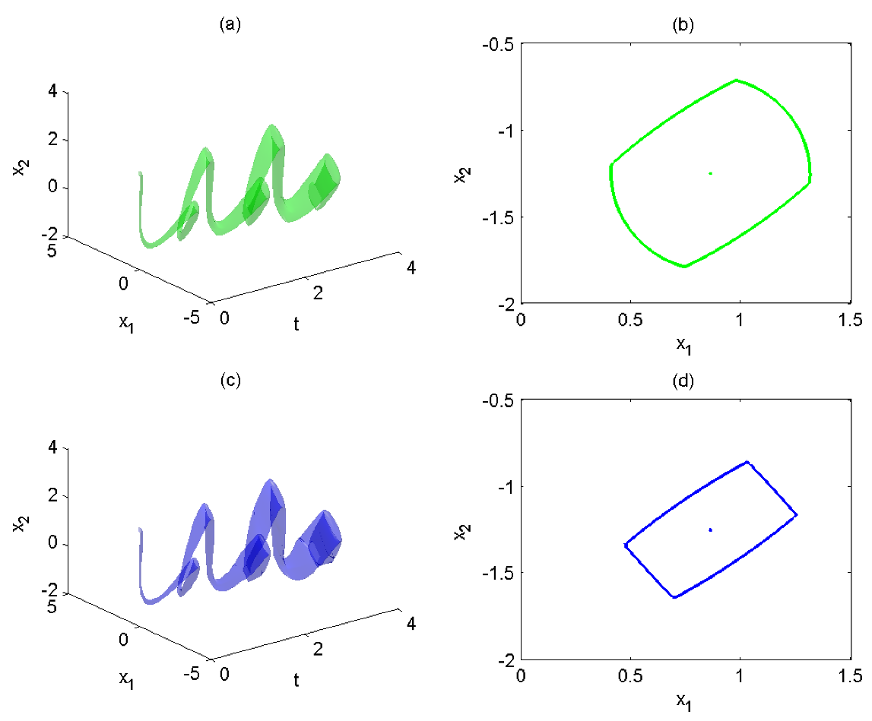
\includegraphics[height=10 cm]{reachmech.eps}}
\caption{Spring-mass system without disturbance:
(a) reach tube for time $t\in[0,4]$; (b) reach set at time $t=4$.
Spring-mass system with disturbance:
(c) reach tube for time $t\in[0,4]$; (d) reach set at time $t=4$.}
\label{mechreachfig}
\end{figure}

So far we considered an ideal system without any disturbance, such as friction.
We introduce disturbance to (\ref{spmass1}-\ref{spmass2}) by adding extra
terms, $v_1$ and $v_2$,
\begin{eqnarray}
m_1\ddot{x}_1+(k_1+k_2)x_1-k_2x_2 & = & u_1 + v_1, \label{smdist1}\\
m_2\ddot{x}_2-k_2x_1+(k_1+k_2)x_2 & = & u_2 + v_2, \label{smdist2}
\end{eqnarray}
which results in equation (\ref{spmassls}) getting an extra term
\[ \left[\begin{array}{cc}
0 & 0\\
0 & 0\\
1 & 0\\
0 & 1\end{array}\right]\left[\begin{array}{c}
v_1\\
v_2\end{array}\right]. \]
Assuming that $[v_1 ~~ v_2]^T$ is unknown but bounded by ellipsoid
$\EE(0, \frac{1}{4}I)$, we can compute the closed-loop reach set of the system
with disturbance.
\verbmcodef[Computation of the closed-loop reach set]
{mcodesnippets/s_chapter06_section02_snippet02.m}

Figure \ref{mechreachfig}(c) shows the reach set of the system
(\ref{smdist1}-\ref{smdist2}) evolving in time from $t=0$ to $t=4$.
Figure \ref{mechreachfig}(d) presents a snapshot of this reach set at time
$t=4$.



\section{Switched System}
By {\it switched systems} we mean systems whose dynamics
changes at known times. Consider the RLC circuit shown in figure \ref{rlcfig}.
It has two inputs - the voltage ($v$) and current ($i$) sources.
Define
\begin{itemize}
\item $x_1$ - voltage across capacitor $C_1$, so $C_1\dot{x}_1$ is
the corresponding current;
\item $x_2$ - voltage across capacitor $C_2$, so the corresponding
current is $C_2\dot{x}_2$.
\item $x_3$ - current through the inductor $L$, so the voltage across
the inductor is $L\dot{x}_3$.
\end{itemize}
\begin{figure}[htbp]
\centerline{
\includegraphics[height=5 cm]{rlc.eps}}
\caption{RLC circuit with two inputs.}
\label{rlcfig}
\end{figure}
Applying Kirchoff current and voltage laws we arrive at the linear system,
\begin{equation}
\left[\begin{array}{c}
\dot{x}_1\\
\dot{x}_2\\
\dot{x}_3\end{array}\right] = \left[\begin{array}{ccc}
-\frac{1}{R_1C_1} & 0 & -\frac{1}{C_1}\\
0 & 0 & \frac{1}{C_2}\\
\frac{1}{L} & -\frac{1}{L} & -\frac{R_2}{L}\end{array}\right]
\left[\begin{array}{c}
x_1\\
x_2\\
x_3\end{array}\right] + \left[\begin{array}{cc}
\frac{1}{R_1C_1} & \frac{1}{C_1}\\
0 & 0\\
0 & 0\end{array}\right]\left[\begin{array}{c}
v\\
i\end{array}\right]. \label{rlceq}
\end{equation}
The parameters $R_1$, $R_2$, $C_1$, $C_2$ and $L$, as well as the inputs,
may depend on time. Suppose, for time $0\leq t<2$, $R_1=2$ Ohm, $R_2=1$ Ohm,
$C_1=3$ F, $C_2=7$ F, $L=2$ H, both inputs, $v$ and $i$ are present and
bounded by ellipsoid $\EE(0,I)$; and for time $t\geq 2$,
$R_1=R_2=2$ Ohm, $C_1=C_2=3$ F, $L=6$ H, the current source is turned off,
and $|v|\leq 1$. Then, system (\ref{rlceq}) can be rewritten as
\begin{equation}
\left[\begin{array}{c}
\dot{x}_1\\
\dot{x}_2\\
\dot{x}_3\end{array}\right] = \left\{\begin{array}{ll}
\left[\begin{array}{ccc}
-\frac{1}{6} & 0 & -\frac{1}{3}\\
0 & 0 & \frac{1}{7}\\
\frac{1}{2} & -\frac{1}{2} & -\frac{1}{2}\end{array}\right]
\left[\begin{array}{c}
x_1\\
x_2\\
x_3\end{array}\right] + \left[\begin{array}{cc}
\frac{1}{6} & \frac{1}{3}\\
0 & 0\\
0 & 0\end{array}\right]\left[\begin{array}{c}
v\\
i\end{array}\right], & 0\leq t< 2, \\
\left[\begin{array}{ccc}
-\frac{1}{6} & 0 & -\frac{1}{3}\\
0 & 0 & \frac{1}{3}\\
\frac{1}{6} & -\frac{1}{6} & -\frac{1}{3}\end{array}\right]
\left[\begin{array}{c}
x_1\\
x_2\\
x_3\end{array}\right] + \left[\begin{array}{c}
\frac{1}{6} \\
0 \\
0 \end{array}\right]v, & 2\leq t. \end{array}\right.
\label{rlceq2}
\end{equation}
We can compute the reach set of (\ref{rlceq2}) for some time $t>2$, say, $t=3$.

\verbmcodef[Computation of the reach set for time interval]
{mcodesnippets/s_chapter06_section03_snippet01.m}

Figure \ref{rlcreachfig}(a) shows how the reach set projection
onto $(x_1, x_2)$ of system (\ref{rlceq2})
evolves in time from $t=0$  to $t=3$. The external reach set approximation
for the first dynamics is in red, the internal approximation is in green.
The dynamics switches at $t=2$.
The external reach set approximation for the second dynamics is in yellow,
its internal approximation is in blue.
The full three-dimensional external (yellow) and internal (blue)
approximations of the reach set are shown in figure \ref{rlcreachfig}(b).
\begin{figure}[htbp]
\centerline{
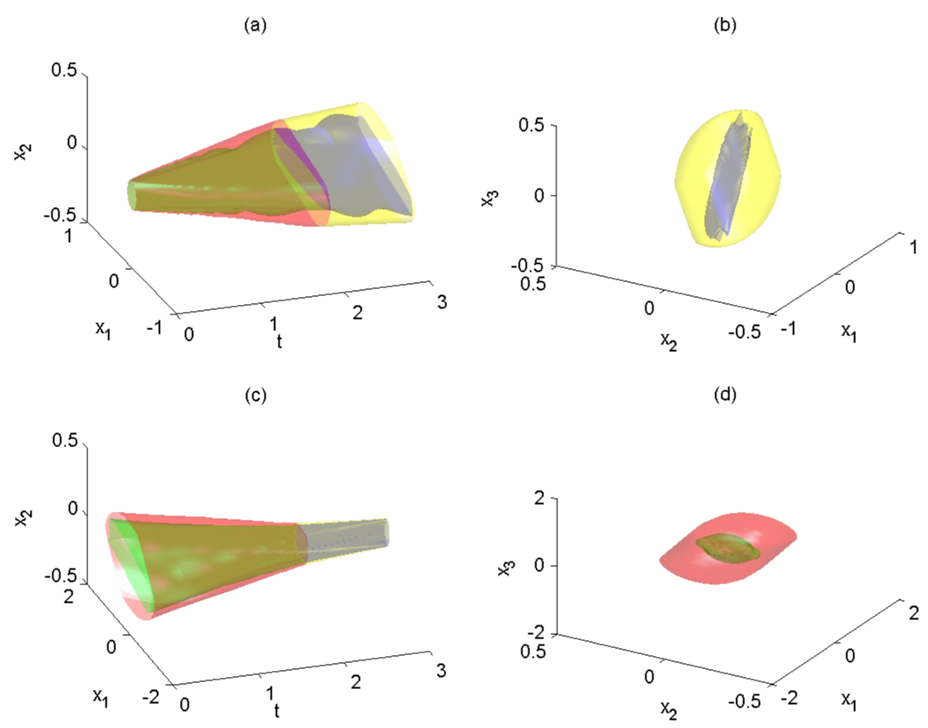
\includegraphics[height=10 cm]{rlcreach.eps}}
\caption{Forward and backward reach sets of the switched system
(external and internal approximations).
The dynamics switches at $t=2$.
\newline
(a) Forward reach set for the time interval $0\leq t\leq3$ projected onto
$(x_1,x_2)$ subspace.
\newline
(b) Forward reach set at $t=3$ in ${\bf R}^3$.
\newline
(c) Backward reach set evolving from $t=3$ to $t=0$ projected onto
$(x_1,x_2)$ subspace.
\newline
(d) Backward reach set at $t=0$ in ${\bf R}^3$.}
\label{rlcreachfig}
\end{figure}

To find out where the system should start at time $t=0$ in order to reach
a neighborhood {\tt M} of the origin at time $t=3$,
we compute the backward reach set from $t=3$ to $t=0$.
\verbmcodef[Computation of the backward reach set]
{mcodesnippets/s_chapter06_section03_snippet02.m}

Figure \ref{rlcreachfig}(c) presents the evolution of the reach set
projection onto $(x_1, x_2)$ in backward time.
Again, external and internal approximations corresponding
to the first dynamics are shown in red and green, and
to the second dynamics in yellow and blue. The
full dimensional backward reach set external and internal
approximations of system (\ref{rlceq2})
at time $t=0$ is shown in figure \ref{rlcreachfig}(d).



\section{Hybrid System}
There is no explicit implementation of the reachability analysis for hybrid
systems in the {\it Ellipsoidal Toolbox}.
Nonetheless, the operations of intersection available in the toolbox allow us
to work with certain class of hybrid systems, namely,
hybrid systems with affine continuous dynamics whose guards are
ellipsoids, hyperplanes, halfspaces or polytopes.

We  consider the {\it switching-mode model} of highway traffic
presented in \cite{xiaotian}. The highway segment is divided into $N$ cells
as shown in figure \ref{hwfig}. In this particular case, $N=4$.
The traffic density in cell $i$ is  $x_i$ vehicles per mile, $i=1,2,3,4$.
\begin{figure}[htbp]
\centerline{
\includegraphics[height=5 cm]{hw.eps}}
\caption{Highway model. Adapted from \cite{xiaotian}.}
\label{hwfig}
\end{figure}

Define
\begin{itemize}
\item $v_i$ - average  speed in mph,
in the $i$-th cell, $i=1,2,3,4$;
\item $w_i$ - backward congestion wave propagation speed in mph,
in the $i$-th highway cell, $i=1,2,3,4$;
\item $x_{Mi}$ - maximum allowed density in the $i$-th cell;
when this velue is reached, there is a traffic jam, $i=1,2,3,4$;
\item $d_i$ - length of $i$-th cell in miles, $i=1,2,3,4$;
\item $T_s$ - sampling time in hours;
\item $b$ - split ratio for the off-ramp;
\item $u_1$ - traffic flow coming into the highway segment,
in vehicles per hour (vph);
\item $u_2$ - traffic flow coming out of the highway segment (vph);
\item $u_3$ - on-ramp traffic flow (vph).
\end{itemize}
Highway traffic operates in two modes: {\it free-flow} in normal operation;
and {\it congested} mode, when there is a jam.
Traffic flow in free-flow mode is described by
\begin{eqnarray}
\left[\begin{array}{c}
x_1[t+1]\\
x_2[t+1]\\
x_3[t+1]\\
x_4[t+1]\end{array}\right] & = & \left[\begin{array}{cccc}
1-\frac{v_1T_s}{d_1} & 0 & 0 & 0\\
\frac{v_1T_s}{d_2} & 1-\frac{v_2T_s}{d_2} & 0 & 0\\
0 & \frac{v_2T_s}{d_3} & 1-\frac{v_3T_s}{d_3} & 0\\
0 & 0 & (1-b)\frac{v_3T_s}{d_4} & 1-\frac{v_4T_s}{d_4}\end{array}\right]
\left[\begin{array}{c}
x_1[t]\\
x_2[t]\\
x_3[t]\\
x_4[t]\end{array}\right] \nonumber\\
& + & \left[\begin{array}{ccc}
\frac{v_1T_s}{d_1} & 0 & 0\\
0 & 0 & \frac{v_2T_s}{d_2}\\
0 & 0 & 0\\
0 & 0 & 0\end{array}\right]\left[\begin{array}{c}
u_1\\
u_2\\
u_3\end{array}\right]. \label{fflow}
\end{eqnarray}
The equation for the congested mode is
\begin{eqnarray}
\left[\begin{array}{c}
x_1[t+1]\\
x_2[t+1]\\
x_3[t+1]\\
x_4[t+1]\end{array}\right] & = & \left[\begin{array}{cccc}
1-\frac{w_1T_s}{d_1} & \frac{w_2T_s}{d_1} & 0 & 0\\
0 & 1-\frac{w_2T_s}{d_2} & \frac{w_3T_s}{d_2} & 0\\
0 & 0 & 1-\frac{w_3T_s}{d_3} & \frac{1}{1-b}\frac{w_4T_s}{d_3}\\
0 & 0 & 0 & 1-\frac{w_4T_s}{d_4}\end{array}\right]
\left[\begin{array}{c}
x_1[t]\\
x_2[t]\\
x_3[t]\\
x_4[t]\end{array}\right] \nonumber\\
& + & \left[\begin{array}{ccc}
0 & 0 & \frac{w_1T_s}{d_1}\\
0 & 0 & 0\\
0 & 0 & 0\\
0 & -\frac{w_4T_s}{d_4} & 0\end{array}\right]\left[\begin{array}{c}
u_1\\
u_2\\
u_3\end{array}\right] \nonumber\\
& + & \left[\begin{array}{cccc}
\frac{w_1T_s}{d_1} & -\frac{w_2T_s}{d_1} & 0 & 0\\
0 & \frac{w_2T_s}{d_2} & -\frac{w_3T_s}{d_2} & 0\\
0 & 0 & \frac{w_3T_s}{d_3} & -\frac{1}{1-b}\frac{w_4T_s}{d_3}\\
0 & 0 & 0 & \frac{w_4T_s}{d_4}\end{array}\right]
\left[\begin{array}{c}
x_{M1}\\
x_{M2}\\
x_{M3}\\
x_{M4}\end{array}\right]. \label{cflow}
\end{eqnarray}
The switch from the free-flow to the congested mode occurs when the density
 $x_2$ reaches $x_{M2}$. In other words, the hyperplane
$H([0 ~ 1 ~ 0 ~ 0]^T, x_{M2})$ is the guard.

We indicate how to implement the reach set computation of this hybrid system.
We first define the two linear systems and the guard.
\verbmcodef[Reach set computation of the hybrid system]
{mcodesnippets/s_chapter06_section04_snippet01.m}

We assume that initially the system is in free-flow mode.
Given a set of initial conditions, we  compute the reach set according
to dynamics (\ref{fflow}) for certain number of time steps.
We will consider the external approximation of the reach set by a single
ellipsoid.
\verbmcodef[Get the external approximation of the reach set by a single
ellipsoid]{mcodesnippets/s_chapter06_section04_snippet02.m}

Having obtained the ellipsoidal array {\tt externalEllMat} representing the reach set
evolving in time, we  determine the  ellipsoids in the array that
intersect the guard.
\verbmcodef[Determination of  the  ellipsoids as an array that intersect the guard]{mcodesnippets/s_chapter06_section04_snippet03.m}

Analyzing the values in array {\tt dVec}, we conclude that the free-flow reach set
has nonempty intersection with hyperplane {\tt grdHyp} at $t=18$
for the first time, and at $t=68$ for the last time.
Between $t=18$ and
$t=68$ it crosses the guard. Figure \ref{hwreachfig}(a) shows the
free-flow reach set projection onto $(x_1,x_2,x_3)$ subspace for $t=10$,
before the guard crossing; figure \ref{hwreachfig}(b) for $t=50$,
during the guard crossing; and figure \ref{hwreachfig}(c) for $t=80$,
after the guard was crossed.
\begin{figure}[htbp]
\centerline{
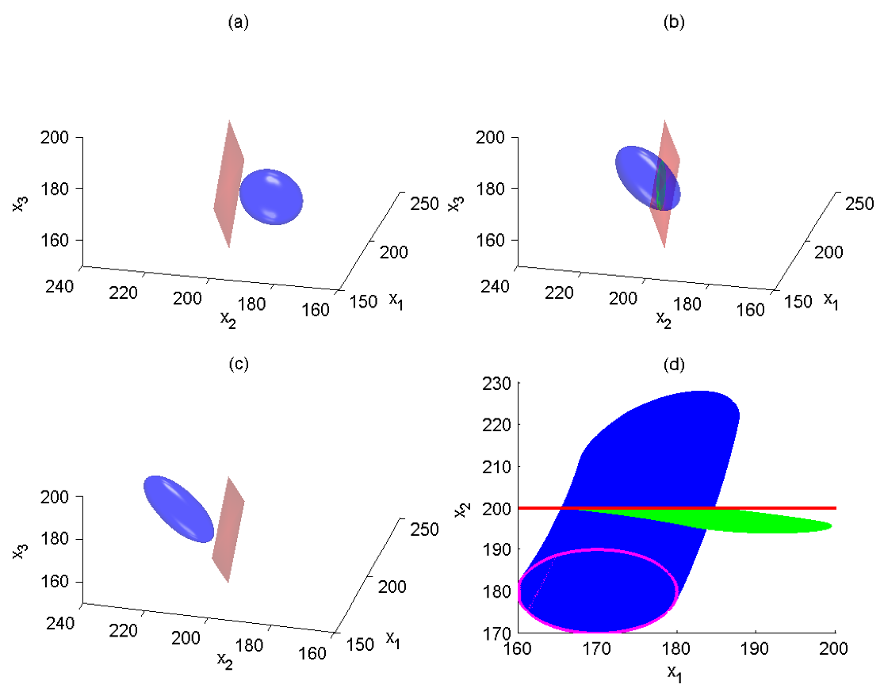
\includegraphics[height=10 cm]{hwreach.eps}}
\caption{Reach set of the free-flow system is blue, reach set of the congested
system is green, the guard is red.
\newline
(a) Reach set of the free-flow system at $t = 10$, before reaching the guard
(projection onto $(x_1,x_2,x_3)$).
\newline
(b) Reach set of the free-flow system at $t = 50$, crossing the guard.
(projection onto $(x_1,x_2,x_3)$).
\newline
(c) Reach set of the free-flow system at $t = 80$, after the guard is crossed.
(projection onto $(x_1,x_2,x_3)$).
\newline
(d) Reach set trace from $t=0$ to $t=100$, free-flow system in blue,
congested system in green; bounds of initial conditions are marked with magenta
(projection onto $(x_1,x_2)$).  }
\label{hwreachfig}
\end{figure}

For each time step that the intersection of the free-flow reach set and the
guard is nonempty, we establish a new initial time and a set of initial
conditions for the reach set computation according to dynamics (\ref{cflow}).
The initial time is the array index minus one, and the set of initial
conditions is the intersection of the free-flow reach set with the guard.
\verbmcodef[The union of reach sets in array]{mcodesnippets/s_chapter06_section04_snippet04.m}

The union of reach sets in array {\tt crs} forms the reach set for
the congested dynamics.

A summary of
 the reach set computation of the
linear hybrid system (\ref{fflow}-\ref{cflow}) for $N=100$ time steps
with one guard crossing is given in figure \ref{hwreachfig}(d),
which shows the projection of the reach set trace onto $(x_1,x_2)$ subspace.
The system starts evolving in time in free-flow mode from a set of
initial conditions at $t=0$, whose boundary is shown in magenta.
The free-flow reach set evolving from $t=0$ to $t=100$ is shown in blue.
Between  $t=18$ and $t=68$ the free-flow reach set crosses the guard.
The guard is shown in red.
For each  nonempty intersection of the free-flow reach set and the guard,
the congested mode reach set starts evolving in time until $t=100$.
All the congested mode reach sets are shown in green.
Observe that in the congested mode, the density $x_2$ in the congested part
 decreases slightly, while the density $x_1$ upstream of the congested part
 increases.
The blue  set above the guard is not actually reached,
because the state evolves according to the green region.


\chapter{Summary and Outlook}\label{ch_summary}
Although some of the operations with ellipsoids are present in the
commercial Geometric Bounding Toolbox \cite{VERES_KUNSEVICH_VALYI_HERMSMEYER_WALL_GEOMETRIC_BOUNDING_TOOLBOX, GEOMETRIC_BOUNDING_TOOLBOX_HOMEPAGE}, the
ellipsoid-related functionality of that toolbox is rather limited.

{\it Ellipsoidal Toolbox} is the first free MATLAB package that
implements ellipsoidal calculus and uses ellipsoidal methods
for reachability analysis of continuous- and discrete-time affine
systems, continuous-time linear systems with disturbances and switched
systems, whose dynamics changes at known times.
The reach set computation for hybrid systems whose guards are hyperplanes
or polyhedra is not implemented explicitly, but the tool for such computation
exists, namely, the operations of intersection of ellipsoid with hyperplane
and ellipsoid with halfspace.




\chapter*{Acknowledgement}
\addcontentsline{toc}{chapter}{Acknowledgement}
The authors would like to thank Alexander B. Kurzhanski,
Manfred Morari, Johan L{\"o}fberg, Michal Kvasnica and Goran Frehse
for their support of this work by useful advice and encouragement.


\addcontentsline{toc}{chapter}{Bibliography}
\bibliography{et}
\todo[inline]{Added bib file}
\appendix
\chapter{Function Reference}\label{appendix_a}
\section{ellipsoid}\label{secClassDescr:ellipsoid}
\subsection{\texorpdfstring{ellipsoid.calcGrid}{calcGrid}}\label{method:ellipsoid.calcGrid}
\begin{verbatim}
CALCGRID - computes grid of 2d or 3d sphere and vertices for each face
           in the grid with number of points taken from ellObj
           nPlot2dPoints or nPlot3dPoints parameters
\end{verbatim}
\subsection{\texorpdfstring{ellipsoid.checkIsMe}{checkIsMe}}\label{method:ellipsoid.checkIsMe}
\begin{verbatim}
CHECKISME - determine whether input object is ellipsoid. And display
            message and abort function if input object
            is not ellipsoid

Input:
  regular:
      someObjArr: any[] - any type array of objects.

Example:
  ellObj = ellipsoid([1; 2], eye(2));
  ellipsoid.checkIsMe(ellObj)
\end{verbatim}
\subsection{\texorpdfstring{ellipsoid.contents}{contents}}\label{method:ellipsoid.contents}
\begin{verbatim}
Ellipsoid library of the Ellipsoidal Toolbox.


Constructor and data accessing functions:
-----------------------------------------
 ellipsoid    - Constructor of ellipsoid object.
 double       - Returns parameters of ellipsoid, i.e. center and shape
                matrix.
 parameters   - Same function as 'double'(legacy matter).
 dimension    - Returns dimension of ellipsoid and its rank.
 isdegenerate - Checks if ellipsoid is degenerate.
 isempty      - Checks if ellipsoid is empty.
 maxeig       - Returns the biggest eigenvalue of the ellipsoid.
 mineig       - Returns the smallest eigenvalue of the ellipsoid.
 trace        - Returns the trace of the ellipsoid.
 volume       - Returns the volume of the ellipsoid.


Overloaded operators and functions:
-----------------------------------
 eq      - Checks if two ellipsoids are equal.
 ne      - The opposite of 'eq'.
 gt, ge  - E1 > E2 (E1 >= E2) checks if, given the same center ellipsoid
           E1 contains E2.
 lt, le  - E1 < E2 (E1 <= E2) checks if, given the same center ellipsoid
           E2 contains E1.
 mtimes  - Given matrix A in R^(mxn) and ellipsoid E in R^n, returns
           (A * E).
 plus    - Given vector b in R^n and ellipsoid E in R^n, returns (E + b).
 minus   - Given vector b in R^n and ellipsoid E in R^n, returns (E - b).
 uminus  - Changes the sign of the center of ellipsoid.
 display - Displays the details about given ellipsoid object.
 inv     - inverts the shape matrix of the ellipsoid.
 plot    - Plots ellipsoid in 1D, 2D and 3D.


Geometry functions:
-------------------
 move2origin        - Moves the center of ellipsoid to the origin.
 shape              - Same as 'mtimes', but modifies only shape matrix of
                      the ellipsoid leaving its center as is.
 rho                - Computes the value of support function and
                      corresponding boundary point of the ellipsoid in
                      the given direction.
 polar              - Computes the polar ellipsoid to an ellipsoid that
                      contains the origin.
 projection         - Projects the ellipsoid onto a subspace specified
                      by  orthogonal basis vectors.
 minksum            - Computes and plots the geometric (Minkowski) sum of
                      given ellipsoids in 1D, 2D and 3D.
 minksum_ea         - Computes the external ellipsoidal approximation of
                      geometric sum of given ellipsoids in given
                      direction.
 minksum_ia         - Computes the internal ellipsoidal approximation of
                      geometric sum of given ellipsoids in given
                      direction.
 minkdiff           - Computes and plots the geometric (Minkowski)
                      difference of given ellipsoids in 1D, 2D and 3D.
 minkdiff_ea        - Computes the external ellipsoidal approximation of
                      geometric difference of two ellipsoids in given
                      direction.
 minkdiff_ia        - Computes the internal ellipsoidal approximation of
                      geometric difference of two ellipsoids in given
                      direction
 minkpm             - Computes and plots the geometric (Minkowski)
                      difference of a geometric sum of ellipsoids and a
                      single ellipsoid in 1D, 2D and 3D.
 minkpm_ea          - Computes the external ellipsoidal approximation of
                      the geometric difference of a geometric sum of
                      ellipsoids and a single ellipsoid in given
                      direction.
 minkpm_ia          - Computes the internal ellipsoidal approximation of
                      the geometric difference of a geometric sum of
                      ellipsoids and a single ellipsoid in given
                      direction.
 minkmp             - Computes and plots the geometric (Minkowski) sum of
                      a geometric difference of two single ellipsoids and
                      a geometric sum of ellipsoids in 1D, 2D and 3D.
 minkmp_ea          - Computes the external ellipsoidal approximation of
                      the geometric sum of a geometric difference of two
                      single ellipsoids and a geometric sum of ellipsoids
                      in given direction.
 minkmp_ia          -  Computes the internal ellipsoidal approximation of
                      the geometric sum of a geometric difference of
                      two single ellipsoids and a geometric sum of ellipsoids
                      in given direction.
 isbaddirection     - Checks if ellipsoidal approximation of geometric difference
                      of two ellipsoids in the given direction can be computed.
 doesIntersectionContain           - Checks if the union or intersection of
                      ellipsoids or polytopes lies inside the intersection
                      of given ellipsoids.
 isinternal         - Checks if given vector belongs to the union or intersection
                      of given ellipsoids.
 distance           - Computes the distance from ellipsoid to given point,
                      ellipsoid, hyperplane or polytope.
 intersect          - Checks if the union or intersection of ellipsoids intersects
                      with given ellipsoid, hyperplane, or polytope.
 intersection_ea    - Computes the minimal volume ellipsoid containing intersection
                      of two ellipsoids, ellipsoid and halfspace, or ellipsoid
                      and polytope.
 intersection_ia    - Computes the maximal ellipsoid contained inside the
                      intersection of two ellipsoids, ellipsoid and halfspace
                      or ellipsoid and polytope.
 ellintersection_ia - Computes maximum volume ellipsoid that is contained
                      in the intersection of given ellipsoids (can be more than 2).
 ellunion_ea        - Computes minimum volume ellipsoid that contains
                      the union of given ellipsoids.
 hpintersection     - Computes the intersection of ellipsoid with hyperplane.
\end{verbatim}
\subsection{\texorpdfstring{ellipsoid.dimension}{dimension}}\label{method:ellipsoid.dimension}
\begin{verbatim}
DIMENSION - returns the dimension of the space in which the ellipsoid is
            defined and the actual dimension of the ellipsoid.

Input:
  regular:
    myEllArr: ellipsoid[nDims1,nDims2,...,nDimsN] - array of ellipsoids.

Output:
  regular:
    dimArr: double[nDims1,nDims2,...,nDimsN] - space dimensions.

  optional:
    rankArr: double[nDims1,nDims2,...,nDimsN] - dimensions of the
           ellipsoids in myEllArr.

Example:
  firstEllObj = ellipsoid();
  tempMatObj = [3 1; 0 1; -2 1];
  secEllObj = ellipsoid([1; -1; 1], tempMatObj*tempMatObj');
  thirdEllObj = ellipsoid(eye(2));
  fourthEllObj = ellipsoid(0);
  ellMat = [firstEllObj secEllObj; thirdEllObj fourthEllObj];
  [dimMat, rankMat] = ellMat.dimension()

  dimMat =

     0     3
     2     1

  rankMat =

     0     2
     2     0
\end{verbatim}
\subsection{\texorpdfstring{ellipsoid.disp}{disp}}\label{method:ellipsoid.disp}
\begin{verbatim}
DISP - Displays ellipsoid object.

Input:
  regular:
    myEllMat: ellipsoid [mRows, nCols] - matrix of ellipsoids.

Example:
  ellObj = ellipsoid([-2; -1], [2 -1; -1 1]);
  disp(ellObj)

  Ellipsoid with parameters
  Center:
      -2
      -1

  Shape Matrix:
       2    -1
      -1     1
\end{verbatim}
\subsection{\texorpdfstring{ellipsoid.display}{display}}\label{method:ellipsoid.display}
\begin{verbatim}
DISPLAY - Displays the details of the ellipsoid object.

Input:
  regular:
      myEllMat: ellipsoid [mRows, nCols] - matrix of ellipsoids.

Example:
  ellObj = ellipsoid([-2; -1], [2 -1; -1 1]);
  display(ellObj)

  ellObj =

  Center:
      -2
      -1

  Shape Matrix:
       2    -1
      -1     1

  Nondegenerate ellipsoid in R^2.
\end{verbatim}
\subsection{\texorpdfstring{ellipsoid.distance}{distance}}\label{method:ellipsoid.distance}
\begin{verbatim}
DISTANCE - computes distance between the given ellipsoid (or array of
           ellipsoids) to the specified object (or arrays of objects):
           vector, ellipsoid, hyperplane or polytope.

Input:
  regular:
      ellObjArr: ellipsoid [nDims1, nDims2,..., nDimsN] -  array of
         ellipsoids of the same dimension.
      objArray: double / ellipsoid / hyperplane / polytope [nDims1,
          nDims2,..., nDimsN] - array of vectors or ellipsoids or
          hyperplanes or polytopes. If number of elements in objArray
          is more than 1, then it must be equal to the number of elements
          in ellObjArr.

  optional:
      isFlagOn: logical[1,1] - if true then distance is  computed in
          ellipsoidal metric, if false - in Euclidean metric (by default
          isFlagOn=false).

Output:
  regular:
    distValArray: double [nDims1, nDims2,..., nDimsN] - array of pairwise
          calculated distances.
          Negative distance value means
              for ellipsoid and vector: vector belongs to the ellipsoid,
              for ellipsoid and hyperplane: ellipsoid intersects the
                  hyperplane.
              Zero distance value means for ellipsoid and vector: vector
                  is aboundary point of the ellipsoid,
              for ellipsoid and hyperplane: ellipsoid  touches the
                  hyperplane.
  optional:
      statusArray: double [nDims1, nDims2,..., nDimsN] - array of time of
          computation of ellipsoids-vectors or ellipsoids-ellipsoids
          distances, or status of cvx solver for ellipsoids-polytopes
          distances.

Literature:
 1. Lin, A. and Han, S. On the Distance between Two Ellipsoids.
    SIAM Journal on Optimization, 2002, Vol. 13, No. 1 : pp. 298-308
 2. Stanley Chan, "Numerical method for Finding Minimum Distance to an
    Ellipsoid".
    http://videoprocessing.ucsd.edu/~stanleychan/publication/...
    unpublished/Ellipse.pdf

Example:
  ellObj = ellipsoid([-2; -1], [4 -1; -1 1]);
  tempMat = [1 1; 1 -1; -1 1; -1 -1]';
  distVec = ellObj.distance(tempMat)

  distVec =

       2.3428    1.0855    1.3799    -1.0000
\end{verbatim}
\subsection{\texorpdfstring{ellipsoid.doesContain}{doesContain}}\label{method:ellipsoid.doesContain}
\begin{verbatim}
DOESCONTAIN - checks if one ellipsoid contains the other ellipsoid or
              polytope. The condition for E1 = firstEllArr to contain
              E2 = secondEllArr is
              min(rho(l | E1) - rho(l | E2)) > 0, subject to <l, l> = 1.
              How checked if ellipsoid contains polytope is explained in
              doesContainPoly.
Input:
  regular:
      firstEllArr: ellipsoid [nDims1,nDims2,...,nDimsN]/[1,1] - first
          array of ellipsoids.
      secondObjArr: ellipsoid [nDims1,nDims2,...,nDimsN]/
          polytope[nDims1,nDims2,...,nDimsN]/[1,1] - array of the same
          size as firstEllArr or single ellipsoid or polytope.

   properties:
      mode: char[1, 1] - 'u' or 'i', go to description.
      computeMode: char[1,] - 'highDimFast' or 'lowDimFast'. Determines,
          which way function is computed, when secObjArr is polytope. If
          secObjArr is ellipsoid computeMode is ignored. 'highDimFast'
          works  faster for  high dimensions, 'lowDimFast' for low. If
          this property is omitted if dimension of ellipsoids is greater
          then 10, then 'hightDimFast' is choosen, otherwise -
          'lowDimFast'

Output:
  isPosArr: logical[nDims1,nDims2,...,nDimsN],
      resArr(iCount) = true - firstEllArr(iCount)
      contains secondObjArr(iCount), false - otherwise.

Example:
  firstEllObj = ellipsoid([-2; -1], [2 -1; -1 1]);
  secEllObj = ellipsoid([-1;0], eye(2));
  doesContain(firstEllObj,secEllObj)

  ans =

       0
\end{verbatim}
\subsection{\texorpdfstring{ellipsoid.doesIntersectionContain}{doesIntersectionContain}}\label{method:ellipsoid.doesIntersectionContain}
\begin{verbatim}
DOESINTERSECTIONCONTAIN - checks if the intersection of ellipsoids
                          contains the union or intersection of given
                          ellipsoids or polytopes.

  res = DOESINTERSECTIONCONTAIN(fstEllArr, secEllArr, mode)
      Checks if the union
      (mode = 'u') or intersection (mode = 'i') of ellipsoids in
      secEllArr lies inside the intersection of ellipsoids in
      fstEllArr. Ellipsoids in fstEllArr and secEllArr must be
      of the same dimension. mode = 'u' (default) - union of
      ellipsoids in secEllArr. mode = 'i' - intersection.
  res = DOESINTERSECTIONCONTAIN(fstEllArr, secPolyArr, mode)
       Checks if the union
      (mode = 'u') or intersection (mode = 'i')  of polytopes in
      secPolyArr lies inside the intersection of ellipsoids in
      fstEllArr. Ellipsoids in fstEllArr and polytopes in secPolyArr
      must be of the same dimension. mode = 'u' (default) - union of
      polytopes in secPolyMat. mode = 'i' - intersection.

  To check if the union of ellipsoids secEllArr belongs to the
  intersection of ellipsoids fstEllArr, it is enough to check that
  every ellipsoid of secEllMat is contained in every
  ellipsoid of fstEllArr.
  Checking if the intersection of ellipsoids in secEllMat is inside
  intersection fstEllMat can be formulated as quadratically
  constrained quadratic programming (QCQP) problem.

  Let fstEllArr(iEll) = E(q, Q) be an ellipsoid with center q and shape
  matrix Q. To check if this ellipsoid contains the intersection of
  ellipsoids in secObjArr:
  E(q1, Q1), E(q2, Q2), ..., E(qn, Qn), we define the QCQP problem:
                    J(x) = <(x - q), Q^(-1)(x - q)> --> max
  with constraints:
                    <(x - q1), Q1^(-1)(x - q1)> <= 1   (1)
                    <(x - q2), Q2^(-1)(x - q2)> <= 1   (2)
                    ................................
                    <(x - qn), Qn^(-1)(x - qn)> <= 1   (n)

  If this problem is feasible, i.e. inequalities (1)-(n) do not
  contradict, or, in other words, intersection of ellipsoids
  E(q1, Q1), E(q2, Q2), ..., E(qn, Qn) is nonempty, then we can find
  vector y such that it satisfies inequalities (1)-(n)
  and maximizes function J. If J(y) <= 1, then ellipsoid E(q, Q)
  contains the given intersection, otherwise, it does not.

  The intersection of polytopes is a polytope, which is computed
  by the standard routine of MPT. How checked if intersection of
  ellipsoids contains polytope is explained in doesContainPoly.

  Checking if the union of polytopes belongs to the intersection
  of ellipsoids is the same as checking if its convex hull belongs
  to this intersection.

Input:
  regular:
      fstEllArr: ellipsoid [nDims1,nDims2,...,nDimsN] - array of ellipsoids
          of the same size.
      secEllArr: ellipsoid /
          polytope [nDims1,nDims2,...,nDimsN] - array of ellipsoids or
          polytopes of the same sizes.

          note: if mode == 'i', then fstEllArr, secEllVec should be
              array.

  properties:
      mode: char[1, 1] - 'u' or 'i', go to description.
      computeMode: char[1,] - 'highDimFast' or 'lowDimFast'. Determines,
          which way function is computed, when secObjArr is polytope. If
          secObjArr is ellipsoid computeMode is ignored. 'highDimFast'
          works  faster for  high dimensions, 'lowDimFast' for low. If
          this property is omitted if dimension of ellipsoids is greater
          then 10, then 'hightDimFast' is choosen, otherwise -
          'lowDimFast'


Output:
  res: double[1, 1] - result:
      -1 - problem is infeasible, for example, if s = 'i',
          but the intersection of ellipsoids in E2 is an empty set;
      0 - intersection is empty;
      1 - if intersection is nonempty.
  status: double[0, 0]/double[1, 1] - status variable. status is empty
      if mode == 'u' or mSecRows == nSecCols == 1.

Example:
  firstEllObj = [0 ; 0] + ellipsoid(eye(2, 2));
  secEllObj = [0 ; 0] + ellipsoid(2*eye(2, 2));
  thirdEllObj = [1; 0] + ellipsoid(0.5 * eye(2, 2));
  secEllObj.doesIntersectionContain([firstEllObj secEllObj], 'i')

  ans =

       1
\end{verbatim}
\subsection{\texorpdfstring{ellipsoid.double}{double}}\label{method:ellipsoid.double}
\begin{verbatim}
DOUBLE - returns parameters of the ellipsoid.

Input:
  regular:
      myEll: ellipsoid [1, 1] - single ellipsoid of dimention nDims.


Output:
  myEllCentVec: double[nDims, 1] - center of the ellipsoid myEll.

  myEllShMat: double[nDims, nDims] - shape matrix of the ellipsoid myEll.

Example:
  ellObj = ellipsoid([-2; -1], [2 -1; -1 1]);
  [centVec, shapeMat] = double(ellObj)
  centVec =

      -2
      -1


  shapeMat =

       2    -1
      -1     1
\end{verbatim}
\subsection{\texorpdfstring{ellipsoid.ellbndr\_2d}{ellbndr\_2d}}\label{method:ellipsoid.ellbndr2d}
\begin{verbatim}
ELLBNDR_2D - compute the boundary of 2D ellipsoid. Private method.

Input:
  regular:
      myEll: ellipsoid [1, 1]- ellipsoid of the dimention 2.
  optional:
      nPoints: number of boundary points

Output:
  regular:
      bpMat: double[nPoints,2] - boundary points of ellipsoid
  optional:
      fVec: double[1,nFaces] - indices of points in each face of
          bpMat graph
\end{verbatim}
\subsection{\texorpdfstring{ellipsoid.ellbndr\_3d}{ellbndr\_3d}}\label{method:ellipsoid.ellbndr3d}
\begin{verbatim}
ELLBNDR_3D - compute the boundary of 3D ellipsoid.

Input:
  regular:
      myEll: ellipsoid [1, 1]- ellipsoid of the dimention 3.

  optional:
      nPoints: number of boundary points

Output:
  regular:
      bpMat: double[nPoints,3] - boundary points of ellipsoid
  optional:
      fMat: double[nFaces,3] - indices of face verties in bpMat
\end{verbatim}
\subsection{\texorpdfstring{ellipsoid.ellintersection\_ia}{ellintersection\_ia}}\label{method:ellipsoid.ellintersectionia}
\begin{verbatim}
ELLINTERSECTION_IA - computes maximum volume ellipsoid that is contained
                     in the intersection of given ellipsoids.


Input:
  regular:
      inpEllArr: ellipsoid [nDims1,nDims2,...,nDimsN] - array of
          ellipsoids of the same dimentions.

Output:
  outEll: ellipsoid [1, 1] - resulting maximum volume ellipsoid.

Example:
  firstEllObj = ellipsoid([-1; 1], [2 0; 0 3]);
  secEllObj = ellipsoid([1 2], eye(2);
  ellVec = [firstEllObj secEllObj];
  resEllObj = ellintersection_ia(ellVec)

  resEllObj =

  Center:
      0.1847
      1.6914

  Shape Matrix:
      0.0340   -0.0607
     -0.0607    0.1713

  Nondegenerate ellipsoid in R^2.
\end{verbatim}
\subsection{\texorpdfstring{ellipsoid.ellipsoid}{ellipsoid}}\label{method:ellipsoid.ellipsoid}
\begin{verbatim}
ELLIPSOID - constructor of the ellipsoid object.

  Ellipsoid E = { x in R^n : <(x - q), Q^(-1)(x - q)> <= 1 }, with current
      "Properties". Here q is a vector in R^n, and Q in R^(nxn) is positive
      semi-definite matrix

  ell = ELLIPSOID - Creates an empty ellipsoid

  ell = ELLIPSOID(shMat) - creates an ellipsoid with shape matrix shMat,
      centered at 0

   ell = ELLIPSOID(centVec, shMat) - creates an ellipsoid with shape matrix
      shMat and center centVec

  ell = ELLIPSOID(centVec, shMat, 'propName1', propVal1,...,
      'propNameN',propValN) - creates an ellipsoid with shape
      matrix shMat, center centVec and propName1 = propVal1,...,
      propNameN = propValN. In other cases "Properties"
      are taken from current values stored in
      elltool.conf.Properties.
  ellMat = Ellipsoid(centVecArray, shMatArray,
      ['propName1', propVal1,...,'propNameN',propValN]) -
      creates an array (possibly multidimensional) of
      ellipsoids with centers centVecArray(:,dim1,...,dimn)
      and matrices shMatArray(:,:,dim1,...dimn) with
      properties if given.

  These parameters can be accessed by DOUBLE(E) function call.
  Also, DIMENSION(E) function call returns the dimension of
  the space in which ellipsoid E is defined and the actual
  dimension of the ellipsoid; function ISEMPTY(E) checks if
  ellipsoid E is empty; function ISDEGENERATE(E) checks if
  ellipsoid E is degenerate.

Input:
  Case1:
    regular:
      shMatArray: double [nDim, nDim] /
          double [nDim, nDim, nDim1,...,nDimn] -
          shape matrices array

  Case2:
    regular:
      centVecArray: double [nDim,1] /
          double [nDim, 1, nDim1,...,nDimn] -
          centers array
      shMatArray: double [nDim, nDim] /
          double [nDim, nDim, nDim1,...,nDimn] -
          shape matrices array


  properties:
      absTol: double [1,1] - absolute tolerance with default value 10^(-7)
      relTol: double [1,1] - relative tolerance with default value 10^(-5)
      nPlot2dPoints: double [1,1] - number of points for 2D plot with
          default value 200
      nPlot3dPoints: double [1,1] - number of points for 3D plot with
           default value 200.

Output:
  ellMat: ellipsoid [1,1] / ellipsoid [nDim1,...nDimn] -
      ellipsoid with specified properties
      or multidimensional array of ellipsoids.

Example:
  ellObj = ellipsoid([1 0 -1 6]', 9*eye(4));
\end{verbatim}
\subsection{\texorpdfstring{ellipsoid.ellunion\_ea}{ellunion\_ea}}\label{method:ellipsoid.ellunionea}
\begin{verbatim}
ELLUNION_EA - computes minimum volume ellipsoid that contains union
              of given ellipsoids.

Input:
  regular:
      inpEllMat: ellipsoid [nDims1,nDims2,...,nDimsN] - array of
          ellipsoids of the same dimentions.

Output:
  outEll: ellipsoid [1, 1] - resulting minimum volume ellipsoid.

Example:
  firstEllObj = ellipsoid([-1; 1], [2 0; 0 3]);
  secEllObj = ellipsoid([1 2], eye(2));
  ellVec = [firstEllObj secEllObj];
  resEllObj = ellunion_ea(ellVec)
  resEllObj =

  Center:
     -0.3188
      1.2936

  Shape Matrix:
      5.4573    1.3386
      1.3386    4.1037

  Nondegenerate ellipsoid in R^2.
\end{verbatim}
\subsection{\texorpdfstring{ellipsoid.fromRepMat}{fromRepMat}}\label{method:ellipsoid.fromRepMat}
\begin{verbatim}
FROMREPMAT - returns array of equal ellipsoids the same
             size as stated in sizeVec argument

  ellArr = fromRepMat(sizeVec) - creates an array  size
           sizeVec of empty ellipsoids.

  ellArr = fromRepMat(shMat,sizeVec) - creates an array
           size sizeVec of ellipsoids with shape matrix
           shMat.

  ellArr = fromRepMat(cVec,shMat,sizeVec) - creates an
           array size sizeVec of ellipsoids with shape
           matrix shMat and center cVec.

Input:
  Case1:
      regular:
          sizeVec: double[1,n] - vector of size, have
          integer values.

  Case2:
      regular:
          shMat: double[nDim, nDim] - shape matrix of
          ellipsoids.
          sizeVec: double[1,n] - vector of size, have
          integer values.

  Case3:
      regular:
          cVec: double[nDim,1] - center vector of
          ellipsoids
          shMat: double[nDim, nDim] - shape matrix of
          ellipsoids.
          sizeVec: double[1,n] - vector of size, have
          integer values.

  properties:
      absTol: double [1,1] - absolute tolerance with default
          value 10^(-7)
      relTol: double [1,1] - relative tolerance with default
          value 10^(-5)
      nPlot2dPoints: double [1,1] - number of points for 2D plot
          with default value 200
      nPlot3dPoints: double [1,1] - number of points for 3D plot
          with default value 200.
\end{verbatim}
\subsection{\texorpdfstring{ellipsoid.fromStruct}{fromStruct}}\label{method:ellipsoid.fromStruct}
\begin{verbatim}
fromStruct -- converts structure array into ellipsoid array.

Input:
  regular:
      SEllArr: struct [nDim1, nDim2, ...] - array
          of structures with the following fields:

      q: double[1, nEllDim] - the center of ellipsoid
      Q: double[nEllDim, nEllDim] - the shape matrix of ellipsoid
Output:
      ellArr: ellipsoid [nDim1, nDim2, ...] - ellipsoid array with size of
          SEllArr.

Example:
s = struct('Q', eye(2), 'q', [0 0]);
ellipsoid.fromStruct(s)

-------ellipsoid object-------
Properties:
   |
   |-- actualClass : 'ellipsoid'
   |--------- size : [1, 1]

Fields (name, type, description):
    'Q'    'double'    'Configuration matrix'
    'q'    'double'    'Center'

Data:
   |
   |-- q : [0 0]
   |       -----
   |-- Q : |1|0|
   |       |0|1|
   |       -----
\end{verbatim}
\subsection{\texorpdfstring{ellipsoid.getAbsTol}{getAbsTol}}\label{method:ellipsoid.getAbsTol}
\begin{verbatim}
GETABSTOL - gives the array of absTol for all elements in ellArr

Input:
  regular:
      ellArr: ellipsoid[nDim1, nDim2, ...] - multidimension array
          of ellipsoids
  optional
      fAbsTolFun: function_handle[1,1] - function that apply
          to the absTolArr. The default is @min.

Output:
  regular:
      absTolArr: double [absTol1, absTol2, ...] - return absTol for
          each element in ellArr
  optional:
      absTol: double[1,1] - return result of work fAbsTolFun with
          the absTolArr

Usage:
  use [~,absTol] = ellArr.getAbsTol() if you want get only
      absTol,
  use [absTolArr,absTol] = ellArr.getAbsTol() if you want get
      absTolArr and absTol,
  use absTolArr = ellArr.getAbsTol() if you want get only absTolArr

Example:
  firstEllObj = ellipsoid([-1; 1], [2 0; 0 3]);
  secEllObj = ellipsoid([1 2], eye(2));
  ellVec = [firstEllObj secEllObj];
  absTolVec = ellVec.getAbsTol()

  absTolVec =

     1.0e-07 *

      1.0000    1.0000
\end{verbatim}
\subsection{\texorpdfstring{ellipsoid.getBoundary}{getBoundary}}\label{method:ellipsoid.getBoundary}
\begin{verbatim}
GETBOUNDARY - computes the boundary of an ellipsoid.

Input:
  regular:
      myEll: ellipsoid [1, 1]- ellipsoid of the dimention 2 or 3.
  optional:
      nPoints: number of boundary points

Output:
   bpMat: double[nPoints, nDims] - boundary points of ellipsoid.
   fMat: double[nFaces, nDims] - indices of points in each face of bpMat graph.
\end{verbatim}
\subsection{\texorpdfstring{ellipsoid.getBoundaryByFactor}{getBoundaryByFactor}}\label{method:ellipsoid.getBoundaryByFactor}
\begin{verbatim}
  GETBOUNDARYBYFACTOR - computes grid of 2d or 3d ellipsoid and vertices
                        for each face in the grid
\end{verbatim}
\subsection{\texorpdfstring{ellipsoid.getCenterVec}{getCenterVec}}\label{method:ellipsoid.getCenterVec}
\begin{verbatim}
GETCENTERVEC - returns centerVec vector of given ellipsoid

Input:
  regular:
     self: ellipsoid[1,1]

Output:
  centerVecVec: double[nDims,1] - centerVec of ellipsoid

Example:
  ellObj = ellipsoid([1; 2], eye(2));
  getCenterVec(ellObj)

  ans =

       1
       2
\end{verbatim}
\subsection{\texorpdfstring{ellipsoid.getCopy}{getCopy}}\label{method:ellipsoid.getCopy}
\begin{verbatim}
GETCOPY - gives array the same size as ellArr with copies of elements of
          ellArr.

Input:
  regular:
      ellArr: ellipsoid[nDim1, nDim2,...] - multidimensional array of
          ellipsoids.

Output:
  copyEllArr: ellipsoid[nDim1, nDim2,...] - multidimension array of
      copies of elements of ellArr.

Example:
  firstEllObj = ellipsoid([-1; 1], [2 0; 0 3]);
  secEllObj = ellipsoid([1; 2], eye(2));
  ellVec = [firstEllObj secEllObj];
  copyEllVec = getCopy(ellVec)

  copyEllVec =
  1x2 array of ellipsoids.
\end{verbatim}
\subsection{\texorpdfstring{ellipsoid.getInv}{getInv}}\label{method:ellipsoid.getInv}
\begin{verbatim}
GETINV - do the same as INV method: inverts shape matrices of ellipsoids
      in the given array, with only difference, that it doesn't modify
      input array of ellipsoids.

Input:
  regular:
    myEllArr: ellipsoid [nDims1,nDims2,...,nDimsN] - array of ellipsoids.

Output:
   invEllArr: ellipsoid [nDims1,nDims2,...,nDimsN] - array of ellipsoids
      with inverted shape matrices.

Example:
  ellObj = ellipsoid([1; 1], [4 -1; -1 5]);
  invEllObj = ellObj.getInv()

  invEllObj =

  Center:
       1
       1

  Shape Matrix:
      0.2632    0.0526
      0.0526    0.2105

  Nondegenerate ellipsoid in R^2.
\end{verbatim}
\subsection{\texorpdfstring{ellipsoid.getMove2Origin}{getMove2Origin}}\label{method:ellipsoid.getMove2Origin}
\begin{verbatim}
GETMOVE2ORIGIN - do the same as MOVE2ORIGIN method: moves ellipsoids in
      the given array to the origin, with only difference, that it doesn't
      modify input array of ellipsoids.

Input:
  regular:
      inpEllArr: ellipsoid [nDims1,nDims2,...,nDimsN] - array of
          ellipsoids.

Output:
  outEllArr: ellipsoid [nDims1,nDims2,...,nDimsN] - array of ellipsoids
      with the same shapes as in inpEllArr centered at the origin.

Example:
  ellObj = ellipsoid([-2; -1], [4 -1; -1 1]);
  outEllObj = ellObj.getMove2Origin()

  outEllObj =

  Center:
       0
       0

  Shape:
       4    -1
      -1     1

  Nondegenerate ellipsoid in R^2.
\end{verbatim}
\subsection{\texorpdfstring{ellipsoid.getNPlot2dPoints}{getNPlot2dPoints}}\label{method:ellipsoid.getNPlot2dPoints}
\begin{verbatim}
GETNPLOT2DPOINTS - gives value of nPlot2dPoints property of ellipsoids
                   in ellArr

Input:
  regular:
      ellArr: ellipsoid[nDim1, nDim2,...] - mltidimensional array of
          ellipsoids

Output:
      nPlot2dPointsArr: double[nDim1, nDim2,...] - multidimension array
          of nPlot2dPoints property for ellipsoids in ellArr
Example:
  firstEllObj = ellipsoid([-1; 1], [2 0; 0 3]);
  secEllObj = ellipsoid([1 ;2], eye(2));
  ellVec = [firstEllObj secEllObj];
  ellVec.getNPlot2dPoints()

  ans =

     200   200
\end{verbatim}
\subsection{\texorpdfstring{ellipsoid.getNPlot3dPoints}{getNPlot3dPoints}}\label{method:ellipsoid.getNPlot3dPoints}
\begin{verbatim}
GETNPLOT3DPOINTS - gives value of nPlot3dPoints property of ellipsoids
                   in ellArr

Input:
  regular:
      ellArr: ellipsoid[nDim1, nDim2,...] - mltidimensional array  of
         ellipsoids

Output:
      nPlot2dPointsArr: double[nDim1, nDim2,...] - multidimension array
          of nPlot3dPoints property for ellipsoids in ellArr

Example:
  firstEllObj = ellipsoid([-1; 1], [2 0; 0 3]);
  secEllObj = ellipsoid([1 ;2], eye(2));
  ellVec = [firstEllObj secEllObj];
  ellVec.getNPlot3dPoints()

  ans =

     200   200
\end{verbatim}
\subsection{\texorpdfstring{ellipsoid.getProjection}{getProjection}}\label{method:ellipsoid.getProjection}
\begin{verbatim}
GETPROJECTION - do the same as PROJECTION method: computes projection of
      the ellipsoid onto the given subspace, with only difference, that
      it doesn't modify input array of ellipsoids.

Input:
  regular:
      ellArr: ellipsoid [nDims1,nDims2,...,nDimsN] - array
          of ellipsoids.
      basisMat: double[nDim, nSubSpDim] - matrix of orthogonal basis
          vectors

Output:
  projEllArr: ellipsoid [nDims1,nDims2,...,nDimsN] - array of
      projected ellipsoids, generally, of lower dimension.

Example:
  ellObj = ellipsoid([-2; -1; 4], [4 -1 0; -1 1 0; 0 0 9]);
  basisMat = [0 1 0; 0 0 1]';
  outEllObj = ellObj.getProjection(basisMat)

  outEllObj =

  Center:
      -1
       4

  Shape:
      1     0
      0     9

  Nondegenerate ellipsoid in R^2.
\end{verbatim}
\subsection{\texorpdfstring{ellipsoid.getRelTol}{getRelTol}}\label{method:ellipsoid.getRelTol}
\begin{verbatim}
GETRELTOL - gives the array of relTol for all elements in ellArr

Input:
  regular:
      ellArr: ellipsoid[nDim1, nDim2, ...] - multidimension array
          of ellipsoids
  optional:
      fRelTolFun: function_handle[1,1] - function that apply
          to the relTolArr. The default is @min.
Output:
  regular:
      relTolArr: double [relTol1, relTol2, ...] - return relTol for
          each element in ellArr
  optional:
      relTol: double[1,1] - return result of work fRelTolFun with
          the relTolArr

Usage:
  use [~,relTol] = ellArr.getRelTol() if you want get only
      relTol,
  use [relTolArr,relTol] = ellArr.getRelTol() if you want get
      relTolArr and relTol,
  use relTolArr = ellArr.getRelTol() if you want get only relTolArr

Example:
  firstEllObj = ellipsoid([-1; 1], [2 0; 0 3]);
  secEllObj = ellipsoid([1 ;2], eye(2));
  ellVec = [firstEllObj secEllObj];
  ellVec.getRelTol()

  ans =

     1.0e-05 *

      1.0000    1.0000
\end{verbatim}
\subsection{\texorpdfstring{ellipsoid.getRhoBoundary}{getRhoBoundary}}\label{method:ellipsoid.getRhoBoundary}
\begin{verbatim}
GETRHOBOUNDARY - computes the boundary of an ellipsoid and
support function values.

Input:
  regular:
      ellObj: ellipsoid [1, 1]- ellipsoid of the dimention 2 or 3.
  optional:
      nPoints: number of boundary points

Output:
   bpMat: double[nPoints+1, nDims] - boundary points of ellipsoid.
   fMat: double[nFaces, nDims] - indices of points in each face of
       bpMat graph.
   supVec: double[nPoints+1, 1] - vector of values of the support
       function in directions (bpMat - cenMat).
   lGridMat: double[nPoints+1, nDims] - array of directions.
\end{verbatim}
\subsection{\texorpdfstring{ellipsoid.getRhoBoundaryByFactor}{getRhoBoundaryByFactor}}\label{method:ellipsoid.getRhoBoundaryByFactor}
\begin{verbatim}
GETRHOBOUNDARYBYFACTOR - computes grid of 2d or 3d ellipsoid and vertices
                     for each face in the grid and support function values.
\end{verbatim}
\subsection{\texorpdfstring{ellipsoid.getShape}{getShape}}\label{method:ellipsoid.getShape}
\begin{verbatim}
GETSHAPE -  do the same as SHAPE method: modifies the shape matrix of the
   ellipsoid without changing its center, with only difference, that
   it doesn't modify input array of ellipsoids.

Input:
  regular:
      ellArr: ellipsoid [nDims1,nDims2,...,nDimsN] - array
          of ellipsoids.
      modMat: double[nDim, nDim]/[1,1] - square matrix or scalar

Output:
   outEllArr: ellipsoid [nDims1,nDims2,...,nDimsN] - array of modified
      ellipsoids.

Example:
  ellObj = ellipsoid([-2; -1], [4 -1; -1 1]);
  tempMat = [0 1; -1 0];
  outEllObj = ellObj.getShape(tempMat)

  outEllObj =

  Center:
      -2
      -1

  Shape:
      1     1
      1     4

  Nondegenerate ellipsoid in R^2.
\end{verbatim}
\subsection{\texorpdfstring{ellipsoid.getShapeMat}{getShapeMat}}\label{method:ellipsoid.getShapeMat}
\begin{verbatim}
GETSHAPEMAT - returns shapeMat matrix of given ellipsoid

Input:
  regular:
     self: ellipsoid[1,1]

Output:
  shMat: double[nDims,nDims] - shapeMat matrix of ellipsoid

Example:
  ellObj = ellipsoid([1; 2], eye(2));
  getShapeMat(ellObj)

  ans =

       1     0
       0     1
\end{verbatim}
\subsection{\texorpdfstring{ellipsoid.hpintersection}{hpintersection}}\label{method:ellipsoid.hpintersection}
\begin{verbatim}
HPINTERSECTION - computes the intersection of ellipsoid with hyperplane.

Input:
  regular:
      myEllArr: ellipsoid [nDims1,nDims2,...,nDimsN]/[1,1] - array
          of ellipsoids.
      myHypArr: hyperplane [nDims1,nDims2,...,nDimsN]/[1,1] - array
          of hyperplanes of the same size.

Output:
  intEllArr: ellipsoid [nDims1,nDims2,...,nDimsN] - array of ellipsoids
      resulting from intersections.

  isnIntersectedArr: logical [nDims1,nDims2,...,nDimsN].
      isnIntersectedArr(iCount) = true, if myEllArr(iCount)
      doesn't intersect myHipArr(iCount),
      isnIntersectedArr(iCount) = false, otherwise.

Example:
  ellObj = ellipsoid([-2; -1], [4 -1; -1 1]);
  hypMat = [hyperplane([0 -1; -1 0]', 1); hyperplane([0 -2; -1 0]', 1)];
  ellMat = ellObj.hpintersection(hypMat)

  ellMat =
  2x2 array of ellipsoids.
\end{verbatim}
\subsection{\texorpdfstring{ellipsoid.intersect}{intersect}}\label{method:ellipsoid.intersect}
\begin{verbatim}
INTERSECT - checks if the union or intersection of ellipsoids intersects
            given ellipsoid, hyperplane or polytope.

  resArr = INTERSECT(myEllArr, objArr, mode) - Checks if the union
      (mode = 'u') or intersection (mode = 'i') of ellipsoids
      in myEllArr intersects with objects in objArr.
      objArr can be array of ellipsoids, array of hyperplanes,
      or array of polytopes.
      Ellipsoids, hyperplanes or polytopes in objMat must have
      the same dimension as ellipsoids in myEllArr.
      mode = 'u' (default) - union of ellipsoids in myEllArr.
      mode = 'i' - intersection.

  If we need to check the intersection of union of ellipsoids in
  myEllArr (mode = 'u'), or if myEllMat is a single ellipsoid,
  it can be done by calling distance function for each of the
  ellipsoids in myEllArr and objMat, and if it returns negative value,
  the intersection is nonempty. Checking if the intersection of
  ellipsoids in myEllArr (with size of myEllMat greater than 1)
  intersects with ellipsoids or hyperplanes in objArr is more
  difficult. This problem can be formulated as quadratically
  constrained quadratic programming (QCQP) problem.

  Let objArr(iObj) = E(q, Q) be an ellipsoid with center q and shape
  matrix Q. To check if this ellipsoid intersects (or touches) the
  intersection of ellipsoids in meEllArr: E(q1, Q1), E(q2, Q2), ...,
  E(qn, Qn), we define the QCQP problem:
                    J(x) = <(x - q), Q^(-1)(x - q)> --> min
  with constraints:
                     <(x - q1), Q1^(-1)(x - q1)> <= 1   (1)
                     <(x - q2), Q2^(-1)(x - q2)> <= 1   (2)
                     ................................
                     <(x - qn), Qn^(-1)(x - qn)> <= 1   (n)

  If this problem is feasible, i.e. inequalities (1)-(n) do not
  contradict, or, in other words, intersection of ellipsoids
  E(q1, Q1), E(q2, Q2), ..., E(qn, Qn) is nonempty, then we can find
  vector y such that it satisfies inequalities (1)-(n) and minimizes
  function J. If J(y) <= 1, then ellipsoid E(q, Q) intersects or touches
  the given intersection, otherwise, it does not. To check if E(q, Q)
  intersects the union of E(q1, Q1), E(q2, Q2), ..., E(qn, Qn),
  we compute the distances from this ellipsoids to those in the union.
  If at least one such distance is negative,
  then E(q, Q) does intersect the union.

  If we check the intersection of ellipsoids with hyperplane
  objArr = H(v, c), it is enough to check the feasibility
  of the problem
                      1'x --> min
  with constraints (1)-(n), plus
                    <v, x> - c = 0.

  Checking the intersection of ellipsoids with polytope
  objArr = P(A, b) reduces to checking if there any x, satisfying
  constraints (1)-(n) and
                       Ax <= b.

Input:
  regular:
      myEllArr: ellipsoid [nDims1,nDims2,...,nDimsN] - array of
           ellipsoids.
      objArr: ellipsoid / hyperplane /
          / polytope [nDims1,nDims2,...,nDimsN] - array of ellipsoids or
          hyperplanes or polytopes of the same sizes.

  optional:
      mode: char[1, 1] - 'u' or 'i', go to description.

          note: If mode == 'u', then mRows, nCols should be equal to 1.

Output:
  resArr: double[nDims1,nDims2,...,nDimsN] - return:
      resArr(iCount) = -1 in case parameter mode is set
          to 'i' and the intersection of ellipsoids in myEllArr
          is empty.
      resArr(iCount) = 0 if the union or intersection of
          ellipsoids in myEllArr does not intersect the object
          in objArr(iCount).
      resArr(iCount) = 1 if the union or intersection of
          ellipsoids in myEllArr and the object in objArr(iCount)
          have nonempty intersection.
  statusArr: double[0, 0]/double[nDims1,nDims2,...,nDimsN] - status
      variable. statusArr is empty if mode = 'u'.

Example:
  firstEllObj = ellipsoid([-2; -1], [4 -1; -1 1]);
  secEllObj = firstEllObj + [5; 5];
  hypObj  = hyperplane([1; -1]);
  ellVec = [firstEllObj secEllObj];
  ellVec.intersect(hypObj)

  ans =

       1

  ellVec.intersect(hypObj, 'i')

  ans =

      -1
\end{verbatim}
\subsection{\texorpdfstring{ellipsoid.intersection\_ea}{intersection\_ea}}\label{method:ellipsoid.intersectionea}
\begin{verbatim}
INTERSECTION_EA - external ellipsoidal approximation of the
                  intersection of two ellipsoids, or ellipsoid and
                  halfspace, or ellipsoid and polytope.

  outEllArr = INTERSECTION_EA(myEllArr, objArr) Given two ellipsoidal
      matrixes of equal sizes, myEllArr and objArr = ellArr, or,
      alternatively, myEllArr or ellMat must be a single ellipsoid,
      computes the ellipsoid that contains the intersection of two
      corresponding ellipsoids from myEllArr and from ellArr.
  outEllArr = INTERSECTION_EA(myEllArr, objArr) Given matrix of
      ellipsoids myEllArr and matrix of hyperplanes objArr = hypArr
      whose sizes match, computes the external ellipsoidal
      approximations of intersections of ellipsoids
      and halfspaces defined by hyperplanes in hypArr.
      If v is normal vector of hyperplane and c - shift,
      then this hyperplane defines halfspace
              <v, x> <= c.
  outEllArr = INTERSECTION_EA(myEllArr, objArr) Given matrix of
      ellipsoids myEllArr and matrix of polytopes objArr = polyArr
      whose sizes match, computes the external ellipsoidal
      approximations of intersections of ellipsoids myEllMat and
      polytopes polyArr.

  The method used to compute the minimal volume overapproximating
  ellipsoid is described in "Ellipsoidal Calculus Based on
  Propagation and Fusion" by Lluis Ros, Assumpta Sabater and
  Federico Thomas; IEEE Transactions on Systems, Man and Cybernetics,
  Vol.32, No.4, pp.430-442, 2002. For more information, visit
  http://www-iri.upc.es/people/ros/ellipsoids.html

  For polytopes this method won't give the minimal volume
  overapproximating ellipsoid, but just some overapproximating ellipsoid.

Input:
  regular:
      myEllArr: ellipsoid [nDims1,nDims2,...,nDimsN]/[1,1] - array
          of ellipsoids.
      objArr: ellipsoid / hyperplane /
          / polytope [nDims1,nDims2,...,nDimsN]/[1,1]  - array of
          ellipsoids or hyperplanes or polytopes of the same sizes.

Example:
  firstEllObj = ellipsoid([-2; -1], [4 -1; -1 1]);
  secEllObj = firstEllObj + [5; 5];
  ellVec = [firstEllObj secEllObj];
  thirdEllObj  = ell_unitball(2);
  externalEllVec = ellVec.intersection_ea(thirdEllObj)

  externalEllVec =
  1x2 array of ellipsoids.
\end{verbatim}
\subsection{\texorpdfstring{ellipsoid.intersection\_ia}{intersection\_ia}}\label{method:ellipsoid.intersectionia}
\begin{verbatim}
INTERSECTION_IA - internal ellipsoidal approximation of the
                  intersection of ellipsoid and ellipsoid,
                  or ellipsoid and halfspace, or ellipsoid
                  and polytope.

  outEllArr = INTERSECTION_IA(myEllArr, objArr) - Given two
      ellipsoidal matrixes of equal sizes, myEllArr and
      objArr = ellArr, or, alternatively, myEllMat or ellMat must be
      a single ellipsoid, comuptes the internal ellipsoidal
      approximations of intersections of two corresponding ellipsoids
      from myEllMat and from ellMat.
  outEllArr = INTERSECTION_IA(myEllArr, objArr) - Given matrix of
      ellipsoids myEllArr and matrix of hyperplanes objArr = hypArr
      whose sizes match, computes the internal ellipsoidal
      approximations of intersections of ellipsoids and halfspaces
      defined by hyperplanes in hypMat.
      If v is normal vector of hyperplane and c - shift,
      then this hyperplane defines halfspace
                 <v, x> <= c.
  outEllArr = INTERSECTION_IA(myEllArr, objArr) - Given matrix of
      ellipsoids  myEllArr and matrix of polytopes objArr = polyArr
      whose sizes match, computes the internal ellipsoidal
      approximations of intersections of ellipsoids myEllArr
      and polytopes polyArr.

  The method used to compute the minimal volume overapproximating
  ellipsoid is described in "Ellipsoidal Calculus Based on
  Propagation and Fusion" by Lluis Ros, Assumpta Sabater and
  Federico Thomas; IEEE Transactions on Systems, Man and Cybernetics,
  Vol.32, No.4, pp.430-442, 2002. For more information, visit
  http://www-iri.upc.es/people/ros/ellipsoids.html

  The method used to compute maximum volume ellipsoid inscribed in
  intersection of ellipsoid and polytope, is modified version of
  algorithm of finding maximum volume ellipsoid inscribed in intersection
  of ellipsoids discribed in Stephen Boyd and Lieven Vandenberghe "Convex
  Optimization". It works properly for nondegenerate ellipsoid, but for
  degenerate ellipsoid result would not lie in this ellipsoid. The result
  considered as empty ellipsoid, when maximum absolute velue of element
  in its matrix is less than myEllipsoid.getAbsTol().

Input:
  regular:
      myEllArr: ellipsoid [nDims1,nDims2,...,nDimsN]/[1,1] - array
          of ellipsoids.
      objArr: ellipsoid / hyperplane /
          / polytope [nDims1,nDims2,...,nDimsN]/[1,1]  - array of
          ellipsoids or hyperplanes or polytopes of the same sizes.

Output:
   outEllArr: ellipsoid [nDims1,nDims2,...,nDimsN] - array of internal
      approximating ellipsoids; entries can be empty ellipsoids
      if the corresponding intersection is empty.

Example:
  firstEllObj = ellipsoid([-2; -1], [4 -1; -1 1]);
  secEllObj = firstEllObj + [5; 5];
  ellVec = [firstEllObj secEllObj];
  thirdEllObj  = ell_unitball(2);
  internalEllVec = ellVec.intersection_ia(thirdEllObj)

  internalEllVec =
  1x2 array of ellipsoids.
\end{verbatim}
\subsection{\texorpdfstring{ellipsoid.inv}{inv}}\label{method:ellipsoid.inv}
\begin{verbatim}
INV - inverts shape matrices of ellipsoids in the given array,
      modified given array is on output (not its copy).


  invEllArr = INV(myEllArr)  Inverts shape matrices of ellipsoids
      in the array myEllMat. In case shape matrix is sigular, it is
      regularized before inversion.

Input:
  regular:
    myEllArr: ellipsoid [nDims1,nDims2,...,nDimsN] - array of ellipsoids.

Output:
   myEllArr: ellipsoid [nDims1,nDims2,...,nDimsN] - array of ellipsoids
      with inverted shape matrices.

Example:
  ellObj = ellipsoid([1; 1], [4 -1; -1 5]);
  ellObj.inv()

  ans =

  Center:
       1
       1

  Shape Matrix:
      0.2632    0.0526
      0.0526    0.2105

  Nondegenerate ellipsoid in R^2.
\end{verbatim}
\subsection{\texorpdfstring{ellipsoid.isEmpty}{isEmpty}}\label{method:ellipsoid.isEmpty}
\begin{verbatim}
ISEMPTY - checks if the ellipsoid object is empty.

Input:
  regular:
      myEllArr: ellipsoid [nDims1,nDims2,...,nDimsN] - array of
           ellipsoids.

Output:
  isPositiveArr: logical[nDims1,nDims2,...,nDimsN],
      isPositiveArr(iCount) = true - if ellipsoid
      myEllMat(iCount) is empty, false - otherwise.

Example:
  ellObj = ellipsoid();
  isempty(ellObj)

  ans =

       1
\end{verbatim}
\subsection{\texorpdfstring{ellipsoid.isEqual}{isEqual}}\label{method:ellipsoid.isEqual}
\begin{verbatim}
ISEQUAL - produces logical array the same size as
          ellFirstArr/ellFirstArr (if they have the same).
          isEqualArr[iDim1, iDim2,...] is true if corresponding
          ellipsoids are equal and false otherwise.

Input:
  regular:
      ellFirstArr: ellipsoid[nDim1, nDim2,...] - multidimensional array
          of ellipsoids.
      ellSecArr: ellipsoid[nDim1, nDim2,...] - multidimensional array
          of ellipsoids.
  properties:
      'isPropIncluded': makes to compare second value properties, such as
      absTol etc.
Output:
  isEqualArr: logical[nDim1, nDim2,...] - multidimension array of
      logical values. isEqualArr[iDim1, iDim2,...] is true if
      corresponding ellipsoids are equal and false otherwise.

  reportStr: char[1,] - comparison report.
\end{verbatim}
\subsection{\texorpdfstring{ellipsoid.isInside}{isInside}}\label{method:ellipsoid.isInside}
\begin{verbatim}
ISINSIDE - checks if given ellipsoid(or array of
           ellipsoids) lies inside given object(or array
           of objects): ellipsoid or polytope.

Input:
  regular:
      ellArr: ellipsoid[nDims1,nDims2,...,nDimsN] - array
              of ellipsoids of the same dimension.
      objArr: ellipsoid/
              polytope[nDims1,nDims2,...,nDimsN] of
              objects of the same dimension. If
              ellArr and objArr both non-scalar, than
              size of ellArr must be the same as size of
              objArr. Note that polytopes could be
              combined only in vector of size [1,N].
Output:
  regular:
      resArr: logical[nDims1,nDims2,...,nDimsN] array of
              results. resArr[iDim1,...,iDimN] = true, if
              ellArr[iDim1,...,iDimN] lies inside
              objArr[iDim1,...,iDimN].

Example:
  firstEllObj = [0 ; 0] + ellipsoid(eye(2, 2));
  secEllObj = [0 ; 0] + ellipsoid(2*eye(2, 2));
  firstEllObj.isInside(secEllObj)

  ans =

       1
\end{verbatim}
\subsection{\texorpdfstring{ellipsoid.isbaddirection}{isbaddirection}}\label{method:ellipsoid.isbaddirection}
\begin{verbatim}
ISBADDIRECTION - checks if ellipsoidal approximations of geometric
                 difference of two ellipsoids can be computed for
                 given directions.
  isBadDirVec = ISBADDIRECTION(fstEll, secEll, dirsMat) - Checks if
      it is possible to build ellipsoidal approximation of the
      geometric difference of two ellipsoids fstEll - secEll in
      directions specified by matrix dirsMat (columns of dirsMat
      are direction vectors). Type 'help minkdiff_ea' or
      'help minkdiff_ia' for more information.

Input:
  regular:
      fstEll: ellipsoid [1, 1] - first ellipsoid. Suppose nDim - space
          dimension.
      secEll: ellipsoid [1, 1] - second ellipsoid of the same dimention.
      dirsMat: numeric[nDims, nCols] - matrix whose columns are
          direction vectors that need to be checked.
      absTol: double [1,1] - absolute tolerance

Output:
   isBadDirVec: logical[1, nCols] - array of true or false with length
      being equal to the number of columns in matrix dirsMat.
      ture marks direction vector as bad - ellipsoidal approximation
      true marks direction vector as bad - ellipsoidal approximation
      cannot be computed for this direction. false means the opposite.
\end{verbatim}
\subsection{\texorpdfstring{ellipsoid.isbigger}{isbigger}}\label{method:ellipsoid.isbigger}
\begin{verbatim}
ISBIGGER - checks if one ellipsoid would contain the other if their
           centers would coincide.

  isPositive = ISBIGGER(fstEll, secEll) - Given two single ellipsoids
      of the same dimension, fstEll and secEll, check if fstEll
      would contain secEll inside if they were both
      centered at origin.

Input:
  regular:
      fstEll: ellipsoid [1, 1] - first ellipsoid.
      secEll: ellipsoid [1, 1] - second ellipsoid
          of the same dimention.

Output:
  isPositive: logical[1, 1], true - if ellipsoid fstEll
      would contain secEll inside, false - otherwise.

Example:
  firstEllObj = ellipsoid([1; 1], eye(2));
  secEllObj = ellipsoid([1; 1], [4 -1; -1 5]);
  isbigger(firstEllObj, secEllObj)

  ans =

       0
\end{verbatim}
\subsection{\texorpdfstring{ellipsoid.isdegenerate}{isdegenerate}}\label{method:ellipsoid.isdegenerate}
\begin{verbatim}
ISDEGENERATE - checks if the ellipsoid is degenerate.

Input:
  regular:
      myEllArr: ellipsoid[nDims1,nDims2,...,nDimsN] - array of ellipsoids.

Output:
  isPositiveArr: logical[nDims1,nDims2,...,nDimsN],
      isPositiveArr(iCount) = true if ellipsoid myEllMat(iCount)
      is degenerate, false - otherwise.

Example:
  ellObj = ellipsoid([1; 1], eye(2));
  isdegenerate(ellObj)

  ans =

       0
\end{verbatim}
\subsection{\texorpdfstring{ellipsoid.isinternal}{isinternal}}\label{method:ellipsoid.isinternal}
\begin{verbatim}
ISINTERNAL - checks if given points belong to the union or intersection
             of ellipsoids in the given array.

  isPositiveVec = ISINTERNAL(myEllArr,  matrixOfVecMat, mode) - Checks
      if vectors specified as columns of matrix matrixOfVecMat
      belong to the union (mode = 'u'), or intersection (mode = 'i')
      of the ellipsoids in myEllArr. If myEllArr is a single
      ellipsoid, then this function checks if points in matrixOfVecMat
      belong to myEllArr or not. Ellipsoids in myEllArr must be
      of the same dimension. Column size of matrix  matrixOfVecMat
      should match the dimension of ellipsoids.

   Let myEllArr(iEll) = E(q, Q) be an ellipsoid with center q and shape
   matrix Q. Checking if given vector matrixOfVecMat = x belongs
   to E(q, Q) is equivalent to checking if inequality
                   <(x - q), Q^(-1)(x - q)> <= 1
   holds.
   If x belongs to at least one of the ellipsoids in the array, then it
   belongs to the union of these ellipsoids. If x belongs to all
   ellipsoids in the array,
   then it belongs to the intersection of these ellipsoids.
   The default value of the specifier s = 'u'.

   WARNING: be careful with degenerate ellipsoids.

Input:
  regular:
      myEllArr: ellipsoid [nDims1,nDims2,...,nDimsN] - array
          of ellipsoids.
      matrixOfVecMat: double [mRows, nColsOfVec] - matrix which
          specifiy points.

  optional:
      mode: char[1, 1] - 'u' or 'i', go to description.

Output:
   isPositiveVec: logical[1, nColsOfVec] -
      true - if vector belongs to the union or intersection
      of ellipsoids, false - otherwise.

Example:
  firstEllObj = ellipsoid([-2; -1], [4 -1; -1 1]);
  secEllObj = firstEllObj + [5; 5];
  ellVec = [firstEllObj secEllObj];
  ellVec.isinternal([-2 3; -1 4], 'i')

  ans =

       0     0

  ellVec.isinternal([-2 3; -1 4])

  ans =

       1     1
\end{verbatim}
\subsection{\texorpdfstring{ellipsoid.maxeig}{maxeig}}\label{method:ellipsoid.maxeig}
\begin{verbatim}
MAXEIG - return the maximal eigenvalue of the ellipsoid.

Input:
  regular:
      inpEllArr: ellipsoid [nDims1,nDims2,...,nDimsN] - array of
           ellipsoids.

Output:
  maxEigArr: double[nDims1,nDims2,...,nDimsN] - array of maximal
      eigenvalues of ellipsoids in the input matrix inpEllMat.

Example:
  ellObj = ellipsoid([-2; 4], [4 -1; -1 5]);
  maxEig = maxeig(ellObj)

  maxEig =

      5.6180
\end{verbatim}
\subsection{\texorpdfstring{ellipsoid.mineig}{mineig}}\label{method:ellipsoid.mineig}
\begin{verbatim}
MINEIG - return the minimal eigenvalue of the ellipsoid.

Input:
   regular:
      inpEllArr: ellipsoid [nDims1,nDims2,...,nDimsN] - array of
        ellipsoids.

Output:
   minEigArr: double[nDims1,nDims2,...,nDimsN] - array of minimal
      eigenvalues of ellipsoids in the input array inpEllMat.

Example:
  ellObj = ellipsoid([-2; 4], [4 -1; -1 5]);
  minEig = mineig(ellObj)

  minEig =

      3.3820
\end{verbatim}
\subsection{\texorpdfstring{ellipsoid.minkCommonAction}{minkCommonAction}}\label{method:ellipsoid.minkCommonAction}
\begin{verbatim}
MINKCOMMONACTION - plot Minkowski operation  of ellipsoids in 2D or 3D.
Usage:
minkCommonAction(getEllArr,fCalcBodyTriArr,...
   fCalcCenterTriArr,varargin) -  plot Minkowski operation  of
           ellipsoids in 2D or 3D, using triangulation  of output object

Input:
  regular:
      getEllArr:  Ellipsoid: [dim11Size,dim12Size,...,dim1kSize] -
               array of 2D or 3D Ellipsoids objects. All ellipsoids in
               ellArr must be either 2D or 3D simutaneously.
fCalcBodyTriArr - function, calculeted triangulation of output object
   fCalcCenterTriArr - function, calculeted center  of output object
           properties:
      'shawAll': logical[1,1] - if 1, plot all ellArr.
                   Default value is 0.
      'fill': logical[1,1]/logical[dim11Size,dim12Size,...,dim1kSize]  -
              if 1, ellipsoids in 2D will be filled with color.
              Default value is 0.
      'lineWidth': double[1,1]/double[dim11Size,dim12Size,...,dim1kSize]  -
                   line width for 1D and 2D plots. Default value is 1.
      'color': double[1,3]/double[dim11Size,dim12Size,...,dim1kSize,3] -
               sets default colors in the form [x y z].
              Default value is [1 0 0].
      'shade': double[1,1]/double[dim11Size,dim12Size,...,dim1kSize]  -
               level of transparency between 0 and 1
                  (0 - transparent, 1 - opaque).
               Default value is 0.4.
      'relDataPlotter' - relation data plotter object.

Output:
  centVec: double[nDim, 1] - center of the resulting set.
  boundPointMat: double[nDim, nBoundPoints] - set of boundary
      points (vertices) of resulting set.
\end{verbatim}
\subsection{\texorpdfstring{ellipsoid.minkdiff}{minkdiff}}\label{method:ellipsoid.minkdiff}
\begin{verbatim}
MINKDIFF - computes geometric (Minkowski) difference of two
            ellipsoids in 2D or 3D.
 Usage:
MINKDIFF(inpEllMat,'Property',PropValue,...) - Computes
geometric difference of two ellipsoids in the array inpEllMat, if
1 <= min(dimension(inpEllMat)) = max(dimension(inpEllMat)) <= 3,
       and plots it if no output arguments are specified.

   [centVec, boundPointMat] = MINKDIFF(inpEllMat) - Computes
       geometric difference of two ellipsoids in inpEllMat.
       Here centVec is
       the center, and boundPointMat - array of boundary points.
   MINKDIFF(inpEllMat) - Plots geometric differencr of two
   ellipsoids in inpEllMat in default (red) color.
   MINKDIFF(inpEllMat, 'Property',PropValue,...) -
    Plots geometric sum of inpEllMat
       with setting properties.

   In order for the geometric difference to be nonempty set,
   ellipsoid fstEll must be bigger than secEll in the sense that
   if fstEll and secEll had the same centerVec, secEll would be
   contained inside fstEll.
 Input:
   regular:
       ellArr:  Ellipsoid: [dim11Size,dim12Size,...,dim1kSize] -
                array of 2D or 3D Ellipsoids objects. All ellipsoids in ellArr
                must be either 2D or 3D simutaneously.

   properties:
       'shawAll': logical[1,1] - if 1, plot all ellArr.
                    Default value is 0.
       'fill': logical[1,1]/logical[dim11Size,dim12Size,...,dim1kSize]  -
               if 1, ellipsoids in 2D will be filled with color.
               Default value is 0.
       'lineWidth': double[1,1]/double[dim11Size,dim12Size,...,dim1kSize]  -
                    line width for 1D and 2D plots. Default value is 1.
       'color': double[1,3]/double[dim11Size,dim12Size,...,dim1kSize,3] -
                sets default colors in the form [x y z].
               Default value is [1 0 0].
       'shade': double[1,1]/double[dim11Size,dim12Size,...,dim1kSize]  -
                level of transparency between 0 and 1
                   (0 - transparent, 1 - opaque).
                Default value is 0.4.
       'relDataPlotter' - relation data plotter object.
       Notice that property vector could have different dimensions, only
       total number of elements must be the same.

 Output:
   centVec: double[nDim, 1] - center of the resulting set.
   boundPointMat: double[nDim, nBoundPoints] - set of boundary
       points (vertices) of resulting set.

 Example:
   firstEllObj = ellipsoid([-1; 1], [2 0; 0 3]);
   secEllObj = ellipsoid([1 2], eye(2));
   [centVec, boundPointMat] = minkdiff(firstEllObj, secEllObj);
\end{verbatim}
\subsection{\texorpdfstring{ellipsoid.minkdiff\_ea}{minkdiff\_ea}}\label{method:ellipsoid.minkdiffea}
\begin{verbatim}
MINKDIFF_EA - computation of external approximating ellipsoids
              of the geometric difference of two ellipsoids along
              given directions.

  extApprEllVec = MINKDIFF_EA(fstEll, secEll, directionsMat) -
      Computes external approximating ellipsoids of the
      geometric difference of two ellipsoids fstEll - secEll
      along directions specified by columns of matrix directionsMat

  First condition for the approximations to be computed, is that
  ellipsoid fstEll = E1 must be bigger than ellipsoid secEll = E2
  in the sense that if they had the same center, E2 would be contained
  inside E1. Otherwise, the geometric difference E1 - E2
  is an empty set.
  Second condition for the approximation in the given direction l
  to exist, is the following. Given
      P = sqrt(<l, Q1 l>)/sqrt(<l, Q2 l>)
  where Q1 is the shape matrix of ellipsoid E1, and
  Q2 - shape matrix of E2, and R being minimal root of the equation
      det(Q1 - R Q2) = 0,
  parameter P should be less than R.
  If both of these conditions are satisfied, then external
  approximating ellipsoid is defined by its shape matrix
      Q = (Q1^(1/2) + S Q2^(1/2))' (Q1^(1/2) + S Q2^(1/2)),
  where S is orthogonal matrix such that vectors
      Q1^(1/2)l and SQ2^(1/2)l
  are parallel, and its center
      q = q1 - q2,
  where q1 is center of ellipsoid E1 and q2 - center of E2.

Input:
  regular:
      fstEll: ellipsoid [1, 1] - first ellipsoid. Suppose
          nDim - space dimension.
      secEll: ellipsoid [1, 1] - second ellipsoid
          of the same dimention.
      directionsMat: double[nDim, nCols] - matrix whose columns
          specify the directions for which the approximations
          should be computed.

Output:
  extApprEllVec: ellipsoid [1, nCols] - array of external
      approximating ellipsoids (empty, if for all specified
      directions approximations cannot be computed).

Example:
  firstEllObj= ellipsoid([-2; -1], [4 -1; -1 1]);
  secEllObj = 3*ell_unitball(2);
  dirsMat = [1 0; 1 1; 0 1; -1 1]';
  externalEllVec = secEllObj.minkdiff_ea(firstEllObj, dirsMat)

  externalEllVec =
  1x2 array of ellipsoids.
\end{verbatim}
\subsection{\texorpdfstring{ellipsoid.minkdiff\_ia}{minkdiff\_ia}}\label{method:ellipsoid.minkdiffia}
\begin{verbatim}
MINKDIFF_IA - computation of internal approximating ellipsoids
              of the geometric difference of two ellipsoids along
              given directions.

  intApprEllVec = MINKDIFF_IA(fstEll, secEll, directionsMat) -
      Computes internal approximating ellipsoids of the geometric
      difference of two ellipsoids fstEll - secEll along directions
      specified by columns of matrix directionsMat.

  First condition for the approximations to be computed, is that
  ellipsoid fstEll = E1 must be bigger than ellipsoid secEll = E2
  in the sense that if they had the same center, E2 would be contained
  inside E1. Otherwise, the geometric difference E1 - E2 is an
  empty set. Second condition for the approximation in the given
  direction l to exist, is the following. Given
      P = sqrt(<l, Q1 l>)/sqrt(<l, Q2 l>)
  where Q1 is the shape matrix of ellipsoid E1,
  and Q2 - shape matrix of E2, and R being minimal root of the equation
      det(Q1 - R Q2) = 0,
  parameter P should be less than R.
  If these two conditions are satisfied, then internal approximating
  ellipsoid for the geometric difference E1 - E2 along the
  direction l is defined by its shape matrix
      Q = (1 - (1/P)) Q1 + (1 - P) Q2
  and its center
      q = q1 - q2,
  where q1 is center of E1 and q2 - center of E2.

Input:
  regular:
      fstEll: ellipsoid [1, 1] - first ellipsoid. Suppose
          nDim - space dimension.
      secEll: ellipsoid [1, 1] - second ellipsoid
          of the same dimention.
      directionsMat: double[nDim, nCols] - matrix whose columns
          specify the directions for which the approximations
          should be computed.

Output:
  intApprEllVec: ellipsoid [1, nCols] - array of internal
      approximating ellipsoids (empty, if for all specified directions
      approximations cannot be computed).

Example:
  firstEllObj = ellipsoid([-2; -1], [4 -1; -1 1]);
  secEllObj = 3*ell_unitball(2);
  dirsMat = [1 0; 1 1; 0 1; -1 1]';
  internalEllVec = secEllObj.minkdiff_ia(firstEllObj, dirsMat)

  internalEllVec =
  1x2 array of ellipsoids.
\end{verbatim}
\subsection{\texorpdfstring{ellipsoid.minkmp}{minkmp}}\label{method:ellipsoid.minkmp}
\begin{verbatim}
MINKMP - computes and plots geometric (Minkowski) sum of the
         geometric difference of two ellipsoids and the geometric
         sum of n ellipsoids in 2D or 3D:
         (E - Em) + (E1 + E2 + ... + En),
         where E = firstEll, Em = secondEll,
         E1, E2, ..., En - are ellipsoids in sumEllArr

Usage:
  MINKMP(firEll,secEll,ellMat,'Property',PropValue,...) -
          Computes (E1 - E2) + (E3 + E4+ ... + En), if
      1 <= min(dimension(inpEllMat)) = max(dimension(inpEllMat)) <= 3,
      and plots it if no output arguments are specified.

  [centVec, boundPointMat] = MINKMP(firEll,secEll,ellMat) - Computes
     (E1 - E2) + (E3 + E4+ ... + En). Here centVec is
      the center, and boundPointMat - array of boundary points.
Input:
  regular:
      ellArr:  Ellipsoid: [dim11Size,dim12Size,...,dim1kSize] -
          array of 2D or 3D Ellipsoids objects. All ellipsoids in ellArr
               must be either 2D or 3D simutaneously.

  properties:
      'showAll': logical[1,1] - if 1, plot all ellArr.
                   Default value is 0.
      'fill': logical[1,1]/logical[dim11Size,dim12Size,...,dim1kSize]  -
              if 1, ellipsoids in 2D will be filled with color.
              Default value is 0.
      'lineWidth': double[1,1]/double[dim11Size,dim12Size,...,dim1kSize]-
                   line width for 1D and 2D plots. Default value is 1.
      'color': double[1,3]/double[dim11Size,dim12Size,...,dim1kSize,3] -
               sets default colors in the form [x y z].
                  Default value is [1 0 0].
      'shade': double[1,1]/double[dim11Size,dim12Size,...,dim1kSize]  -
               level of transparency between 0 and 1
              (0 - transparent, 1 - opaque).
               Default value is 0.4.
      'relDataPlotter' - relation data plotter object.
      Notice that property vector could have different dimensions, only
      total number of elements must be the same.

Output:
  centVec: double[nDim, 1] - center of the resulting set.
  boundPointMat: double[nDim, nBoundPoints] - set of boundary
      points (vertices) of resulting set.

Example:
  firstEllObj = ellipsoid([-2; -1], [2 -1; -1 1]);
  secEllObj = ell_unitball(2);
  ellVec = [firstEllObj secEllObj ellipsoid([-3; 1], eye(2))];
  minkmp(firstEllObj, secEllObj, ellVec);
\end{verbatim}
\subsection{\texorpdfstring{ellipsoid.minkmp\_ea}{minkmp\_ea}}\label{method:ellipsoid.minkmpea}
\begin{verbatim}
MINKMP_EA - computation of external approximating ellipsoids
            of (E - Em) + (E1 + ... + En) along given directions.
            where E = fstEll, Em = secEll,
            E1, E2, ..., En - are ellipsoids in sumEllArr

  extApprEllVec = MINKMP_EA(fstEll, secEll, sumEllArr, dirMat) -
      Computes external approximating
      ellipsoids of (E - Em) + (E1 + E2 + ... + En),
      where E1, E2, ..., En are ellipsoids in array sumEllArr,
      E = fstEll, Em = secEll,
      along directions specified by columns of matrix dirMat.

Input:
  regular:
      fstEll: ellipsoid [1, 1] - first ellipsoid. Suppose
          nDims - space dimension.
      secEll: ellipsoid [1, 1] - second ellipsoid
          of the same dimention.
      sumEllArr: ellipsoid [nDims1, nDims2,...,nDimsN] - array of
          ellipsoids of the same dimentions nDims.
      dirMat: double[nDims, nCols] - matrix whose columns specify the
          directions for which the approximations should be computed.

Output:
  extApprEllVec: ellipsoid [1, nCols] - array of external
      approximating ellipsoids (empty, if for all specified
      directions approximations cannot be computed).

Example:
  firstEllObj = ellipsoid([-2; -1], [4 -1; -1 1]);
  secEllObj = 3*ell_unitball(2);
  dirsMat = [1 0; 1 1; 0 1; -1 1]';
  bufEllVec = [secEllObj firstEllObj];
  externalEllVec = secEllObj.minkmp_ea(firstEllObj, bufEllVec, dirsMat)

  externalEllVec =
  1x2 array of ellipsoids.
\end{verbatim}
\subsection{\texorpdfstring{ellipsoid.minkmp\_ia}{minkmp\_ia}}\label{method:ellipsoid.minkmpia}
\begin{verbatim}
MINKMP_IA - computation of internal approximating ellipsoids
            of (E - Em) + (E1 + ... + En) along given directions.
            where E = fstEll, Em = secEll,
            E1, E2, ..., En - are ellipsoids in sumEllArr

  intApprEllVec = MINKMP_IA(fstEll, secEll, sumEllArr, dirMat) -
      Computes internal approximating
      ellipsoids of (E - Em) + (E1 + E2 + ... + En),
      where E1, E2, ..., En are ellipsoids in array sumEllArr,
      E = fstEll, Em = secEll,
      along directions specified by columns of matrix dirMat.

Input:
  regular:
      fstEll: ellipsoid [1, 1] - first ellipsoid. Suppose
          nDim - space dimension.
      secEll: ellipsoid [1, 1] - second ellipsoid
          of the same dimention.
      sumEllArr: ellipsoid [nDims1, nDims2,...,nDimsN] - array of
          ellipsoids of the same dimentions.
      dirMat: double[nDim, nCols] - matrix whose columns specify the
          directions for which the approximations should be computed.

Output:
  intApprEllVec: ellipsoid [1, nCols] - array of internal
      approximating ellipsoids (empty, if for all specified
      directions approximations cannot be computed).

Example:
  firstEllObj = ellipsoid([-2; -1], [4 -1; -1 1]);
  secEllObj = 3*ell_unitball(2);
  dirsMat = [1 0; 1 1; 0 1; -1 1]';
  bufEllVec = [secEllObj firstEllObj];
  internalEllVec = secEllObj.minkmp_ia(firstEllObj, bufEllVec, dirsMat)

  internalEllVec =
  1x2 array of ellipsoids.
\end{verbatim}
\subsection{\texorpdfstring{ellipsoid.minkpm}{minkpm}}\label{method:ellipsoid.minkpm}
\begin{verbatim}
MINKPM - computes and plots geometric (Minkowski) difference
         of the geometric sum of ellipsoids and a single ellipsoid
         in 2D or 3D: (E1 + E2 + ... + En) - E,
         where E = inpEll,
         E1, E2, ... En - are ellipsoids in inpEllArr.

  MINKPM(inpEllArr, inpEll, OPTIONS)  Computes geometric difference
      of the geometric sum of ellipsoids in inpEllMat and
      ellipsoid inpEll, if
      1 <= dimension(inpEllArr) = dimension(inpArr) <= 3,
      and plots it if no output arguments are specified.

  [centVec, boundPointMat] = MINKPM(inpEllArr, inpEll) - pomputes
      (geometric sum of ellipsoids in inpEllArr) - inpEll.
      Here centVec is the center, and boundPointMat - array
      of boundary points.
  MINKPM(inpEllArr, inpEll) - plots (geometric sum of ellipsoids
      in inpEllArr) - inpEll in default (red) color.
  MINKPM(inpEllArr, inpEll, Options) - plots
      (geometric sum of ellipsoids in inpEllArr) - inpEll using
      options given in the Options structure.

Input:
  regular:
      inpEllArr: ellipsoid [nDims1, nDims2,...,nDimsN] - array of
          ellipsoids of the same dimentions 2D or 3D.
      inpEll: ellipsoid [1, 1] - ellipsoid of the same
          dimention 2D or 3D.

  optional:
      Options: structure[1, 1] - fields:
          show_all: double[1, 1] - if 1, displays
              also ellipsoids fstEll and secEll.
          newfigure: double[1, 1] - if 1, each plot
              command will open a new figure window.
          fill: double[1, 1] - if 1, the resulting
              set in 2D will be filled with color.
          color: double[1, 3] - sets default colors
              in the form [x y z].
          shade: double[1, 1] = 0-1 - level of transparency
              (0 - transparent, 1 - opaque).

Output:
   centVec: double[nDim, 1]/double[0, 0] - center of the resulting set.
      centerVec may be empty.
   boundPointMat: double[nDim, ]/double[0, 0] - set of boundary
      points (vertices) of resulting set. boundPointMat may be empty.
\end{verbatim}
\subsection{\texorpdfstring{ellipsoid.minkpm\_ea}{minkpm\_ea}}\label{method:ellipsoid.minkpmea}
\begin{verbatim}
MINKPM_EA - computation of external approximating ellipsoids
            of (E1 + E2 + ... + En) - E along given directions.
            where E = inpEll,
            E1, E2, ... En - are ellipsoids in inpEllArr.

  ExtApprEllVec = MINKPM_EA(inpEllArr, inpEll, dirMat) - Computes
      external approximating ellipsoids of
      (E1 + E2 + ... + En) - E, where E1, E2, ..., En are ellipsoids
      in array inpEllArr, E = inpEll,
      along directions specified by columns of matrix dirMat.

Input:
  regular:
      inpEllArr: ellipsoid [nDims1, nDims2,...,nDimsN] -
          array of ellipsoids of the same dimentions.
      inpEll: ellipsoid [1, 1] - ellipsoid of the same dimention.
      dirMat: double[nDim, nCols] - matrix whose columns specify
          the directions for which the approximations
          should be computed.

Output:
  extApprEllVec: ellipsoid [1, nCols]/[0, 0] - array of external
      approximating ellipsoids. Empty, if for all specified
      directions approximations cannot be computed.

Example:
  firstEllObj = ellipsoid([2; -1], [9 -5; -5 4]);
  secEllObj = ellipsoid([-2; -1], [4 -1; -1 1]);
  thirdEllObj = ell_unitball(2);
  dirsMat = [1 0; 1 1; 0 1; -1 1]';
  ellVec = [thirdEllObj firstEllObj];
  externalEllVec = ellVec.minkpm_ea(secEllObj, dirsMat)

  externalEllVec =
  1x4 array of ellipsoids.
\end{verbatim}
\subsection{\texorpdfstring{ellipsoid.minkpm\_ia}{minkpm\_ia}}\label{method:ellipsoid.minkpmia}
\begin{verbatim}
MINKPM_IA - computation of internal approximating ellipsoids
            of (E1 + E2 + ... + En) - E along given directions.
            where E = inpEll,
            E1, E2, ... En - are ellipsoids in inpEllArr.

  intApprEllVec = MINKPM_IA(inpEllArr, inpEll, dirMat) - Computes
      internal approximating ellipsoids of
      (E1 + E2 + ... + En) - E, where E1, E2, ..., En are ellipsoids
      in array inpEllArr, E = inpEll,
      along directions specified by columns of matrix dirArr.

Input:
  regular:
      inpEllArr: ellipsoid [nDims1, nDims2,...,nDimsN] -
          array of ellipsoids of the same dimentions.
      inpEll: ellipsoid [1, 1] - ellipsoid of the same dimention.
      dirMat: double[nDim, nCols] - matrix whose columns specify
          the directions for which the approximations
          should be computed.

Output:
  intApprEllVec: ellipsoid [1, nCols]/[0, 0] - array of internal
      approximating ellipsoids. Empty, if for all specified
      directions approximations cannot be computed.

Example:
  firstEllObj = ellipsoid([2; -1], [9 -5; -5 4]);
  secEllObj = ellipsoid([-2; -1], [4 -1; -1 1]);
  thirdEllObj = ell_unitball(2);
  ellVec = [thirdEllObj firstEllObj];
  dirsMat = [1 0; 1 1; 0 1; -1 1]';
  internalEllVec = ellVec.minkpm_ia(secEllObj, dirsMat)

  internalEllVec =
  1x3 array of ellipsoids.
\end{verbatim}
\subsection{\texorpdfstring{ellipsoid.minksum}{minksum}}\label{method:ellipsoid.minksum}
\begin{verbatim}
MINKSUM - computes geometric (Minkowski) sum of ellipsoids in 2D or 3D.

Usage:
  MINKSUM(inpEllMat,'Property',PropValue,...) - Computes geometric sum of
      ellipsoids in the array inpEllMat, if
      1 <= min(dimension(inpEllMat)) = max(dimension(inpEllMat)) <= 3,
      and plots it if no output arguments are specified.

  [centVec, boundPointMat] = MINKSUM(inpEllMat) - Computes
      geometric sum of ellipsoids in inpEllMat. Here centVec is
      the center, and boundPointMat - array of boundary points.
  MINKSUM(inpEllMat) - Plots geometric sum of ellipsoids in
      inpEllMat in default (red) color.
  MINKSUM(inpEllMat, 'Property',PropValue,...) - Plots geometric sum of
  inpEllMat with setting properties.

Input:
  regular:
      ellArr:  Ellipsoid: [dim11Size,dim12Size,...,dim1kSize] -
               array of 2D or 3D Ellipsoids objects. All ellipsoids
               in ellArr must be either 2D or 3D simutaneously.

  properties:
   'showAll': logical[1,1] - if 1, plot all ellArr.
                   Default value is 0.
   'fill': logical[1,1]/logical[dim11Size,dim12Size,...,dim1kSize]  -
              if 1, ellipsoids in 2D will be filled with color. Default
              value is 0.
   'lineWidth': double[1,1]/double[dim11Size,dim12Size,...,dim1kSize]-
                   line width for 1D and 2D plots. Default value is 1.
   'color': double[1,3]/double[dim11Size,dim12Size,...,dim1kSize,3] -
       sets default colors in the form [x y z]. Default value is [1 0 0].
   'shade': double[1,1]/double[dim11Size,dim12Size,...,dim1kSize]  -
     level of transparency between 0 and 1 (0 - transparent, 1 - opaque).
               Default value is 0.4.
      'relDataPlotter' - relation data plotter object.
      Notice that property vector could have different dimensions, only
      total number of elements must be the same.

Output:
  centVec: double[nDim, 1] - center of the resulting set.
  boundPointMat: double[nDim, nBoundPoints] - set of boundary
      points (vertices) of resulting set.

Example:
  firstEllObj = ellipsoid([-2; -1], [2 -1; -1 1]);
  secEllObj = ell_unitball(2);
  ellVec = [firstEllObj, secellObj]
  sumVec = minksum(ellVec);
\end{verbatim}
\subsection{\texorpdfstring{ellipsoid.minksum\_ea}{minksum\_ea}}\label{method:ellipsoid.minksumea}
\begin{verbatim}
MINKSUM_EA - computation of external approximating ellipsoids
             of the geometric sum of ellipsoids along given directions.

  extApprEllVec = MINKSUM_EA(inpEllArr, dirMat) - Computes
      tight external approximating ellipsoids for the geometric
      sum of the ellipsoids in the array inpEllArr along directions
      specified by columns of dirMat.
      If ellipsoids in inpEllArr are n-dimensional, matrix
      dirMat must have dimension (n x k) where k can be
      arbitrarily chosen.
      In this case, the output of the function will contain k
      ellipsoids computed for k directions specified in dirMat.

  Let inpEllArr consists of E(q1, Q1), E(q2, Q2), ..., E(qm, Qm) -
  ellipsoids in R^n, and dirMat(:, iCol) = l - some vector in R^n.
  Then tight external approximating ellipsoid E(q, Q) for the
  geometric sum E(q1, Q1) + E(q2, Q2) + ... + E(qm, Qm)
  along direction l, is such that
      rho(l | E(q, Q)) = rho(l | (E(q1, Q1) + ... + E(qm, Qm)))
  and is defined as follows:
      q = q1 + q2 + ... + qm,
      Q = (p1 + ... + pm)((1/p1)Q1 + ... + (1/pm)Qm),
  where
      p1 = sqrt(<l, Q1l>), ..., pm = sqrt(<l, Qml>).

Input:
  regular:
      inpEllArr: ellipsoid [nDims1, nDims2,...,nDimsN] - array
          of ellipsoids of the same dimentions.
      dirMat: double[nDims, nCols] - matrix whose columns specify
          the directions for which the approximations
          should be computed.

Output:
  extApprEllVec: ellipsoid [1, nCols] - array of external
      approximating ellipsoids.

Example:
  firstEllObj = ellipsoid([-2; -1], [4 -1; -1 1]);
  secEllObj = ell_unitball(2);
  ellVec = [firstEllObj secEllObj firstEllObj.inv()];
  dirsMat = [1 0; 1 1; 0 1; -1 1]';
  externalEllVec = ellVec.minksum_ea(dirsMat)

  externalEllVec =
  1x4 array of ellipsoids.
\end{verbatim}
\subsection{\texorpdfstring{ellipsoid.minksum\_ia}{minksum\_ia}}\label{method:ellipsoid.minksumia}
\begin{verbatim}
MINKSUM_IA - computation of internal approximating ellipsoids
             of the geometric sum of ellipsoids along given directions.

  intApprEllVec = MINKSUM_IA(inpEllArr, dirMat) - Computes
      tight internal approximating ellipsoids for the geometric
      sum of the ellipsoids in the array inpEllArr along directions
      specified by columns of dirMat. If ellipsoids in
      inpEllArr are n-dimensional, matrix dirMat must have
      dimension (n x k) where k can be arbitrarily chosen.
      In this case, the output of the function will contain k
      ellipsoids computed for k directions specified in dirMat.

  Let inpEllArr consist of E(q1, Q1), E(q2, Q2), ..., E(qm, Qm) -
  ellipsoids in R^n, and dirMat(:, iCol) = l - some vector in R^n.
  Then tight internal approximating ellipsoid E(q, Q) for the
  geometric sum E(q1, Q1) + E(q2, Q2) + ... + E(qm, Qm) along
  direction l, is such that
      rho(l | E(q, Q)) = rho(l | (E(q1, Q1) + ... + E(qm, Qm)))
  and is defined as follows:
      q = q1 + q2 + ... + qm,
      Q = (S1 Q1^(1/2) + ... + Sm Qm^(1/2))' *
          * (S1 Q1^(1/2) + ... + Sm Qm^(1/2)),
  where S1 = I (identity), and S2, ..., Sm are orthogonal
  matrices such that vectors
  (S1 Q1^(1/2) l), ..., (Sm Qm^(1/2) l) are parallel.

Input:
  regular:
      inpEllArr: ellipsoid [nDims1, nDims2,...,nDimsN] - array
          of ellipsoids of the same dimentions.
      dirMat: double[nDim, nCols] - matrix whose columns specify the
          directions for which the approximations should be computed.

Output:
  intApprEllVec: ellipsoid [1, nCols] - array of internal
      approximating ellipsoids.

Example:
  firstEllObj = ellipsoid([-2; -1], [4 -1; -1 1]);
  secEllObj = ell_unitball(2);
  ellVec = [firstEllObj secEllObj firstEllObj.inv()];
  dirsMat = [1 0; 1 1; 0 1; -1 1]';
  internalEllVec = ellVec.minksum_ia(dirsMat)

  internalEllVec =
  1x4 array of ellipsoids.
\end{verbatim}
\subsection{\texorpdfstring{ellipsoid.minus}{minus}}\label{method:ellipsoid.minus}
\begin{verbatim}
MINUS - overloaded operator '-'

  outEllArr = MINUS(inpEllArr, inpVec) implements E(q, Q) - b
      for each ellipsoid E(q, Q) in inpEllArr.
  outEllArr = MINUS(inpVec, inpEllArr) implements b - E(q, Q)
      for each ellipsoid E(q, Q) in inpEllArr.

  Operation E - b where E = inpEll is an ellipsoid in R^n,
  and b = inpVec - vector in R^n. If E(q, Q) is an ellipsoid
  with center q and shape matrix Q, then
  E(q, Q) - b = E(q - b, Q).

Input:
  regular:
      inpEllArr: ellipsoid [nDims1,nDims2,...,nDimsN] - array of
          ellipsoids of the same dimentions nDims.
      inpVec: double[nDims, 1] - vector.

Output:
   outEllVec: ellipsoid [nDims1,nDims2,...,nDimsN] - array of ellipsoids
      with same shapes as inpEllVec, but with centers shifted by vectors
      in -inpVec.

Example:
  ellVec  = [ellipsoid([-2; -1], [4 -1; -1 1]) ell_unitball(2)];
  outEllVec = ellVec - [1; 1];
  outEllVec(1)

  ans =

  Center:
      -3
      -2

  Shape:
       4    -1
      -1     1

  Nondegenerate ellipsoid in R^2.

  outEllVec(2)

  ans =

  Center:
      -1
      -1

  Shape:
       1     0
       0     1

  Nondegenerate ellipsoid in R^2.
\end{verbatim}
\subsection{\texorpdfstring{ellipsoid.move2origin}{move2origin}}\label{method:ellipsoid.move2origin}
\begin{verbatim}
MOVE2ORIGIN - moves ellipsoids in the given array to the origin. Modified
              given array is on output (not its copy).

  outEllArr = MOVE2ORIGIN(inpEll) - Replaces the centers of
      ellipsoids in inpEllArr with zero vectors.

Input:
  regular:
      inpEllArr: ellipsoid [nDims1,nDims2,...,nDimsN] - array of
          ellipsoids.

Output:
  inpEllArr: ellipsoid [nDims1,nDims2,...,nDimsN] - array of ellipsoids
      with the same shapes as in inpEllArr centered at the origin.

Example:
  ellObj = ellipsoid([-2; -1], [4 -1; -1 1]);
  outEllObj = ellObj.move2origin()

  outEllObj =

  Center:
       0
       0

  Shape:
       4    -1
      -1     1

  Nondegenerate ellipsoid in R^2.
\end{verbatim}
\subsection{\texorpdfstring{ellipsoid.mtimes}{mtimes}}\label{method:ellipsoid.mtimes}
\begin{verbatim}
MTIMES - overloaded operator '*'.

  Multiplication of the ellipsoid by a matrix or a scalar.
  If inpEllVec(iEll) = E(q, Q) is an ellipsoid, and
  multMat = A - matrix of suitable dimensions,
  then A E(q, Q) = E(Aq, AQA').

Input:
  regular:
      multMat: double[mRows, nDims]/[1, 1] - scalar or
          matrix in R^{mRows x nDim}
      inpEllVec: ellipsoid [1, nCols] - array of ellipsoids.

Output:
  outEllVec: ellipsoid [1, nCols] - resulting ellipsoids.

Example:
  ellObj = ellipsoid([-2; -1], [4 -1; -1 1]);
  tempMat = [0 1; -1 0];
  outEllObj = tempMat*ellObj

  outEllObj =

  Center:
      -1
       2

  Shape:
       1     1
       1     4

  Nondegenerate ellipsoid in R^2.
\end{verbatim}
\subsection{\texorpdfstring{ellipsoid.parameters}{parameters}}\label{method:ellipsoid.parameters}
\begin{verbatim}
PARAMETERS - returns parameters of the ellipsoid.

Input:
  regular:
      myEll: ellipsoid [1, 1] - single ellipsoid of dimention nDims.

Output:
  myEllCenterVec: double[nDims, 1] - center of the ellipsoid myEll.
  myEllShapeMat: double[nDims, nDims] - shape matrix
      of the ellipsoid myEll.

Example:
  ellObj = ellipsoid([-2; 4], [4 -1; -1 5]);
  [centVec shapeMat] = parameters(ellObj)
  centVec =

      -2
       4

  shapeMat =

      4    -1
     -1     5
\end{verbatim}
\subsection{\texorpdfstring{ellipsoid.plot}{plot}}\label{method:ellipsoid.plot}
\begin{verbatim}
PLOT - plots ellipsoids in 2D or 3D.


Usage:
      plot(ell) - plots ellipsoid ell in default (red) color.
      plot(ellArr) - plots an array of ellipsoids.
      plot(ellArr, 'Property',PropValue,...) - plots ellArr with setting
                                               properties.

Input:
  regular:
      ellArr:  Ellipsoid: [dim11Size,dim12Size,...,dim1kSize] -
               array of 2D or 3D Ellipsoids objects. All ellipsoids in ellArr
               must be either 2D or 3D simutaneously.
  optional:
      color1Spec: char[1,1] - color specification code, can be 'r','g',
                              etc (any code supported by built-in Matlab function).
      ell2Arr: Ellipsoid: [dim21Size,dim22Size,...,dim2kSize] -
                                          second ellipsoid array...
      color2Spec: char[1,1] - same as color1Spec but for ell2Arr
      ....
      ellNArr: Ellipsoid: [dimN1Size,dim22Size,...,dimNkSize] -
                                           N-th ellipsoid array
      colorNSpec - same as color1Spec but for ellNArr.
  properties:
      'newFigure': logical[1,1] - if 1, each plot command will open a new figure window.
                   Default value is 0.
      'fill': logical[1,1]/logical[dim11Size,dim12Size,...,dim1kSize]  -
              if 1, ellipsoids in 2D will be filled with color. Default value is 0.
      'lineWidth': double[1,1]/double[dim11Size,dim12Size,...,dim1kSize]  -
                   line width for 1D and 2D plots. Default value is 1.
      'color': double[1,3]/double[dim11Size,dim12Size,...,dim1kSize,3] -
               sets default colors in the form [x y z]. Default value is [1 0 0].
      'shade': double[1,1]/double[dim11Size,dim12Size,...,dim1kSize]  -
               level of transparency between 0 and 1 (0 - transparent, 1 - opaque).
               Default value is 0.4.
      'relDataPlotter' - relation data plotter object.
      Notice that property vector could have different dimensions, only
      total number of elements must be the same.
Output:
  regular:
      plObj: smartdb.disp.RelationDataPlotter[1,1] - returns the relation
      data plotter object.

Examples:
      plot([ell1, ell2, ell3], 'color', [1, 0, 1; 0, 0, 1; 1, 0, 0]);
      plot([ell1, ell2, ell3], 'color', [1; 0; 1; 0; 0; 1; 1; 0; 0]);
      plot([ell1, ell2, ell3; ell1, ell2, ell3], 'shade', [1, 1, 1; 1, 1,
      1]);
      plot([ell1, ell2, ell3; ell1, ell2, ell3], 'shade', [1; 1; 1; 1; 1;
      1]);
      plot([ell1, ell2, ell3], 'shade', 0.5);
      plot([ell1, ell2, ell3], 'lineWidth', 1.5);
      plot([ell1, ell2, ell3], 'lineWidth', [1.5, 0.5, 3]);
\end{verbatim}
\subsection{\texorpdfstring{ellipsoid.plus}{plus}}\label{method:ellipsoid.plus}
\begin{verbatim}
PLUS - overloaded operator '+'

  outEllArr = PLUS(inpEllArr, inpVec) implements E(q, Q) + b
      for each ellipsoid E(q, Q) in inpEllArr.
  outEllArr = PLUS(inpVec, inpEllArr) implements b + E(q, Q)
      for each ellipsoid E(q, Q) in inpEllArr.

   Operation E + b (or b+E) where E = inpEll is an ellipsoid in R^n,
  and b=inpVec - vector in R^n. If E(q, Q) is an ellipsoid
  with center q and shape matrix Q, then
  E(q, Q) + b = b + E(q,Q) = E(q + b, Q).

Input:
  regular:
      ellArr: ellipsoid [nDims1,nDims2,...,nDimsN] - array of ellipsoids
          of the same dimentions nDims.
      bVec: double[nDims, 1] - vector.

Output:
  outEllArr: ellipsoid [nDims1,nDims2,...,nDimsN] - array of ellipsoids
      with same shapes as ellVec, but with centers shifted by vectors
      in inpVec.

Example:
  ellVec  = [ellipsoid([-2; -1], [4 -1; -1 1]) ell_unitball(2)];
  outEllVec = ellVec + [1; 1];
  outEllVec(1)

  ans =

  Center:
      -1
       0

  Shape:
      4    -1
     -1     1

  Nondegenerate ellipsoid in R^2.

  outEllVec(2)

  ans =

  Center:
       1
       1

  Shape:
      1     0
      0     1

  Nondegenerate ellipsoid in R^2.
\end{verbatim}
\subsection{\texorpdfstring{ellipsoid.polar}{polar}}\label{method:ellipsoid.polar}
\begin{verbatim}
POLAR - computes the polar ellipsoids.

  polEllArr = POLAR(ellArr)  Computes the polar ellipsoids for those
      ellipsoids in ellArr, for which the origin is an interior point.
      For those ellipsoids in E, for which this condition does not hold,
      an empty ellipsoid is returned.

  Given ellipsoid E(q, Q) where q is its center, and Q - its shape matrix,
  the polar set to E(q, Q) is defined as follows:
  P = { l in R^n  | <l, q> + sqrt(<l, Q l>) <= 1 }
  If the origin is an interior point of ellipsoid E(q, Q),
  then its polar set P is an ellipsoid.

Input:
  regular:
      ellArr: ellipsoid [nDims1,nDims2,...,nDimsN] - array
          of ellipsoids.

Output:
  polEllArr: ellipsoid [nDims1,nDims2,...,nDimsN] - array of
       polar ellipsoids.

Example:
  ellObj = ellipsoid([4 -1; -1 1]);
  ellObj.polar() == ellObj.inv()

  ans =

      1
\end{verbatim}
\subsection{\texorpdfstring{ellipsoid.projection}{projection}}\label{method:ellipsoid.projection}
\begin{verbatim}
PROJECTION - computes projection of the ellipsoid onto the given subspace.
             modified given array is on output (not its copy).

  projEllArr = projection(ellArr, basisMat)  Computes projection of the
      ellipsoid ellArr onto a subspace, specified by orthogonal
      basis vectors basisMat. ellArr can be an array of ellipsoids of
      the same dimension. Columns of B must be orthogonal vectors.

Input:
  regular:
      ellArr: ellipsoid [nDims1,nDims2,...,nDimsN] - array
          of ellipsoids.
      basisMat: double[nDim, nSubSpDim] - matrix of orthogonal basis
          vectors

Output:
  ellArr: ellipsoid [nDims1,nDims2,...,nDimsN] - array of
      projected ellipsoids, generally, of lower dimension.

Example:
  ellObj = ellipsoid([-2; -1; 4], [4 -1 0; -1 1 0; 0 0 9]);
  basisMat = [0 1 0; 0 0 1]';
  outEllObj = ellObj.projection(basisMat)

  outEllObj =

  Center:
      -1
       4

  Shape:
      1     0
      0     9

  Nondegenerate ellipsoid in R^2.
\end{verbatim}
\subsection{\texorpdfstring{ellipsoid.repMat}{repMat}}\label{method:ellipsoid.repMat}
\begin{verbatim}
REPMAT - is analogous to built-in repmat function with one exception - it
         copies the objects, not just the handles

Example:
  firstEllObj = ellipsoid([1; 2], eye(2));
  secEllObj = ellipsoid([1; 1], 2*eye(2));
  ellVec = [firstEllObj secEllObj];
  repMat(ellVec)

  ans =
  1x2 array of ellipsoids.
\end{verbatim}
\subsection{\texorpdfstring{ellipsoid.rho}{rho}}\label{method:ellipsoid.rho}
\begin{verbatim}
RHO - computes the values of the support function for given ellipsoid
      and given direction.

      supArr = RHO(ellArr, dirsMat)  Computes the support function of the
      ellipsoid ellArr in directions specified by the columns of matrix
      dirsMat. Or, if ellArr is array of ellipsoids, dirsMat is expected
      to be a single vector.

      [supArr, bpArr] = RHO(ellArr, dirstMat)  Computes the support function
      of the ellipsoid ellArr in directions specified by the columns of
      matrix dirsMat, and boundary points bpArr of this ellipsoid that
      correspond to directions in dirsMat. Or, if ellArr is array of
      ellipsoids, and dirsMat - single vector, then support functions and
      corresponding boundary points are computed for all the given
      ellipsoids in the array in the specified direction dirsMat.

      The support function is defined as
  (1)  rho(l | E) = sup { <l, x> : x belongs to E }.
      For ellipsoid E(q,Q), where q is its center and Q - shape matrix,
  it is simplified to
  (2)  rho(l | E) = <q, l> + sqrt(<l, Ql>)
  Vector x, at which the maximum at (1) is achieved is defined by
  (3)  q + Ql/sqrt(<l, Ql>)

Input:
  regular:
      ellArr: ellipsoid [nDims1,nDims2,...,nDimsN]/[1,1] - array
          of ellipsoids.
      dirsMat: double[nDim,nDims1,nDims2,...,nDimsN]/
          double[nDim,nDirs]/[nDim,1] - array or matrix of directions.

Output:
      supArr: double [nDims1,nDims2,...,nDimsN]/[1,nDirs] - support function
      of the ellArr in directions specified by the columns of matrix
      dirsMat. Or, if ellArr is array of ellipsoids, support function of
      each ellipsoid in ellArr specified by dirsMat direction.

  bpArr: double[nDim,nDims1,nDims2,...,nDimsN]/
          double[nDim,nDirs]/[nDim,1] - array or matrix of boundary points

Example:
  ellObj = ellipsoid([-2; 4], [4 -1; -1 1]);
  dirsMat = [-2 5; 5 1];
  suppFuncVec = rho(ellObj, dirsMat)

  suppFuncVec =

      31.8102    3.5394
\end{verbatim}
\subsection{\texorpdfstring{ellipsoid.shape}{shape}}\label{method:ellipsoid.shape}
\begin{verbatim}
SHAPE - modifies the shape matrix of the ellipsoid without
  changing its center. Modified given array is on output (not its copy).

   modEllArr = SHAPE(ellArr, modMat)  Modifies the shape matrices of
      the ellipsoids in the ellipsoidal array ellArr. The centers
      remain untouched - that is the difference of the function SHAPE and
      linear transformation modMat*ellArr. modMat is expected to be a
      scalar or a square matrix of suitable dimension.

Input:
  regular:
      ellArr: ellipsoid [nDims1,nDims2,...,nDimsN] - array
          of ellipsoids.
      modMat: double[nDim, nDim]/[1,1] - square matrix or scalar

Output:
   ellArr: ellipsoid [nDims1,nDims2,...,nDimsN] - array of modified
      ellipsoids.

Example:
  ellObj = ellipsoid([-2; -1], [4 -1; -1 1]);
  tempMat = [0 1; -1 0];
  outEllObj = shape(ellObj, tempMat)

  outEllObj =

  Center:
      -2
      -1

  Shape:
      1     1
      1     4

  Nondegenerate ellipsoid in R^2.
\end{verbatim}
\subsection{\texorpdfstring{ellipsoid.toPolytope}{toPolytope}}\label{method:ellipsoid.toPolytope}
\begin{verbatim}
TOPOLYTOPE - for ellipsoid ell makes polytope object represanting the
             boundary of ell

Input:
  regular:
      ell: ellipsoid[1,1] - ellipsoid in 3D or 2D.
  optional:
      nPoints: double[1,1] - number of boundary points.
               Actually number of points in resulting
               polytope will be ecual to lowest
               number of points of icosaeder, that greater
               than nPoints.

Output:
  regular:
      poly: polytope[1,1] - polytop in 3D or 2D.
\end{verbatim}
\subsection{\texorpdfstring{ellipsoid.toStruct}{toStruct}}\label{method:ellipsoid.toStruct}
\begin{verbatim}
toStruct -- converts ellipsoid array into structural array.

Input:
  regular:
      ellArr: ellipsoid [nDim1, nDim2, ...] - array
          of ellipsoids.
Output:
  SDataArr: struct[nDims1,...,nDimsk] - structure array same size, as
      ellArr, contain all data.
  SFieldNiceNames: struct[1,1] - structure with the same fields as SDataArr. Field values
      contain the nice names.
  SFieldDescr: struct[1,1] - structure with same fields as SDataArr,
      values contain field descriptions.

      q: double[1, nEllDim] - the center of ellipsoid
      Q: double[nEllDim, nEllDim] - the shape matrix of ellipsoid

Example:
  ellObj = ellipsoid([1 1]', eye(2));
  ellObj.toStruct()

  ans =

  Q: [2x2 double]
  q: [1 1]
\end{verbatim}
\subsection{\texorpdfstring{ellipsoid.trace}{trace}}\label{method:ellipsoid.trace}
\begin{verbatim}
TRACE - returns the trace of the ellipsoid.

   trArr = TRACE(ellArr)  Computes the trace of ellipsoids in
      ellipsoidal array ellArr.

Input:
  regular:
      ellArr: ellipsoid [nDims1,nDims2,...,nDimsN] - array
          of ellipsoids.

Output:
   trArr: double [nDims1,nDims2,...,nDimsN] - array of trace values,
      same size as ellArr.

Example:
  firstEllObj = ellipsoid([4 -1; -1 1]);
  secEllObj = ell_unitball(2);
  ellVec = [firstEllObj secEllObj];
  trVec = ellVec.trace()

  trVec =

      5     2
\end{verbatim}
\subsection{\texorpdfstring{ellipsoid.uminus}{uminus}}\label{method:ellipsoid.uminus}
\begin{verbatim}
UMINUS - changes the sign of the centerVec of ellipsoid.

Input:
   regular:
      ellArr: ellipsoid [nDims1,nDims2,...,nDimsN] - array of ellipsoids.


Output:
   outEllArr: ellipsoid [nDims1,nDims2,...,nDimsN] - array of ellipsoids,
       same size as ellArr.

Example:
  ellObj = -ellipsoid([-2; -1], [4 -1; -1 1])

  ellObj =

  Center:
       2
       1

  Shape:
       4    -1
      -1     1

  Nondegenerate ellipsoid in R^2.
\end{verbatim}
\subsection{\texorpdfstring{ellipsoid.volume}{volume}}\label{method:ellipsoid.volume}
\begin{verbatim}
VOLUME - returns the volume of the ellipsoid.

   volArr = VOLUME(ellArr)  Computes the volume of ellipsoids in
      ellipsoidal array ellArr.

   The volume of ellipsoid E(q, Q) with center q and shape matrix Q
   is given by V = S sqrt(det(Q)) where S is the volume of unit ball.

Input:
  regular:
      ellArr: ellipsoid [nDims1,nDims2,...,nDimsN] - array
          of ellipsoids.

Output:
   volArr: double [nDims1,nDims2,...,nDimsN] - array of
      volume values, same size as ellArr.

Example:
  firstEllObj = ellipsoid([4 -1; -1 1]);
  secEllObj = ell_unitball(2);
  ellVec = [firstEllObj secEllObj]
  volVec = ellVec.volume()

  volVec =

      5.4414     3.1416
\end{verbatim}
\section{hyperplane}\label{secClassDescr:hyperplane}
\subsection{\texorpdfstring{hyperplane.checkIsMe}{checkIsMe}}\label{method:hyperplane.checkIsMe}
\begin{verbatim}
CHECKISME - determine whether input object is hyperplane. And display
            message and abort function if input object
            is not hyperplane

Input:
  regular:
      someObjArr: any[] - any type array of objects.

Example:
  hypObj = hyperplane([-2, 0]);
  hyperplane.checkIsMe(hypObj)
\end{verbatim}
\subsection{\texorpdfstring{hyperplane.contains}{contains}}\label{method:hyperplane.contains}
\begin{verbatim}
CONTAINS - checks if given vectors belong to the hyperplanes.

  isPosArr = CONTAINS(myHypArr, xArr) - Checks if vectors specified
      by columns xArr(:, hpDim1, hpDim2, ...) belong
      to hyperplanes in myHypArr.

Input:
  regular:
      myHypArr: hyperplane [nCols, 1]/[1, nCols]/
          /[hpDim1, hpDim2, ...]/[1, 1] - array of hyperplanes
          of the same dimentions nDims.
      xArr: double[nDims, nCols]/[nDims, hpDim1, hpDim2, ...]/
          /[nDims, 1]/[nDims, nVecArrDim1, nVecArrDim2, ...] - array
          whose columns represent the vectors needed to be checked.

          note: if size of myHypArr is [hpDim1, hpDim2, ...], then
              size of xArr is [nDims, hpDim1, hpDim2, ...]
              or [nDims, 1], if size of myHypArr [1, 1], then xArr
              can be any size [nDims, nVecArrDim1, nVecArrDim2, ...],
              in this case output variable will has
              size [1, nVecArrDim1, nVecArrDim2, ...]. If size of
              xArr is [nDims, nCols], then size of myHypArr may be
              [nCols, 1] or [1, nCols] or [1, 1], output variable
              will has size respectively
              [nCols, 1] or [1, nCols] or [nCols, 1].

Output:
  isPosArr: logical[hpDim1, hpDim2,...] /
      / logical[1, nVecArrDim1, nVecArrDim2, ...],
      isPosArr(iDim1, iDim2, ...) = true - myHypArr(iDim1, iDim2, ...)
      contains xArr(:, iDim1, iDim2, ...), false - otherwise.

Example:
  hypObj = hyperplane([-1; 1]);
  tempMat = [100 -1 2; 100 1 2];
  hypObj.contains(tempMat)

  ans =

       1
       0
       1
\end{verbatim}
\subsection{\texorpdfstring{hyperplane.contents}{contents}}\label{method:hyperplane.contents}
\begin{verbatim}
Hyperplane object of the Ellipsoidal Toolbox.


Functions:
----------
 hyperplane - Constructor of hyperplane object.
 double     - Returns parameters of hyperplane, i.e. normal vector and
              shift.
 parameters - Same function as 'double' (legacy matter).
 dimension  - Returns dimension of hyperplane.
 isempty    - Checks if hyperplane is empty.
 isparallel - Checks if one hyperplane is parallel to the other one.
 contains   - Check if hyperplane contains given point.


Overloaded operators and functions:
-----------------------------------
 eq      - Checks if two hyperplanes are equal.
 ne      - The opposite of 'eq'.
 uminus  - Switches signs of normal and shift parameters to the opposite.
 display - Displays the details about given hyperplane object.
 plot    - Plots hyperplane in 2D and 3D.
\end{verbatim}
\subsection{\texorpdfstring{hyperplane.dimension}{dimension}}\label{method:hyperplane.dimension}
\begin{verbatim}
DIMENSION - returns dimensions of hyperplanes in the array.

  dimsArr = DIMENSION(hypArr) - returns dimensions of hyperplanes
      described by hyperplane structures in the array hypArr.

Input:
  regular:
      hypArr: hyperplane [nDims1, nDims2, ...] - array
          of hyperplanes.

Output:
      dimsArr: double[nDims1, nDims2, ...] - dimensions
          of hyperplanes.

Example:
  firstHypObj = hyperplane([-1; 1]);
  secHypObj = hyperplane([-1; 1; 8; -2; 3], 7);
  thirdHypObj = hyperplane([1; 2; 0], -1);
  hypVec = [firstHypObj secHypObj thirdHypObj];
  dimsVec  = hypVec.dimension()

  dimsVec =

     2     5     3
\end{verbatim}
\subsection{\texorpdfstring{hyperplane.display}{display}}\label{method:hyperplane.display}
\begin{verbatim}
DISPLAY - Displays hyperplane object.

Input:
  regular:
      myHypArr: hyperplane [hpDim1, hpDim2, ...] - array
          of hyperplanes.

Example:
  hypObj = hyperplane([-1; 1]);
  display(hypObj)

  hypObj =
  size: [1 1]

  Element: [1 1]
  Normal:
      -1
       1

  Shift:
       0

  Hyperplane in R^2.
\end{verbatim}
\subsection{\texorpdfstring{hyperplane.double}{double}}\label{method:hyperplane.double}
\begin{verbatim}
DOUBLE - return parameters of hyperplane - normal vector and shift.

  [normVec, hypScal] = DOUBLE(myHyp) - returns normal vector
      and scalar value of the hyperplane.

Input:
  regular:
      myHyp: hyperplane [1, 1] - single hyperplane of dimention nDims.

Output:
  normVec: double[nDims, 1] - normal vector of the hyperplane myHyp.
  hypScal: double[1, 1] - scalar of the hyperplane myHyp.

Example:
  hypObj = hyperplane([-1; 1]);
  [normVec, hypScal] = double(hypObj)

  normVec =

      -1
       1

  hypScal =

       0
\end{verbatim}
\subsection{\texorpdfstring{hyperplane.fromRepMat}{fromRepMat}}\label{method:hyperplane.fromRepMat}
\begin{verbatim}
FROMREPMAT - returns array of equal hyperplanes the same
             size as stated in sizeVec argument

  hpArr = fromRepMat(sizeVec) - creates an array  size
           sizeVec of empty hyperplanes.

  hpArr = fromRepMat(normalVec,sizeVec) - creates an array
           size sizeVec of hyperplanes with normal
           normalVec.

  hpArr = fromRepMat(normalVec,shift,sizeVec) - creates an
           array size sizeVec of hyperplanes with normal normalVec
           and hyperplane shift shift.

Input:
  Case1:
      regular:
          sizeVec: double[1,n] - vector of size, have
          integer values.

  Case2:
      regular:
          normalVec: double[nDim, 1] - normal of
          hyperplanes.
          sizeVec: double[1, n] - vector of size, have
          integer values.

  Case3:
      regular:
          normalVec: double[nDim, 1] - normal of
          hyperplanes.
          shift: double[1, 1] - shift of hyperplane.
          sizeVec: double[1,n] - vector of size, have
          integer values.

  properties:
      absTol: double [1,1] - absolute tolerance with default
          value 10^(-7)
\end{verbatim}
\subsection{\texorpdfstring{hyperplane.fromStruct}{fromStruct}}\label{method:hyperplane.fromStruct}
\begin{verbatim}
fromStruct -- converts structural array into hyperplanes array.

Input:
  regular:
  SHpArr: struct [hpDim1, hpDim2, ...] -  structural array with following fields:

       normal: double[nHpDim, 1] - the normal of hyperplane
       shift: double[1, 1] - the shift of hyperplane

Output:
  hpArr : hyperplane [nDim1, nDim2, ...] - hyperplane array with size of
      SHpArr.


Example:
  hpObj = hyperplane([1 1]', 1);
  hpObj.toStruct()

  ans =

  normal: [2x1 double]
  shift: 0.7071
\end{verbatim}
\subsection{\texorpdfstring{hyperplane.getAbsTol}{getAbsTol}}\label{method:hyperplane.getAbsTol}
\begin{verbatim}
GETABSTOL - gives the array of absTol for all elements in hplaneArr

Input:
  regular:
      ellArr: hyperplane[nDim1, nDim2, ...] - multidimension array
          of hyperplane
  optional
      fAbsTolFun: function_handle[1,1] - function that apply
          to the absTolArr. The default is @min.

Output:
  regular:
      absTolArr: double [absTol1, absTol2, ...] - return absTol for
          each element in hplaneArr
  optional:
      absTol: double[1, 1] - return result of work fAbsTolFun with
          the absTolArr

Usage:
  use [~,absTol] = hplaneArr.getAbsTol() if you want get only
      absTol,
  use [absTolArr,absTol] = hplaneArr.getAbsTol() if you want get
      absTolArr and absTol,
  use absTolArr = hplaneArr.getAbsTol() if you want get only absTolArr

Example:
  firstHypObj = hyperplane([-1; 1]);
  secHypObj = hyperplane([-2; 5]);
  hypVec = [firstHypObj secHypObj];
  hypVec.getAbsTol()

  ans =

     1.0e-07 *

      1.0000    1.0000
\end{verbatim}
\subsection{\texorpdfstring{hyperplane.getCopy}{getCopy}}\label{method:hyperplane.getCopy}
\begin{verbatim}
GETCOPY - gives array the same size as hpArr with copies of elements of
          hpArr.

Input:
  regular:
      hpArr: hyperplane[nDim1, nDim2,...] - multidimensional array of
          hyperplanes.

Output:
  copyHpArr: hyperplane[nDim1, nDim2,...] - multidimension array of
      copies of elements of hpArr.

Example:
  firstHpObj = hyperplane([-1; 1], [2 0; 0 3]);
  secHpObj = hyperplane([1; 2], eye(2));
  hpVec = [firstHpObj secHpObj];
  copyHpVec = getCopy(hpVec)

  copyHpVec =
  1x2 array of hyperplanes.
\end{verbatim}
\subsection{\texorpdfstring{hyperplane.getProperty}{getProperty}}\label{method:hyperplane.getProperty}
\begin{verbatim}
GETPROPERTY - gives array the same size as hpArr with values of
              propName properties for each hyperplane in hpArr.
              Private method, used in every public property getter.

Input:
  regular:
      hpArr: hyperplane[nDim1, nDim2,...] - mltidimensional array
          of hyperplanes
      propName: char[1,N] - name property
  optional:
      fPropFun: function_handle[1,1] - function that apply
          to the propArr. The default is @min.

Output:
  regular:
      propArr: double[nDim1, nDim2,...] - multidimension array of
          propName properties for hyperplanes in rsArr
  optional:
      propVal: double[1, 1] - return result of work fPropFun with
          the propArr
\end{verbatim}
\subsection{\texorpdfstring{hyperplane.getRelTol}{getRelTol}}\label{method:hyperplane.getRelTol}
\begin{verbatim}
GETRELTOL - gives the array of relTol for all elements in hpArr

Input:
  regular:
      hpArr: hyperplane[nDim1, nDim2, ...] - multidimension array
          of hyperplanes
  optional:
      fRelTolFun: function_handle[1,1] - function that apply
          to the relTolArr. The default is @min.
Output:
  regular:
      relTolArr: double [relTol1, relTol2, ...] - return relTol for
          each element in hpArr
  optional:
      relTol: double[1,1] - return result of work fRelTolFun with
          the relTolArr

Usage:
  use [~,relTol] = hpArr.getRelTol() if you want get only
      relTol,
  use [relTolArr,relTol] = hpArr.getRelTol() if you want get
      relTolArr and relTol,
  use relTolArr = hpArr.getRelTol() if you want get only relTolArr

Example:
  firsthpObj = hyperplane([-1; 1], 1);
  sechpObj = hyperplane([1 ;2], 2);
  hpVec = [firsthpObj sechpObj];
  hpVec.getRelTol()

  ans =

     1.0e-05 *

      1.0000    1.0000
\end{verbatim}
\subsection{\texorpdfstring{hyperplane.hyperplane}{hyperplane}}\label{method:hyperplane.hyperplane}
\begin{verbatim}
HYPERPLANE - creates hyperplane structure
             (or array of hyperplane structures).

  Hyperplane H = { x in R^n : <v, x> = c },
  with current "Properties"..
  Here v must be vector in R^n, and c - scalar.

  hypH = HYPERPLANE - create empty hyperplane.

  hypH = HYPERPLANE(hypNormVec) - create
      hyperplane object hypH with properties:
          hypH.normal = hypNormVec,
          hypH.shift = 0.

  hypH = HYPERPLANE(hypNormVec, hypConst) - create
      hyperplane object hypH with properties:
          hypH.normal = hypNormVec,
          hypH.shift = hypConst.

  hypH = HYPERPLANE(hypNormVec, hypConst, ...
      'absTol', absTolVal) - create
      hyperplane object hypH with properties:
          hypH.normal = hypNormVec,
          hypH.shift = hypConst.
          hypH.absTol = absTolVal

  hypObjArr = HYPERPLANE(hypNormArr, hypConstArr) - create
      array of hyperplanes object just as
      hyperplane(hypNormVec, hypConst).

  hypObjArr = HYPERPLANE(hypNormArr, hypConstArr, ...
      'absTol', absTolValArr) - create
      array of hyperplanes object just as
      hyperplane(hypNormVec, hypConst, 'absTol', absTolVal).

Input:
  Case1:
    regular:
      hypNormArr: double[hpDims, nDims1, nDims2,...] -
          array of vectors in R^hpDims. There hpDims -
          hyperplane dimension.

  Case2:
    regular:
      hypNormArr: double[hpDims, nCols] /
          / [hpDims, nDims1, nDims2,...] /
          / [hpDims, 1] - array of vectors
          in R^hpDims. There hpDims - hyperplane dimension.
      hypConstArr: double[1, nCols] / [nCols, 1] /
          / [nDims1, nDims2,...] /
          / [nVecArrDim1, nVecArrDim2,...] -
          array of scalar.

  Case3:
    regular:
      hypNormArr: double[hpDims, nCols] /
          / [hpDims, nDims1, nDims2,...] /
          / [hpDims, 1] - array of vectors
          in R^hpDims. There hpDims - hyperplane dimension.
      hypConstArr: double[1, nCols] / [nCols, 1] /
          / [nDims1, nDims2,...] /
          / [nVecArrDim1, nVecArrDim2,...] -
          array of scalar.
      absTolValArr: double[1, 1] - value of
          absTol propeties.

    properties:
      propMode: char[1,] - property mode, the following
          modes are supported:
          'absTol' - name of absTol properties.

          note: if size of hypNormArr is
              [hpDims, nDims1, nDims2,...], then size of
              hypConstArr is [nDims1, nDims2, ...] or
              [1, 1], if size of hypNormArr [hpDims, 1],
              then hypConstArr can be any size
              [nVecArrDim1, nVecArrDim2, ...],
              in this case output variable will has
              size [nVecArrDim1, nVecArrDim2, ...].
              If size of hypNormArr is [hpDims, nCols],
              then size of hypConstArr may be
              [1, nCols] or [nCols, 1],
              output variable will has size
              respectively [1, nCols] or [nCols, 1].

Output:
  hypObjArr: hyperplane [nDims1, nDims2...] /
      / hyperplane [nVecArrDim1, nVecArrDim2, ...] -
      array of hyperplane structure hypH:
          hypH.normal - vector in R^hpDims,
          hypH.shift  - scalar.

Example:
  hypNormMat = [1 1 1; 1 1 1];
  hypConstVec = [1 -5 0];
  hypObj = hyperplane(hypNormMat, hypConstVec);
\end{verbatim}
\subsection{\texorpdfstring{hyperplane.isEmpty}{isEmpty}}\label{method:hyperplane.isEmpty}
\begin{verbatim}
ISEMPTY - checks if hyperplanes in H are empty.

Input:
  regular:
      myHypArr: hyperplane [nDims1, nDims2, ...] - array
          of hyperplanes.

Output:
  isPositiveArr: logical[nDims1, nDims2, ...],
      isPositiveArr(iDim1, iDim2, ...) = true - if ellipsoid
      myHypArr(iDim1, iDim2, ...) is empty, false - otherwise.

Example:
  hypObj = hyperplane();
  isempty(hypObj)

  ans =

       1
\end{verbatim}
\subsection{\texorpdfstring{hyperplane.isEqual}{isEqual}}\label{method:hyperplane.isEqual}
\begin{verbatim}
ISEQUAL - produces logical array the same size as
          ellFirstArr/ellFirstArr (if they have the same).
          isEqualArr[iDim1, iDim2,...] is true if corresponding
          ellipsoids are equal and false otherwise.

Input:
  regular:
      ellFirstArr: ellipsoid[nDim1, nDim2,...] - multidimensional array
          of ellipsoids.
      ellSecArr: ellipsoid[nDim1, nDim2,...] - multidimensional array
          of ellipsoids.
  properties:
      'isPropIncluded': makes to compare second value properties, such as
      absTol etc.
Output:
  isEqualArr: logical[nDim1, nDim2,...] - multidimension array of
      logical values. isEqualArr[iDim1, iDim2,...] is true if
      corresponding ellipsoids are equal and false otherwise.

  reportStr: char[1,] - comparison report.
\end{verbatim}
\subsection{\texorpdfstring{hyperplane.isparallel}{isparallel}}\label{method:hyperplane.isparallel}
\begin{verbatim}
ISPARALLEL - check if two hyperplanes are parallel.

  isResArr = ISPARALLEL(fstHypArr, secHypArr) - Checks if hyperplanes
      in fstHypArr are parallel to hyperplanes in secHypArr and
      returns array of true and false of the size corresponding
      to the sizes of fstHypArr and secHypArr.

Input:
  regular:
      fstHypArr: hyperplane [nDims1, nDims2, ...] - first array
          of hyperplanes
      secHypArr: hyperplane [nDims1, nDims2, ...] - second array
          of hyperplanes

Output:
  isPosArr: logical[nDims1, nDims2, ...] -
      isPosArr(iFstDim, iSecDim, ...) = true -
      if fstHypArr(iFstDim, iSecDim, ...) is parallel
      secHypArr(iFstDim, iSecDim, ...), false - otherwise.

Example:
  hypObj = hyperplane([-1 1 1; 1 1 1; 1 1 1], [2 1 0]);
  hypObj.isparallel(hypObj(2))

  ans =

       0     1     1
\end{verbatim}
\subsection{\texorpdfstring{hyperplane.parameters}{parameters}}\label{method:hyperplane.parameters}
\begin{verbatim}
PARAMETERS - return parameters of hyperplane - normal vector and shift.

  [normVec, hypScal] = PARAMETERS(myHyp) - returns normal vector
      and scalar value of the hyperplane.

Input:
  regular:
      myHyp: hyperplane [1, 1] - single hyperplane of dimention nDims.

Output:
  normVec: double[nDims, 1] - normal vector of the hyperplane myHyp.
  hypScal: double[1, 1] - scalar of the hyperplane myHyp.

Example:
  hypObj = hyperplane([-1; 1]);
  [normVec, hypScal] = parameters(hypObj)

  normVec =

      -1
       1


  hypScal =

       0
\end{verbatim}
\subsection{\texorpdfstring{hyperplane.plot}{plot}}\label{method:hyperplane.plot}
\begin{verbatim}
PLOT - plots hyperplaces in 2D or 3D.


Usage:
      plot(hyp) - plots hyperplace hyp in default (red) color.
      plot(hypArr) - plots an array of hyperplaces.
      plot(hypArr, 'Property',PropValue,...) - plots hypArr with setting
                                               properties.

Input:
  regular:
      hypArr:  Hyperplace: [dim11Size,dim12Size,...,dim1kSize] -
               array of 2D or 3D hyperplace objects. All hyperplaces in hypArr
               must be either 2D or 3D simutaneously.
  optional:
      color1Spec: char[1,1] - color specification code, can be 'r','g',
                              etc (any code supported by built-in Matlab function).
      hyp2Arr: Hyperplane: [dim21Size,dim22Size,...,dim2kSize] -
                                          second Hyperplane array...
      color2Spec: char[1,1] - same as color1Spec but for hyp2Arr
      ....
      hypNArr: Hyperplane: [dimN1Size,dim22Size,...,dimNkSize] -
                                           N-th Hyperplane array
      colorNSpec - same as color1Spec but for hypNArr.
  properties:
      'newFigure': logical[1,1] - if 1, each plot command will open a new figure window.
                   Default value is 0.
      'fill': logical[1,1]/logical[dim11Size,dim12Size,...,dim1kSize]  -
              if 1, ellipsoids in 2D will be filled with color. Default value is 0.
      'lineWidth': double[1,1]/double[dim11Size,dim12Size,...,dim1kSize]  -
                   line width for 1D and 2D plots. Default value is 1.
      'color': double[1,3]/double[dim11Size,dim12Size,...,dim1kSize,3] -
               sets default colors in the form [x y z]. Default value is [1 0 0].
      'shade': double[1,1]/double[dim11Size,dim12Size,...,dim1kSize]  -
               level of transparency between 0 and 1 (0 - transparent, 1 - opaque).
               Default value is 0.4.
      'size': double[1,1] - length of the line segment in 2D, or square diagonal in 3D.
      'center': double[1,dimHyp] - center of the line segment in 2D, of the square in 3D
      'relDataPlotter' - relation data plotter object.
      Notice that property vector could have different dimensions, only
      total number of elements must be the same.
Output:
  regular:
      plObj: smartdb.disp.RelationDataPlotter[1,1] - returns the relation
      data plotter object.
\end{verbatim}
\subsection{\texorpdfstring{hyperplane.toStruct}{toStruct}}\label{method:hyperplane.toStruct}
\begin{verbatim}
toStruct -- converts hyperplanes array into structural array.

Input:
  regular:
      hpArr: hyperplane [hpDim1, hpDim2, ...] - array
          of hyperplanes.

Output:
  ShpArr : struct[nDim1, nDim2, ...] - structural array with size of
      hpArr with the following fields:

      normal: double[nHpDim, 1] - the normal of hyperplane
      shift: double[1, 1] - the shift of hyperplane
\end{verbatim}
\subsection{\texorpdfstring{hyperplane.uminus}{uminus}}\label{method:hyperplane.uminus}
\begin{verbatim}
UMINUS - switch signs of normal vector and the shift scalar
         to the opposite.

Input:
  regular:
      inpHypArr: hyperplane [nDims1, nDims2, ...] - array
          of hyperplanes.

Output:
  outHypArr: hyperplane [nDims1, nDims2, ...] - array
      of the same hyperplanes as in inpHypArr whose
      normals and scalars are multiplied by -1.

Example:
  hypObj = -hyperplane([-1; 1], 1)

  hypObj =
  size: [1 1]

  Element: [1 1]
  Normal:
       1
      -1

  Shift:
      -1

  Hyperplane in R^2.
\end{verbatim}
\section{elltool.conf.Properties}\label{secClassDescr:elltool.conf.Properties}
\subsection{\texorpdfstring{elltool.conf.Properties.Properties}{Properties}}\label{method:elltool.conf.Properties.Properties}
\begin{verbatim}
PROPERTIES - a static class, providing emulation of static properties for
             toolbox.
\end{verbatim}
\subsection{\texorpdfstring{elltool.conf.Properties.checkSettings}{checkSettings}}\label{method:elltool.conf.Properties.checkSettings}
\begin{verbatim}
Example:
  elltool.conf.Properties.checkSettings()
\end{verbatim}
\subsection{\texorpdfstring{elltool.conf.Properties.getAbsTol}{getAbsTol}}\label{method:elltool.conf.Properties.getAbsTol}
\begin{verbatim}
Example:
  elltool.conf.Properties.getAbsTol();
\end{verbatim}
\subsection{\texorpdfstring{elltool.conf.Properties.getConfRepoMgr}{getConfRepoMgr}}\label{method:elltool.conf.Properties.getConfRepoMgr}
\begin{verbatim}
Example:
  elltool.conf.Properties.getConfRepoMgr()

  ans =

    elltool.conf.ConfRepoMgr handle
    Package: elltool.conf

    Properties:
      DEFAULT_STORAGE_BRANCH_KEY: '_default'
\end{verbatim}
\subsection{\texorpdfstring{elltool.conf.Properties.getIsEnabledOdeSolverOptions}{getIsEnabledOdeSolverOptions}}\label{method:elltool.conf.Properties.getIsEnabledOdeSolverOptions}
\begin{verbatim}
Example:
  elltool.conf.Properties.getIsEnabledOdeSolverOptions();
\end{verbatim}
\subsection{\texorpdfstring{elltool.conf.Properties.getIsODENormControl}{getIsODENormControl}}\label{method:elltool.conf.Properties.getIsODENormControl}
\begin{verbatim}
Example:
  elltool.conf.Properties.getIsODENormControl();
\end{verbatim}
\subsection{\texorpdfstring{elltool.conf.Properties.getIsVerbose}{getIsVerbose}}\label{method:elltool.conf.Properties.getIsVerbose}
\begin{verbatim}
Example:
  elltool.conf.Properties.getIsVerbose();
\end{verbatim}
\subsection{\texorpdfstring{elltool.conf.Properties.getNPlot2dPoints}{getNPlot2dPoints}}\label{method:elltool.conf.Properties.getNPlot2dPoints}
\begin{verbatim}
Example:
  elltool.conf.Properties.getNPlot2dPoints();
\end{verbatim}
\subsection{\texorpdfstring{elltool.conf.Properties.getNPlot3dPoints}{getNPlot3dPoints}}\label{method:elltool.conf.Properties.getNPlot3dPoints}
\begin{verbatim}
Example:
  elltool.conf.Properties.getNPlot3dPoints();
\end{verbatim}
\subsection{\texorpdfstring{elltool.conf.Properties.getNTimeGridPoints}{getNTimeGridPoints}}\label{method:elltool.conf.Properties.getNTimeGridPoints}
\begin{verbatim}
Example:
  elltool.conf.Properties.getNTimeGridPoints();
\end{verbatim}
\subsection{\texorpdfstring{elltool.conf.Properties.getODESolverName}{getODESolverName}}\label{method:elltool.conf.Properties.getODESolverName}
\begin{verbatim}
Example:
  elltool.conf.Properties.getODESolverName();
\end{verbatim}
\subsection{\texorpdfstring{elltool.conf.Properties.getPropStruct}{getPropStruct}}\label{method:elltool.conf.Properties.getPropStruct}
\begin{verbatim}
Example:
  elltool.conf.Properties.getConfRepoMgr.getCurConf()

  ans =

                    version: '1.4dev'
                  isVerbose: 0
                     absTol: 1.0000e-07
                     relTol: 1.0000e-05
            nTimeGridPoints: 200
              ODESolverName: 'ode45'
           isODENormControl: 'on'
  isEnabledOdeSolverOptions: 0
              nPlot2dPoints: 200
              nPlot3dPoints: 200
                    logging: [1x1 struct]
\end{verbatim}
\subsection{\texorpdfstring{elltool.conf.Properties.getRegTol}{getRegTol}}\label{method:elltool.conf.Properties.getRegTol}
\begin{verbatim}

\end{verbatim}
\subsection{\texorpdfstring{elltool.conf.Properties.getRelTol}{getRelTol}}\label{method:elltool.conf.Properties.getRelTol}
\begin{verbatim}

\end{verbatim}
\subsection{\texorpdfstring{elltool.conf.Properties.getVersion}{getVersion}}\label{method:elltool.conf.Properties.getVersion}
\begin{verbatim}
Example:
  elltool.conf.Properties.getVersion();
\end{verbatim}
\subsection{\texorpdfstring{elltool.conf.Properties.init}{init}}\label{method:elltool.conf.Properties.init}
\begin{verbatim}
Example:
  elltool.conf.Properties.init()
\end{verbatim}
\subsection{\texorpdfstring{elltool.conf.Properties.parseProp}{parseProp}}\label{method:elltool.conf.Properties.parseProp}
\begin{verbatim}
PARSEPROP - parses input into cell array with values of properties listed
           in neededPropNameList.
           Values are  taken from args or, if there no value for some
           property in args, in current Properties.


Input:
  regular:
      args: cell[1,] of any[] - cell array of arguments that
          should be parsed.
  optional
      neededPropNameList: cell[1,nProp] of char[1,] - cell array of strings
          containing names of parameters, that output should consist of.
          The following properties are supported:
              version
              isVerbose
              absTol
              relTol
              regTol
              ODESolverName
              isODENormControl
              isEnabledOdeSolverOptions
              nPlot2dPoints
              nPlot3dPoints
              nTimeGridPoints
          trying to specify other properties would be result in error
          If neededPropNameList is not specified, the list of all
          supported properties is assumed.

Output:
  propVal1:  - value of the first property specified
                             in neededPropNameList in the same order as
                             they listed in neededPropNameList
      ....
  propValN:  - value of the last property from neededPropNameList
  restList: cell[1,nRest] - list of the input arguments that were not
      recognized as properties

Example:
    testAbsTol = 1;
    testRelTol = 2;
    nPlot2dPoints = 3;
    someArg = 4;
    args = {'absTol',testAbsTol, 'relTol',testRelTol,'nPlot2dPoints',...
        nPlot2dPoints, 'someOtherArg', someArg};
    neededPropList = {'absTol','relTol'};
    [absTol, relTol,resList]=elltool.conf.Properties.parseProp(args,...
        neededPropList)

    absTol =

         1


    relTol =

         2


    resList =

        'nPlot2dPoints'    [3]    'someOtherArg'    [4]
\end{verbatim}
\subsection{\texorpdfstring{elltool.conf.Properties.setConfRepoMgr}{setConfRepoMgr}}\label{method:elltool.conf.Properties.setConfRepoMgr}
\begin{verbatim}
Example:
  prevConfRepo = Properties.getConfRepoMgr();
  prevAbsTol = prevConfRepo.getParam('absTol');
  elltool.conf.Properties.setConfRepoMgr(prevConfRepo);
\end{verbatim}
\subsection{\texorpdfstring{elltool.conf.Properties.setIsVerbose}{setIsVerbose}}\label{method:elltool.conf.Properties.setIsVerbose}
\begin{verbatim}
Example:
  elltool.conf.Properties.setIsVerbose(true);
\end{verbatim}
\subsection{\texorpdfstring{elltool.conf.Properties.setNPlot2dPoints}{setNPlot2dPoints}}\label{method:elltool.conf.Properties.setNPlot2dPoints}
\begin{verbatim}
Example:
  elltool.conf.Properties.setNPlot2dPoints(300);
\end{verbatim}
\subsection{\texorpdfstring{elltool.conf.Properties.setNTimeGridPoints}{setNTimeGridPoints}}\label{method:elltool.conf.Properties.setNTimeGridPoints}
\begin{verbatim}
Example:
  elltool.conf.Properties.setNTimeGridPoints(300);
\end{verbatim}
\subsection{\texorpdfstring{elltool.conf.Properties.setRelTol}{setRelTol}}\label{method:elltool.conf.Properties.setRelTol}
\begin{verbatim}
SETRELTOL - set global relative tolerance

Input
relTol: double[1,1]
\end{verbatim}
\section{elltool.core.GenEllipsoid}\label{secClassDescr:elltool.core.GenEllipsoid}
\subsection{\texorpdfstring{elltool.core.GenEllipsoid.GenEllipsoid}{GenEllipsoid}}\label{method:elltool.core.GenEllipsoid.GenEllipsoid}
\begin{verbatim}
GENELLIPSOID - class of generalized ellipsoids

Input:
  Case1:
    regular:
      qVec: double[nDim,1] - ellipsoid center
      qMat: double[nDim,nDim] / qVec: double[nDim,1] - ellipsoid matrix
          or diagonal vector of eigenvalues, that may contain infinite
          or zero elements

  Case2:
    regular:
      qMat: double[nDim,nDim] / qVec: double[nDim,1] - diagonal matrix or
          vector, may contain infinite or zero elements

  Case3:
    regular:
      qVec: double[nDim,1] - ellipsoid center
      dMat: double[nDim,nDim] / dVec: double[nDim,1] - diagonal matrix or
          vector, may contain infinite or zero elements
      wMat: double[nDim,nDim] - any square matrix


Output:
  self: GenEllipsoid[1,1] - created generalized ellipsoid

Example:
  ellObj = elltool.core.GenEllipsoid([5;2], eye(2));
  ellObj = elltool.core.GenEllipsoid([5;2], eye(2), [1 3; 4 5]);
\end{verbatim}
\subsection{\texorpdfstring{elltool.core.GenEllipsoid.dimension}{dimension}}\label{method:elltool.core.GenEllipsoid.dimension}
\begin{verbatim}
Example:
  firstEllObj = elltool.core.GenEllipsoid([1; 1], eye(2));
  secEllObj = elltool.core.GenEllipsoid([0; 5], 2*eye(2));
  ellVec = [firstEllObj secEllObj];
  ellVec.dimension()

  ans =

       2     2
\end{verbatim}
\subsection{\texorpdfstring{elltool.core.GenEllipsoid.display}{display}}\label{method:elltool.core.GenEllipsoid.display}
\begin{verbatim}
Example:
  ellObj = elltool.core.GenEllipsoid([5;2], eye(2), [1 3; 4 5]);
  ellObj.display()
     |
     |----- q : [5 2]
     |          -------
     |----- Q : |10|19|
     |          |19|41|
     |          -------
     |          -----
     |-- QInf : |0|0|
     |          |0|0|
     |          -----
\end{verbatim}
\subsection{\texorpdfstring{elltool.core.GenEllipsoid.getCenter}{getCenter}}\label{method:elltool.core.GenEllipsoid.getCenter}
\begin{verbatim}
Example:
  ellObj = elltool.core.GenEllipsoid([5;2], eye(2), [1 3; 4 5]);
  ellObj.getCenter()

  ans =

       5
       2
\end{verbatim}
\subsection{\texorpdfstring{elltool.core.GenEllipsoid.getCheckTol}{getCheckTol}}\label{method:elltool.core.GenEllipsoid.getCheckTol}
\begin{verbatim}
Example:
  ellObj = elltool.core.GenEllipsoid([5;2], eye(2), [1 3; 4 5]);
  ellObj.getCheckTol()

  ans =

     1.0000e-09
\end{verbatim}
\subsection{\texorpdfstring{elltool.core.GenEllipsoid.getDiagMat}{getDiagMat}}\label{method:elltool.core.GenEllipsoid.getDiagMat}
\begin{verbatim}
Example:
  ellObj = elltool.core.GenEllipsoid([5;2], eye(2), [1 3; 4 5]);
  ellObj.getDiagMat()

  ans =

      0.9796         0
           0   50.0204
\end{verbatim}
\subsection{\texorpdfstring{elltool.core.GenEllipsoid.getEigvMat}{getEigvMat}}\label{method:elltool.core.GenEllipsoid.getEigvMat}
\begin{verbatim}
Example:
  ellObj = elltool.core.GenEllipsoid([5;2], eye(2), [1 3; 4 5]);
  ellObj.getEigvMat()

  ans =

      0.9034   -0.4289
     -0.4289   -0.9034
\end{verbatim}
\subsection{\texorpdfstring{elltool.core.GenEllipsoid.getIsGoodDir}{getIsGoodDir}}\label{method:elltool.core.GenEllipsoid.getIsGoodDir}
\begin{verbatim}
Example:
  firstEllObj = elltool.core.GenEllipsoid([10;0], 2*eye(2));
  secEllObj = elltool.core.GenEllipsoid([0;0], [1 0; 0 0.1]);
  curDirMat = [1; 0];
  isOk=getIsGoodDir(firstEllObj,secEllObj,dirsMat)

  isOk =

       1
\end{verbatim}
\subsection{\texorpdfstring{elltool.core.GenEllipsoid.inv}{inv}}\label{method:elltool.core.GenEllipsoid.inv}
\begin{verbatim}
INV - create generalized ellipsoid whose matrix in pseudoinverse
      to the matrix of input generalized ellipsoid

Input:
  regular:
      ellObj: GenEllipsoid: [1,1] - generalized ellipsoid

Output:
  ellInvObj: GenEllipsoid: [1,1] - inverse generalized ellipsoid

Example:
  ellObj = elltool.core.GenEllipsoid([5;2], [1 0; 0 0.7]);
  ellObj.inv()
     |
     |----- q : [5 2]
     |          -----------------
     |----- Q : |1      |0      |
     |          |0      |1.42857|
     |          -----------------
     |          -----
     |-- QInf : |0|0|
     |          |0|0|
     |          -----
\end{verbatim}
\subsection{\texorpdfstring{elltool.core.GenEllipsoid.minkDiffEa}{minkDiffEa}}\label{method:elltool.core.GenEllipsoid.minkDiffEa}
\begin{verbatim}
MINKDIFFEA - computes tight external ellipsoidal approximation for
             Minkowsky difference of two generalized ellipsoids

Input:
  regular:
      ellObj1: GenEllipsoid: [1,1] - first generalized ellipsoid
      ellObj2: GenEllipsoid: [1,1] - second generalized ellipsoid
      dirMat: double[nDim,nDir] - matrix whose columns specify
          directions for which approximations should be computed
Output:
  resEllVec: GenEllipsoid[1,nDir] - vector of generalized ellipsoids of
      external approximation of the dirrence of first and second
      generalized ellipsoids (may contain empty ellipsoids if in specified
      directions approximation cannot be computed)

Example:
  firstEllObj = elltool.core.GenEllipsoid([10;0], 2*eye(2));
  secEllObj = elltool.core.GenEllipsoid([0;0], [1 0; 0 0.1]);
  dirsMat = [1,0].';
  resEllVec  = minkDiffEa( firstEllObj, secEllObj, dirsMat)
     |
     |----- q : [10 0]
     |          -------------------
     |----- Q : |0.171573|0       |
     |          |0       |1.20557 |
     |          -------------------
     |          -----
     |-- QInf : |0|0|
     |          |0|0|
     |          -----
\end{verbatim}
\subsection{\texorpdfstring{elltool.core.GenEllipsoid.minkDiffIa}{minkDiffIa}}\label{method:elltool.core.GenEllipsoid.minkDiffIa}
\begin{verbatim}
MINKDIFFIA - computes tight internal ellipsoidal approximation for
             Minkowsky difference of two generalized ellipsoids

Input:
  regular:
      ellObj1: GenEllipsoid: [1,1] - first generalized ellipsoid
      ellObj2: GenEllipsoid: [1,1] - second generalized ellipsoid
      dirMat: double[nDim,nDir] - matrix whose columns specify
          directions for which approximations should be computed
Output:
  resEllVec: GenEllipsoid[1,nDir] - vector of generalized ellipsoids of
      internal approximation of the dirrence of first and second
      generalized ellipsoids

Example:
  firstEllObj = elltool.core.GenEllipsoid([10;0], 2*eye(2));
  secEllObj = elltool.core.GenEllipsoid([0;0], [1 0; 0 0.1]);
  dirsMat = [1,0].';
  resEllVec  = minkDiffIa( firstEllObj, secEllObj, dirsMat)
     |
     |----- q : [10 0]
     |          -------------------
     |----- Q : |0.171573|0       |
     |          |0       |0.544365|
     |          -------------------
     |          -----
     |-- QInf : |0|0|
     |          |0|0|
     |          -----
\end{verbatim}
\subsection{\texorpdfstring{elltool.core.GenEllipsoid.minkSumEa}{minkSumEa}}\label{method:elltool.core.GenEllipsoid.minkSumEa}
\begin{verbatim}
MINKSUMEA - computes tight external ellipsoidal approximation for
            Minkowsky sum of the set of generalized ellipsoids

Input:
  regular:
      ellObjVec: GenEllipsoid: [kSize,mSize] - vector of  generalized
                                          ellipsoid
      dirMat: double[nDim,nDir] - matrix whose columns specify
          directions for which approximations should be computed
Output:
  ellResVec: GenEllipsoid[1,nDir] - vector of generalized ellipsoids of
      external approximation of the dirrence of first and second
      generalized ellipsoids

Example:
  firstEllObj = elltool.core.GenEllipsoid([1;1],eye(2));
  secEllObj = elltool.core.GenEllipsoid([5;0],[3 0; 0 2]);
  ellVec = [firstEllObj secEllObj];
  dirsMat = [1 3; 2 4];
  ellResVec  = minkSumEa(ellVec, dirsMat )

  Structure(1)
     |
     |----- q : [6 1]
     |          -----------------
     |----- Q : |7.50584|0      |
     |          |0      |5.83164|
     |          -----------------
     |          -----
     |-- QInf : |0|0|
     |          |0|0|
     |          -----
     O

  Structure(2)
     |
     |----- q : [6 1]
     |          -----------------
     |----- Q : |7.48906|0      |
     |          |0      |5.83812|
     |          -----------------
     |          -----
     |-- QInf : |0|0|
     |          |0|0|
     |          -----
     O
\end{verbatim}
\subsection{\texorpdfstring{elltool.core.GenEllipsoid.minkSumIa}{minkSumIa}}\label{method:elltool.core.GenEllipsoid.minkSumIa}
\begin{verbatim}
MINKSUMIA - computes tight internal ellipsoidal approximation for
            Minkowsky sum of the set of generalized ellipsoids

Input:
  regular:
      ellObjVec: GenEllipsoid: [kSize,mSize] - vector of  generalized
                                          ellipsoid
      dirMat: double[nDim,nDir] - matrix whose columns specify
          directions for which approximations should be computed
Output:
  ellResVec: GenEllipsoid[1,nDir] - vector of generalized ellipsoids of
      internal approximation of the dirrence of first and second
      generalized ellipsoids

Example:
  firstEllObj = elltool.core.GenEllipsoid([1;1],eye(2));
  secEllObj = elltool.core.GenEllipsoid([5;0],[3 0; 0 2]);
  ellVec = [firstEllObj secEllObj];
  dirsMat = [1 3; 2 4];
  ellResVec  = minkSumIa(ellVec, dirsMat )

  Structure(1)
     |
     |----- q : [6 1]
     |          ---------------------
     |----- Q : |7.45135  |0.0272432|
     |          |0.0272432|5.81802  |
     |          ---------------------
     |          -----
     |-- QInf : |0|0|
     |          |0|0|
     |          -----
     O

  Structure(2)
     |
     |----- q : [6 1]
     |          ---------------------
     |----- Q : |7.44698  |0.0315642|
     |          |0.0315642|5.81445  |
     |          ---------------------
     |          -----
     |-- QInf : |0|0|
     |          |0|0|
     |          -----
     O
\end{verbatim}
\subsection{\texorpdfstring{elltool.core.GenEllipsoid.plot}{plot}}\label{method:elltool.core.GenEllipsoid.plot}
\begin{verbatim}
PLOT - plots ellipsoids in 2D or 3D.


Usage:
      plot(ell) - plots generic ellipsoid ell in default (red) color.
      plot(ellArr) - plots an array of generic ellipsoids.
      plot(ellArr, 'Property',PropValue,...) - plots ellArr with setting
                                               properties.

Input:
  regular:
      ellArr:  elltool.core.GenEllipsoid: [dim11Size,dim12Size,...,
               dim1kSize] - array of 2D or 3D GenEllipsoids objects.
               All ellipsoids in ellArr  must be either 2D or 3D
               simutaneously.
  optional:
      color1Spec: char[1,1] - color specification code, can be 'r','g',
                              etc (any code supported by built-in Matlab
                              function).
      ell2Arr: elltool.core.GenEllipsoid: [dim21Size,dim22Size,...,
                              dim2kSize] - second ellipsoid array...
      color2Spec: char[1,1] - same as color1Spec but for ell2Arr
      ....
      ellNArr: elltool.core.GenEllipsoid: [dimN1Size,dim22Size,...,
                               dimNkSize] - N-th ellipsoid array
      colorNSpec - same as color1Spec but for ellNArr.
  properties:
      'newFigure': logical[1,1] - if 1, each plot command will open a new .
                   figure window Default value is 0.
      'fill': logical[1,1]/logical[dim11Size,dim12Size,...,dim1kSize]  -
              if 1, ellipsoids in 2D will be filled with color.
              Default value is 0.
      'lineWidth': double[1,1]/double[dim11Size,dim12Size,...,dim1kSize]  -
               line width for 1D and 2D plots.
               Default value is 1.
      'color': double[1,3]/double[dim11Size,dim12Size,...,dim1kSize,3] -
               sets default colors in the form [x y z].
               Default value is [1 0 0].
      'shade': double[1,1]/double[dim11Size,dim12Size,...,dim1kSize]  -
               level of transparency between 0 and 1 (0 - transparent,
               1 - opaque).
               Default value is 0.4.
      'relDataPlotter' - relation data plotter object.
      Notice that property vector could have different dimensions, only
      total number of elements must be the same.
Output:
  regular:
      plObj: smartdb.disp.RelationDataPlotter[1,1] - returns the relation
      data plotter object.

Examples:
  plot([ell1, ell2, ell3], 'color', [1, 0, 1; 0, 0, 1; 1, 0, 0]);
  plot([ell1, ell2, ell3], 'color', [1; 0; 1; 0; 0; 1; 1; 0; 0]);
  plot([ell1, ell2, ell3; ell1, ell2, ell3], 'shade', [1, 1, 1; 1, 1,
    1]);
  plot([ell1, ell2, ell3; ell1, ell2, ell3], 'shade', [1; 1; 1; 1; 1;
      1]);
  plot([ell1, ell2, ell3], 'shade', 0.5);
  plot([ell1, ell2, ell3], 'lineWidth', 1.5);
  plot([ell1, ell2, ell3], 'lineWidth', [1.5, 0.5, 3]);
\end{verbatim}
\subsection{\texorpdfstring{elltool.core.GenEllipsoid.rho}{rho}}\label{method:elltool.core.GenEllipsoid.rho}
\begin{verbatim}
Example:
  ellObj = elltool.core.GenEllipsoid([1;1],eye(2));
  dirsVec = [1; 0];
  [resRho, bndPVec] = rho(ellObj, dirsVec)

  resRho =

       2

 bndPVec =

       2
       1
\end{verbatim}
\section{smartdb.relations.ATypifiedStaticRelation}\label{secClassDescr:smartdb.relations.ATypifiedStaticRelation}
\subsection{\texorpdfstring{smartdb.relations.ATypifiedStaticRelation.ATypifiedStaticRelation}{ATypifiedStaticRelation}}\label{method:smartdb.relations.ATypifiedStaticRelation.ATypifiedStaticRelation}
\begin{verbatim}
ATYPIFIEDSTATICRELATION is a constructor of static relation class
object

Usage: self=AStaticRelation(obj) or
       self=AStaticRelation(varargin)

Input:
  optional
    inpObj: ARelation[1,1]/SData: struct[1,1]
        structure with values of all fields
        for all tuples

    SIsNull: struct [1,1] - structure of fields with is-null
       information for the field content, it can be logical for
       plain real numbers of cell of logicals for cell strs or
       cell of cell of str for more complex types

    SIsValueNull: struct [1,1] - structure with logicals
        determining whether value corresponding to each field
        and each tuple is null or not

  properties:
      fillMissingFieldsWithNulls: logical[1,1] - if true,
          the relation fields absent in the input data
          structures are filled with null values

Output:
  regular:
    self: ATYPIFIEDSTATICRELATION [1,1] - constructed class object

Note: In the case the first interface is used, SData and
      SIsNull are taken from class object obj
\end{verbatim}
\subsection{\texorpdfstring{smartdb.relations.ATypifiedStaticRelation.addData}{addData}}\label{method:smartdb.relations.ATypifiedStaticRelation.addData}
\begin{verbatim}
ADDDATA - adds a set of field values to existing data in a form of new
          tuples

Input:
  regular:
     self:ARelation [1,1] - class object
\end{verbatim}
\subsection{\texorpdfstring{smartdb.relations.ATypifiedStaticRelation.addDataAlongDim}{addDataAlongDim}}\label{method:smartdb.relations.ATypifiedStaticRelation.addDataAlongDim}
\begin{verbatim}
ADDDATAALONGDIM - adds a set of field values to existing data using
                  a concatenation along a specified dimension

Input:
  regular:
      self: CubeStruct [1,1] - the object
\end{verbatim}
\subsection{\texorpdfstring{smartdb.relations.ATypifiedStaticRelation.addTuples}{addTuples}}\label{method:smartdb.relations.ATypifiedStaticRelation.addTuples}
\begin{verbatim}
ADDTUPLES - adds a set of new tuples to the relation

Usage: addTuplesInternal(self,varargin)

input:
  regular:
      self: ARelation [1,1] - class object
      SData: struct [1,1] - structure with values of all fields  for all
       tuples
  optional:
      SIsNull: struct [1,1] - structure of fields with is-null
        information for the field content, it can be logical for plain
        real numbers of cell of logicals for cell strs or cell of cell of
        str for more complex types

      SIsValueNull: struct [1,1] - structure with logicals determining
        whether value corresponding to each field and each tuple is null
        or not

  properties:
      checkConsistency: logical[1,1], if true, a consistency between the
         input structures is not checked, true by default
\end{verbatim}
\subsection{\texorpdfstring{smartdb.relations.ATypifiedStaticRelation.applyGetFunc}{applyGetFunc}}\label{method:smartdb.relations.ATypifiedStaticRelation.applyGetFunc}
\begin{verbatim}
APPLYGETFUNC - applies a function to the specified fields as columns, i.e.
               the function is applied to each field as whole, not to
               each cell separately

Input:
  regular:
      hFunc: function_handle[1,1] - function to apply to each of the
         field values
  optional:
      toFieldNameList: char/cell[1,] of char - a list of fields to which
         the function specified by hFunc is to be applied

    Note: hFunc can optionally be specified after toFieldNameList
          parameter

Notes: this function currently has a lots of limitations:
  1) it assumes that the output is uniform
  2) the function is applies to SData part of field value
  3) no additional arguments can be passed
  All this limitations will eventually go away though so stay tuned...
\end{verbatim}
\subsection{\texorpdfstring{smartdb.relations.ATypifiedStaticRelation.applySetFunc}{applySetFunc}}\label{method:smartdb.relations.ATypifiedStaticRelation.applySetFunc}
\begin{verbatim}
APPLYSETFUNC - applies some function to each cell of the specified fields
               of a given CubeStruct object

Usage: applySetFunc(self,toFieldNameList,hFunc)
       applySetFunc(self,hFunc,toFieldNameList)

Input:
  regular:
      self: CubeStruct [1,1] - class object

      hFunc: function handle [1,1] - handle of function to be
        applied to fields, the function is assumed to
          1) have the same number of input/output arguments
          2) the number of input arguments should be
             length(structNameList)*length(fieldNameList)
          3) the input arguments should be ordered according to the
          following rule
              (x_struct_1_field_1,x_struct_1_field_2,...,struct_n_field1,
              ...,struct_n_field_m)

  optional:

      toFieldNameList: char or char cell [1,nFields] - list of
        field names to which given function should be applied

        Note1: field lists of length>1 are not currently supported !
        Note2: it is possible to specify toFieldNameList before hFunc in
           which case the parameters will be recognized automatically

  properties:
      uniformOutput: logical[1,1] - specifies if the result
         of the function is uniform to be stored in non-cell
         field, by default it is false for cell fileds and
         true for non-cell fields

      structNameList: char[1,]/cell[1,], name of data structure/list of
        data structure names to which the function is to
             be applied, can be composed from the following values

           SData - data itself

           SIsNull - contains is-null indicator information for data
             values

           SIsValueNull - contains is-null indicators for CubeStruct
              cells (not for cell values)

        structNameList={'SData'} by default

      inferIsNull: logical[1,2] - if the first(second) element is true,
          SIsNull(SIsValueNull) indicators are inferred from SData,
          i.e. with this indicator set to true it is sufficient to apply
          the function only to SData while the rest of the structures
          will be adjusted automatically.

      inputType: char[1,] - specifies a way in which the field value is
         partitioned into individual cells before being passed as an
         input parameter to hFunc. This parameter directly corresponds to
         outputType parameter of toArray method, see its documentation
         for a list of supported input types.
\end{verbatim}
\subsection{\texorpdfstring{smartdb.relations.ATypifiedStaticRelation.applyTupleGetFunc}{applyTupleGetFunc}}\label{method:smartdb.relations.ATypifiedStaticRelation.applyTupleGetFunc}
\begin{verbatim}
APPLYTUPLEGETFUNC - applies a function to the specified fields
                    separately to each tuple

Input:
  regular:
      hFunc: function_handle[1,1] - function to apply to the specified
         fields
  optional:
      toFieldNameList: char/cell[1,] of char - a list of fields to which
         the function specified by hFunc is to be applied

  properties:
      uniformOutput: logical[1,1] - if true, output is expected to be
          uniform as in cellfun with 'UniformOutput'=true, default
           value is true

Output:
  funcOut1Arr: <type1>[] - array corresponding to the first output of the
      applied function
          ....
  funcOutNArr: <typeN>[] - array corresponding to the last output of the
      applied function


Notes: this function currently has a lots of limitations:
  1) the function is applies to SData part of field value
  2) no additional arguments can be passed
  All this limitations will eventually go away though so stay tuned...
\end{verbatim}
\subsection{\texorpdfstring{smartdb.relations.ATypifiedStaticRelation.clearData}{clearData}}\label{method:smartdb.relations.ATypifiedStaticRelation.clearData}
\begin{verbatim}
CLEARDATA - deletes all the data from the object

Usage: self.clearData(self)

Input:
  regular:
    self: CubeStruct [1,1] - class object
\end{verbatim}
\subsection{\texorpdfstring{smartdb.relations.ATypifiedStaticRelation.clone}{clone}}\label{method:smartdb.relations.ATypifiedStaticRelation.clone}
\begin{verbatim}
CLONE - creates a copy of a specified object via calling
        a copy constructor for the object class

Input:
  regular:
    self: any [] - current object
  optional
    any parameters applicable for relation constructor

Ouput:
  self: any [] - constructed object
\end{verbatim}
\subsection{\texorpdfstring{smartdb.relations.ATypifiedStaticRelation.copyFrom}{copyFrom}}\label{method:smartdb.relations.ATypifiedStaticRelation.copyFrom}
\begin{verbatim}
COPYFROM - reconstruct CubeStruct object within a current object using the
           input CubeStruct object as a prototype

Input:
  regular:
    self: CubeStruct [n_1,...,n_k]
    obj: any [] - internal representation of the object

  optional:
    fieldNameList: cell[1,nFields] - list of fields to copy
\end{verbatim}
\subsection{\texorpdfstring{smartdb.relations.ATypifiedStaticRelation.createInstance}{createInstance}}\label{method:smartdb.relations.ATypifiedStaticRelation.createInstance}
\begin{verbatim}
CREATEINSTANCE - returns an object of the same class by calling a default
                 constructor (with no parameters)

Usage: resObj=getInstance(self)

input:
  regular:
    self: any [] - current object
  optional
    any parameters applicable for relation constructor

Ouput:
  self: any [] - constructed object
\end{verbatim}
\subsection{\texorpdfstring{smartdb.relations.ATypifiedStaticRelation.dispOnUI}{dispOnUI}}\label{method:smartdb.relations.ATypifiedStaticRelation.dispOnUI}
\begin{verbatim}
DISPONUI - displays a content of the given relation as a data grid UI
           component.

Input:
  regular:
      self:
  properties:
      tableType: char[1,] - type of table used for displaying the data,
          the following types are supported:
          'sciJavaGrid' - proprietary Java-based data grid component
              is used
          'uitable'  - Matlab built-in uitable component is used.
              if not specified, the method tries to use sciJavaGrid
              if it is available, if not - uitable is used.

Output:
  hFigure: double[1,1] - figure handle containing the component
  gridObj: smartdb.relations.disp.UIDataGrid[1,1] - data grid component
      instance used for displaying a content of the relation object
\end{verbatim}
\subsection{\texorpdfstring{smartdb.relations.ATypifiedStaticRelation.display}{display}}\label{method:smartdb.relations.ATypifiedStaticRelation.display}
\begin{verbatim}
DISPLAY - puts some textual information about CubeStruct object in screen

Input:
 regular:
     self.
\end{verbatim}
\subsection{\texorpdfstring{smartdb.relations.ATypifiedStaticRelation.fromStructList}{fromStructList}}\label{method:smartdb.relations.ATypifiedStaticRelation.fromStructList}
\begin{verbatim}
FROMSTRUCTLIST - creates a dynamic relation from a list of structures
                 interpreting each structure as the data for
                 several tuples.

Input:
  regular:
      className: name of object class which will be created,
          the class constructor should accept 2 properties:
          'fieldNameList' and 'fieldTypeSpecList'

      structList: cell[] of struct[1,1] - list of structures

Output:
  relDataObj: smartdb.relations.DynamicRelation[1,1] -
     constructed relation
\end{verbatim}
\subsection{\texorpdfstring{smartdb.relations.ATypifiedStaticRelation.getCopy}{getCopy}}\label{method:smartdb.relations.ATypifiedStaticRelation.getCopy}
\begin{verbatim}
GETCOPY - returns an object copy

Usage: resObj=getCopy(self)

Input:
  regular:
    self: CubeStruct [1,1] - current CubeStruct object
  optional:
    same as for getData
\end{verbatim}
\subsection{\texorpdfstring{smartdb.relations.ATypifiedStaticRelation.getData}{getData}}\label{method:smartdb.relations.ATypifiedStaticRelation.getData}
\begin{verbatim}
GETDATA - returns an indexed projection of CubeStruct object's content

Input:
  regular:
      self: CubeStruct [1,1] - the object

  optional:

      subIndCVec:
        Case#1: numeric[1,]/numeric[,1]

        Case#2: cell[1,nDims]/cell[nDims,1] of double [nSubElem_i,1]
              for i=1,...,nDims

          -array of indices of field value slices that are selected
          to be returned; if not given (default),
          no indexation is performed

        Note!: numeric components of subIndVec are allowed to contain
           zeros which are be treated as they were references to null
           data slices

      dimVec: numeric[1,nDims]/numeric[nDims,1] - vector of dimension
          numbers corresponding to subIndCVec

  properties:

      fieldNameList: char[1,]/cell[1,nFields] of char[1,]
          list of field names to return

      structNameList: char[1,]/cell[1,nStructs] of char[1,]
          list of internal structures to return (by default it
          is {SData, SIsNull, SIsValueNull}

      replaceNull: logical[1,1] if true, null values are replaced with
          certain default values uniformly across all the cells,
              default value is false

      nullReplacements: cell[1,nReplacedFields]  - list of null
          replacements for each of the fields

      nullReplacementFields: cell[1,nReplacedFields] - list of fields in
         which the nulls are to be replaced with the specified values,
         if not specified it is assumed that all fields are to be
         replaced

         NOTE!: all fields not listed in this parameter are replaced with
         the default values

      checkInputs: logical[1,1] - true by default (input arguments are
         checked for correctness

Output:
  regular:
    SData: struct [1,1] - structure containing values of
        fields at the selected slices, each field is an array
        containing values of the corresponding type

    SIsNull: struct [1,1] - structure containing a nested
        array with is-null indicators for each CubeStruct cell content

    SIsValueNull: struct [1,1] - structure containing a
       logical array [] for each of the fields (true
       means that a corresponding cell doesn't not contain
          any value
\end{verbatim}
\subsection{\texorpdfstring{smartdb.relations.ATypifiedStaticRelation.getFieldDescrList}{getFieldDescrList}}\label{method:smartdb.relations.ATypifiedStaticRelation.getFieldDescrList}
\begin{verbatim}
GETFIELDDESCRLIST - returns the list of CubeStruct field descriptions

Usage: value=getFieldDescrList(self)

Input:
  regular:
      self: CubeStruct [1,1]
  optional:
      fieldNameList: cell[1,nSpecFields] of char[1,] - field names for
         which descriptions should be returned

Output:
  regular:
    value: char cell [1,nFields] - list of CubeStruct object field
        descriptions
\end{verbatim}
\subsection{\texorpdfstring{smartdb.relations.ATypifiedStaticRelation.getFieldIsNull}{getFieldIsNull}}\label{method:smartdb.relations.ATypifiedStaticRelation.getFieldIsNull}
\begin{verbatim}
GETFIELDISNULL - returns for given field a nested logical/cell array
                 containing is-null indicators for cell content

Usage: fieldIsNullCVec=getFieldIsNull(self,fieldName)

Input:
  regular:
    self: CubeStruct [1,1]
    fieldName: char - field name
Output:
  regular:
    fieldIsCVec: logical/cell[] - nested cell/logical array containing
       is-null indicators for content of the field
\end{verbatim}
\subsection{\texorpdfstring{smartdb.relations.ATypifiedStaticRelation.getFieldIsValueNull}{getFieldIsValueNull}}\label{method:smartdb.relations.ATypifiedStaticRelation.getFieldIsValueNull}
\begin{verbatim}
GETFIELDISVALUENULL - returns for given field logical vector determining
                      whether value of this field in each cell is null
                      or not.

BEWARE OF confusing this with getFieldIsNull method which returns is-null
   indicators for a field content

Usage: isNullVec=getFieldValueIsNull(self,fieldName)

Input:
  regular:
    self: CubeStruct [1,1]
    fieldName: char - field name

Output:
  regular:
    isValueNullVec: logical[] - array of isValueNull indicators for the
       specified field
\end{verbatim}
\subsection{\texorpdfstring{smartdb.relations.ATypifiedStaticRelation.getFieldNameList}{getFieldNameList}}\label{method:smartdb.relations.ATypifiedStaticRelation.getFieldNameList}
\begin{verbatim}
GETFIELDNAMELIST - returns the list of CubeStruct object field names

Usage: value=getFieldNameList(self)

Input:
  regular:
    self: CubeStruct [1,1]
Iutput:
  regular:
    value: char cell [1,nFields] - list of CubeStruct object field
        names
\end{verbatim}
\subsection{\texorpdfstring{smartdb.relations.ATypifiedStaticRelation.getFieldProjection}{getFieldProjection}}\label{method:smartdb.relations.ATypifiedStaticRelation.getFieldProjection}
\begin{verbatim}
GETFIELDPROJECTION - project object with specified fields.

Input:
  regular:
      self: ARelation[1,1] - original object
      fieldNameList: cell[1,nFields] of char[1,] - field name list

Output:
  obj: DynamicRelation[1,1] - projected object
\end{verbatim}
\subsection{\texorpdfstring{smartdb.relations.ATypifiedStaticRelation.getFieldTypeList}{getFieldTypeList}}\label{method:smartdb.relations.ATypifiedStaticRelation.getFieldTypeList}
\begin{verbatim}
GETFIELDTYPELIST - returns list of field types in given CubeStruct object

Usage: fieldTypeList=getFieldTypeList(self)

Input:
  regular:
      self: CubeStruct [1,1]

  optional:
      fieldNameList: cell[1,nFields] - list of field names

Output:
 regular:
  fieldTypeList: cell [1,nFields] of smartdb.cubes.ACubeStructFieldType[1,1]
      - list of field types
\end{verbatim}
\subsection{\texorpdfstring{smartdb.relations.ATypifiedStaticRelation.getFieldTypeSpecList}{getFieldTypeSpecList}}\label{method:smartdb.relations.ATypifiedStaticRelation.getFieldTypeSpecList}
\begin{verbatim}
GETFIELDTYPESPECLIST - returns a list of field type specifications. Field
                       type specification is a sequence of type names
                       corresponding to field value types starting with
                       the top level and going down into the nested
                       content of a field (for a field having a complex
                       type).

Input:
  regular:
      self:
  optional:
      fieldNameList: cell [1,nFields] of char[1,] - list of field names
  properties:
      uniformOutput: logical[1,1] - if true, the result is concatenated
         across all the specified fields

Output:
  typeSpecList:
       Case#1: uniformOutput=false
          cell[1,nFields] of cell[1,nNestedLevels_i] of char[1,.]
       Case#2: uniformOutput=true
          cell[1,nFields*prod(nNestedLevelsVec)] of char[1,.]
       - list of field type specifications
\end{verbatim}
\subsection{\texorpdfstring{smartdb.relations.ATypifiedStaticRelation.getFieldValueSizeMat}{getFieldValueSizeMat}}\label{method:smartdb.relations.ATypifiedStaticRelation.getFieldValueSizeMat}
\begin{verbatim}
GETFIELDVALUESIZEMAT - returns a matrix composed from the size vectors
                       for the specified fields

Input:
  regular:
      self:

  optional:
      fieldNameList: cell[1,nFields] - a list of fileds for which the size
         matrix is to be generated

  properties:
      skipMinDimensions: logical[1,1] - if true, the dimensions from 1 up
          to minDimensionality are skipped

      minDimension: numeric[1,1] - minimum dimension which definies a
         minimum number of columns in the resulting matrix

Output:
  sizeMat: double[nFields,nMaxDims]
\end{verbatim}
\subsection{\texorpdfstring{smartdb.relations.ATypifiedStaticRelation.getIsFieldValueNull}{getIsFieldValueNull}}\label{method:smartdb.relations.ATypifiedStaticRelation.getIsFieldValueNull}
\begin{verbatim}
GETISFIELDVALUENULL - returns a vector indicating whether a particular
                      field is composed of null values completely

Usage: isValueNullVec=getIsFieldValueNull(self,fieldNameList)

Input:
  regular:
    self: CubeStruct [1,1]

  optional:
    fieldNameList: cell[1,nFields] of char[1,] - list of field names

Output:
  regular:
    isValueNullVec: logical[1,nFields]
\end{verbatim}
\subsection{\texorpdfstring{smartdb.relations.ATypifiedStaticRelation.getJoinWith}{getJoinWith}}\label{method:smartdb.relations.ATypifiedStaticRelation.getJoinWith}
\begin{verbatim}
GETJOINWITH - returns a result of INNER join of given relation with
              another relation by the specified key fields

LIMITATION: key fields by which the join is peformed are required to form
a unique key in the given relation

Input:
  regular:
      self:
      otherRel: smartdb.relations.ARelation[1,1]
      keyFieldNameList: char[1,]/cell[1,nFields] of char[1,]

  properties:
      joinType: char[1,] - type of join, can be
          'inner' (DEFAULT)
          'leftOuter'

Output:
  resRel: smartdb.relations.ARelation[1,1] - join result
\end{verbatim}
\subsection{\texorpdfstring{smartdb.relations.ATypifiedStaticRelation.getMinDimensionSize}{getMinDimensionSize}}\label{method:smartdb.relations.ATypifiedStaticRelation.getMinDimensionSize}
\begin{verbatim}
GETMINDIMENSIONSIZE - returns a size vector for the specified
                      dimensions. If no dimensions are specified, a size
                      vector for all dimensions up to minimum CubeStruct
                      dimension is returned

Input:
  regular:
      self:
  optional:
      dimNumVec: numeric[1,nDims] - a vector of dimension
          numbers

Output:
  minDimensionSizeVec: double [1,nDims] - a size vector for
     the requested dimensions
\end{verbatim}
\subsection{\texorpdfstring{smartdb.relations.ATypifiedStaticRelation.getMinDimensionality}{getMinDimensionality}}\label{method:smartdb.relations.ATypifiedStaticRelation.getMinDimensionality}
\begin{verbatim}
GETMINDIMENSIONALITY - returns a minimum dimensionality for a given
                       object

Input:
  regular:
      self

Output:
  minDimensionality: double[1,1] - minimum dimensionality of
     self object
\end{verbatim}
\subsection{\texorpdfstring{smartdb.relations.ATypifiedStaticRelation.getNElems}{getNElems}}\label{method:smartdb.relations.ATypifiedStaticRelation.getNElems}
\begin{verbatim}
GETNELEMS - returns a number of elements in a given object
Input:
  regular:
     self:

Output:
  nElems:double[1, 1] - number of elements in a given object
\end{verbatim}
\subsection{\texorpdfstring{smartdb.relations.ATypifiedStaticRelation.getNFields}{getNFields}}\label{method:smartdb.relations.ATypifiedStaticRelation.getNFields}
\begin{verbatim}
GETNFIELDS - returns number of fields in given object

Usage: nFields=getNFields(self)

Input:
  regular:
    self: CubeStruct [1,1]
Output:
  regular:
    nFields: double [1,1] - number of fields in given object
\end{verbatim}
\subsection{\texorpdfstring{smartdb.relations.ATypifiedStaticRelation.getNTuples}{getNTuples}}\label{method:smartdb.relations.ATypifiedStaticRelation.getNTuples}
\begin{verbatim}
GETNTUPLES - returns number of tuples in given relation

Usage: nTuples=getNTuples(self)

input:
  regular:
    self: ARelation [1,1] - class object
output:
  regular:
    nTuples: double [1,1] - number of tuples in given  relation
\end{verbatim}
\subsection{\texorpdfstring{smartdb.relations.ATypifiedStaticRelation.getSortIndex}{getSortIndex}}\label{method:smartdb.relations.ATypifiedStaticRelation.getSortIndex}
\begin{verbatim}
GETSORTINDEX - gets sort index for all tuples of given relation with
               respect to some of its fields

Usage: sortInd=getSortIndex(self,sortFieldNameList,varargin)

input:
  regular:
    self: ARelation [1,1] - class object
    sortFieldNameList: char or char cell [1,nFields] - list of field
       names with respect to which tuples are sorted

  properties:
    Direction: char or char cell [1,nFields] - direction of sorting for
        all fields (if one value is given) or for each field separately;
        each value may be 'asc' or 'desc'
output:
  regular:
   sortIndex: double [nTuples,1] - sort index for all tuples such that if
       fieldValueVec is a vector of values for some field of given
       relation, then fieldValueVec(sortIndex) is a vector of values for
       this field when tuples of the relation are sorted
\end{verbatim}
\subsection{\texorpdfstring{smartdb.relations.ATypifiedStaticRelation.getTuples}{getTuples}}\label{method:smartdb.relations.ATypifiedStaticRelation.getTuples}
\begin{verbatim}
GETTUPLES - selects tuples with given indices from given relation and
            returns the result as new relation

Usage: obj=getTuples(self,subIndVec)

input:
  regular:
    self: ARelation [1,1] - class object
    subIndVec: double [nSubTuples,1]/logical[nTuples,1] - array of
        indices for tuples that are selected
output:
  regular:
    obj: ARelation [1,1] - new class object containing only selected
        tuples
\end{verbatim}
\subsection{\texorpdfstring{smartdb.relations.ATypifiedStaticRelation.getTuplesFilteredBy}{getTuplesFilteredBy}}\label{method:smartdb.relations.ATypifiedStaticRelation.getTuplesFilteredBy}
\begin{verbatim}
GETTUPLESFILTEREDBY - selects tuples from given relation such that a
                      fixed index field contains values from a given set
                      of value and returns the result as new relation

Input:
  regular:
    self: ARelation [1,1] - class object
    filterFieldName: char - name of index field
    filterValueVec: numeric/ cell of char [nValues,1] - vector of index
        values

  properties:
    keepNulls: logical[1,1] - if true, null values are not filteed out,
       and removed otherwise,
          default: false

Output:
  regular:
    obj: ARelation [1,1] - new class object containing only selected
        tuples
    isThereVec: logical[nTuples,1] - contains true for the kept tuples
\end{verbatim}
\subsection{\texorpdfstring{smartdb.relations.ATypifiedStaticRelation.getTuplesIndexedBy}{getTuplesIndexedBy}}\label{method:smartdb.relations.ATypifiedStaticRelation.getTuplesIndexedBy}
\begin{verbatim}
 GETTUPLESINDEXEDBY - selects tuples from given relation such that fixed
                      index field contains given in a specified order
                      values and returns the result as new relation.
                      It is required that the original relation
                      contains only one record for each field value

 input:
   regular:
     self: ARelation [1,1] - class object
     indexFieldName: char - name of index field
     indexValueVec: numeric or char cell [nValues,1] - vector of index
         values
 output:
   regular:
     obj: ARelation [1,1] - new class object containing only selected
         tuples

TODO add type check
\end{verbatim}
\subsection{\texorpdfstring{smartdb.relations.ATypifiedStaticRelation.getTuplesJoinedWith}{getTuplesJoinedWith}}\label{method:smartdb.relations.ATypifiedStaticRelation.getTuplesJoinedWith}
\begin{verbatim}
GETTUPLESJOINEDWITH - returns the tuples of the given relation
                      INNER-joined with other relation by the specified
                      key fields

Input:
  regular:
      self:
      otherRel: smartdb.relations.ARelation[1,1]
      keyFieldNameList: char[1,]/cell[1,nFields] of char[1,]

  properties:
      joinType: char[1,] - type of join, can be
          'inner' (DEFAULT) - inner join
          'leftOuter' - left outer join
          'rightOuter' - right outer join
          'fullOuter' - full outer join

      fieldDescrSource: char[1,] - defines where the field descriptions
         are taken from, can be
          'useOriginal' - field descriptions are taken from the left hand
              side argument of the join operation
          'useOther' - field descriptions are taken from the right hand
              side of the join operation

Output:
  resRel: smartdb.relations.ARelation[1,1] - join result
\end{verbatim}
\subsection{\texorpdfstring{smartdb.relations.ATypifiedStaticRelation.getUniqueData}{getUniqueData}}\label{method:smartdb.relations.ATypifiedStaticRelation.getUniqueData}
\begin{verbatim}
GETUNIQUEDATA - returns internal representation for a set of unique
                tuples for given relation

Usage: [SData,SIsNull,SIsValueNull]=getUniqueData(self,varargin)

Input:
  regular:
    self: ARelation [1,1] - class object
  properties
      fieldNameList: list of field names used for finding the unique
          elements; only the specified fields are returned in SData,
          SIsNull,SIsValueNull structures
      structNameList: list of internal structures to return (by default it
          is {SData, SIsNull, SIsValueNull}
      replaceNull: logical[1,1] if true, null values are replaced with
          certain default values uniformly across all the tuples
              default value is false

Output:
  regular:

    SData: struct [1,1] - structure containing values of fields in
        selected tuples, each field is an array containing values of the
        corresponding type

    SIsNull: struct [1,1] - structure containing info whether each value
        in selected tuples is null or not, each field is either logical
        array or cell array containing logical arrays

    SIsValueNull: struct [1,1] - structure containing a
       logical array [nTuples,1] for each of the fields (true
       means that a corresponding cell doesn't not contain
          any value

    indForward: double[1,nUniqueTuples] - indices of unique entries in
       the original tuple set

    indBackward: double[1,nTuples] - indices that map the unique tuple
       set back to the original tuple set
\end{verbatim}
\subsection{\texorpdfstring{smartdb.relations.ATypifiedStaticRelation.getUniqueDataAlongDim}{getUniqueDataAlongDim}}\label{method:smartdb.relations.ATypifiedStaticRelation.getUniqueDataAlongDim}
\begin{verbatim}
GETUNIQUEDATAALONGDIM - returns internal representation of CubeStruct

Input:
  regular:
    self:
    catDim: double[1,1] - dimension number along which uniqueness is
       checked

  properties
      fieldNameList: list of field names used for finding the unique
          elements; only the specified fields are returned in SData,
          SIsNull,SIsValueNull structures
      structNameList: list of internal structures to return (by default
          it is {SData, SIsNull, SIsValueNull}
      replaceNull: logical[1,1] if true, null values are replaced with
          certain default values uniformly across all CubeStruct cells
              default value is false
      checkInputs: logical[1,1] - if true, the input parameters are
         checked for consistency

Output:
  regular:
    SData: struct [1,1] - structure containing values of fields

    SIsNull: struct [1,1] - structure containing info whether each value
        in selected cells is null or not, each field is either logical
        array or cell array containing logical arrays

    SIsValueNull: struct [1,1] - structure containing a
       logical array [nSlices,1] for each of the fields (true
       means that a corresponding cell doesn't not contain
          any value

    indForwardVec: double[nUniqueSlices,1] - indices of unique entries in
       the original CubeStruct data set

    indBackwardVec: double[nSlices,1] - indices that map the unique data
       set back to the original data setdata set unique along a specified
       dimension
\end{verbatim}
\subsection{\texorpdfstring{smartdb.relations.ATypifiedStaticRelation.getUniqueTuples}{getUniqueTuples}}\label{method:smartdb.relations.ATypifiedStaticRelation.getUniqueTuples}
\begin{verbatim}
GETUNIQUETUPLES - returns a relation containing the unique tuples from
                  the original relation

Usage: [resRel,indForwardVec,indBackwardVec]=getUniqueTuples(self,varargin)

Input:
  regular:
    self: ARelation [1,1] - class object
  properties
      fieldNameList: list of field names used for finding the unique
         tuples
      structNameList: list of internal structures to return (by default it
          is {SData, SIsNull, SIsValueNull}
      replaceNull: logical[1,1] if true, null values are replaced with
          certain default values uniformly across all the tuples
              default value is false

Output:
  regular:

    resRel: ARelation[1,1] - resulting relation

    indForward: double[1,nUniqueTuples] - indices of unique entries in
       the original tuple set

    indBackward: double[1,nTuples] - indices that map the unique tuple
       set back to the original tuple set
\end{verbatim}
\subsection{\texorpdfstring{smartdb.relations.ATypifiedStaticRelation.initByEmptyDataSet}{initByEmptyDataSet}}\label{method:smartdb.relations.ATypifiedStaticRelation.initByEmptyDataSet}
\begin{verbatim}
INITBYEMPTYDATASET - initializes cube struct object with null value arrays
                     of specified size based on minDimVec specified.

For instance, if minDimVec=[2,3,4,5,6] and minDimensionality of cube
struct object cb is 2, then cb.initByEmptyDataSet(minDimVec) will create
a cube struct object with element array of [2,3] size where each element
has size of [4,5,6,0]

Input:
  regular:
      self:
  optional
      minDimVec: double[1,nDims] - size vector of null value arrays
\end{verbatim}
\subsection{\texorpdfstring{smartdb.relations.ATypifiedStaticRelation.initByNullDataSet}{initByNullDataSet}}\label{method:smartdb.relations.ATypifiedStaticRelation.initByNullDataSet}
\begin{verbatim}
INITBYDEFAULTDATASET - initializes cube struct object with null value
                       arrays of specified size based on minDimVec
                       specified.

For instance, if minDimVec=[2,3,4,5,6] and minDimensionality of cube
struct object cb is 2, then cb.initByEmptyDataSet(minDimVec) will create
a cube struct object with element array of [2,3] size where each element
has size of [4,5,6]

Input:
  regular:
      self:
  optional
      minDimVec: double[1,nDims] - size vector of null value arrays
\end{verbatim}
\subsection{\texorpdfstring{smartdb.relations.ATypifiedStaticRelation.isEqual}{isEqual}}\label{method:smartdb.relations.ATypifiedStaticRelation.isEqual}
\begin{verbatim}
ISEQUAL - compares current relation object with other relation object and
          returns true if they are equal, otherwise it returns false


Usage: isEq=isEqual(self,otherObj)

Input:
  regular:
    self: ARelation [1,1] - current relation object
    otherObj: ARelation [1,1] - other relation object

  properties:
    checkFieldOrder/isFieldOrderCheck: logical [1,1] - if true, then fields
        in compared relations must be in the same order, otherwise the
        order is not  important (false by default)
    checkTupleOrder: logical[1,1] -  if true, then the tuples in the
        compared relations are expected to be in the same order,
        otherwise the order is not important (false by default)

    maxTolerance: double [1,1] - maximum allowed tolerance

    compareMetaDataBackwardRef: logical[1,1] if true, the CubeStruct's
        referenced from the meta data objects are also compared

    maxRelativeTolerance: double [1,1] - maximum allowed
    relative tolerance

Output:
  isEq: logical[1,1] - result of comparison
  reportStr: char[1,] - report of comparsion
\end{verbatim}
\subsection{\texorpdfstring{smartdb.relations.ATypifiedStaticRelation.isFields}{isFields}}\label{method:smartdb.relations.ATypifiedStaticRelation.isFields}
\begin{verbatim}
 ISFIELDS - returns whether all fields whose names are given in the input
            list are in the field list of given object or not

 Usage: isPositive=isFields(self,fieldList)

 Input:
   regular:
     self: CubeStruct [1,1]
     fieldList: char or char cell [1,nFields]/[nFields,1] - input list of
         given field names
 Output:
   isPositive: logical [1,1] - true if all gields whose
       names are given in the input list are in the field
       list of given object, false otherwise

   isUniqueNames: logical[1,1] - true if the specified names contain
      unique field values

   isThereVec: logical[1,nFields] - each element indicate whether the
       corresponding field is present in the cube

TODO allow for varargins
\end{verbatim}
\subsection{\texorpdfstring{smartdb.relations.ATypifiedStaticRelation.isMemberAlongDim}{isMemberAlongDim}}\label{method:smartdb.relations.ATypifiedStaticRelation.isMemberAlongDim}
\begin{verbatim}
ISMEMBERALONGDIM - performs ismember operation of CubeStruct data slices
                   along the specified dimension
Input:
  regular:
    self: ARelation [1,1] - class object
    other: ARelation [1,1] - other class object
    dim: double[1,1] - dimension number for ismember operation

  properties:
    keyFieldNameList/fieldNameList: char or char cell [1,nKeyFields] -
        list  of fields to which ismember is applied; by default all
        fields of first (self) object are used


Output:
  regular:
    isThere: logical [nSlices,1] - determines for each data slice of the
        first (self) object whether combination of values for key fields
        is in the second (other) object or not
    indTheres: double [nSlices,1] - zero if the corresponding coordinate
        of isThere is false, otherwise the highest index of the
        corresponding data slice in the second (other) object
\end{verbatim}
\subsection{\texorpdfstring{smartdb.relations.ATypifiedStaticRelation.isMemberTuples}{isMemberTuples}}\label{method:smartdb.relations.ATypifiedStaticRelation.isMemberTuples}
\begin{verbatim}
ISMEMBER - performs ismember operation for tuples of two relations by key
           fields given by special list

Usage: isTuple=isMemberTuples(self,otherRel,keyFieldNameList) or
       [isTuple indTuples]=isMemberTuples(self,otherRel,keyFieldNameList)

Input:
  regular:
    self: ARelation [1,1] - class object
    other: ARelation [1,1] - other class object
  optional:
    keyFieldNameList: char or char cell [1,nKeyFields] - list of fields
        to which ismember is applied; by default all fields of first
        (self) object are used
Output:
  regular:
    isTuple: logical [nTuples,1] - determines for each tuple of first
        (self) object whether combination of values for key fields is in
        the second (other) relation or not
    indTuples: double [nTuples,1] - zero if the corresponding coordinate
        of isTuple is false, otherwise the highest index of the
        corresponding tuple in the second (other) relation
\end{verbatim}
\subsection{\texorpdfstring{smartdb.relations.ATypifiedStaticRelation.isUniqueKey}{isUniqueKey}}\label{method:smartdb.relations.ATypifiedStaticRelation.isUniqueKey}
\begin{verbatim}
ISUNIQUEKEY - checks if a specified set of fields forms a unique key

Usage: isPositive=self.isUniqueKey(fieldNameList)

Input:
  regular:
      self: ARelation [1,1] - class object
      fieldNameList: cell[1,nFields] - list of field names for a unique
          key candidate
Output:
  isPositive: logical[1,1] - true means that a specified set of fields is
     a unique key
\end{verbatim}
\subsection{\texorpdfstring{smartdb.relations.ATypifiedStaticRelation.isequal}{isequal}}\label{method:smartdb.relations.ATypifiedStaticRelation.isequal}
\begin{verbatim}
ISEQUAL - compares current relation object with other relation object and
          returns true if they are equal, otherwise it returns false


Usage: isEq=isEqual(self,otherObj)

Input:
  regular:
    self: ARelation [1,1] - current relation object
    otherObj: ARelation [1,1] - other relation object

  properties:
    checkFieldOrder/isFieldOrderCheck: logical [1,1] - if true, then fields
        in compared relations must be in the same order, otherwise the
        order is not  important (false by default)
    checkTupleOrder: logical[1,1] -  if true, then the tuples in the
        compared relations are expected to be in the same order,
        otherwise the order is not important (false by default)

    maxTolerance: double [1,1] - maximum allowed tolerance

    compareMetaDataBackwardRef: logical[1,1] if true, the CubeStruct's
        referenced from the meta data objects are also compared

    maxRelativeTolerance: double [1,1] - maximum allowed
    relative tolerance

Output:
  isEq: logical[1,1] - result of comparison
  reportStr: char[1,] - report of comparsion
\end{verbatim}
\subsection{\texorpdfstring{smartdb.relations.ATypifiedStaticRelation.removeDuplicateTuples}{removeDuplicateTuples}}\label{method:smartdb.relations.ATypifiedStaticRelation.removeDuplicateTuples}
\begin{verbatim}
REMOVEDUPLICATETUPLES - removes all duplicate tuples from the relation

Usage: [indForwardVec,indBackwardVec]=...
           removeDuplicateTuples(self,varargin)

Input:
  regular:
    self: ARelation [1,1] - class object

  properties:
      replaceNull: logical[1,1] if true, null values are replaced with
          certain default values for all fields uniformly across all
          relation tuples
              default value is false

Output:
  optional:
    indForwardVec: double[nUniqueSlices,1] - indices of unique tuples in
       the original relation

    indBackwardVec: double[nSlices,1] - indices that map the unique
       tuples back to the original tuples
\end{verbatim}
\subsection{\texorpdfstring{smartdb.relations.ATypifiedStaticRelation.removeTuples}{removeTuples}}\label{method:smartdb.relations.ATypifiedStaticRelation.removeTuples}
\begin{verbatim}
REMOVETUPLES - removes tuples with given indices from given relation

Usage: self.removeTuples(subIndVec)

Input:
  regular:
    self: ARelation [1,1] - class object
    subIndVec: double [nSubTuples,1]/logical[nTuples,1] - array of
       indices for tuples that are selected to be removed
\end{verbatim}
\subsection{\texorpdfstring{smartdb.relations.ATypifiedStaticRelation.reorderData}{reorderData}}\label{method:smartdb.relations.ATypifiedStaticRelation.reorderData}
\begin{verbatim}
REORDERDATA - reorders cells of CubeStruct object along the specified
              dimensions according to the specified index vectors

Input:
  regular:
      self: CubeStruct [1,1] - the object
      subIndCVec: numeric[1,]/cell[1,nDims] of double [nSubElem_i,1]
          for i=1,...,nDims array of indices of field value slices that
          are selected to be returned;
          if not given (default), no indexation is performed

  optional:
      dimVec: numeric[1,nDims] - vector of dimension numbers
          corresponding to subIndCVec
\end{verbatim}
\subsection{\texorpdfstring{smartdb.relations.ATypifiedStaticRelation.saveObj}{saveObj}}\label{method:smartdb.relations.ATypifiedStaticRelation.saveObj}
\begin{verbatim}
SAVEOBJ- transforms given CubeStruct object into structure containing
         internal representation of object properties

Input:
  regular:
    self: CubeStruct [nDim1,...,nDim2]


Output:
  regular:
    SObjectData: struct [n1,...,n_k] - structure containing an internal
       representation of the specified object
\end{verbatim}
\subsection{\texorpdfstring{smartdb.relations.ATypifiedStaticRelation.setData}{setData}}\label{method:smartdb.relations.ATypifiedStaticRelation.setData}
\begin{verbatim}
SETDATA - sets values of all cells for all fields

Input:
  regular:
    self: CubeStruct[1,1]

  optional:
    SData: struct [1,1] - structure with values of all cells for
        all fields

    SIsNull: struct [1,1] - structure of fields with is-null
       information for the field content, it can be logical for
       plain real numbers of cell of logicals for cell strs or
       cell of cell of str for more complex types

    SIsValueNull: struct [1,1] - structure with logicals
        determining whether value corresponding to each field
        and field cell is null or not

  properties:
      fieldNameList: cell[1,] of char[1,] - list of fields for which data
          should be generated, if not specified, all fields from the
          relation are taken

      isConsistencyCheckedVec: logical [1,1]/[1,2]/[1,3] -
          the first element defines if a consistency between the value
              elements (data, isNull and isValueNull) is checked;
          the second element (if specified) defines if
              value's type is checked.
          the third element defines if consistency between of sizes
              between different fields is checked
            If isConsistencyCheckedVec
              if scalar, it is automatically replicated to form a
                  3-element vector
              if the third element is not specified it is assumed
                  to be true

      transactionSafe: logical[1,1], if true, the operation is performed
         in a transaction-safe manner

      checkStruct: logical[1,nStruct] - an array of indicators which when
         all true force checking of structure content (including presence
         of required fields). The first element correspod to SData, the
         second and the third (if specified) to SIsNull and SIsValueNull
         correspondingly

      structNameList: char[1,]/cell[1,], name of data structure/list of
        data structure names to which the function is to
             be applied, can be composed from the following values

           SData - data itself

           SIsNull - contains is-null indicator information for data
                values

           SIsValueNull - contains is-null indicators for CubeStruct cells
               (not for cell values)
        structNameList={'SData'} by default

      fieldMetaData: smartdb.cubes.CubeStructFieldInfo[1,] - field meta
         data array which is used for data validity checking and for
         replacing the existing meta-data

      mdFieldNameList: cell[1,] of char - list of names of fields for
         which meta data is specified

      dataChangeIsComplete: logical[1,1] - indicates whether a change
          performed by the function is complete

Note: call of setData with an empty list of arguments clears
   the data
\end{verbatim}
\subsection{\texorpdfstring{smartdb.relations.ATypifiedStaticRelation.setField}{setField}}\label{method:smartdb.relations.ATypifiedStaticRelation.setField}
\begin{verbatim}
SETFIELDINTERNAL - sets values of all cells for given field

Usage: setFieldInternal(self,fieldName,value)

Input:
  regular:
    self: CubeStruct [1,1]
    fieldName: char - name of field
    value: array [] of some type - field values

  optional:
    isNull: logical/cell[]
    isValueNull: logical[]

  properties:
    structNameList: list of internal structures to return (by default it
      is {SData, SIsNull, SIsValueNull}

    inferIsNull: logical[1,2] - the first (second) element = false
      means that IsNull (IsValueNull) indicator for a field in question
          is kept intact (default = [true,true])

      Note: if structNameList contains 'SIsValueNull' entry,
       inferIsValueNull parameter is overwritten by false
\end{verbatim}
\subsection{\texorpdfstring{smartdb.relations.ATypifiedStaticRelation.sortBy}{sortBy}}\label{method:smartdb.relations.ATypifiedStaticRelation.sortBy}
\begin{verbatim}
SORTBY - sorts all tuples of given relation with respect to some of its
         fields

Usage: sortBy(self,sortFieldNameList,varargin)

input:
  regular:
    self: ARelation [1,1] - class object
    sortFieldNameList: char or char cell [1,nFields] - list of field
        names with respect to which tuples are sorted
  properties:
    direction: char or char cell [1,nFields] - direction of sorting for
        all fields (if one value is given) or for each field separately;
        each value may be 'asc' or 'desc'
\end{verbatim}
\subsection{\texorpdfstring{smartdb.relations.ATypifiedStaticRelation.sortByAlongDim}{sortByAlongDim}}\label{method:smartdb.relations.ATypifiedStaticRelation.sortByAlongDim}
\begin{verbatim}
SORTBYALONGDIM -  sorts data of given CubeStruct object along the
                  specified dimension using the specified fields

Usage: sortByInternal(self,sortFieldNameList,varargin)

input:
  regular:
    self: CubeStruct [1,1] - class object
    sortFieldNameList: char or char cell [1,nFields] - list of field
        names with respect to which field content is sorted
    sortDim: numeric[1,1] - dimension number along which the sorting is
       to be performed
    properties:
    direction: char or char cell [1,nFields] - direction of sorting for
        all fields (if one value is given) or for each field separately;
        each value may be 'asc' or 'desc'
\end{verbatim}
\subsection{\texorpdfstring{smartdb.relations.ATypifiedStaticRelation.toArray}{toArray}}\label{method:smartdb.relations.ATypifiedStaticRelation.toArray}
\begin{verbatim}
TOARRAY - transforms values of all CubeStruct cells into a multi-
          dimentional array

Usage: resCArray=toArray(self,varargin)

Input:
  regular:
    self: CubeStruct [1,1]

  properties:
    checkInputs: logical[1,1] - if false, the method skips checking the
       input parameters for consistency

    fieldNameList: cell[1,] - list of filed names to return

    structNameList: cell[1,]/char[1,], data structure list
       for which the data is to be taken from, can consist of the
       following values

      SData - data itself
      SIsNull - contains is-null indicator information for data values
      SIsValueNull - contains is-null indicators for CubeStruct cells
         (not for cell values)

    groupByColumns: logical[1,1], if true, each column is returned in a
       separate cell

    outputType: char[1,] - method of formign an output array, the
       following methods are supported:
           'uniformMat' - the field values are concatenated without any
                   type/size transformations. As a result, this method
                   will fail if the specified fields have different types
                   or/and sizes along any dimension apart from catDim

           'uniformCell' - not-cell fields are converted to cells
                   element-wise but no size-transformations is performed.
                   This method will fail if the specified fields have
                   different sizes along any dimension apart from catDim

           'notUniform' - this method doesn't make any assumptions about
                   size or type of the fields. Each field value is wrapped
                   into cell in a such way that a size of resulting cell
                   is minDimensionSizeVec for each field. Thus if for
                   instance is size of cube object is [2,3,4] and a field
                   size is [2,4,5,10,30] its value is splitted into 2*4*5
                   pieces with each piece of size [1,1,1,10,30] put it
                   its separate cell
           'adaptiveCell' - functions similarly to 'nonUniform' except for
                   the cases when a field value size equals
                   minDimensionSizeVec exactly i.e. the field takes only
                   scalar values. In such cases no wrapping into cell is
                   performed which allows to get a more transparent
                   output.

    catDim: double[1,1] - dimension number for
       concatenating outputs when groupByColumns is false


    replaceNull: logical[1,1], if true, null values from SData are
       replaced by null replacement, = true by default

    nullTopReplacement: - can be of any type and currently only applicable
      when  UniformOutput=false and of
      the corresponding column type if UniformOutput=true.

      Note!: this parameter is disregarded for any dataStructure different
         from 'SData'.

      Note!: the main difference between this parameter and the following
         parameters is that nullTopReplacement can violate field type
         constraints thus allowing to replace doubles with strings for
         instance (for non-uniform output types only of course)


    nullReplacements: cell[1,nReplacedFields]  - list of null
       replacements for each of the fields

    nullReplacementFields: cell[1,nReplacedFields] - list of fields in
       which the nulls are to be replaced with the specified values,
       if not specified it is assumed that all fields are to be replaced

       NOTE!: all fields not listed in this parameter are replaced with
       the default values


Output:
  Case1 (one output is requested and length(structNameList)==1):

      resCMat: matrix/cell[]  with values of all fields (or
        fields selected by optional arguments) for all CubeStruct
        data cells

  Case2 (multiple outputs are requested and their number =
    length(structNameList) each output is assigned resCMat for the
    corresponding struct

  Case3 (2 outputs is requested or length(structNameList)+1 outputs is
  requested). In this case the last output argument is

       isConvertedToCell: logical[nFields,nStructs] -  matrix with true
          values on the positions which correspond to fields converted to
          cells
\end{verbatim}
\subsection{\texorpdfstring{smartdb.relations.ATypifiedStaticRelation.toCell}{toCell}}\label{method:smartdb.relations.ATypifiedStaticRelation.toCell}
\begin{verbatim}
TOCELL - transforms values of all fields for all tuples into two
         dimensional cell array

Usage: resCMat=toCell(self,varargin)

input:
  regular:
    self: ARelation [1,1] - class object
  optional:
    fieldName1: char - name of first field
    ...
    fieldNameN: char - name of N-th field
output:
  resCMat: cell [nTuples,nFields(N)] - cell with values of all fields (or
      fields selected by optional arguments) for all tuples

FIXME - order fields in setData method
\end{verbatim}
\subsection{\texorpdfstring{smartdb.relations.ATypifiedStaticRelation.toCellIsNull}{toCellIsNull}}\label{method:smartdb.relations.ATypifiedStaticRelation.toCellIsNull}
\begin{verbatim}
TOCELLISNULL - transforms is-null indicators of all fields for all tuples
               into two dimensional cell array

Usage: resCMat=toCell(self,varargin)

input:
  regular:
    self: ARelation [1,1] - class object
  optional:
    fieldName1: char - name of first field
    ...
    fieldNameN: char - name of N-th field
output:
  resCMat: cell [nTuples,nFields(N)] - cell with values of all fields (or
      fields selected by optional arguments) for all tuples

FIXME - order fields in setData method
\end{verbatim}
\subsection{\texorpdfstring{smartdb.relations.ATypifiedStaticRelation.toDispCell}{toDispCell}}\label{method:smartdb.relations.ATypifiedStaticRelation.toDispCell}
\begin{verbatim}
TODISPCELL - transforms values of all fields into their character
             representation

Usage: resCMat=toDispCell(self)

Input:
  regular:
    self: ARelation [1,1] - class object

  properties:
      nullTopReplacement: any[1,1] - value used to replace null values
      fieldNameList: cell[1,] of char[1,] - field name list

Output:
  dataCell: cell[nRows,nCols] of char[1,] - cell array containing the
      character representation of field values
\end{verbatim}
\subsection{\texorpdfstring{smartdb.relations.ATypifiedStaticRelation.toMat}{toMat}}\label{method:smartdb.relations.ATypifiedStaticRelation.toMat}
\begin{verbatim}
TOMAT - transforms values of all fields for all tuples into two
        dimensional array

Usage: resCMat=toMat(self,varargin)

input:
  regular:
    self: ARelation [1,1] - class object

  optional:
    fieldNameList: cell[1,] - list of filed names to return

    uniformOutput: logical[1,1], true - cell is returned, false - the
       functions tries to return a result as a matrix

    groupByColumns: logical[1,1], if true, each column is returned in a
       separate cell

    structNameList/dataStructure: char[1,], data structure for which the
       data is to be taken from, can have one of the following values

      SData - data itself
      SIsNull - contains is-null indicator information for data values
      SIsValueNull - contains is-null indicators for relation cells (not
         for cell values

    replaceNull: logical[1,1], if true, null values from SData are
       replaced by null replacement, = true by default

    nullTopReplacement: - can be of any type and currently only applicable
      when  UniformOutput=false and of
      the corresponding column type if UniformOutput=true.

      Note!: this parameter is disregarded for any dataStructure different
         from 'SData'.

      Note!: the main difference between this parameter and the following
         parameters is that nullTopReplacement can violate field type
         constraints thus allowing to replace doubles with strings for
         instance (for non-uniform output types only of course)


    nullReplacements: cell[1,nReplacedFields]  - list of null
       replacements for each of the fields

    nullReplacementFields: cell[1,nReplacedFields] - list of fields in
       which the nulls are to be replaced with the specified values,
       if not specified it is assumed that all fields are to be replaced

       NOTE!: all fields not listed in this parameter are replaced with
       the default values

output:
  resCMat:  [nTuples,nFields(N)] - matrix/cell with values of all fields
      (or fields selected by optional arguments) for all tuples
\end{verbatim}
\subsection{\texorpdfstring{smartdb.relations.ATypifiedStaticRelation.toStruct}{toStruct}}\label{method:smartdb.relations.ATypifiedStaticRelation.toStruct}
\begin{verbatim}
TOSTRUCT - transforms given CubeStruct object into structure

Input:
  regular:
    self: CubeStruct [nDim1,...,nDim2]


Output:
  regular:
    SObjectData: struct [n1,...,n_k] - structure containing an internal
       representation of the specified object
\end{verbatim}
\subsection{\texorpdfstring{smartdb.relations.ATypifiedStaticRelation.unionWith}{unionWith}}\label{method:smartdb.relations.ATypifiedStaticRelation.unionWith}
\begin{verbatim}
UNIONWITH - adds tuples of the input relation to the set of tuples of the
            original relation
Usage: self.unionWith(inpRel)

Input:
  regular:
    self: ARelation [1,1] - class object
    inpRel1: ARelation [1,1] - object to get the additional tuples from
      ...
    inpRelN: ARelation [1,1] - object to get the additional tuples from

  properties:
      checkType: logical[1,1] - if true, union is only performed when the
          types of relations is the same. Default value is false

      checkStruct: logical[1,nStruct] - an array of indicators which when
         true force checking of structure content (including presence
         of all required fields). The first element correspod to SData,
         the second and the third (if specified) to SIsNull and
         SIsValueNull correspondingly

      checkConsistency: logical [1,1]/[1,2] - the
          first element defines if a consistency between the value
          elements (data, isNull and isValueNull) is checked;
          the second element (if specified) defines if
          value's type is checked. If isConsistencyChecked
          is scalar, it is automatically replicated to form a
          two-element vector.
          Note: default value is true
\end{verbatim}
\subsection{\texorpdfstring{smartdb.relations.ATypifiedStaticRelation.unionWithAlongDim}{unionWithAlongDim}}\label{method:smartdb.relations.ATypifiedStaticRelation.unionWithAlongDim}
\begin{verbatim}
UNIONWITHALONGDIM - adds data from the input CubeStructs

Usage: self.unionWithAlongDim(unionDim,inpCube)

Input:
  regular:
  self:
      inpCube1: CubeStruct [1,1] - object to get the additional data from
          ...
      inpCubeN: CubeStruct [1,1] - object to get the additional data from

  properties:
      checkType: logical[1,1] - if true, union is only performed when the
          types of relations is the same. Default value is false

      checkStruct: logical[1,nStruct] - an array of indicators which when
         true force checking of structure content (including presence of
all required fields). The first element correspod to SData, the
         second and the third (if specified) to SIsNull and SIsValueNull
         correspondingly

      checkConsistency: logical [1,1]/[1,2] - the
          first element defines if a consistency between the value
          elements (data, isNull and isValueNull) is checked;
          the second element (if specified) defines if
          value's type is checked. If isConsistencyChecked
          is scalar, it is automatically replicated to form a
          two-element vector.
          Note: default value is true
\end{verbatim}
\subsection{\texorpdfstring{smartdb.relations.ATypifiedStaticRelation.writeToCSV}{writeToCSV}}\label{method:smartdb.relations.ATypifiedStaticRelation.writeToCSV}
\begin{verbatim}
WRITETOCSV - writes a content of relation into Excel spreadsheet file
Input:
  regular:
      self:
      filePath: char[1,] - file path

Output:
  none
\end{verbatim}
\subsection{\texorpdfstring{smartdb.relations.ATypifiedStaticRelation.writeToXLS}{writeToXLS}}\label{method:smartdb.relations.ATypifiedStaticRelation.writeToXLS}
\begin{verbatim}
WRITETOXLS - writes a content of relation into Excel spreadsheet file
Input:
  regular:
      self:
      filePath: char[1,] - file path

Output:
  fileName: char[1,] - resulting file name, may not match with filePath
      when Excel is not available and csv format is used instead
\end{verbatim}
\section{gras.ellapx.smartdb.rels.EllTube}\label{secClassDescr:gras.ellapx.smartdb.rels.EllTube}
\subsection{\texorpdfstring{gras.ellapx.smartdb.rels.EllTube.EllTube}{EllTube}}\label{method:gras.ellapx.smartdb.rels.EllTube.EllTube}
\begin{verbatim}
EllTube - class which keeps ellipsoidal tubes

Fields:
  QArray:cell[1, nElem] - Array of ellipsoid matrices
  aMat:cell[1, nElem] - Array of ellipsoid centers
  scaleFactor:double[1, 1] - Tube scale factor
  MArray:cell[1, nElem] - Array of regularization ellipsoid matrices
  dim :double[1, 1] - Dimensionality
  sTime:double[1, 1] - Time s
  approxSchemaName:cell[1,] - Name
  approxSchemaDescr:cell[1,] - Description
  approxType:gras.ellapx.enums.EApproxType - Type of approximation
                (external, internal, not defined)
  timeVec:cell[1, m] - Time vector
  calcPrecision:double[1, 1] - Calculation precision
  indSTime:double[1, 1]  - index of sTime within timeVec
  ltGoodDirMat:cell[1, nElem] - Good direction curve
  lsGoodDirVec:cell[1, nElem] - Good direction at time s
  ltGoodDirNormVec:cell[1, nElem] - Norm of good direction curve
  lsGoodDirNorm:double[1, 1] - Norm of good direction at time s
  xTouchCurveMat:cell[1, nElem] - Touch point curve for good
                                  direction
  xTouchOpCurveMat:cell[1, nElem] - Touch point curve for direction
                                    opposite to good direction
  xsTouchVec:cell[1, nElem]  - Touch point at time s
  xsTouchOpVec :cell[1, nElem] - Touch point at time s

  TODO: correct description of the fields in gras.ellapx.smartdb.rels.EllTube
\end{verbatim}


See the description of the following methods in section \ref{secClassDescr:smartdb.relations.ATypifiedStaticRelation}
 for smartdb.relations.ATypifiedStaticRelation:

\begin{list}{}{}
 \item \hyperref[method:smartdb.relations.ATypifiedStaticRelation.addData]{addData}
 \item \hyperref[method:smartdb.relations.ATypifiedStaticRelation.addDataAlongDim]{addDataAlongDim}
 \item \hyperref[method:smartdb.relations.ATypifiedStaticRelation.addTuples]{addTuples}
 \item \hyperref[method:smartdb.relations.ATypifiedStaticRelation.applyGetFunc]{applyGetFunc}
 \item \hyperref[method:smartdb.relations.ATypifiedStaticRelation.applySetFunc]{applySetFunc}
 \item \hyperref[method:smartdb.relations.ATypifiedStaticRelation.applyTupleGetFunc]{applyTupleGetFunc}
 \item \hyperref[method:smartdb.relations.ATypifiedStaticRelation.clearData]{clearData}
 \item \hyperref[method:smartdb.relations.ATypifiedStaticRelation.clone]{clone}
 \item \hyperref[method:smartdb.relations.ATypifiedStaticRelation.copyFrom]{copyFrom}
 \item \hyperref[method:smartdb.relations.ATypifiedStaticRelation.createInstance]{createInstance}
 \item \hyperref[method:smartdb.relations.ATypifiedStaticRelation.dispOnUI]{dispOnUI}
 \item \hyperref[method:smartdb.relations.ATypifiedStaticRelation.display]{display}
 \item \hyperref[method:smartdb.relations.ATypifiedStaticRelation.fromStructList]{fromStructList}
 \item \hyperref[method:smartdb.relations.ATypifiedStaticRelation.getCopy]{getCopy}
 \item \hyperref[method:smartdb.relations.ATypifiedStaticRelation.getFieldDescrList]{getFieldDescrList}
 \item \hyperref[method:smartdb.relations.ATypifiedStaticRelation.getFieldIsNull]{getFieldIsNull}
 \item \hyperref[method:smartdb.relations.ATypifiedStaticRelation.getFieldIsValueNull]{getFieldIsValueNull}
 \item \hyperref[method:smartdb.relations.ATypifiedStaticRelation.getFieldNameList]{getFieldNameList}
 \item \hyperref[method:smartdb.relations.ATypifiedStaticRelation.getFieldProjection]{getFieldProjection}
 \item \hyperref[method:smartdb.relations.ATypifiedStaticRelation.getFieldTypeList]{getFieldTypeList}
 \item \hyperref[method:smartdb.relations.ATypifiedStaticRelation.getFieldTypeSpecList]{getFieldTypeSpecList}
 \item \hyperref[method:smartdb.relations.ATypifiedStaticRelation.getFieldValueSizeMat]{getFieldValueSizeMat}
 \item \hyperref[method:smartdb.relations.ATypifiedStaticRelation.getIsFieldValueNull]{getIsFieldValueNull}
 \item \hyperref[method:smartdb.relations.ATypifiedStaticRelation.getMinDimensionSize]{getMinDimensionSize}
 \item \hyperref[method:smartdb.relations.ATypifiedStaticRelation.getMinDimensionality]{getMinDimensionality}
 \item \hyperref[method:smartdb.relations.ATypifiedStaticRelation.getNElems]{getNElems}
 \item \hyperref[method:smartdb.relations.ATypifiedStaticRelation.getNFields]{getNFields}
 \item \hyperref[method:smartdb.relations.ATypifiedStaticRelation.getNTuples]{getNTuples}
 \item \hyperref[method:smartdb.relations.ATypifiedStaticRelation.getSortIndex]{getSortIndex}
 \item \hyperref[method:smartdb.relations.ATypifiedStaticRelation.getTuples]{getTuples}
 \item \hyperref[method:smartdb.relations.ATypifiedStaticRelation.getTuplesFilteredBy]{getTuplesFilteredBy}
 \item \hyperref[method:smartdb.relations.ATypifiedStaticRelation.getTuplesIndexedBy]{getTuplesIndexedBy}
 \item \hyperref[method:smartdb.relations.ATypifiedStaticRelation.getTuplesJoinedWith]{getTuplesJoinedWith}
 \item \hyperref[method:smartdb.relations.ATypifiedStaticRelation.getUniqueData]{getUniqueData}
 \item \hyperref[method:smartdb.relations.ATypifiedStaticRelation.getUniqueDataAlongDim]{getUniqueDataAlongDim}
 \item \hyperref[method:smartdb.relations.ATypifiedStaticRelation.getUniqueTuples]{getUniqueTuples}
 \item \hyperref[method:smartdb.relations.ATypifiedStaticRelation.initByEmptyDataSet]{initByEmptyDataSet}
 \item \hyperref[method:smartdb.relations.ATypifiedStaticRelation.initByNullDataSet]{initByNullDataSet}
 \item \hyperref[method:smartdb.relations.ATypifiedStaticRelation.isFields]{isFields}
 \item \hyperref[method:smartdb.relations.ATypifiedStaticRelation.isMemberAlongDim]{isMemberAlongDim}
 \item \hyperref[method:smartdb.relations.ATypifiedStaticRelation.isMemberTuples]{isMemberTuples}
 \item \hyperref[method:smartdb.relations.ATypifiedStaticRelation.isUniqueKey]{isUniqueKey}
 \item \hyperref[method:smartdb.relations.ATypifiedStaticRelation.isequal]{isequal}
 \item \hyperref[method:smartdb.relations.ATypifiedStaticRelation.removeDuplicateTuples]{removeDuplicateTuples}
 \item \hyperref[method:smartdb.relations.ATypifiedStaticRelation.removeTuples]{removeTuples}
 \item \hyperref[method:smartdb.relations.ATypifiedStaticRelation.reorderData]{reorderData}
 \item \hyperref[method:smartdb.relations.ATypifiedStaticRelation.saveObj]{saveObj}
 \item \hyperref[method:smartdb.relations.ATypifiedStaticRelation.setData]{setData}
 \item \hyperref[method:smartdb.relations.ATypifiedStaticRelation.setField]{setField}
 \item \hyperref[method:smartdb.relations.ATypifiedStaticRelation.sortBy]{sortBy}
 \item \hyperref[method:smartdb.relations.ATypifiedStaticRelation.sortByAlongDim]{sortByAlongDim}
 \item \hyperref[method:smartdb.relations.ATypifiedStaticRelation.toArray]{toArray}
 \item \hyperref[method:smartdb.relations.ATypifiedStaticRelation.toCell]{toCell}
 \item \hyperref[method:smartdb.relations.ATypifiedStaticRelation.toCellIsNull]{toCellIsNull}
 \item \hyperref[method:smartdb.relations.ATypifiedStaticRelation.toDispCell]{toDispCell}
 \item \hyperref[method:smartdb.relations.ATypifiedStaticRelation.toMat]{toMat}
 \item \hyperref[method:smartdb.relations.ATypifiedStaticRelation.toStruct]{toStruct}
 \item \hyperref[method:smartdb.relations.ATypifiedStaticRelation.unionWith]{unionWith}
 \item \hyperref[method:smartdb.relations.ATypifiedStaticRelation.unionWithAlongDim]{unionWithAlongDim}
 \item \hyperref[method:smartdb.relations.ATypifiedStaticRelation.writeToCSV]{writeToCSV}
 \item \hyperref[method:smartdb.relations.ATypifiedStaticRelation.writeToXLS]{writeToXLS}
\end{list}
\subsection{\texorpdfstring{gras.ellapx.smartdb.rels.EllTube.cat}{cat}}\label{method:gras.ellapx.smartdb.rels.EllTube.cat}
\begin{verbatim}
CAT  - concatenates data from relation objects.

Input:
  regular:
      self.
      newEllTubeRel: smartdb.relation.StaticRelation[1, 1]/
          smartdb.relation.DynamicRelation[1, 1] - relation object
  properties:
      isReplacedByNew: logical[1,1] - if true, sTime and
          values of properties corresponding to sTime are taken
          from newEllTubeRel. Common times in self and
          newEllTubeRel are allowed, however the values for
          those times are taken either from self or from
          newEllTubeRel depending on value of isReplacedByNew
          property

      isCommonValuesChecked: logical[1,1] - if true, values
          at common times (if such are found) are checked for
          strong equality (with zero precision). If not equal
          - an exception is thrown. True by default.

      commonTimeAbsTol: double[1,1] - absolute tolerance used
          for comparing values at common times, =0 by default

      commonTimeRelTol: double[1,1] - absolute tolerance used
          for comparing values at common times, =0 by default

Output:
  catEllTubeRel:smartdb.relation.StaticRelation[1, 1]/
      smartdb.relation.DynamicRelation[1, 1] - relation object
      resulting from CAT operation
\end{verbatim}
\subsection{\texorpdfstring{gras.ellapx.smartdb.rels.EllTube.cut}{cut}}\label{method:gras.ellapx.smartdb.rels.EllTube.cut}
\begin{verbatim}

\end{verbatim}
\subsection{\texorpdfstring{gras.ellapx.smartdb.rels.EllTube.fromEllArray}{fromEllArray}}\label{method:gras.ellapx.smartdb.rels.EllTube.fromEllArray}
\begin{verbatim}
FROMELLARRAY  - creates a relation object using an array of ellipsoids

Input:
  regular:
    qEllArray: ellipsoid[nDim1, nDim2, ..., nDimN] - array of ellipsoids

  optional:
   timeVec:cell[1, m] - time vector
   ltGoodDirArray:cell[1, nElem] - good direction at time s
   sTime:double[1, 1] - time s
   approxType:gras.ellapx.enums.EApproxType - type of approximation
                (external, internal, not defined)
   approxSchemaName:cell[1,] - name of the schema
   approxSchemaDescr:cell[1,] - description of the schema
   calcPrecision:double[1, 1] - calculation precision

Output:
   ellTubeRel: smartdb.relation.StaticRelation[1, 1] - constructed relation
       object
\end{verbatim}
\subsection{\texorpdfstring{gras.ellapx.smartdb.rels.EllTube.fromEllMArray}{fromEllMArray}}\label{method:gras.ellapx.smartdb.rels.EllTube.fromEllMArray}
\begin{verbatim}
FROMELLMARRAY  - creates a relation object using an array of ellipsoids.
                 This method uses regularizer in the form of a matrix
                 function.

Input:
  regular:
    qEllArray: ellipsoid[nDim1, nDim2, ..., nDimN] - array of ellipsoids
    ellMArr: double[nDim1, nDim2, ..., nDimN] - regularization ellipsoid
        matrices

  optional:
   timeVec:cell[1, m] - time vector
   ltGoodDirArray:cell[1, nElem] - good direction at time s
   sTime:double[1, 1] - time s
   approxType:gras.ellapx.enums.EApproxType - type of approximation
                (external, internal, not defined)
   approxSchemaName:cell[1,] - name of the schema
   approxSchemaDescr:cell[1,] - description of the schema
   calcPrecision:double[1, 1] - calculation precision

Output:
   ellTubeRel: smartdb.relation.StaticRelation[1, 1] - constructed relation
         object
\end{verbatim}
\subsection{\texorpdfstring{gras.ellapx.smartdb.rels.EllTube.fromQArrays}{fromQArrays}}\label{method:gras.ellapx.smartdb.rels.EllTube.fromQArrays}
\begin{verbatim}
FROMQARRAYS  - creates a relation object using an array of ellipsoids,
               described by the array of ellipsoid matrices and
               array of ellipsoid centers.This method used default
               scale factor.

Input:
  regular:
    QArrayList: double[nDim1, nDim2, ..., nDimN] - array of ellipsoid
        matrices
    aMat: double[nDim1, nDim2, ..., nDimN] - array of ellipsoid centers

Optional:
   MArrayList:cell[1, nElem] - array of regularization ellipsoid matrices
   timeVec:cell[1, m] - time vector
   ltGoodDirArray:cell[1, nElem] - good direction at time s
   sTime:double[1, 1] - time s
   approxType:gras.ellapx.enums.EApproxType - type of approximation
                (external, internal, not defined)
   approxSchemaName:cell[1,] - name of the schema
   approxSchemaDescr:cell[1,] - description of the schema
   calcPrecision:double[1, 1] - calculation precision

Output:
   ellTubeRel: smartdb.relation.StaticRelation[1, 1] - constructed relation
       object
\end{verbatim}
\subsection{\texorpdfstring{gras.ellapx.smartdb.rels.EllTube.fromQMArrays}{fromQMArrays}}\label{method:gras.ellapx.smartdb.rels.EllTube.fromQMArrays}
\begin{verbatim}
FROMQMARRAYS  - creates a relation object using an array of ellipsoids,
                described by the array of ellipsoid matrices and
                array of ellipsoid centers. Also this method uses
                regularizer in the form of a matrix function. This method
                used default scale factor.

Input:
  regular:
  QArrayList: double[nDim1, nDim2, ..., nDimN] - array of ellipsoid
        matrices
  aMat: double[nDim1, nDim2, ..., nDimN] - array of ellipsoid centers
  MArrayList: double[nDim1, nDim2, ..., nDimN] - ellipsoid  matrices of
        regularization

 optional:
   timeVec:cell[1, m] - time vector
   ltGoodDirArray:cell[1, nElem] - good direction at time s
   sTime:double[1, 1] - time s
   approxType:gras.ellapx.enums.EApproxType - type of approximation
                (external, internal, not defined)
   approxSchemaName:cell[1,] - name of the schema
   approxSchemaDescr:cell[1,] - description of the schema
   calcPrecision:double[1, 1] - calculation precision

Output:
   ellTubeRel: smartdb.relation.StaticRelation[1, 1] - constructed relation
         object
\end{verbatim}
\subsection{\texorpdfstring{gras.ellapx.smartdb.rels.EllTube.fromQMScaledArrays}{fromQMScaledArrays}}\label{method:gras.ellapx.smartdb.rels.EllTube.fromQMScaledArrays}
\begin{verbatim}
FROMQMSCALEDARRAYS  - creates a relation object using an array of ellipsoids,
                      described by the array of ellipsoid matrices and
                      array of ellipsoid centers. Also this method uses
                      regularizer in the form of a matrix function.


Input:
  regular:
    QArrayList: double[nDim1, nDim2, ..., nDimN] - array of ellipsoid
        matrices
    aMat: double[nDim1, nDim2, ..., nDimN] - array of ellipsoid centers
    MArrayList: double[nDim1, nDim2, ..., nDimN] - ellipsoid matrices
              of regularization
    scaleFactor:double[1, 1] - tube scale factor

 optional:
   timeVec:cell[1, m] - time vector
   ltGoodDirArray:cell[1, nElem] - good direction at time s
   sTime:double[1, 1] - time s
   approxType:gras.ellapx.enums.EApproxType - type of approximation
                (external, internal, not defined)
   approxSchemaName:cell[1,] - name of the schema
   approxSchemaDescr:cell[1,] - description of the schema
   calcPrecision:double[1, 1] - calculation precision

Output:
   ellTubeRel: smartdb.relation.StaticRelation[1, 1] - constructed relation
         object
\end{verbatim}
\subsection{\texorpdfstring{gras.ellapx.smartdb.rels.EllTube.getData}{getData}}\label{method:gras.ellapx.smartdb.rels.EllTube.getData}
\begin{verbatim}
GETDATA - returns an indexed projection of CubeStruct object's content

Input:
  regular:
      self: CubeStruct [1,1] - the object

  optional:

      subIndCVec:
        Case#1: numeric[1,]/numeric[,1]

        Case#2: cell[1,nDims]/cell[nDims,1] of double [nSubElem_i,1]
              for i=1,...,nDims

          -array of indices of field value slices that are selected
          to be returned; if not given (default),
          no indexation is performed

        Note!: numeric components of subIndVec are allowed to contain
           zeros which are be treated as they were references to null
           data slices

      dimVec: numeric[1,nDims]/numeric[nDims,1] - vector of dimension
          numbers corresponding to subIndCVec

  properties:

      fieldNameList: char[1,]/cell[1,nFields] of char[1,]
          list of field names to return

      structNameList: char[1,]/cell[1,nStructs] of char[1,]
          list of internal structures to return (by default it
          is {SData, SIsNull, SIsValueNull}

      replaceNull: logical[1,1] if true, null values are replaced with
          certain default values uniformly across all the cells,
              default value is false

      nullReplacements: cell[1,nReplacedFields]  - list of null
          replacements for each of the fields

      nullReplacementFields: cell[1,nReplacedFields] - list of fields in
         which the nulls are to be replaced with the specified values,
         if not specified it is assumed that all fields are to be
         replaced

         NOTE!: all fields not listed in this parameter are replaced with
         the default values

      checkInputs: logical[1,1] - true by default (input arguments are
         checked for correctness

Output:
  regular:
    SData: struct [1,1] - structure containing values of
        fields at the selected slices, each field is an array
        containing values of the corresponding type

    SIsNull: struct [1,1] - structure containing a nested
        array with is-null indicators for each CubeStruct cell content

    SIsValueNull: struct [1,1] - structure containing a
       logical array [] for each of the fields (true
       means that a corresponding cell doesn't not contain
          any value
\end{verbatim}
\subsection{\texorpdfstring{gras.ellapx.smartdb.rels.EllTube.getEllArray}{getEllArray}}\label{method:gras.ellapx.smartdb.rels.EllTube.getEllArray}
\begin{verbatim}
GETELLARRAY - returns array of matrix's ellipsoid according to
              approxType

Input:
 regular:
    self.
    approxType:char[1,] - type of approximation(internal/external)

Output:
  apprEllMat:double[nDim1,..., nDimN] - array of array of ellipsoid's
           matrices
\end{verbatim}
\subsection{\texorpdfstring{gras.ellapx.smartdb.rels.EllTube.getJoinWith}{getJoinWith}}\label{method:gras.ellapx.smartdb.rels.EllTube.getJoinWith}
\begin{verbatim}
GETJOINWITH - returns a result of INNER join of given relation with
              another relation by the specified key fields

LIMITATION: key fields by which the join is peformed are required to form
a unique key in the given relation

Input:
  regular:
      self:
      otherRel: smartdb.relations.ARelation[1,1]
      keyFieldNameList: char[1,]/cell[1,nFields] of char[1,]

  properties:
      joinType: char[1,] - type of join, can be
          'inner' (DEFAULT)
          'leftOuter'

Output:
  resRel: smartdb.relations.ARelation[1,1] - join result
\end{verbatim}
\subsection{\texorpdfstring{gras.ellapx.smartdb.rels.EllTube.getNoCatOrCutFieldsList}{getNoCatOrCutFieldsList}}\label{method:gras.ellapx.smartdb.rels.EllTube.getNoCatOrCutFieldsList}
\begin{verbatim}

\end{verbatim}
\subsection{\texorpdfstring{gras.ellapx.smartdb.rels.EllTube.interp}{interp}}\label{method:gras.ellapx.smartdb.rels.EllTube.interp}
\begin{verbatim}

\end{verbatim}
\subsection{\texorpdfstring{gras.ellapx.smartdb.rels.EllTube.isEqual}{isEqual}}\label{method:gras.ellapx.smartdb.rels.EllTube.isEqual}
\begin{verbatim}
ISEQUAL - compares current relation object with other relation object and
          returns true if they are equal, otherwise it returns false


Usage: isEq=isEqual(self,otherObj)

Input:
  regular:
    self: ARelation [1,1] - current relation object
    otherObj: ARelation [1,1] - other relation object

  properties:
    checkFieldOrder/isFieldOrderCheck: logical [1,1] - if true, then fields
        in compared relations must be in the same order, otherwise the
        order is not  important (false by default)
    checkTupleOrder: logical[1,1] -  if true, then the tuples in the
        compared relations are expected to be in the same order,
        otherwise the order is not important (false by default)

    maxTolerance: double [1,1] - maximum allowed tolerance

    compareMetaDataBackwardRef: logical[1,1] if true, the CubeStruct's
        referenced from the meta data objects are also compared

    maxRelativeTolerance: double [1,1] - maximum allowed
    relative tolerance

Output:
  isEq: logical[1,1] - result of comparison
  reportStr: char[1,] - report of comparsion
\end{verbatim}
\subsection{\texorpdfstring{gras.ellapx.smartdb.rels.EllTube.plot}{plot}}\label{method:gras.ellapx.smartdb.rels.EllTube.plot}
\begin{verbatim}
PLOT - displays ellipsoidal tubes using the specified RelationDataPlotter


Input:
  regular:
      self:
      plObj: smartdb.disp.RelationDataPlotter[1,1] - plotter
          object used for displaying ellipsoidal tubes
\end{verbatim}
\subsection{\texorpdfstring{gras.ellapx.smartdb.rels.EllTube.project}{project}}\label{method:gras.ellapx.smartdb.rels.EllTube.project}
\begin{verbatim}
PROJECT - computes projection of the relation object onto given time
          dependent subspase
Input:
  regular:
      self.
      projType: gras.ellapx.enums.EProjType[1,1] -
          type of the projection, can be
          'Static' and 'DynamicAlongGoodCurve'
      projMatList: cell[1,nProj] of double[nSpDim,nDim] - list of
          projection matrices, not necessarily orthogonal
   fGetProjMat: function_handle[1,1] - function which creates
      vector of the projection
            matrices
       Input:
        regular:
          projMat:double[nDim, mDim] - matrix of the projection at the
            instant of time
          timeVec:double[1, nDim] - time interval
        optional:
           sTime:double[1,1] - instant of time
       Output:
          projOrthMatArray:double[1, nSpDim] - vector of the projection
            matrices
          projOrthMatTransArray:double[nSpDim, 1] - transposed vector of
            the projection matrices
Output:
   ellTubeProjRel: gras.ellapx.smartdb.rels.EllTubeProj[1, 1]/
       gras.ellapx.smartdb.rels.EllTubeUnionProj[1, 1] -
          projected ellipsoidal tube

   indProj2OrigVec:cell[nDim, 1] - index of the line number from
            which is obtained the projection

Example:
  function example
   aMat = [0 1; 0 0]; bMat = eye(2);
   SUBounds = struct();
   SUBounds.center = {'sin(t)'; 'cos(t)'};
   SUBounds.shape = [9 0; 0 2];
   sys = elltool.linsys.LinSysContinuous(aMat, bMat, SUBounds);
   x0EllObj = ell_unitball(2);
   timeVec = [0 10];
   dirsMat = [1 0; 0 1]';
   rsObj = elltool.reach.ReachContinuous(sys, x0EllObj, dirsMat, timeVec);
   ellTubeObj = rsObj.getEllTubeRel();
   unionEllTube = ...
    gras.ellapx.smartdb.rels.EllUnionTube.fromEllTubes(ellTubeObj);
   projMatList = {[1 0;0 1]};
   projType = gras.ellapx.enums.EProjType.Static;
   statEllTubeProj = unionEllTube.project(projType,projMatList,...
      @fGetProjMat);
   plObj=smartdb.disp.RelationDataPlotter();
   statEllTubeProj.plot(plObj);
end

function [projOrthMatArray,projOrthMatTransArray]=fGetProjMat(projMat,...
    timeVec,varargin)
  nTimePoints=length(timeVec);
  projOrthMatArray=repmat(projMat,[1,1,nTimePoints]);
  projOrthMatTransArray=repmat(projMat.',[1,1,nTimePoints]);
 end
\end{verbatim}
\subsection{\texorpdfstring{gras.ellapx.smartdb.rels.EllTube.projectStatic}{projectStatic}}\label{method:gras.ellapx.smartdb.rels.EllTube.projectStatic}
\begin{verbatim}

\end{verbatim}
\subsection{\texorpdfstring{gras.ellapx.smartdb.rels.EllTube.projectToOrths}{projectToOrths}}\label{method:gras.ellapx.smartdb.rels.EllTube.projectToOrths}
\begin{verbatim}
PROJECTTOORTHS - project elltube onto subspace defined by
vectors of standart basis with indices specified in indVec

Input:
  regular:
      self: gras.ellapx.smartdb.rels.EllTube[1, 1] - elltube
          object
      indVec: double[1, nProjDims] - indices specifying a subset of
          standart basis
  optional:
      projType: gras.ellapx.enums.EProjType[1, 1] -  type of
          projection

Output:
  regular:
      ellTubeProjRel: gras.ellapx.smartdb.rels.EllTubeProj[1, 1] -
          elltube projection

Example:
  ellTubeProjRel = ellTubeRel.projectToOrths([1,2])
  projType = gras.ellapx.enums.EProjType.DynamicAlongGoodCurve
  ellTubeProjRel = ellTubeRel.projectToOrths([3,4,5], projType)
\end{verbatim}
\subsection{\texorpdfstring{gras.ellapx.smartdb.rels.EllTube.scale}{scale}}\label{method:gras.ellapx.smartdb.rels.EllTube.scale}
\begin{verbatim}
SCALE - scales relation object

 Input:
  regular:
     self.
     fCalcFactor - function which calculates factor for
                    fields in fieldNameList
       Input:
         regular:
           fieldNameList: char/cell[1,] of char - a list of fields
                  for which factor will be calculated
        Output:
            factor:double[1, 1] - calculated factor

      fieldNameList:cell[1,nElem]/char[1,] - names of the fields

 Output:
      none

Example:
  nPoints=5;
  calcPrecision=0.001;
  approxSchemaDescr=char.empty(1,0);
  approxSchemaName=char.empty(1,0);
  nDims=3;
  nTubes=1;
  lsGoodDirVec=[1;0;1];
  aMat=zeros(nDims,nPoints);
  timeVec=1:nPoints;
  sTime=nPoints;
  approxType=gras.ellapx.enums.EApproxType.Internal;
  qArrayList=repmat({repmat(diag([1 2 3]),[1,1,nPoints])},1,nTubes);
  ltGoodDirArray=repmat(lsGoodDirVec,[1,nTubes,nPoints]);
  fromMatEllTube=...
        gras.ellapx.smartdb.rels.EllTube.fromQArrays(qArrayList,...
        aMat, timeVec,ltGoodDirArray, sTime, approxType,...
        approxSchemaName, approxSchemaDescr, calcPrecision);
  fromMatEllTube.scale(@(varargin)2,{});
\end{verbatim}
\subsection{\texorpdfstring{gras.ellapx.smartdb.rels.EllTube.sortDetermenistically}{sortDetermenistically}}\label{method:gras.ellapx.smartdb.rels.EllTube.sortDetermenistically}
\begin{verbatim}

\end{verbatim}
\subsection{\texorpdfstring{gras.ellapx.smartdb.rels.EllTube.thinOutTuples}{thinOutTuples}}\label{method:gras.ellapx.smartdb.rels.EllTube.thinOutTuples}
\begin{verbatim}

\end{verbatim}
\section{gras.ellapx.smartdb.rels.EllTubeProj}\label{secClassDescr:gras.ellapx.smartdb.rels.EllTubeProj}
\subsection{\texorpdfstring{gras.ellapx.smartdb.rels.EllTubeProj.EllTubeProj}{EllTubeProj}}\label{method:gras.ellapx.smartdb.rels.EllTubeProj.EllTubeProj}
\begin{verbatim}
EllTubeProj - class which keeps ellipsoidal tube's projection

Fields:
  QArray:cell[1, nElem] - Array of ellipsoid matrices
  aMat:cell[1, nElem] - Array of ellipsoid centers
  scaleFactor:double[1, 1] - Tube scale factor
  MArray:cell[1, nElem] - Array of regularization ellipsoid matrices
  dim :double[1, 1] - Dimensionality
  sTime:double[1, 1] - Time s
  approxSchemaName:cell[1,] - Name
  approxSchemaDescr:cell[1,] - Description
  approxType:gras.ellapx.enums.EApproxType - Type of approximation
                (external, internal, not defined)
  timeVec:cell[1, m] - Time vector
  calcPrecision:double[1, 1] - Calculation precision
  indSTime:double[1, 1]  - index of sTime within timeVec
  ltGoodDirMat:cell[1, nElem] - Good direction curve
  lsGoodDirVec:cell[1, nElem] - Good direction at time s
  ltGoodDirNormVec:cell[1, nElem] - Norm of good direction curve
  lsGoodDirNorm:double[1, 1] - Norm of good direction at time s
  xTouchCurveMat:cell[1, nElem] - Touch point curve for good
                                  direction
  xTouchOpCurveMat:cell[1, nElem] - Touch point curve for direction
                                    opposite to good direction
  xsTouchVec:cell[1, nElem]  - Touch point at time s
  xsTouchOpVec:cell[1, nElem] - Touch point at time s
  projSTimeMat: cell[1, 1] - Projection matrix at time s
  projType:gras.ellapx.enums.EProjType - Projection type
  ltGoodDirNormOrigVec:cell[1, 1] - Norm of the original (not
                                    projected) good direction curve
  lsGoodDirNormOrig:double[1, 1] - Norm of the original (not
                                   projected)good direction at time s
  lsGoodDirOrigVec:cell[1, 1] - Original (not projected) good
                                direction at time s

TODO: correct description of the fields in
    gras.ellapx.smartdb.rels.EllTubeProj
\end{verbatim}


See the description of the following methods in section \ref{secClassDescr:smartdb.relations.ATypifiedStaticRelation}
 for smartdb.relations.ATypifiedStaticRelation:

\begin{list}{}{}
 \item \hyperref[method:smartdb.relations.ATypifiedStaticRelation.addData]{addData}
 \item \hyperref[method:smartdb.relations.ATypifiedStaticRelation.addDataAlongDim]{addDataAlongDim}
 \item \hyperref[method:smartdb.relations.ATypifiedStaticRelation.addTuples]{addTuples}
 \item \hyperref[method:smartdb.relations.ATypifiedStaticRelation.applyGetFunc]{applyGetFunc}
 \item \hyperref[method:smartdb.relations.ATypifiedStaticRelation.applySetFunc]{applySetFunc}
 \item \hyperref[method:smartdb.relations.ATypifiedStaticRelation.applyTupleGetFunc]{applyTupleGetFunc}
 \item \hyperref[method:smartdb.relations.ATypifiedStaticRelation.clearData]{clearData}
 \item \hyperref[method:smartdb.relations.ATypifiedStaticRelation.clone]{clone}
 \item \hyperref[method:smartdb.relations.ATypifiedStaticRelation.copyFrom]{copyFrom}
 \item \hyperref[method:smartdb.relations.ATypifiedStaticRelation.createInstance]{createInstance}
 \item \hyperref[method:smartdb.relations.ATypifiedStaticRelation.dispOnUI]{dispOnUI}
 \item \hyperref[method:smartdb.relations.ATypifiedStaticRelation.display]{display}
 \item \hyperref[method:smartdb.relations.ATypifiedStaticRelation.fromStructList]{fromStructList}
 \item \hyperref[method:smartdb.relations.ATypifiedStaticRelation.getCopy]{getCopy}
 \item \hyperref[method:smartdb.relations.ATypifiedStaticRelation.getFieldDescrList]{getFieldDescrList}
 \item \hyperref[method:smartdb.relations.ATypifiedStaticRelation.getFieldIsNull]{getFieldIsNull}
 \item \hyperref[method:smartdb.relations.ATypifiedStaticRelation.getFieldIsValueNull]{getFieldIsValueNull}
 \item \hyperref[method:smartdb.relations.ATypifiedStaticRelation.getFieldNameList]{getFieldNameList}
 \item \hyperref[method:smartdb.relations.ATypifiedStaticRelation.getFieldProjection]{getFieldProjection}
 \item \hyperref[method:smartdb.relations.ATypifiedStaticRelation.getFieldTypeList]{getFieldTypeList}
 \item \hyperref[method:smartdb.relations.ATypifiedStaticRelation.getFieldTypeSpecList]{getFieldTypeSpecList}
 \item \hyperref[method:smartdb.relations.ATypifiedStaticRelation.getFieldValueSizeMat]{getFieldValueSizeMat}
 \item \hyperref[method:smartdb.relations.ATypifiedStaticRelation.getIsFieldValueNull]{getIsFieldValueNull}
 \item \hyperref[method:smartdb.relations.ATypifiedStaticRelation.getMinDimensionSize]{getMinDimensionSize}
 \item \hyperref[method:smartdb.relations.ATypifiedStaticRelation.getMinDimensionality]{getMinDimensionality}
 \item \hyperref[method:smartdb.relations.ATypifiedStaticRelation.getNElems]{getNElems}
 \item \hyperref[method:smartdb.relations.ATypifiedStaticRelation.getNFields]{getNFields}
 \item \hyperref[method:smartdb.relations.ATypifiedStaticRelation.getNTuples]{getNTuples}
 \item \hyperref[method:smartdb.relations.ATypifiedStaticRelation.getSortIndex]{getSortIndex}
 \item \hyperref[method:smartdb.relations.ATypifiedStaticRelation.getTuples]{getTuples}
 \item \hyperref[method:smartdb.relations.ATypifiedStaticRelation.getTuplesFilteredBy]{getTuplesFilteredBy}
 \item \hyperref[method:smartdb.relations.ATypifiedStaticRelation.getTuplesIndexedBy]{getTuplesIndexedBy}
 \item \hyperref[method:smartdb.relations.ATypifiedStaticRelation.getTuplesJoinedWith]{getTuplesJoinedWith}
 \item \hyperref[method:smartdb.relations.ATypifiedStaticRelation.getUniqueData]{getUniqueData}
 \item \hyperref[method:smartdb.relations.ATypifiedStaticRelation.getUniqueDataAlongDim]{getUniqueDataAlongDim}
 \item \hyperref[method:smartdb.relations.ATypifiedStaticRelation.getUniqueTuples]{getUniqueTuples}
 \item \hyperref[method:smartdb.relations.ATypifiedStaticRelation.initByEmptyDataSet]{initByEmptyDataSet}
 \item \hyperref[method:smartdb.relations.ATypifiedStaticRelation.initByNullDataSet]{initByNullDataSet}
 \item \hyperref[method:smartdb.relations.ATypifiedStaticRelation.isFields]{isFields}
 \item \hyperref[method:smartdb.relations.ATypifiedStaticRelation.isMemberAlongDim]{isMemberAlongDim}
 \item \hyperref[method:smartdb.relations.ATypifiedStaticRelation.isMemberTuples]{isMemberTuples}
 \item \hyperref[method:smartdb.relations.ATypifiedStaticRelation.isUniqueKey]{isUniqueKey}
 \item \hyperref[method:smartdb.relations.ATypifiedStaticRelation.isequal]{isequal}
 \item \hyperref[method:smartdb.relations.ATypifiedStaticRelation.removeDuplicateTuples]{removeDuplicateTuples}
 \item \hyperref[method:smartdb.relations.ATypifiedStaticRelation.removeTuples]{removeTuples}
 \item \hyperref[method:smartdb.relations.ATypifiedStaticRelation.reorderData]{reorderData}
 \item \hyperref[method:smartdb.relations.ATypifiedStaticRelation.saveObj]{saveObj}
 \item \hyperref[method:smartdb.relations.ATypifiedStaticRelation.setData]{setData}
 \item \hyperref[method:smartdb.relations.ATypifiedStaticRelation.setField]{setField}
 \item \hyperref[method:smartdb.relations.ATypifiedStaticRelation.sortBy]{sortBy}
 \item \hyperref[method:smartdb.relations.ATypifiedStaticRelation.sortByAlongDim]{sortByAlongDim}
 \item \hyperref[method:smartdb.relations.ATypifiedStaticRelation.toArray]{toArray}
 \item \hyperref[method:smartdb.relations.ATypifiedStaticRelation.toCell]{toCell}
 \item \hyperref[method:smartdb.relations.ATypifiedStaticRelation.toCellIsNull]{toCellIsNull}
 \item \hyperref[method:smartdb.relations.ATypifiedStaticRelation.toDispCell]{toDispCell}
 \item \hyperref[method:smartdb.relations.ATypifiedStaticRelation.toMat]{toMat}
 \item \hyperref[method:smartdb.relations.ATypifiedStaticRelation.toStruct]{toStruct}
 \item \hyperref[method:smartdb.relations.ATypifiedStaticRelation.unionWith]{unionWith}
 \item \hyperref[method:smartdb.relations.ATypifiedStaticRelation.unionWithAlongDim]{unionWithAlongDim}
 \item \hyperref[method:smartdb.relations.ATypifiedStaticRelation.writeToCSV]{writeToCSV}
 \item \hyperref[method:smartdb.relations.ATypifiedStaticRelation.writeToXLS]{writeToXLS}
\end{list}
\subsection{\texorpdfstring{gras.ellapx.smartdb.rels.EllTubeProj.cut}{cut}}\label{method:gras.ellapx.smartdb.rels.EllTubeProj.cut}
\begin{verbatim}

\end{verbatim}
\subsection{\texorpdfstring{gras.ellapx.smartdb.rels.EllTubeProj.getData}{getData}}\label{method:gras.ellapx.smartdb.rels.EllTubeProj.getData}
\begin{verbatim}
GETDATA - returns an indexed projection of CubeStruct object's content

Input:
  regular:
      self: CubeStruct [1,1] - the object

  optional:

      subIndCVec:
        Case#1: numeric[1,]/numeric[,1]

        Case#2: cell[1,nDims]/cell[nDims,1] of double [nSubElem_i,1]
              for i=1,...,nDims

          -array of indices of field value slices that are selected
          to be returned; if not given (default),
          no indexation is performed

        Note!: numeric components of subIndVec are allowed to contain
           zeros which are be treated as they were references to null
           data slices

      dimVec: numeric[1,nDims]/numeric[nDims,1] - vector of dimension
          numbers corresponding to subIndCVec

  properties:

      fieldNameList: char[1,]/cell[1,nFields] of char[1,]
          list of field names to return

      structNameList: char[1,]/cell[1,nStructs] of char[1,]
          list of internal structures to return (by default it
          is {SData, SIsNull, SIsValueNull}

      replaceNull: logical[1,1] if true, null values are replaced with
          certain default values uniformly across all the cells,
              default value is false

      nullReplacements: cell[1,nReplacedFields]  - list of null
          replacements for each of the fields

      nullReplacementFields: cell[1,nReplacedFields] - list of fields in
         which the nulls are to be replaced with the specified values,
         if not specified it is assumed that all fields are to be
         replaced

         NOTE!: all fields not listed in this parameter are replaced with
         the default values

      checkInputs: logical[1,1] - true by default (input arguments are
         checked for correctness

Output:
  regular:
    SData: struct [1,1] - structure containing values of
        fields at the selected slices, each field is an array
        containing values of the corresponding type

    SIsNull: struct [1,1] - structure containing a nested
        array with is-null indicators for each CubeStruct cell content

    SIsValueNull: struct [1,1] - structure containing a
       logical array [] for each of the fields (true
       means that a corresponding cell doesn't not contain
          any value
\end{verbatim}
\subsection{\texorpdfstring{gras.ellapx.smartdb.rels.EllTubeProj.getEllArray}{getEllArray}}\label{method:gras.ellapx.smartdb.rels.EllTubeProj.getEllArray}
\begin{verbatim}
GETELLARRAY - returns array of matrix's ellipsoid according to
              approxType

Input:
 regular:
    self.
    approxType:char[1,] - type of approximation(internal/external)

Output:
  apprEllMat:double[nDim1,..., nDimN] - array of array of ellipsoid's
           matrices
\end{verbatim}
\subsection{\texorpdfstring{gras.ellapx.smartdb.rels.EllTubeProj.getJoinWith}{getJoinWith}}\label{method:gras.ellapx.smartdb.rels.EllTubeProj.getJoinWith}
\begin{verbatim}
GETJOINWITH - returns a result of INNER join of given relation with
              another relation by the specified key fields

LIMITATION: key fields by which the join is peformed are required to form
a unique key in the given relation

Input:
  regular:
      self:
      otherRel: smartdb.relations.ARelation[1,1]
      keyFieldNameList: char[1,]/cell[1,nFields] of char[1,]

  properties:
      joinType: char[1,] - type of join, can be
          'inner' (DEFAULT)
          'leftOuter'

Output:
  resRel: smartdb.relations.ARelation[1,1] - join result
\end{verbatim}
\subsection{\texorpdfstring{gras.ellapx.smartdb.rels.EllTubeProj.getNoCatOrCutFieldsList}{getNoCatOrCutFieldsList}}\label{method:gras.ellapx.smartdb.rels.EllTubeProj.getNoCatOrCutFieldsList}
\begin{verbatim}

\end{verbatim}
\subsection{\texorpdfstring{gras.ellapx.smartdb.rels.EllTubeProj.getReachTubeNamePrefix}{getReachTubeNamePrefix}}\label{method:gras.ellapx.smartdb.rels.EllTubeProj.getReachTubeNamePrefix}
\begin{verbatim}
GETREACHTUBEANEPREFIX - return prefix of the reach tube

Input:
  regular:
     self.
\end{verbatim}
\subsection{\texorpdfstring{gras.ellapx.smartdb.rels.EllTubeProj.getRegTubeNamePrefix}{getRegTubeNamePrefix}}\label{method:gras.ellapx.smartdb.rels.EllTubeProj.getRegTubeNamePrefix}
\begin{verbatim}
GETREGTUBEANEPREFIX - return prefix of the reg tube

Input:
  regular:
     self.
\end{verbatim}
\subsection{\texorpdfstring{gras.ellapx.smartdb.rels.EllTubeProj.interp}{interp}}\label{method:gras.ellapx.smartdb.rels.EllTubeProj.interp}
\begin{verbatim}

\end{verbatim}
\subsection{\texorpdfstring{gras.ellapx.smartdb.rels.EllTubeProj.isEqual}{isEqual}}\label{method:gras.ellapx.smartdb.rels.EllTubeProj.isEqual}
\begin{verbatim}
ISEQUAL - compares current relation object with other relation object and
          returns true if they are equal, otherwise it returns false


Usage: isEq=isEqual(self,otherObj)

Input:
  regular:
    self: ARelation [1,1] - current relation object
    otherObj: ARelation [1,1] - other relation object

  properties:
    checkFieldOrder/isFieldOrderCheck: logical [1,1] - if true, then fields
        in compared relations must be in the same order, otherwise the
        order is not  important (false by default)
    checkTupleOrder: logical[1,1] -  if true, then the tuples in the
        compared relations are expected to be in the same order,
        otherwise the order is not important (false by default)

    maxTolerance: double [1,1] - maximum allowed tolerance

    compareMetaDataBackwardRef: logical[1,1] if true, the CubeStruct's
        referenced from the meta data objects are also compared

    maxRelativeTolerance: double [1,1] - maximum allowed
    relative tolerance

Output:
  isEq: logical[1,1] - result of comparison
  reportStr: char[1,] - report of comparsion
\end{verbatim}
\subsection{\texorpdfstring{gras.ellapx.smartdb.rels.EllTubeProj.plot}{plot}}\label{method:gras.ellapx.smartdb.rels.EllTubeProj.plot}
\begin{verbatim}
PLOT - displays ellipsoidal tubes using the specified
  RelationDataPlotter

Input:
  regular:
      self:
  optional:
      plObj: smartdb.disp.RelationDataPlotter[1,1] - plotter
          object used for displaying ellipsoidal tubes
  properties:
      fGetColor: function_handle[1, 1] -
          function that specified colorVec for
          ellipsoidal tubes
      fGetAlpha: function_handle[1, 1] -
          function that specified transparency
          value for ellipsoidal tubes
      fGetLineWidth: function_handle[1, 1] -
          function that specified lineWidth for good curves
      fGetFill: function_handle[1, 1] - this
          property not used in this version
      colorFieldList: cell[nColorFields, ] of char[1, ] -
          list of parameters for color function
      alphaFieldList: cell[nAlphaFields, ] of char[1, ] -
          list of parameters for transparency function
      lineWidthFieldList: cell[nLineWidthFields, ]
          of char[1, ] - list of parameters for lineWidth
          function
      fillFieldList: cell[nIsFillFields, ] of char[1, ] -
          list of parameters for fill function
      plotSpecFieldList: cell[nPlotFields, ] of char[1, ] -
          defaul list of parameters. If for any function in
          properties not specified list of parameters,
          this one will be used

Output:
  plObj: smartdb.disp.RelationDataPlotter[1,1] - plotter
          object used for displaying ellipsoidal tubes
\end{verbatim}
\subsection{\texorpdfstring{gras.ellapx.smartdb.rels.EllTubeProj.plotExt}{plotExt}}\label{method:gras.ellapx.smartdb.rels.EllTubeProj.plotExt}
\begin{verbatim}
PLOTEXT - plots external approximation of ellTube.


Usage:
      obj.plotExt() - plots external approximation of ellTube.
      obj.plotExt('Property',PropValue,...) - plots external approximation
                                              of ellTube with setting
                                              properties.

Input:
  regular:
      obj:  EllTubeProj: EllTubeProj object
  optional:
      relDataPlotter:smartdb.disp.RelationDataPlotter[1,1] - relation data plotter object.
      colorSpec: char[1,1] - color specification code, can be 'r','g',
                   etc (any code supported by built-in Matlab function).

  properties:

      fGetColor: function_handle[1, 1] -
          function that specified colorVec for
          ellipsoidal tubes
      fGetAlpha: function_handle[1, 1] -
          function that specified transparency
          value for ellipsoidal tubes
      fGetLineWidth: function_handle[1, 1] -
          function that specified lineWidth for good curves
      fGetFill: function_handle[1, 1] - this
          property not used in this version
      colorFieldList: cell[nColorFields, ] of char[1, ] -
          list of parameters for color function
      alphaFieldList: cell[nAlphaFields, ] of char[1, ] -
          list of parameters for transparency function
      lineWidthFieldList: cell[nLineWidthFields, ]
          of char[1, ] - list of parameters for lineWidth
          function
      fillFieldList: cell[nIsFillFields, ] of char[1, ] -
          list of parameters for fill function
      plotSpecFieldList: cell[nPlotFields, ] of char[1, ] -
          defaul list of parameters. If for any function in
          properties not specified list of parameters,
          this one will be used
      'showDiscrete':logical[1,1]  -
          if true, approximation in 3D will be filled in every time slice
      'nSpacePartPoins': double[1,1] -
          number of points in every time slice.
Output:
  regular:
      plObj: smartdb.disp.RelationDataPlotter[1,1] - returns the relation
      data plotter object.
\end{verbatim}
\subsection{\texorpdfstring{gras.ellapx.smartdb.rels.EllTubeProj.plotInt}{plotInt}}\label{method:gras.ellapx.smartdb.rels.EllTubeProj.plotInt}
\begin{verbatim}
PLOTINT - plots internal approximation of ellTube.


Usage:
      obj.plotInt() - plots internal approximation of ellTube.
      obj.plotInt('Property',PropValue,...) - plots internal approximation
                                              of ellTube with setting
                                              properties.

Input:
  regular:
      obj:  EllTubeProj: EllTubeProj object
  optional:
      relDataPlotter:smartdb.disp.RelationDataPlotter[1,1] - relation data plotter object.
      colorSpec: char[1,1] - color specification code, can be 'r','g',
                   etc (any code supported by built-in Matlab function).

  properties:

      fGetColor: function_handle[1, 1] -
          function that specified colorVec for
          ellipsoidal tubes
      fGetAlpha: function_handle[1, 1] -
          function that specified transparency
          value for ellipsoidal tubes
      fGetLineWidth: function_handle[1, 1] -
          function that specified lineWidth for good curves
      fGetFill: function_handle[1, 1] - this
          property not used in this version
      colorFieldList: cell[nColorFields, ] of char[1, ] -
          list of parameters for color function
      alphaFieldList: cell[nAlphaFields, ] of char[1, ] -
          list of parameters for transparency function
      lineWidthFieldList: cell[nLineWidthFields, ]
          of char[1, ] - list of parameters for lineWidth
          function
      fillFieldList: cell[nIsFillFields, ] of char[1, ] -
          list of parameters for fill function
      plotSpecFieldList: cell[nPlotFields, ] of char[1, ] -
          defaul list of parameters. If for any function in
          properties not specified list of parameters,
          this one will be used
      'showDiscrete':logical[1,1]  -
          if true, approximation in 3D will be filled in every time slice
      'nSpacePartPoins': double[1,1] -
          number of points in every time slice.
Output:
  regular:
      plObj: smartdb.disp.RelationDataPlotter[1,1] - returns the relation
      data plotter object.
\end{verbatim}
\subsection{\texorpdfstring{gras.ellapx.smartdb.rels.EllTubeProj.projMat2str}{projMat2str}}\label{method:gras.ellapx.smartdb.rels.EllTubeProj.projMat2str}
\begin{verbatim}

\end{verbatim}
\subsection{\texorpdfstring{gras.ellapx.smartdb.rels.EllTubeProj.projRow2str}{projRow2str}}\label{method:gras.ellapx.smartdb.rels.EllTubeProj.projRow2str}
\begin{verbatim}

\end{verbatim}
\subsection{\texorpdfstring{gras.ellapx.smartdb.rels.EllTubeProj.sortDetermenistically}{sortDetermenistically}}\label{method:gras.ellapx.smartdb.rels.EllTubeProj.sortDetermenistically}
\begin{verbatim}

\end{verbatim}
\subsection{\texorpdfstring{gras.ellapx.smartdb.rels.EllTubeProj.thinOutTuples}{thinOutTuples}}\label{method:gras.ellapx.smartdb.rels.EllTubeProj.thinOutTuples}
\begin{verbatim}

\end{verbatim}
\section{gras.ellapx.smartdb.rels.EllUnionTube}\label{secClassDescr:gras.ellapx.smartdb.rels.EllUnionTube}
\subsection{\texorpdfstring{gras.ellapx.smartdb.rels.EllUnionTube.EllUnionTube}{EllUnionTube}}\label{method:gras.ellapx.smartdb.rels.EllUnionTube.EllUnionTube}
\begin{verbatim}
EllUionTube - class which keeps ellipsoidal tubes by the instant of
              time

Fields:
  QArray:cell[1, nElem] - Array of ellipsoid matrices
  aMat:cell[1, nElem] - Array of ellipsoid centers
  scaleFactor:double[1, 1] - Tube scale factor
  MArray:cell[1, nElem] - Array of regularization ellipsoid matrices
  dim :double[1, 1] - Dimensionality
  sTime:double[1, 1] - Time s
  approxSchemaName:cell[1,] - Name
  approxSchemaDescr:cell[1,] - Description
  approxType:gras.ellapx.enums.EApproxType - Type of approximation
                (external, internal, not defined
  timeVec:cell[1, m] - Time vector
  calcPrecision:double[1, 1] - Calculation precision
  indSTime:double[1, 1]  - index of sTime within timeVec
  ltGoodDirMat:cell[1, nElem] - Good direction curve
  lsGoodDirVec:cell[1, nElem] - Good direction at time s
  ltGoodDirNormVec:cell[1, nElem] - Norm of good direction curve
  lsGoodDirNorm:double[1, 1] - Norm of good direction at time s
  xTouchCurveMat:cell[1, nElem] - Touch point curve for good
                                  direction
  xTouchOpCurveMat:cell[1, nElem] - Touch point curve for direction
                                    opposite to good direction
  xsTouchVec:cell[1, nElem]  - Touch point at time s
  xsTouchOpVec :cell[1, nElem] - Touch point at time s
  ellUnionTimeDirection:gras.ellapx.enums.EEllUnionTimeDirection -
                     Direction in time along which union is performed
  isLsTouch:logical[1, 1] - Indicates whether a touch takes place
                            along LS
  isLsTouchOp:logical[1, 1] - Indicates whether a touch takes place
                              along LS opposite
  isLtTouchVec:cell[1, nElem] - Indicates whether a touch takes place
                                along LT
  isLtTouchOpVec:cell[1, nElem] - Indicates whether a touch takes
                                  place along LT opposite
  timeTouchEndVec:cell[1, nElem] - Touch point curve for good
                                   direction
  timeTouchOpEndVec:cell[1, nElem] - Touch point curve for good
                                     direction

TODO: correct description of the fields in
    gras.ellapx.smartdb.rels.EllUnionTube
\end{verbatim}


See the description of the following methods in section \ref{secClassDescr:smartdb.relations.ATypifiedStaticRelation}
 for smartdb.relations.ATypifiedStaticRelation:

\begin{list}{}{}
 \item \hyperref[method:smartdb.relations.ATypifiedStaticRelation.addData]{addData}
 \item \hyperref[method:smartdb.relations.ATypifiedStaticRelation.addDataAlongDim]{addDataAlongDim}
 \item \hyperref[method:smartdb.relations.ATypifiedStaticRelation.addTuples]{addTuples}
 \item \hyperref[method:smartdb.relations.ATypifiedStaticRelation.applyGetFunc]{applyGetFunc}
 \item \hyperref[method:smartdb.relations.ATypifiedStaticRelation.applySetFunc]{applySetFunc}
 \item \hyperref[method:smartdb.relations.ATypifiedStaticRelation.applyTupleGetFunc]{applyTupleGetFunc}
 \item \hyperref[method:smartdb.relations.ATypifiedStaticRelation.clearData]{clearData}
 \item \hyperref[method:smartdb.relations.ATypifiedStaticRelation.clone]{clone}
 \item \hyperref[method:smartdb.relations.ATypifiedStaticRelation.copyFrom]{copyFrom}
 \item \hyperref[method:smartdb.relations.ATypifiedStaticRelation.createInstance]{createInstance}
 \item \hyperref[method:smartdb.relations.ATypifiedStaticRelation.dispOnUI]{dispOnUI}
 \item \hyperref[method:smartdb.relations.ATypifiedStaticRelation.display]{display}
 \item \hyperref[method:smartdb.relations.ATypifiedStaticRelation.fromStructList]{fromStructList}
 \item \hyperref[method:smartdb.relations.ATypifiedStaticRelation.getCopy]{getCopy}
 \item \hyperref[method:smartdb.relations.ATypifiedStaticRelation.getFieldDescrList]{getFieldDescrList}
 \item \hyperref[method:smartdb.relations.ATypifiedStaticRelation.getFieldIsNull]{getFieldIsNull}
 \item \hyperref[method:smartdb.relations.ATypifiedStaticRelation.getFieldIsValueNull]{getFieldIsValueNull}
 \item \hyperref[method:smartdb.relations.ATypifiedStaticRelation.getFieldNameList]{getFieldNameList}
 \item \hyperref[method:smartdb.relations.ATypifiedStaticRelation.getFieldProjection]{getFieldProjection}
 \item \hyperref[method:smartdb.relations.ATypifiedStaticRelation.getFieldTypeList]{getFieldTypeList}
 \item \hyperref[method:smartdb.relations.ATypifiedStaticRelation.getFieldTypeSpecList]{getFieldTypeSpecList}
 \item \hyperref[method:smartdb.relations.ATypifiedStaticRelation.getFieldValueSizeMat]{getFieldValueSizeMat}
 \item \hyperref[method:smartdb.relations.ATypifiedStaticRelation.getIsFieldValueNull]{getIsFieldValueNull}
 \item \hyperref[method:smartdb.relations.ATypifiedStaticRelation.getMinDimensionSize]{getMinDimensionSize}
 \item \hyperref[method:smartdb.relations.ATypifiedStaticRelation.getMinDimensionality]{getMinDimensionality}
 \item \hyperref[method:smartdb.relations.ATypifiedStaticRelation.getNElems]{getNElems}
 \item \hyperref[method:smartdb.relations.ATypifiedStaticRelation.getNFields]{getNFields}
 \item \hyperref[method:smartdb.relations.ATypifiedStaticRelation.getNTuples]{getNTuples}
 \item \hyperref[method:smartdb.relations.ATypifiedStaticRelation.getSortIndex]{getSortIndex}
 \item \hyperref[method:smartdb.relations.ATypifiedStaticRelation.getTuples]{getTuples}
 \item \hyperref[method:smartdb.relations.ATypifiedStaticRelation.getTuplesFilteredBy]{getTuplesFilteredBy}
 \item \hyperref[method:smartdb.relations.ATypifiedStaticRelation.getTuplesIndexedBy]{getTuplesIndexedBy}
 \item \hyperref[method:smartdb.relations.ATypifiedStaticRelation.getTuplesJoinedWith]{getTuplesJoinedWith}
 \item \hyperref[method:smartdb.relations.ATypifiedStaticRelation.getUniqueData]{getUniqueData}
 \item \hyperref[method:smartdb.relations.ATypifiedStaticRelation.getUniqueDataAlongDim]{getUniqueDataAlongDim}
 \item \hyperref[method:smartdb.relations.ATypifiedStaticRelation.getUniqueTuples]{getUniqueTuples}
 \item \hyperref[method:smartdb.relations.ATypifiedStaticRelation.initByEmptyDataSet]{initByEmptyDataSet}
 \item \hyperref[method:smartdb.relations.ATypifiedStaticRelation.initByNullDataSet]{initByNullDataSet}
 \item \hyperref[method:smartdb.relations.ATypifiedStaticRelation.isFields]{isFields}
 \item \hyperref[method:smartdb.relations.ATypifiedStaticRelation.isMemberAlongDim]{isMemberAlongDim}
 \item \hyperref[method:smartdb.relations.ATypifiedStaticRelation.isMemberTuples]{isMemberTuples}
 \item \hyperref[method:smartdb.relations.ATypifiedStaticRelation.isUniqueKey]{isUniqueKey}
 \item \hyperref[method:smartdb.relations.ATypifiedStaticRelation.isequal]{isequal}
 \item \hyperref[method:smartdb.relations.ATypifiedStaticRelation.removeDuplicateTuples]{removeDuplicateTuples}
 \item \hyperref[method:smartdb.relations.ATypifiedStaticRelation.removeTuples]{removeTuples}
 \item \hyperref[method:smartdb.relations.ATypifiedStaticRelation.reorderData]{reorderData}
 \item \hyperref[method:smartdb.relations.ATypifiedStaticRelation.saveObj]{saveObj}
 \item \hyperref[method:smartdb.relations.ATypifiedStaticRelation.setData]{setData}
 \item \hyperref[method:smartdb.relations.ATypifiedStaticRelation.setField]{setField}
 \item \hyperref[method:smartdb.relations.ATypifiedStaticRelation.sortBy]{sortBy}
 \item \hyperref[method:smartdb.relations.ATypifiedStaticRelation.sortByAlongDim]{sortByAlongDim}
 \item \hyperref[method:smartdb.relations.ATypifiedStaticRelation.toArray]{toArray}
 \item \hyperref[method:smartdb.relations.ATypifiedStaticRelation.toCell]{toCell}
 \item \hyperref[method:smartdb.relations.ATypifiedStaticRelation.toCellIsNull]{toCellIsNull}
 \item \hyperref[method:smartdb.relations.ATypifiedStaticRelation.toDispCell]{toDispCell}
 \item \hyperref[method:smartdb.relations.ATypifiedStaticRelation.toMat]{toMat}
 \item \hyperref[method:smartdb.relations.ATypifiedStaticRelation.toStruct]{toStruct}
 \item \hyperref[method:smartdb.relations.ATypifiedStaticRelation.unionWith]{unionWith}
 \item \hyperref[method:smartdb.relations.ATypifiedStaticRelation.unionWithAlongDim]{unionWithAlongDim}
 \item \hyperref[method:smartdb.relations.ATypifiedStaticRelation.writeToCSV]{writeToCSV}
 \item \hyperref[method:smartdb.relations.ATypifiedStaticRelation.writeToXLS]{writeToXLS}
\end{list}
\subsection{\texorpdfstring{gras.ellapx.smartdb.rels.EllUnionTube.cut}{cut}}\label{method:gras.ellapx.smartdb.rels.EllUnionTube.cut}
\begin{verbatim}

\end{verbatim}
\subsection{\texorpdfstring{gras.ellapx.smartdb.rels.EllUnionTube.fromEllTubes}{fromEllTubes}}\label{method:gras.ellapx.smartdb.rels.EllUnionTube.fromEllTubes}
\begin{verbatim}
FROMELLTUBES - returns union of the ellipsoidal tubes on time

Input:
   ellTubeRel: smartdb.relation.StaticRelation[1, 1]/
      smartdb.relation.DynamicRelation[1, 1] - relation
      object

Output:
ellUnionTubeRel: ellapx.smartdb.rel.EllUnionTube - union of the
            ellipsoidal tubes
\end{verbatim}
\subsection{\texorpdfstring{gras.ellapx.smartdb.rels.EllUnionTube.getData}{getData}}\label{method:gras.ellapx.smartdb.rels.EllUnionTube.getData}
\begin{verbatim}
GETDATA - returns an indexed projection of CubeStruct object's content

Input:
  regular:
      self: CubeStruct [1,1] - the object

  optional:

      subIndCVec:
        Case#1: numeric[1,]/numeric[,1]

        Case#2: cell[1,nDims]/cell[nDims,1] of double [nSubElem_i,1]
              for i=1,...,nDims

          -array of indices of field value slices that are selected
          to be returned; if not given (default),
          no indexation is performed

        Note!: numeric components of subIndVec are allowed to contain
           zeros which are be treated as they were references to null
           data slices

      dimVec: numeric[1,nDims]/numeric[nDims,1] - vector of dimension
          numbers corresponding to subIndCVec

  properties:

      fieldNameList: char[1,]/cell[1,nFields] of char[1,]
          list of field names to return

      structNameList: char[1,]/cell[1,nStructs] of char[1,]
          list of internal structures to return (by default it
          is {SData, SIsNull, SIsValueNull}

      replaceNull: logical[1,1] if true, null values are replaced with
          certain default values uniformly across all the cells,
              default value is false

      nullReplacements: cell[1,nReplacedFields]  - list of null
          replacements for each of the fields

      nullReplacementFields: cell[1,nReplacedFields] - list of fields in
         which the nulls are to be replaced with the specified values,
         if not specified it is assumed that all fields are to be
         replaced

         NOTE!: all fields not listed in this parameter are replaced with
         the default values

      checkInputs: logical[1,1] - true by default (input arguments are
         checked for correctness

Output:
  regular:
    SData: struct [1,1] - structure containing values of
        fields at the selected slices, each field is an array
        containing values of the corresponding type

    SIsNull: struct [1,1] - structure containing a nested
        array with is-null indicators for each CubeStruct cell content

    SIsValueNull: struct [1,1] - structure containing a
       logical array [] for each of the fields (true
       means that a corresponding cell doesn't not contain
          any value
\end{verbatim}
\subsection{\texorpdfstring{gras.ellapx.smartdb.rels.EllUnionTube.getEllArray}{getEllArray}}\label{method:gras.ellapx.smartdb.rels.EllUnionTube.getEllArray}
\begin{verbatim}
GETELLARRAY - returns array of matrix's ellipsoid according to
              approxType

Input:
 regular:
    self.
    approxType:char[1,] - type of approximation(internal/external)

Output:
  apprEllMat:double[nDim1,..., nDimN] - array of array of ellipsoid's
           matrices
\end{verbatim}
\subsection{\texorpdfstring{gras.ellapx.smartdb.rels.EllUnionTube.getJoinWith}{getJoinWith}}\label{method:gras.ellapx.smartdb.rels.EllUnionTube.getJoinWith}
\begin{verbatim}
GETJOINWITH - returns a result of INNER join of given relation with
              another relation by the specified key fields

LIMITATION: key fields by which the join is peformed are required to form
a unique key in the given relation

Input:
  regular:
      self:
      otherRel: smartdb.relations.ARelation[1,1]
      keyFieldNameList: char[1,]/cell[1,nFields] of char[1,]

  properties:
      joinType: char[1,] - type of join, can be
          'inner' (DEFAULT)
          'leftOuter'

Output:
  resRel: smartdb.relations.ARelation[1,1] - join result
\end{verbatim}
\subsection{\texorpdfstring{gras.ellapx.smartdb.rels.EllUnionTube.getNoCatOrCutFieldsList}{getNoCatOrCutFieldsList}}\label{method:gras.ellapx.smartdb.rels.EllUnionTube.getNoCatOrCutFieldsList}
\begin{verbatim}

\end{verbatim}
\subsection{\texorpdfstring{gras.ellapx.smartdb.rels.EllUnionTube.interp}{interp}}\label{method:gras.ellapx.smartdb.rels.EllUnionTube.interp}
\begin{verbatim}

\end{verbatim}
\subsection{\texorpdfstring{gras.ellapx.smartdb.rels.EllUnionTube.isEqual}{isEqual}}\label{method:gras.ellapx.smartdb.rels.EllUnionTube.isEqual}
\begin{verbatim}
ISEQUAL - compares current relation object with other relation object and
          returns true if they are equal, otherwise it returns false


Usage: isEq=isEqual(self,otherObj)

Input:
  regular:
    self: ARelation [1,1] - current relation object
    otherObj: ARelation [1,1] - other relation object

  properties:
    checkFieldOrder/isFieldOrderCheck: logical [1,1] - if true, then fields
        in compared relations must be in the same order, otherwise the
        order is not  important (false by default)
    checkTupleOrder: logical[1,1] -  if true, then the tuples in the
        compared relations are expected to be in the same order,
        otherwise the order is not important (false by default)

    maxTolerance: double [1,1] - maximum allowed tolerance

    compareMetaDataBackwardRef: logical[1,1] if true, the CubeStruct's
        referenced from the meta data objects are also compared

    maxRelativeTolerance: double [1,1] - maximum allowed
    relative tolerance

Output:
  isEq: logical[1,1] - result of comparison
  reportStr: char[1,] - report of comparsion
\end{verbatim}
\subsection{\texorpdfstring{gras.ellapx.smartdb.rels.EllUnionTube.project}{project}}\label{method:gras.ellapx.smartdb.rels.EllUnionTube.project}
\begin{verbatim}
PROJECT - computes projection of the relation object onto given time
          dependent subspase
Input:
  regular:
      self.
      projType: gras.ellapx.enums.EProjType[1,1] -
          type of the projection, can be
          'Static' and 'DynamicAlongGoodCurve'
      projMatList: cell[1,nProj] of double[nSpDim,nDim] - list of
          projection matrices, not necessarily orthogonal
   fGetProjMat: function_handle[1,1] - function which creates
      vector of the projection
            matrices
       Input:
        regular:
          projMat:double[nDim, mDim] - matrix of the projection at the
            instant of time
          timeVec:double[1, nDim] - time interval
        optional:
           sTime:double[1,1] - instant of time
       Output:
          projOrthMatArray:double[1, nSpDim] - vector of the projection
            matrices
          projOrthMatTransArray:double[nSpDim, 1] - transposed vector of
            the projection matrices
Output:
   ellTubeProjRel: gras.ellapx.smartdb.rels.EllTubeProj[1, 1]/
       gras.ellapx.smartdb.rels.EllTubeUnionProj[1, 1] -
          projected ellipsoidal tube

   indProj2OrigVec:cell[nDim, 1] - index of the line number from
            which is obtained the projection

Example:
  function example
   aMat = [0 1; 0 0]; bMat = eye(2);
   SUBounds = struct();
   SUBounds.center = {'sin(t)'; 'cos(t)'};
   SUBounds.shape = [9 0; 0 2];
   sys = elltool.linsys.LinSysContinuous(aMat, bMat, SUBounds);
   x0EllObj = ell_unitball(2);
   timeVec = [0 10];
   dirsMat = [1 0; 0 1]';
   rsObj = elltool.reach.ReachContinuous(sys, x0EllObj, dirsMat, timeVec);
   ellTubeObj = rsObj.getEllTubeRel();
   unionEllTube = ...
    gras.ellapx.smartdb.rels.EllUnionTube.fromEllTubes(ellTubeObj);
   projMatList = {[1 0;0 1]};
   projType = gras.ellapx.enums.EProjType.Static;
   statEllTubeProj = unionEllTube.project(projType,projMatList,...
      @fGetProjMat);
   plObj=smartdb.disp.RelationDataPlotter();
   statEllTubeProj.plot(plObj);
end

function [projOrthMatArray,projOrthMatTransArray]=fGetProjMat(projMat,...
    timeVec,varargin)
  nTimePoints=length(timeVec);
  projOrthMatArray=repmat(projMat,[1,1,nTimePoints]);
  projOrthMatTransArray=repmat(projMat.',[1,1,nTimePoints]);
 end
\end{verbatim}
\subsection{\texorpdfstring{gras.ellapx.smartdb.rels.EllUnionTube.projectStatic}{projectStatic}}\label{method:gras.ellapx.smartdb.rels.EllUnionTube.projectStatic}
\begin{verbatim}

\end{verbatim}
\subsection{\texorpdfstring{gras.ellapx.smartdb.rels.EllUnionTube.sortDetermenistically}{sortDetermenistically}}\label{method:gras.ellapx.smartdb.rels.EllUnionTube.sortDetermenistically}
\begin{verbatim}

\end{verbatim}
\subsection{\texorpdfstring{gras.ellapx.smartdb.rels.EllUnionTube.thinOutTuples}{thinOutTuples}}\label{method:gras.ellapx.smartdb.rels.EllUnionTube.thinOutTuples}
\begin{verbatim}

\end{verbatim}
\section{gras.ellapx.smartdb.rels.EllUnionTubeStaticProj}\label{secClassDescr:gras.ellapx.smartdb.rels.EllUnionTubeStaticProj}
\subsection{\texorpdfstring{gras.ellapx.smartdb.rels.EllUnionTubeStaticProj.EllUnionTubeStaticProj}{EllUnionTubeStaticProj}}\label{method:gras.ellapx.smartdb.rels.EllUnionTubeStaticProj.EllUnionTubeStaticProj}
\begin{verbatim}
EllUnionTubeStaticProj - class which keeps projection on static plane
                         union of ellipsoid tubes

Fields:
  QArray:cell[1, nElem] - Array of ellipsoid matrices
  aMat:cell[1, nElem] - Array of ellipsoid centers
  scaleFactor:double[1, 1] - Tube scale factor
  MArray:cell[1, nElem] - Array of regularization ellipsoid matrices
  dim :double[1, 1] - Dimensionality
  sTime:double[1, 1] - Time s
  approxSchemaName:cell[1,] - Name
  approxSchemaDescr:cell[1,] - Description
  approxType:gras.ellapx.enums.EApproxType - Type of approximation
                (external, internal, not defined
  timeVec:cell[1, m] - Time vector
  calcPrecision:double[1, 1] - Calculation precision
  indSTime:double[1, 1]  - index of sTime within timeVec
  ltGoodDirMat:cell[1, nElem] - Good direction curve
  lsGoodDirVec:cell[1, nElem] - Good direction at time s
  ltGoodDirNormVec:cell[1, nElem] - Norm of good direction curve
  lsGoodDirNorm:double[1, 1] - Norm of good direction at time s
  xTouchCurveMat:cell[1, nElem] - Touch point curve for good
                                  direction
  xTouchOpCurveMat:cell[1, nElem] - Touch point curve for direction
                                    opposite to good direction
  xsTouchVec:cell[1, nElem]  - Touch point at time s
  xsTouchOpVec :cell[1, nElem] - Touch point at time s
  projSTimeMat: cell[1, 1] - Projection matrix at time s
  projType:gras.ellapx.enums.EProjType - Projection type
  ltGoodDirNormOrigVec:cell[1, 1] - Norm of the original (not
                                    projected) good direction curve
  lsGoodDirNormOrig:double[1, 1] - Norm of the original (not
                                   projected)good direction at time s
  lsGoodDirOrigVec:cell[1, 1] - Original (not projected) good
                                direction at time s
  ellUnionTimeDirection:gras.ellapx.enums.EEllUnionTimeDirection -
                     Direction in time along which union is performed
  isLsTouch:logical[1, 1] - Indicates whether a touch takes place
                            along LS
  isLsTouchOp:logical[1, 1] - Indicates whether a touch takes place
                              along LS opposite
  isLtTouchVec:cell[1, nElem] - Indicates whether a touch takes place
                                along LT
  isLtTouchOpVec:cell[1, nElem] - Indicates whether a touch takes
                                  place along LT opposite
  timeTouchEndVec:cell[1, nElem] - Touch point curve for good
                                   direction
  timeTouchOpEndVec:cell[1, nElem] - Touch point curve for good
                                     direction

  TODO: correct description of the fields in
    gras.ellapx.smartdb.rels.EllUnionTubeStaticProj
\end{verbatim}


See the description of the following methods in section \ref{secClassDescr:smartdb.relations.ATypifiedStaticRelation}
 for smartdb.relations.ATypifiedStaticRelation:

\begin{list}{}{}
 \item \hyperref[method:smartdb.relations.ATypifiedStaticRelation.addData]{addData}
 \item \hyperref[method:smartdb.relations.ATypifiedStaticRelation.addDataAlongDim]{addDataAlongDim}
 \item \hyperref[method:smartdb.relations.ATypifiedStaticRelation.addTuples]{addTuples}
 \item \hyperref[method:smartdb.relations.ATypifiedStaticRelation.applyGetFunc]{applyGetFunc}
 \item \hyperref[method:smartdb.relations.ATypifiedStaticRelation.applySetFunc]{applySetFunc}
 \item \hyperref[method:smartdb.relations.ATypifiedStaticRelation.applyTupleGetFunc]{applyTupleGetFunc}
 \item \hyperref[method:smartdb.relations.ATypifiedStaticRelation.clearData]{clearData}
 \item \hyperref[method:smartdb.relations.ATypifiedStaticRelation.clone]{clone}
 \item \hyperref[method:smartdb.relations.ATypifiedStaticRelation.copyFrom]{copyFrom}
 \item \hyperref[method:smartdb.relations.ATypifiedStaticRelation.createInstance]{createInstance}
 \item \hyperref[method:smartdb.relations.ATypifiedStaticRelation.dispOnUI]{dispOnUI}
 \item \hyperref[method:smartdb.relations.ATypifiedStaticRelation.display]{display}
 \item \hyperref[method:smartdb.relations.ATypifiedStaticRelation.fromStructList]{fromStructList}
 \item \hyperref[method:smartdb.relations.ATypifiedStaticRelation.getCopy]{getCopy}
 \item \hyperref[method:smartdb.relations.ATypifiedStaticRelation.getFieldDescrList]{getFieldDescrList}
 \item \hyperref[method:smartdb.relations.ATypifiedStaticRelation.getFieldIsNull]{getFieldIsNull}
 \item \hyperref[method:smartdb.relations.ATypifiedStaticRelation.getFieldIsValueNull]{getFieldIsValueNull}
 \item \hyperref[method:smartdb.relations.ATypifiedStaticRelation.getFieldNameList]{getFieldNameList}
 \item \hyperref[method:smartdb.relations.ATypifiedStaticRelation.getFieldProjection]{getFieldProjection}
 \item \hyperref[method:smartdb.relations.ATypifiedStaticRelation.getFieldTypeList]{getFieldTypeList}
 \item \hyperref[method:smartdb.relations.ATypifiedStaticRelation.getFieldTypeSpecList]{getFieldTypeSpecList}
 \item \hyperref[method:smartdb.relations.ATypifiedStaticRelation.getFieldValueSizeMat]{getFieldValueSizeMat}
 \item \hyperref[method:smartdb.relations.ATypifiedStaticRelation.getIsFieldValueNull]{getIsFieldValueNull}
 \item \hyperref[method:smartdb.relations.ATypifiedStaticRelation.getMinDimensionSize]{getMinDimensionSize}
 \item \hyperref[method:smartdb.relations.ATypifiedStaticRelation.getMinDimensionality]{getMinDimensionality}
 \item \hyperref[method:smartdb.relations.ATypifiedStaticRelation.getNElems]{getNElems}
 \item \hyperref[method:smartdb.relations.ATypifiedStaticRelation.getNFields]{getNFields}
 \item \hyperref[method:smartdb.relations.ATypifiedStaticRelation.getNTuples]{getNTuples}
 \item \hyperref[method:smartdb.relations.ATypifiedStaticRelation.getSortIndex]{getSortIndex}
 \item \hyperref[method:smartdb.relations.ATypifiedStaticRelation.getTuples]{getTuples}
 \item \hyperref[method:smartdb.relations.ATypifiedStaticRelation.getTuplesFilteredBy]{getTuplesFilteredBy}
 \item \hyperref[method:smartdb.relations.ATypifiedStaticRelation.getTuplesIndexedBy]{getTuplesIndexedBy}
 \item \hyperref[method:smartdb.relations.ATypifiedStaticRelation.getTuplesJoinedWith]{getTuplesJoinedWith}
 \item \hyperref[method:smartdb.relations.ATypifiedStaticRelation.getUniqueData]{getUniqueData}
 \item \hyperref[method:smartdb.relations.ATypifiedStaticRelation.getUniqueDataAlongDim]{getUniqueDataAlongDim}
 \item \hyperref[method:smartdb.relations.ATypifiedStaticRelation.getUniqueTuples]{getUniqueTuples}
 \item \hyperref[method:smartdb.relations.ATypifiedStaticRelation.initByEmptyDataSet]{initByEmptyDataSet}
 \item \hyperref[method:smartdb.relations.ATypifiedStaticRelation.initByNullDataSet]{initByNullDataSet}
 \item \hyperref[method:smartdb.relations.ATypifiedStaticRelation.isFields]{isFields}
 \item \hyperref[method:smartdb.relations.ATypifiedStaticRelation.isMemberAlongDim]{isMemberAlongDim}
 \item \hyperref[method:smartdb.relations.ATypifiedStaticRelation.isMemberTuples]{isMemberTuples}
 \item \hyperref[method:smartdb.relations.ATypifiedStaticRelation.isUniqueKey]{isUniqueKey}
 \item \hyperref[method:smartdb.relations.ATypifiedStaticRelation.isequal]{isequal}
 \item \hyperref[method:smartdb.relations.ATypifiedStaticRelation.removeDuplicateTuples]{removeDuplicateTuples}
 \item \hyperref[method:smartdb.relations.ATypifiedStaticRelation.removeTuples]{removeTuples}
 \item \hyperref[method:smartdb.relations.ATypifiedStaticRelation.reorderData]{reorderData}
 \item \hyperref[method:smartdb.relations.ATypifiedStaticRelation.saveObj]{saveObj}
 \item \hyperref[method:smartdb.relations.ATypifiedStaticRelation.setData]{setData}
 \item \hyperref[method:smartdb.relations.ATypifiedStaticRelation.setField]{setField}
 \item \hyperref[method:smartdb.relations.ATypifiedStaticRelation.sortBy]{sortBy}
 \item \hyperref[method:smartdb.relations.ATypifiedStaticRelation.sortByAlongDim]{sortByAlongDim}
 \item \hyperref[method:smartdb.relations.ATypifiedStaticRelation.toArray]{toArray}
 \item \hyperref[method:smartdb.relations.ATypifiedStaticRelation.toCell]{toCell}
 \item \hyperref[method:smartdb.relations.ATypifiedStaticRelation.toCellIsNull]{toCellIsNull}
 \item \hyperref[method:smartdb.relations.ATypifiedStaticRelation.toDispCell]{toDispCell}
 \item \hyperref[method:smartdb.relations.ATypifiedStaticRelation.toMat]{toMat}
 \item \hyperref[method:smartdb.relations.ATypifiedStaticRelation.toStruct]{toStruct}
 \item \hyperref[method:smartdb.relations.ATypifiedStaticRelation.unionWith]{unionWith}
 \item \hyperref[method:smartdb.relations.ATypifiedStaticRelation.unionWithAlongDim]{unionWithAlongDim}
 \item \hyperref[method:smartdb.relations.ATypifiedStaticRelation.writeToCSV]{writeToCSV}
 \item \hyperref[method:smartdb.relations.ATypifiedStaticRelation.writeToXLS]{writeToXLS}
\end{list}
\subsection{\texorpdfstring{gras.ellapx.smartdb.rels.EllUnionTubeStaticProj.cut}{cut}}\label{method:gras.ellapx.smartdb.rels.EllUnionTubeStaticProj.cut}
\begin{verbatim}

\end{verbatim}
\subsection{\texorpdfstring{gras.ellapx.smartdb.rels.EllUnionTubeStaticProj.fromEllTubes}{fromEllTubes}}\label{method:gras.ellapx.smartdb.rels.EllUnionTubeStaticProj.fromEllTubes}
\begin{verbatim}
FROMELLTUBES - returns union of the ellipsoidal tubes on time

Input:
   ellTubeRel: smartdb.relation.StaticRelation[1, 1]/
      smartdb.relation.DynamicRelation[1, 1] - relation
      object

Output:
ellUnionTubeRel: ellapx.smartdb.rel.EllUnionTube - union of the
            ellipsoidal tubes
\end{verbatim}
\subsection{\texorpdfstring{gras.ellapx.smartdb.rels.EllUnionTubeStaticProj.getData}{getData}}\label{method:gras.ellapx.smartdb.rels.EllUnionTubeStaticProj.getData}
\begin{verbatim}
GETDATA - returns an indexed projection of CubeStruct object's content

Input:
  regular:
      self: CubeStruct [1,1] - the object

  optional:

      subIndCVec:
        Case#1: numeric[1,]/numeric[,1]

        Case#2: cell[1,nDims]/cell[nDims,1] of double [nSubElem_i,1]
              for i=1,...,nDims

          -array of indices of field value slices that are selected
          to be returned; if not given (default),
          no indexation is performed

        Note!: numeric components of subIndVec are allowed to contain
           zeros which are be treated as they were references to null
           data slices

      dimVec: numeric[1,nDims]/numeric[nDims,1] - vector of dimension
          numbers corresponding to subIndCVec

  properties:

      fieldNameList: char[1,]/cell[1,nFields] of char[1,]
          list of field names to return

      structNameList: char[1,]/cell[1,nStructs] of char[1,]
          list of internal structures to return (by default it
          is {SData, SIsNull, SIsValueNull}

      replaceNull: logical[1,1] if true, null values are replaced with
          certain default values uniformly across all the cells,
              default value is false

      nullReplacements: cell[1,nReplacedFields]  - list of null
          replacements for each of the fields

      nullReplacementFields: cell[1,nReplacedFields] - list of fields in
         which the nulls are to be replaced with the specified values,
         if not specified it is assumed that all fields are to be
         replaced

         NOTE!: all fields not listed in this parameter are replaced with
         the default values

      checkInputs: logical[1,1] - true by default (input arguments are
         checked for correctness

Output:
  regular:
    SData: struct [1,1] - structure containing values of
        fields at the selected slices, each field is an array
        containing values of the corresponding type

    SIsNull: struct [1,1] - structure containing a nested
        array with is-null indicators for each CubeStruct cell content

    SIsValueNull: struct [1,1] - structure containing a
       logical array [] for each of the fields (true
       means that a corresponding cell doesn't not contain
          any value
\end{verbatim}
\subsection{\texorpdfstring{gras.ellapx.smartdb.rels.EllUnionTubeStaticProj.getEllArray}{getEllArray}}\label{method:gras.ellapx.smartdb.rels.EllUnionTubeStaticProj.getEllArray}
\begin{verbatim}
GETELLARRAY - returns array of matrix's ellipsoid according to
              approxType

Input:
 regular:
    self.
    approxType:char[1,] - type of approximation(internal/external)

Output:
  apprEllMat:double[nDim1,..., nDimN] - array of array of ellipsoid's
           matrices
\end{verbatim}
\subsection{\texorpdfstring{gras.ellapx.smartdb.rels.EllUnionTubeStaticProj.getJoinWith}{getJoinWith}}\label{method:gras.ellapx.smartdb.rels.EllUnionTubeStaticProj.getJoinWith}
\begin{verbatim}
GETJOINWITH - returns a result of INNER join of given relation with
              another relation by the specified key fields

LIMITATION: key fields by which the join is peformed are required to form
a unique key in the given relation

Input:
  regular:
      self:
      otherRel: smartdb.relations.ARelation[1,1]
      keyFieldNameList: char[1,]/cell[1,nFields] of char[1,]

  properties:
      joinType: char[1,] - type of join, can be
          'inner' (DEFAULT)
          'leftOuter'

Output:
  resRel: smartdb.relations.ARelation[1,1] - join result
\end{verbatim}
\subsection{\texorpdfstring{gras.ellapx.smartdb.rels.EllUnionTubeStaticProj.getNoCatOrCutFieldsList}{getNoCatOrCutFieldsList}}\label{method:gras.ellapx.smartdb.rels.EllUnionTubeStaticProj.getNoCatOrCutFieldsList}
\begin{verbatim}

\end{verbatim}
\subsection{\texorpdfstring{gras.ellapx.smartdb.rels.EllUnionTubeStaticProj.getReachTubeNamePrefix}{getReachTubeNamePrefix}}\label{method:gras.ellapx.smartdb.rels.EllUnionTubeStaticProj.getReachTubeNamePrefix}
\begin{verbatim}
GETREACHTUBEANEPREFIX - return prefix of the reach tube

Input:
  regular:
     self.
\end{verbatim}
\subsection{\texorpdfstring{gras.ellapx.smartdb.rels.EllUnionTubeStaticProj.getRegTubeNamePrefix}{getRegTubeNamePrefix}}\label{method:gras.ellapx.smartdb.rels.EllUnionTubeStaticProj.getRegTubeNamePrefix}
\begin{verbatim}
GETREGTUBEANEPREFIX - return prefix of the reg tube

Input:
  regular:
     self.
\end{verbatim}
\subsection{\texorpdfstring{gras.ellapx.smartdb.rels.EllUnionTubeStaticProj.interp}{interp}}\label{method:gras.ellapx.smartdb.rels.EllUnionTubeStaticProj.interp}
\begin{verbatim}

\end{verbatim}
\subsection{\texorpdfstring{gras.ellapx.smartdb.rels.EllUnionTubeStaticProj.isEqual}{isEqual}}\label{method:gras.ellapx.smartdb.rels.EllUnionTubeStaticProj.isEqual}
\begin{verbatim}
ISEQUAL - compares current relation object with other relation object and
          returns true if they are equal, otherwise it returns false


Usage: isEq=isEqual(self,otherObj)

Input:
  regular:
    self: ARelation [1,1] - current relation object
    otherObj: ARelation [1,1] - other relation object

  properties:
    checkFieldOrder/isFieldOrderCheck: logical [1,1] - if true, then fields
        in compared relations must be in the same order, otherwise the
        order is not  important (false by default)
    checkTupleOrder: logical[1,1] -  if true, then the tuples in the
        compared relations are expected to be in the same order,
        otherwise the order is not important (false by default)

    maxTolerance: double [1,1] - maximum allowed tolerance

    compareMetaDataBackwardRef: logical[1,1] if true, the CubeStruct's
        referenced from the meta data objects are also compared

    maxRelativeTolerance: double [1,1] - maximum allowed
    relative tolerance

Output:
  isEq: logical[1,1] - result of comparison
  reportStr: char[1,] - report of comparsion
\end{verbatim}
\subsection{\texorpdfstring{gras.ellapx.smartdb.rels.EllUnionTubeStaticProj.plot}{plot}}\label{method:gras.ellapx.smartdb.rels.EllUnionTubeStaticProj.plot}
\begin{verbatim}
PLOT - displays ellipsoidal tubes using the specified
  RelationDataPlotter

Input:
  regular:
      self:
  optional:
      plObj: smartdb.disp.RelationDataPlotter[1,1] - plotter
          object used for displaying ellipsoidal tubes
  properties:
      fGetColor: function_handle[1, 1] -
          function that specified colorVec for
          ellipsoidal tubes
      fGetAlpha: function_handle[1, 1] -
          function that specified transparency
          value for ellipsoidal tubes
      fGetLineWidth: function_handle[1, 1] -
          function that specified lineWidth for good curves
      fGetFill: function_handle[1, 1] - this
          property not used in this version
      colorFieldList: cell[nColorFields, ] of char[1, ] -
          list of parameters for color function
      alphaFieldList: cell[nAlphaFields, ] of char[1, ] -
          list of parameters for transparency function
      lineWidthFieldList: cell[nLineWidthFields, ]
          of char[1, ] - list of parameters for lineWidth
          function
      fillFieldList: cell[nIsFillFields, ] of char[1, ] -
          list of parameters for fill function
      plotSpecFieldList: cell[nPlotFields, ] of char[1, ] -
          defaul list of parameters. If for any function in
          properties not specified list of parameters,
          this one will be used

Output:
  plObj: smartdb.disp.RelationDataPlotter[1,1] - plotter
          object used for displaying ellipsoidal tubes
\end{verbatim}
\subsection{\texorpdfstring{gras.ellapx.smartdb.rels.EllUnionTubeStaticProj.plotExt}{plotExt}}\label{method:gras.ellapx.smartdb.rels.EllUnionTubeStaticProj.plotExt}
\begin{verbatim}
PLOTEXT - plots external approximation of ellTube.


Usage:
      obj.plotExt() - plots external approximation of ellTube.
      obj.plotExt('Property',PropValue,...) - plots external approximation
                                              of ellTube with setting
                                              properties.

Input:
  regular:
      obj:  EllTubeProj: EllTubeProj object
  optional:
      relDataPlotter:smartdb.disp.RelationDataPlotter[1,1] - relation data plotter object.
      colorSpec: char[1,1] - color specification code, can be 'r','g',
                   etc (any code supported by built-in Matlab function).

  properties:

      fGetColor: function_handle[1, 1] -
          function that specified colorVec for
          ellipsoidal tubes
      fGetAlpha: function_handle[1, 1] -
          function that specified transparency
          value for ellipsoidal tubes
      fGetLineWidth: function_handle[1, 1] -
          function that specified lineWidth for good curves
      fGetFill: function_handle[1, 1] - this
          property not used in this version
      colorFieldList: cell[nColorFields, ] of char[1, ] -
          list of parameters for color function
      alphaFieldList: cell[nAlphaFields, ] of char[1, ] -
          list of parameters for transparency function
      lineWidthFieldList: cell[nLineWidthFields, ]
          of char[1, ] - list of parameters for lineWidth
          function
      fillFieldList: cell[nIsFillFields, ] of char[1, ] -
          list of parameters for fill function
      plotSpecFieldList: cell[nPlotFields, ] of char[1, ] -
          defaul list of parameters. If for any function in
          properties not specified list of parameters,
          this one will be used
      'showDiscrete':logical[1,1]  -
          if true, approximation in 3D will be filled in every time slice
      'nSpacePartPoins': double[1,1] -
          number of points in every time slice.
Output:
  regular:
      plObj: smartdb.disp.RelationDataPlotter[1,1] - returns the relation
      data plotter object.
\end{verbatim}
\subsection{\texorpdfstring{gras.ellapx.smartdb.rels.EllUnionTubeStaticProj.plotInt}{plotInt}}\label{method:gras.ellapx.smartdb.rels.EllUnionTubeStaticProj.plotInt}
\begin{verbatim}
PLOTINT - plots internal approximation of ellTube.


Usage:
      obj.plotInt() - plots internal approximation of ellTube.
      obj.plotInt('Property',PropValue,...) - plots internal approximation
                                              of ellTube with setting
                                              properties.

Input:
  regular:
      obj:  EllTubeProj: EllTubeProj object
  optional:
      relDataPlotter:smartdb.disp.RelationDataPlotter[1,1] - relation data plotter object.
      colorSpec: char[1,1] - color specification code, can be 'r','g',
                   etc (any code supported by built-in Matlab function).

  properties:

      fGetColor: function_handle[1, 1] -
          function that specified colorVec for
          ellipsoidal tubes
      fGetAlpha: function_handle[1, 1] -
          function that specified transparency
          value for ellipsoidal tubes
      fGetLineWidth: function_handle[1, 1] -
          function that specified lineWidth for good curves
      fGetFill: function_handle[1, 1] - this
          property not used in this version
      colorFieldList: cell[nColorFields, ] of char[1, ] -
          list of parameters for color function
      alphaFieldList: cell[nAlphaFields, ] of char[1, ] -
          list of parameters for transparency function
      lineWidthFieldList: cell[nLineWidthFields, ]
          of char[1, ] - list of parameters for lineWidth
          function
      fillFieldList: cell[nIsFillFields, ] of char[1, ] -
          list of parameters for fill function
      plotSpecFieldList: cell[nPlotFields, ] of char[1, ] -
          defaul list of parameters. If for any function in
          properties not specified list of parameters,
          this one will be used
      'showDiscrete':logical[1,1]  -
          if true, approximation in 3D will be filled in every time slice
      'nSpacePartPoins': double[1,1] -
          number of points in every time slice.
Output:
  regular:
      plObj: smartdb.disp.RelationDataPlotter[1,1] - returns the relation
      data plotter object.
\end{verbatim}
\subsection{\texorpdfstring{gras.ellapx.smartdb.rels.EllUnionTubeStaticProj.projMat2str}{projMat2str}}\label{method:gras.ellapx.smartdb.rels.EllUnionTubeStaticProj.projMat2str}
\begin{verbatim}

\end{verbatim}
\subsection{\texorpdfstring{gras.ellapx.smartdb.rels.EllUnionTubeStaticProj.projRow2str}{projRow2str}}\label{method:gras.ellapx.smartdb.rels.EllUnionTubeStaticProj.projRow2str}
\begin{verbatim}

\end{verbatim}
\subsection{\texorpdfstring{gras.ellapx.smartdb.rels.EllUnionTubeStaticProj.sortDetermenistically}{sortDetermenistically}}\label{method:gras.ellapx.smartdb.rels.EllUnionTubeStaticProj.sortDetermenistically}
\begin{verbatim}

\end{verbatim}
\subsection{\texorpdfstring{gras.ellapx.smartdb.rels.EllUnionTubeStaticProj.thinOutTuples}{thinOutTuples}}\label{method:gras.ellapx.smartdb.rels.EllUnionTubeStaticProj.thinOutTuples}
\begin{verbatim}

\end{verbatim}
\section{elltool.reach.AReach}\label{secClassDescr:elltool.reach.AReach}
\subsection{\texorpdfstring{elltool.reach.AReach.AReach}{AReach}}\label{method:elltool.reach.AReach.AReach}
\begin{verbatim}

\end{verbatim}
\subsection{\texorpdfstring{elltool.reach.AReach.cut}{cut}}\label{method:elltool.reach.AReach.cut}
\begin{verbatim}
CUT - extracts the piece of reach tube from given start time to given
      end time. Given reach set self, find states that are reachable
      within time interval specified by cutTimeVec. If cutTimeVec
      is a scalar, then reach set at given time is returned.

Input:
  regular:
      self.

   cutTimeVec: double[1, 2]/double[1, 1] - time interval to cut.

Output:
  cutObj: elltool.reach.IReach[1, 1] - reach set resulting from the CUT
        operation.

Example:
  aMat = [0 1; 0 0]; bMat = eye(2);
  SUBounds = struct();
  SUBounds.center = {'sin(t)'; 'cos(t)'};
  SUBounds.shape = [9 0; 0 2];
  sys = elltool.linsys.LinSysContinuous(aMat, bMat, SUBounds);
  x0EllObj = ell_unitball(2);
  timeVec = [0 10];
  dirsMat = [1 0; 0 1]';
  rsObj = elltool.reach.ReachContinuous(sys, x0EllObj, dirsMat, timeVec);
  cutObj = rsObj.cut([3 5]);
  dRsObj = elltool.reach.ReachDiscrete(dtsys, x0EllObj, dirsMat, timeVec);
  dCutObj = dRsObj.cut([3 5]);
\end{verbatim}
\subsection{\texorpdfstring{elltool.reach.AReach.dimension}{dimension}}\label{method:elltool.reach.AReach.dimension}
\begin{verbatim}

DIMENSION - returns array of dimensions of given reach set array.

Input:
  regular:
      self - multidimensional array of
             ReachContinuous/ReachDiscrete objects

Output:
  rSdimArr: double[nDim1, nDim2,...] - array of reach set dimensions.
  sSdimArr: double[nDim1, nDim2,...] - array of state space dimensions.

Example:
  aMat = [0 1; 0 0]; bMat = eye(2);
  SUBounds = struct();
  SUBounds.center = {'sin(t)'; 'cos(t)'};
  SUBounds.shape = [9 0; 0 2];
  sys = elltool.linsys.LinSysContinuous(aMat, bMat, SUBounds);
  x0EllObj = ell_unitball(2);
  timeVec = [0 10];
  dirsMat = [1 0; 0 1]';
  rsObj = elltool.reach.ReachContinuous(sys, x0EllObj, dirsMat, timeVec);
  rsObjArr = rsObj.repMat(1,2);
  [rSdim sSdim] = rsObj.dimension()

  rSdim =

           2


  sSdim =

           2

  [rSdim sSdim] = rsObjArr.dimension()

  rSdim =
          [ 2  2 ]

  sSdim =
          [ 2  2 ]
\end{verbatim}
\subsection{\texorpdfstring{elltool.reach.AReach.display}{display}}\label{method:elltool.reach.AReach.display}
\begin{verbatim}

DISPLAY - displays the reach set object.

Input:
  regular:
      self.

Output:
  None.

Example:
  aMat = [0 1; 0 0]; bMat = eye(2);
  SUBounds = struct();
  SUBounds.center = {'sin(t)'; 'cos(t)'};
  SUBounds.shape = [9 0; 0 2];
  sys = elltool.linsys.LinSysContinuous(aMat, bMat, SUBounds);
  x0EllObj = ell_unitball(2);
  timeVec = [0 10];
  dirsMat = [1 0; 0 1]';
  rsObj = elltool.reach.ReachContinuous(sys, x0EllObj, dirsMat, timeVec);
  rsObj.display()

  rsObj =
  Reach set of the continuous-time linear system in R^2 in the time...
       interval [0, 10].

  Initial set at time t0 = 0:
  Ellipsoid with parameters
  Center:
       0
       0

  Shape Matrix:
       1     0
       0     1

  Number of external approximations: 2
  Number of internal approximations: 2
\end{verbatim}
\subsection{\texorpdfstring{elltool.reach.AReach.evolve}{evolve}}\label{method:elltool.reach.AReach.evolve}
\begin{verbatim}

EVOLVE - computes further evolution in time of the
         already existing reach set.

Input:
  regular:
      self.

      newEndTime: double[1, 1] - new end time.

  optional:
      linSys: elltool.linsys.LinSys[1, 1] - new linear system.

Output:
  newReachObj: reach[1, 1] - reach set on time  interval
        [oldT0 newEndTime].

Example:
  aMat = [0 1; 0 0]; bMat = eye(2);
  SUBounds = struct();
  SUBounds.center = {'sin(t)'; 'cos(t)'};
  SUBounds.shape = [9 0; 0 2];
  sys = elltool.linsys.LinSysContinuous(aMat, bMat, SUBounds);
  dsys = elltool.linsys.LinSysDiscrete(aMat, bMat, SUBounds);
  x0EllObj = ell_unitball(2);
  timeVec = [0 10];
  dirsMat = [1 0; 0 1]';
  rsObj = elltool.reach.ReachContinuous(sys, x0EllObj, dirsMat, timeVec);
  dRsObj = elltool.reach.ReachDiscrete(dsys, x0EllObj, dirsMat, timeVec);
  newRsObj = rsObj.evolve(12);
  newDRsObj = dRsObj.evolve(11);
\end{verbatim}
\subsection{\texorpdfstring{elltool.reach.AReach.getAbsTol}{getAbsTol}}\label{method:elltool.reach.AReach.getAbsTol}
\begin{verbatim}
GETABSTOL - gives the array of absTol for all elements
  in rsArr

Input:
  regular:
      rsArr: elltool.reach.AReach[nDim1, nDim2, ...] -
          multidimension array of reach sets
  optional:
      fAbsTolFun: function_handle[1,1] - function that is
          applied to the absTolArr. The default is @min.

Output:
  regular:
      absTolArr: double [absTol1, absTol2, ...] - return
          absTol for each element in rsArr
  optional:
      absTol: double[1,1] - return result of work fAbsTolFun
          with the absTolArr

Usage:
  use [~,absTol] = rsArr.getAbsTol() if you want get only
      absTol,
  use [absTolArr,absTol] = rsArr.getAbsTol() if you want
      get absTolArr and absTol,
  use absTolArr = rsArr.getAbsTol() if you want get only
      absTolArr
\end{verbatim}
\subsection{\texorpdfstring{elltool.reach.AReach.getCopy}{getCopy}}\label{method:elltool.reach.AReach.getCopy}
\begin{verbatim}
Input:
  regular:
      self:
  properties:
      l0Mat: double[nDims,nDirs] - matrix of good
          directions at time s
      isIntExtApxVec: logical[1,2] - two element vector with the
         first element corresponding to internal approximations
        and second - to external ones. An element equal to
         false means that the corresponding approximation type
         is filtered out. Default value is [true,true]
Example:
    aMat = [0 1; 0 0]; bMat = eye(2);
    SUBounds = struct();
    SUBounds.center = {'sin(t)'; 'cos(t)'};
    SUBounds.shape = [9 0; 0 2];
    sys = elltool.linsys.LinSysContinuous(aMat, bMat, SUBounds);
    x0EllObj = ell_unitball(2);
    timeVec = [0 10];
    dirsMat = [1 0; 0 1; 1 1;1 2]';
    rsObj = elltool.reach.ReachContinuous(sys, x0EllObj,...
      dirsMat, timeVec);

    copyRsObj = rsObj.getCopy()

    Reach set of the continuous-time linear system in R^2 in
      the time interval [0, 10].

    Initial set at time k0 = 0:
    Ellipsoid with parameters
    Center:
         0
         0

    Shape Matrix:
         1     0
         0     1

    Number of external approximations: 4
    Number of internal approximations: 4

    copyRsObj = rsObj.getCopy('l0Mat',[0;1],'approxType',...
      [true,false])

    Reach set of the continuous-time linear system in R^2 in
      the time interval [0, 10].

    Initial set at time k0 = 0:
    Ellipsoid with parameters
    Center:
         0
         0

    Shape Matrix:
         1     0
         0     1

    Number of external approximations: 1
    Number of internal approximations: 1
\end{verbatim}
\subsection{\texorpdfstring{elltool.reach.AReach.getEaScaleFactor}{getEaScaleFactor}}\label{method:elltool.reach.AReach.getEaScaleFactor}
\begin{verbatim}
GET_EASCALEFACTOR - return the scale factor for external approximation
                    of reach tube

Input:
  regular:
      self.

Output:
  regular:
      eaScaleFactor: double[1, 1] - scale factor.

Example:
  aMat = [0 1; 0 0]; bMat = eye(2);
  SUBounds = struct();
  SUBounds.center = {'sin(t)'; 'cos(t)'};
  SUBounds.shape = [9 0; 0 2];
  sys = elltool.linsys.LinSysContinuous(aMat, bMat, SUBounds);
  x0EllObj = ell_unitball(2);
  timeVec = [10 0];
  dirsMat = [1 0; 0 1]';
  rsObj = elltool.reach.ReachContinuous(sys, x0EllObj, dirsMat, timeVec);
  rsObj.getEaScaleFactor()

  ans =

      1.0200
\end{verbatim}
\subsection{\texorpdfstring{elltool.reach.AReach.getEllTubeRel}{getEllTubeRel}}\label{method:elltool.reach.AReach.getEllTubeRel}
\begin{verbatim}
Example:
  aMat = [0 1; 0 0]; bMat = eye(2);
  SUBounds = struct();
  SUBounds.center = {'sin(t)'; 'cos(t)'};
  SUBounds.shape = [9 0; 0 2];
  sys = elltool.linsys.LinSysContinuous(aMat, bMat, SUBounds);
  x0EllObj = ell_unitball(2);
  timeVec = [0 10];
  dirsMat = [1 0; 0 1]';
  rsObj = elltool.reach.ReachContinuous(sys, x0EllObj, dirsMat, timeVec);
  rsObj.getEllTubeRel();
\end{verbatim}
\subsection{\texorpdfstring{elltool.reach.AReach.getEllTubeUnionRel}{getEllTubeUnionRel}}\label{method:elltool.reach.AReach.getEllTubeUnionRel}
\begin{verbatim}
Example:
  aMat = [0 1; 0 0]; bMat = eye(2);
  SUBounds = struct();
  SUBounds.center = {'sin(t)'; 'cos(t)'};
  SUBounds.shape = [9 0; 0 2];
  sys = elltool.linsys.LinSysContinuous(aMat, bMat, SUBounds);
  x0EllObj = ell_unitball(2);
  timeVec = [0 10];
  dirsMat = [1 0; 0 1]';
  rsObj = elltool.reach.ReachContinuous(sys, x0EllObj, dirsMat, timeVec);
  getEllTubeUnionRel(rsObj);
\end{verbatim}
\subsection{\texorpdfstring{elltool.reach.AReach.getIaScaleFactor}{getIaScaleFactor}}\label{method:elltool.reach.AReach.getIaScaleFactor}
\begin{verbatim}
GET_IASCALEFACTOR - return the scale factor for internal approximation
                    of reach tube

Input:
  regular:
      self.

Output:
  regular:
      iaScaleFactor: double[1, 1] - scale factor.

Example:
  aMat = [0 1; 0 0]; bMat = eye(2);
  SUBounds = struct();
  SUBounds.center = {'sin(t)'; 'cos(t)'};
  SUBounds.shape = [9 0; 0 2];
  sys = elltool.linsys.LinSysContinuous(aMat, bMat, SUBounds);
  x0EllObj = ell_unitball(2);
  timeVec = [10 0];
  dirsMat = [1 0; 0 1]';
  rsObj = elltool.reach.ReachContinuous(sys, x0EllObj, dirsMat, timeVec);
  rsObj.getIaScaleFactor()

  ans =

      1.0200
\end{verbatim}
\subsection{\texorpdfstring{elltool.reach.AReach.getInitialSet}{getInitialSet}}\label{method:elltool.reach.AReach.getInitialSet}
\begin{verbatim}
GETINITIALSET - return the initial set for linear system, which is solved
                for building reach tube.

Input:
  regular:
      self.

Output:
  regular:
      x0Ell: ellipsoid[1, 1] - ellipsoid x0, which was initial set for
          linear system.

Example:
  aMat = [0 1; 0 0]; bMat = eye(2);
  SUBounds = struct();
  SUBounds.center = {'sin(t)'; 'cos(t)'};
  SUBounds.shape = [9 0; 0 2];
  sys = elltool.linsys.LinSysContinuous(aMat, bMat, SUBounds);
  x0EllObj = ell_unitball(2);
  timeVec = [10 0];
  dirsMat = [1 0; 0 1]';
  rsObj = elltool.reach.ReachContinuous(sys, x0EllObj, dirsMat, timeVec);
  x0Ell = rsObj.getInitialSet()

  x0Ell =

  Center:
       0
       0

  Shape Matrix:
       1     0
       0     1

  Nondegenerate ellipsoid in R^2.
\end{verbatim}
\subsection{\texorpdfstring{elltool.reach.AReach.getNPlot2dPoints}{getNPlot2dPoints}}\label{method:elltool.reach.AReach.getNPlot2dPoints}
\begin{verbatim}
GETNPLOT2DPOINTS - gives array  the same size as rsArr of
  value of nPlot2dPoints property for each element in rsArr -
  array of reach sets

Input:
  regular:
    rsArr:elltool.reach.AReach[nDims1,nDims2,...] - reach
      set array

Output:
  nPlot2dPointsArr:double[nDims1,nDims2,...] - array of
      values of nTimeGridPoints property for each reach set
      in rsArr
\end{verbatim}
\subsection{\texorpdfstring{elltool.reach.AReach.getNPlot3dPoints}{getNPlot3dPoints}}\label{method:elltool.reach.AReach.getNPlot3dPoints}
\begin{verbatim}
GETNPLOT3DPOINTS - gives array  the same size as rsArr of
  value of nPlot3dPoints property for each element in rsArr
  array of reach sets

Input:
  regular:
      rsArr:reach[nDims1,nDims2,...] - reach set array

Output:
  nPlot3dPointsArr:double[nDims1,nDims2,...]- array of values
      of nPlot3dPoints property for each reach set in rsArr
\end{verbatim}
\subsection{\texorpdfstring{elltool.reach.AReach.getNTimeGridPoints}{getNTimeGridPoints}}\label{method:elltool.reach.AReach.getNTimeGridPoints}
\begin{verbatim}
GETNTIMEGRIDPOINTS - gives array  the same size as rsArr of
  value of nTimeGridPoints property for each element in rsArr
  array of reach sets

Input:
  regular:
      rsArr: elltool.reach.AReach [nDims1,nDims2,...] - reach
          set array

Output:
  nTimeGridPointsArr: double[nDims1,nDims2,...]- array of
      values of nTimeGridPoints property for each reach set
      in rsArr
\end{verbatim}
\subsection{\texorpdfstring{elltool.reach.AReach.getRelTol}{getRelTol}}\label{method:elltool.reach.AReach.getRelTol}
\begin{verbatim}
GETRELTOL - gives the array of relTol for all elements in
ellArr

Input:
  regular:
      rsArr: elltool.reach.AReach[nDim1,nDim2, ...] -
          multidimension array of reach sets.
  optional
      fRelTolFun: function_handle[1,1] - function that is
          applied to the relTolArr. The default is @min.

Output:
  regular:
      relTolArr: double [relTol1, relTol2, ...] - return
          relTol for each element in rsArr.
  optional:
      relTol: double[1,1] - return result of work fRelTolFun
          with the relTolArr

Usage:
  use [~,relTol] = rsArr.getRelTol() if you want get only
      relTol,
  use [relTolArr,relTol] = rsArr.getRelTol() if you want get
      relTolArr and relTol,
  use relTolArr = rsArr.getRelTol() if you want get only
      relTolArr
\end{verbatim}
\subsection{\texorpdfstring{elltool.reach.AReach.getSwitchTimeVec}{getSwitchTimeVec}}\label{method:elltool.reach.AReach.getSwitchTimeVec}
\begin{verbatim}

\end{verbatim}
\subsection{\texorpdfstring{elltool.reach.AReach.get\_center}{get\_center}}\label{method:elltool.reach.AReach.getcenter}
\begin{verbatim}

GET_CENTER - returns the trajectory of the center of the reach set.

Input:
  regular:
      self.

Output:
  trCenterMat: double[nDim, nPoints] - array of points that form the
      trajectory of the reach set center, where nDim is reach set
      dimentsion, nPoints - number of points in time grid.

  timeVec: double[1, nPoints] - array of time values.

Example:
  aMat = [0 1; 0 0]; bMat = eye(2);
  SUBounds = struct();
  SUBounds.center = {'sin(t)'; 'cos(t)'};
  SUBounds.shape = [9 0; 0 2];
  sys = elltool.linsys.LinSysContinuous(aMat, bMat, SUBounds);
  x0EllObj = ell_unitball(2);
  timeVec = [0 10];
  dirsMat = [1 0; 0 1]';
  rsObj = elltool.reach.ReachContinuous(sys, x0EllObj, dirsMat, timeVec);
  [trCenterMat timeVec] = rsObj.get_center();
\end{verbatim}
\subsection{\texorpdfstring{elltool.reach.AReach.get\_directions}{get\_directions}}\label{method:elltool.reach.AReach.getdirections}
\begin{verbatim}

GET_DIRECTIONS - returns the values of direction vectors for time grid
                 values.

Input:
  regular:
      self.

Output:
  directionsCVec: cell[1, nPoints] of double [nDim, nDir] - array of
      cells, where each cell is a sequence of direction vector values
      that correspond to the time values of the grid, where nPoints is
      number of points in time grid.

  timeVec: double[1, nPoints] - array of time values.

Example:
  aMat = [0 1; 0 0]; bMat = eye(2);
  SUBounds = struct();
  SUBounds.center = {'sin(t)'; 'cos(t)'};
  SUBounds.shape = [9 0; 0 2];
  sys = elltool.linsys.LinSysContinuous(aMat, bMat, SUBounds);
  x0EllObj = ell_unitball(2);
  timeVec = [0 10];
  dirsMat = [1 0; 0 1]';
  rsObj = elltool.reach.ReachContinuous(sys, x0EllObj, dirsMat, timeVec);
  [directionsCVec timeVec] = rsObj.get_directions();
\end{verbatim}
\subsection{\texorpdfstring{elltool.reach.AReach.get\_ea}{get\_ea}}\label{method:elltool.reach.AReach.getea}
\begin{verbatim}

GET_EA - returns array of ellipsoid objects representing external
         approximation of the reach  tube.

Input:
  regular:
      self.

Output:
  eaEllMat: ellipsoid[nAppr, nPoints] - array of ellipsoids, where nAppr
      is the number of approximations, nPoints is number of points in time
      grid.

   timeVec: double[1, nPoints] - array of time values.
   l0Mat: double[nDirs,nDims] - matrix of good directions at t0

Example:
  aMat = [0 1; 0 0]; bMat = eye(2);
  SUBounds = struct();
  SUBounds.center = {'sin(t)'; 'cos(t)'};
  SUBounds.shape = [9 0; 0 2];
  sys = elltool.linsys.LinSysContinuous(aMat, bMat, SUBounds);
  x0EllObj = ell_unitball(2);
  timeVec = [0 10];
  dirsMat = [1 0; 0 1]';
  rsObj = elltool.reach.ReachContinuous(sys, x0EllObj, dirsMat, timeVec);
  [eaEllMat timeVec] = rsObj.get_ea();

  dsys = elltool.linsys.LinSysDiscrete(aMat, bMat, SUBounds);
  dRsObj = elltool.reach.ReachDiscrete(sys, x0EllObj, dirsMat, timeVec);
  [eaEllMat timeVec] = dRsObj.get_ea();
\end{verbatim}
\subsection{\texorpdfstring{elltool.reach.AReach.get\_goodcurves}{get\_goodcurves}}\label{method:elltool.reach.AReach.getgoodcurves}
\begin{verbatim}
GET_GOODCURVES - returns the 'good curve' trajectories of the reach set.

Input:
  regular:
      self.

Output:
  goodCurvesCVec: cell[1, nPoints] of double [x, y] - array of cells,
      where each cell is array of points that form a 'good curve'.

  timeVec: double[1, nPoints] - array of time values.

Example:
  aMat = [0 1; 0 0]; bMat = eye(2);
  SUBounds = struct();
  SUBounds.center = {'sin(t)'; 'cos(t)'};
  SUBounds.shape = [9 0; 0 2];
  sys = elltool.linsys.LinSysContinuous(aMat, bMat, SUBounds);
  x0EllObj = ell_unitball(2);
  timeVec = [0 10];
  dirsMat = [1 0; 0 1]';
  rsObj = elltool.reach.ReachContinuous(sys, x0EllObj, dirsMat, timeVec);
  [goodCurvesCVec timeVec] = rsObj.get_goodcurves();

  dsys = elltool.linsys.LinSysDiscrete(aMat, bMat, SUBounds);
  dRsObj = elltool.reach.ReachDiscrete(sys, x0EllObj, dirsMat, timeVec);
  [goodCurvesCVec timeVec] = dRsObj.get_goodcurves();
\end{verbatim}
\subsection{\texorpdfstring{elltool.reach.AReach.get\_ia}{get\_ia}}\label{method:elltool.reach.AReach.getia}
\begin{verbatim}

GET_IA - returns array of ellipsoid objects representing internal
         approximation of the  reach tube.

Input:
  regular:
      self.

Output:
  iaEllMat: ellipsoid[nAppr, nPoints] - array of ellipsoids, where nAppr
      is the number of approximations, nPoints is number of points in time
      grid.

  timeVec: double[1, nPoints] - array of time values.

Example:
  aMat = [0 1; 0 0]; bMat = eye(2);
  SUBounds = struct();
  SUBounds.center = {'sin(t)'; 'cos(t)'};
  SUBounds.shape = [9 0; 0 2];
  sys = elltool.linsys.LinSysContinuous(aMat, bMat, SUBounds);
  x0EllObj = ell_unitball(2);
  timeVec = [0 10];
  dirsMat = [1 0; 0 1]';
  rsObj = elltool.reach.ReachContinuous(sys, x0EllObj, dirsMat, timeVec);
  [iaEllMat timeVec] = rsObj.get_ia();
\end{verbatim}
\subsection{\texorpdfstring{elltool.reach.AReach.get\_system}{get\_system}}\label{method:elltool.reach.AReach.getsystem}
\begin{verbatim}

GET_SYSTEM - returns the linear system for which the reach set is
             computed.

Input:
  regular:
      self.

Output:
  linSys: elltool.linsys.LinSys[1, 1] - linear system object.

Example:
  aMat = [0 1; 0 0]; bMat = eye(2);
  SUBounds = struct();
  SUBounds.center = {'sin(t)'; 'cos(t)'};
  SUBounds.shape = [9 0; 0 2];
  sys = elltool.linsys.LinSysContinuous(aMat, bMat, SUBounds);
  x0EllObj = ell_unitball(2);
  timeVec = [0 10];
  dirsMat = [1 0; 0 1]';
  rsObj = elltool.reach.ReachContinuous(sys, x0EllObj, dirsMat, timeVec);
  linSys = rsObj.get_system()

  self =
  A:
       0     1
       0     0


  B:
       1     0
       0     1


  Control bounds:
     2-dimensional ellipsoid with center
      'sin(t)'
      'cos(t)'

     and shape matrix
       9     0
       0     2


  C:
       1     0
       0     1

  2-input, 2-output continuous-time linear time-invariant system of
          dimension 2:
  dx/dt  =  A x(t)  +  B u(t)
   y(t)  =  C x(t)

  dsys = elltool.linsys.LinSysDiscrete(aMat, bMat, SUBounds);
  dRsObj = elltool.reach.ReachDiscrete(sys, x0EllObj, dirsMat, timeVec);
  dRsObj.get_system();
\end{verbatim}
\subsection{\texorpdfstring{elltool.reach.AReach.intersect}{intersect}}\label{method:elltool.reach.AReach.intersect}
\begin{verbatim}
INTERSECT - checks if its external (s = 'e'), or internal (s = 'i')
            approximation intersects with given ellipsoid, hyperplane
            or polytop.

Input:
  regular:
      self.

      intersectObj: ellipsoid[1, 1]/hyperplane[1,1]/polytop[1, 1].

      approxTypeChar: char[1, 1] - 'e' (default) - external approximation,
                                   'i' - internal approximation.

Output:
  isEmptyIntersect: logical[1, 1] -  true - if intersection is nonempty,
                                     false - otherwise.

Example:
  aMat = [0 1; 0 0]; bMat = eye(2);
  SUBounds = struct();
  SUBounds.center = {'sin(t)'; 'cos(t)'};
  SUBounds.shape = [9 0; 0 2];
  sys = elltool.linsys.LinSysContinuous(aMat, bMat, SUBounds);
  x0EllObj = ell_unitball(2);
  timeVec = [0 10];
  dirsMat = [1 0; 0 1]';
  rsObj = elltool.reach.ReachContinuous(sys, x0EllObj, dirsMat, timeVec);
  ellObj = ellipsoid([0; 0], 2*eye(2));
  isEmptyIntersect = intersect(rsObj, ellObj)

  isEmptyIntersect =

                  1
\end{verbatim}
\subsection{\texorpdfstring{elltool.reach.AReach.isEmpty}{isEmpty}}\label{method:elltool.reach.AReach.isEmpty}
\begin{verbatim}

ISEMPTY - checks if given reach set array is an array of empty objects.

Input:
  regular:
      self - multidimensional array of
             ReachContinuous/ReachDiscrete objects

Output:
  isEmptyArr: logical[nDim1, nDim2, nDim3,...] -
              isEmpty(iDim1, iDim2, iDim3,...) = true - if self(iDim1, iDim2, iDim3,...) is empty,
                                               = false - otherwise.

Example:
  aMat = [0 1; 0 0]; bMat = eye(2);
  SUBounds = struct();
  SUBounds.center = {'sin(t)'; 'cos(t)'};
  SUBounds.shape = [9 0; 0 2];
  sys = elltool.linsys.LinSysContinuous(aMat, bMat, SUBounds);
  dsys = elltool.linsys.LinSysContinuous(aMat, bMat, SUBounds);
  x0EllObj = ell_unitball(2);
  timeVec = [0 10];
  dirsMat = [1 0; 0 1]';
  rsObj = elltool.reach.ReachContinuous(sys, x0EllObj, dirsMat, timeVec);
  dRsObj = elltool.reach.ReachRiscrete(dsys, x0EllObj, dirsMat, timeVec);
  rsObjArr = rsObj.repMat(1,2);
  dRsObjArr = dRsObj.repMat(1,2);
  dRsObj.isEmpty();
  rsObj.isEmpty()

  ans =

       0

  dRsObjArr.isEmpty();
  rsObjArr.isEmpty()

  ans =
      [ 0  0 ]
\end{verbatim}
\subsection{\texorpdfstring{elltool.reach.AReach.isEqual}{isEqual}}\label{method:elltool.reach.AReach.isEqual}
\begin{verbatim}
ISEQUAL - checks for equality given reach set objects

Input:
  regular:
      self.
      reachObj:
          elltool.reach.AReach[1, 1] - each set object, which
           compare with self.
  optional:
      indTupleVec: double[1,] - tube numbers that are
          compared
      approxType: gras.ellapx.enums.EApproxType[1, 1] -  type of
          approximation, which will be compared.
  properties:
      notComparedFieldList: cell[1,k] - fields not to compare
          in tubes. Default: LT_GOOD_DIR_*, LS_GOOD_DIR_*,
          IND_S_TIME, S_TIME, TIME_VEC
      areTimeBoundsCompared: logical[1,1] - treat tubes with
          different timebounds as inequal if 'true'.
          Default: false

Output:
  regular:
      ISEQUAL: logical[1, 1] - true - if reach set objects are equal.
          false - otherwise.

Example:
  aMat = [0 1; 0 0]; bMat = eye(2);
  SUBounds = struct();
  SUBounds.center = {'sin(t)'; 'cos(t)'};
  SUBounds.shape = [9 0; 0 2];
  sys = elltool.linsys.LinSysContinuous(aMat, bMat, SUBounds);
  x0EllObj = ell_unitball(2);
  timeVec = [0 10];
  dirsMat = [1 0; 0 1]';
  rsObj = elltool.reach.ReachContinuous(sys, x0EllObj, dirsMat, timeVec);
  copyRsObj = rsObj.getCopy();
  isEqual = isEqual(rsObj, copyRsObj)

  isEqual =

          1
\end{verbatim}
\subsection{\texorpdfstring{elltool.reach.AReach.isbackward}{isbackward}}\label{method:elltool.reach.AReach.isbackward}
\begin{verbatim}
ISBACKWARD - checks if given reach set object was obtained by solving
             the system in reverse time.

Input:
  regular:
      self.

Output:
  regular:
      isBackward: logical[1, 1] - true - if self was obtained by solving
          in reverse time, false - otherwise.

Example:
  aMat = [0 1; 0 0]; bMat = eye(2);
  SUBounds = struct();
  SUBounds.center = {'sin(t)'; 'cos(t)'};
  SUBounds.shape = [9 0; 0 2];
  sys = elltool.linsys.LinSysContinuous(aMat, bMat, SUBounds);
  x0EllObj = ell_unitball(2);
  timeVec = [10 0];
  dirsMat = [1 0; 0 1]';
  rsObj = elltool.reach.ReachContinuous(sys, x0EllObj, dirsMat, timeVec);
  rsObj.isbackward()

  ans =

       1
\end{verbatim}
\subsection{\texorpdfstring{elltool.reach.AReach.iscut}{iscut}}\label{method:elltool.reach.AReach.iscut}
\begin{verbatim}
ISCUT - checks if given array of reach set objects is a cut of
        another reach set object's array.

Input:
  regular:
      self - multidimensional array of
             ReachContinuous/ReachDiscrete objects

Output:
  isCutArr: logical[nDim1, nDim2, nDim3 ...] -
            isCut(iDim1, iDim2, iDim3,..) = true - if self(iDim1, iDim2, iDim3,...) is a cut of the reach set,
                                          = false - otherwise.

Example:
  aMat = [0 1; 0 0]; bMat = eye(2);
  SUBounds = struct();
  SUBounds.center = {'sin(t)'; 'cos(t)'};
  SUBounds.shape = [9 0; 0 2];
  sys = elltool.linsys.LinSysContinuous(aMat, bMat, SUBounds);
  dsys = elltool.linsys.LinSysDiscrete(aMat, bMat, SUBounds);
  x0EllObj = ell_unitball(2);
  timeVec = [0 10];
  dirsMat = [1 0; 0 1]';
  rsObj = elltool.reach.ReachContinuous(sys, x0EllObj, dirsMat, timeVec);
  dRsObj = elltool.reach.ReachRiscrete(dsys, x0EllObj, dirsMat, timeVec);
  cutObj = rsObj.cut([3 5]);
  cutObjArr = cutObj.repMat(2,3,4);
  iscut(cutObj);
  iscut(cutObjArr);
  cutObj = dRsObj.cut([4 8]);
  cutObjArr = cutObj.repMat(1,2);
  iscut(cutObjArr);
  iscut(cutObj);
\end{verbatim}
\subsection{\texorpdfstring{elltool.reach.AReach.isprojection}{isprojection}}\label{method:elltool.reach.AReach.isprojection}
\begin{verbatim}

ISPROJECTION - checks if given array of reach set objects is projections.

Input:
  regular:
      self - multidimensional array of
             ReachContinuous/ReachDiscrete objects

Output:
  isProjArr: logical[nDim1, nDim2, nDim3, ...] -
             isProj(iDim1, iDim2, iDim3,...) = true - if self(iDim1, iDim2, iDim3,...) is projection,
                                             = false - otherwise.


Example:
  aMat = [0 1; 0 0]; bMat = eye(2);
  SUBounds = struct();
  SUBounds.center = {'sin(t)'; 'cos(t)'};
  SUBounds.shape = [9 0; 0 2];
  sys = elltool.linsys.LinSysContinuous(aMat, bMat, SUBounds);
  dsys = elltool.linsys.LinSysDiscrete(aMat, bMat, SUBounds);
  x0EllObj = ell_unitball(2);
  timeVec = [0 10];
  dirsMat = [1 0; 0 1]';
  rsObj = elltool.reach.ReachContinuous(sys, x0EllObj, dirsMat, timeVec);
  dRsObj = elltool.reach.ReachRiscrete(dsys, x0EllObj, dirsMat, timeVec);
  projMat = eye(2);
  projObj = rsObj.projection(projMat);
  projObjArr = projObj.repMat(3,2,2);
  isprojection(projObj);
  isprojection(projObjArr);
  projObj = dRsObj.projection(projMat);
  projObjArr = projObj.repMat(1,2);
  isprojection(projObj);
  isprojection(projObjArr);
\end{verbatim}
\subsection{\texorpdfstring{elltool.reach.AReach.plotByEa}{plotByEa}}\label{method:elltool.reach.AReach.plotByEa}
\begin{verbatim}
plotByEa - plots external approximation of reach tube.


Usage:
      plotByEa(self,'Property',PropValue,...)
      - plots external approximation of reach tube
           with  setting properties

Input:
  regular:
      self: - reach tube

  optional:
      plObj: smartdb.disp.RelationDataPlotter[1,1] - relation
          data plotter object.
      charColor: char[1,1]  - color specification code, can be 'r','g',
                     etc (any code supported by built-in Matlab function).
  properties:

      'fill': logical[1,1]  -
              if 1, tube in 2D will be filled with color.
              Default value is true.
      'lineWidth': double[1,1]  -
                   line width for 2D plots. Default value is 2.
      'color': double[1,3] -
               sets default colors in the form [x y z].
                  Default value is [0 0 1].
      'shade': double[1,1]  -
          level of transparency between 0 and 1 (0 - transparent,
          1 - opaque).  Default value is 0.3.

Output:
  regular:
      plObj: smartdb.disp.RelationDataPlotter[1,1] - returns the relation
      data plotter object.
\end{verbatim}
\subsection{\texorpdfstring{elltool.reach.AReach.plotByIa}{plotByIa}}\label{method:elltool.reach.AReach.plotByIa}
\begin{verbatim}
plotByIa - plots internal approximation of reach tube.


Usage:
      plotByIa(self,'Property',PropValue,...)
      - plots internal approximation of reach tube
           with  setting properties

Input:
  regular:
      self: - reach tube

  optional:
      plObj: smartdb.disp.RelationDataPlotter[1,1] - relation data
          plotter object.
      charColor: char[1,1]  - color specification code, can be 'r','g',
                     etc (any code supported by built-in Matlab function).
  properties:

      'fill': logical[1,1]  -
              if 1, tube in 2D will be filled with color.
              Default value is true.
      'lineWidth': double[1,1]  -
                   line width for 2D plots. Default value is 2.
      'color': double[1,3] -
               sets default colors in the form [x y z].
                  Default value is [0 1 0].
      'shade': double[1,1]  -
     level of transparency between 0 and 1 (0 - transparent, 1 - opaque).
               Default value is 0.1.

Output:
  regular:
      plObj: smartdb.disp.RelationDataPlotter[1,1] - returns the relation
      data plotter object.
\end{verbatim}
\subsection{\texorpdfstring{elltool.reach.AReach.plotEa}{plotEa}}\label{method:elltool.reach.AReach.plotEa}
\begin{verbatim}

PLOT_EA - plots external approximations of 2D and 3D reach sets.

Input:
  regular:
      self.

  optional:
      colorSpec: char[1, 1] - set color to plot in following way:
                             'r' - red color,
                             'g' - green color,
                             'b' - blue color,
                             'y' - yellow color,
                             'c' - cyan color,
                             'm' - magenta color,
                             'w' - white color.

      OptStruct: struct[1, 1] with fields:
          color: double[1, 3] - sets color of the picture in the form
                [x y z].
          width: double[1, 1] - sets line width for 2D plots.
          shade: double[1, 1] in [0; 1] interval - sets transparency level
                (0 - transparent, 1 - opaque).
           fill: double[1, 1] - if set to 1, reach set will be filled with
                 color.

Output:
  None.

Example:
  aMat = [0 1; 0 0]; bMat = eye(2);
  SUBounds = struct();
  SUBounds.center = {'sin(t)'; 'cos(t)'};
  SUBounds.shape = [9 0; 0 2];
  sys = elltool.linsys.LinSysContinuous(aMat, bMat, SUBounds);
  x0EllObj = ell_unitball(2);
  timeVec = [0 10];
  dirsMat = [1 0; 0 1]';
  rsObj = elltool.reach.ReachContinuous(sys, x0EllObj, dirsMat, timeVec);
  rsObj.plotEa();
  dsys = elltool.linsys.LinSysDiscrete(aMat, bMat, SUBounds);

  dRsObj = elltool.reach.ReachDiscrete(sys, x0EllObj, dirsMat, timeVec);
  dRsObj.plotEa();
\end{verbatim}
\subsection{\texorpdfstring{elltool.reach.AReach.plotIa}{plotIa}}\label{method:elltool.reach.AReach.plotIa}
\begin{verbatim}

PLOTIA - plots internal approximations of 2D and 3D reach sets.

Input:
  regular:
      self.

  optional:
      colorSpec: char[1, 1] - set color to plot in following way:
                             'r' - red color,
                             'g' - green color,
                             'b' - blue color,
                             'y' - yellow color,
                             'c' - cyan color,
                             'm' - magenta color,
                             'w' - white color.

      OptStruct: struct[1, 1] with fields:
          color: double[1, 3] - sets color of the picture in the form
                [x y z].
          width: double[1, 1] - sets line width for 2D plots.
          shade: double[1, 1] in [0; 1] interval - sets transparency level
                (0 - transparent, 1 - opaque).
           fill: double[1, 1] - if set to 1, reach set will be filled with
                color.

Example:
  aMat = [0 1; 0 0]; bMat = eye(2);
  SUBounds = struct();
  SUBounds.center = {'sin(t)'; 'cos(t)'};
  SUBounds.shape = [9 0; 0 2];
  sys = elltool.linsys.LinSysContinuous(aMat, bMat, SUBounds);
  x0EllObj = ell_unitball(2);
  timeVec = [0 10];
  dirsMat = [1 0; 0 1]';
  rsObj = elltool.reach.ReachContinuous(sys, x0EllObj, dirsMat, timeVec);
  rsObj.plotIa();
  dsys = elltool.linsys.LinSysDiscrete(aMat, bMat, SUBounds);
  dRsObj = elltool.reach.ReachDiscrete(sys, x0EllObj, dirsMat, timeVec);
  dRsObj.plotIa();
\end{verbatim}
\subsection{\texorpdfstring{elltool.reach.AReach.projection}{projection}}\label{method:elltool.reach.AReach.projection}
\begin{verbatim}

\end{verbatim}
\subsection{\texorpdfstring{elltool.reach.AReach.refine}{refine}}\label{method:elltool.reach.AReach.refine}
\begin{verbatim}

REFINE - adds new approximations computed for the specified directions
         to the given reach set or to the projection of reach set.

Input:
  regular:
      self.
      l0Mat: double[nDim, nDir] - matrix of directions for new
          approximation

Output:
  regular:
      reachObj: reach[1,1] - refine reach set for the directions
          specified in l0Mat

Example:
  aMat = [0 1; 0 0]; bMat = eye(2);
  SUBounds = struct();
  SUBounds.center = {'sin(t)'; 'cos(t)'};
  SUBounds.shape = [9 0; 0 2];
  sys = elltool.linsys.LinSysContinuous(aMat, bMat, SUBounds);
  x0EllObj = ell_unitball(2);
  timeVec = [0 10];
  dirsMat = [1 0; 0 1]';
  newDirsMat = [1; -1];
  rsObj = elltool.reach.ReachContinuous(sys, x0EllObj, dirsMat, timeVec);
  rsObj = rsObj.refine(newDirsMat);
\end{verbatim}
\subsection{\texorpdfstring{elltool.reach.AReach.repMat}{repMat}}\label{method:elltool.reach.AReach.repMat}
\begin{verbatim}

REPMAT - is analogous to built-in repmat function with one exception - it
         copies the objects, not just the handles

Input:
  regular:
      self.

Output:
  Array of given ReachContinuous/ReachDiscrete object's copies.

 Example:
   aMat = [0 1; 0 0]; bMat = eye(2);
   SUBounds = struct();
   SUBounds.center = {'sin(t)'; 'cos(t)'};
   SUBounds.shape = [9 0; 0 2];
   sys = elltool.linsys.LinSysContinuous(aMat, bMat, SUBounds);
   x0EllObj = ell_unitball(2);
   timeVec = [0 10];
   dirsMat = [1 0; 0 1]';
   reachObj = elltool.reach.ReachContinuous(sys, x0EllObj, dirsMat, timeVec);
   reachObjArr = reachObj.repMat(1,2);

   reachObjArr = 1x2 array of ReachContinuous objects
\end{verbatim}
\section{elltool.reach.ReachContinuous}\label{secClassDescr:elltool.reach.ReachContinuous}
\subsection{\texorpdfstring{elltool.reach.ReachContinuous.ReachContinuous}{ReachContinuous}}\label{method:elltool.reach.ReachContinuous.ReachContinuous}
\begin{verbatim}
ReachContinuous - computes reach set approximation of the continuous
    linear system for the given time interval.
Input:
    regular:
      linSys: elltool.linsys.LinSys object -
          given linear system .
      x0Ell: ellipsoid[1, 1] - ellipsoidal set of
          initial conditions.
      l0Mat: double[nRows, nColumns] - initial good directions
          matrix.
      timeVec: double[1, 2] - time interval.

    properties:
      isRegEnabled: logical[1, 1] - if it is 'true' constructor
          is allowed to use regularization.
      isJustCheck: logical[1, 1] - if it is 'true' constructor
          just check if square matrices are degenerate, if it is
          'false' all degenerate matrices will be regularized.
      regTol: double[1, 1] - regularization precision.

Output:
  regular:
    self - reach set object.

Example:
  aMat = [0 1; 0 0]; bMat = eye(2);
  SUBounds = struct();
  SUBounds.center = {'sin(t)'; 'cos(t)'};
  SUBounds.shape = [9 0; 0 2];
  sys = elltool.linsys.LinSysContinuous(aMat, bMat, SUBounds);
  x0EllObj = ell_unitball(2);
  timeVec = [0 10];
  dirsMat = [1 0; 0 1]';
  rsObj = elltool.reach.ReachContinuous(sys, x0EllObj, dirsMat, timeVec);
\end{verbatim}


See the description of the following methods in section \ref{secClassDescr:elltool.reach.AReach}
 for elltool.reach.AReach:

\begin{list}{}{}
 \item \hyperref[method:elltool.reach.AReach.cut]{cut}
 \item \hyperref[method:elltool.reach.AReach.dimension]{dimension}
 \item \hyperref[method:elltool.reach.AReach.display]{display}
 \item \hyperref[method:elltool.reach.AReach.evolve]{evolve}
 \item \hyperref[method:elltool.reach.AReach.getAbsTol]{getAbsTol}
 \item \hyperref[method:elltool.reach.AReach.getCopy]{getCopy}
 \item \hyperref[method:elltool.reach.AReach.getEaScaleFactor]{getEaScaleFactor}
 \item \hyperref[method:elltool.reach.AReach.getEllTubeRel]{getEllTubeRel}
 \item \hyperref[method:elltool.reach.AReach.getEllTubeUnionRel]{getEllTubeUnionRel}
 \item \hyperref[method:elltool.reach.AReach.getIaScaleFactor]{getIaScaleFactor}
 \item \hyperref[method:elltool.reach.AReach.getInitialSet]{getInitialSet}
 \item \hyperref[method:elltool.reach.AReach.getNPlot2dPoints]{getNPlot2dPoints}
 \item \hyperref[method:elltool.reach.AReach.getNPlot3dPoints]{getNPlot3dPoints}
 \item \hyperref[method:elltool.reach.AReach.getNTimeGridPoints]{getNTimeGridPoints}
 \item \hyperref[method:elltool.reach.AReach.getRelTol]{getRelTol}
 \item \hyperref[method:elltool.reach.AReach.getSwitchTimeVec]{getSwitchTimeVec}
 \item \hyperref[method:elltool.reach.AReach.get_center]{get\_center}
 \item \hyperref[method:elltool.reach.AReach.get_directions]{get\_directions}
 \item \hyperref[method:elltool.reach.AReach.get_ea]{get\_ea}
 \item \hyperref[method:elltool.reach.AReach.get_goodcurves]{get\_goodcurves}
 \item \hyperref[method:elltool.reach.AReach.get_ia]{get\_ia}
 \item \hyperref[method:elltool.reach.AReach.get_system]{get\_system}
 \item \hyperref[method:elltool.reach.AReach.intersect]{intersect}
 \item \hyperref[method:elltool.reach.AReach.isEmpty]{isEmpty}
 \item \hyperref[method:elltool.reach.AReach.isEqual]{isEqual}
 \item \hyperref[method:elltool.reach.AReach.isbackward]{isbackward}
 \item \hyperref[method:elltool.reach.AReach.iscut]{iscut}
 \item \hyperref[method:elltool.reach.AReach.isprojection]{isprojection}
 \item \hyperref[method:elltool.reach.AReach.plotByEa]{plotByEa}
 \item \hyperref[method:elltool.reach.AReach.plotByIa]{plotByIa}
 \item \hyperref[method:elltool.reach.AReach.plotEa]{plotEa}
 \item \hyperref[method:elltool.reach.AReach.plotIa]{plotIa}
 \item \hyperref[method:elltool.reach.AReach.projection]{projection}
 \item \hyperref[method:elltool.reach.AReach.refine]{refine}
 \item \hyperref[method:elltool.reach.AReach.repMat]{repMat}
\end{list}
\section{elltool.reach.ReachDiscrete}\label{secClassDescr:elltool.reach.ReachDiscrete}
\subsection{\texorpdfstring{elltool.reach.ReachDiscrete.ReachDiscrete}{ReachDiscrete}}\label{method:elltool.reach.ReachDiscrete.ReachDiscrete}
\begin{verbatim}
ReachDiscrete - computes reach set approximation of the discrete linear
                system for the given time interval.


Input:
    linSys: elltool.linsys.LinSys object - given linear system
    x0Ell: ellipsoid[1, 1] - ellipsoidal set of initial conditions
    l0Mat: double[nRows, nColumns] - initial good directions
          matrix.
    timeVec: double[1, 2] - time interval
    properties:
      isRegEnabled: logical[1, 1] - if it is 'true' constructor
          is allowed to use regularization.
      isJustCheck: logical[1, 1] - if it is 'true' constructor
          just check if square matrices are degenerate, if it is
          'false' all degenerate matrices will be regularized.
      regTol: double[1, 1] - regularization precision.
      minmax: logical[1, 1] - field, which:
          = 1 compute minmax reach set,
          = 0 (default) compute maxmin reach set.

Output:
  regular:
    self - reach set object.
Example:
  adMat = [0 1; -1 -0.5];
  bdMat = [0; 1];
  udBoundsEllObj  = ellipsoid(1);
  dtsys = elltool.linsys.LinSysDiscrete(adMat, bdMat, udBoundsEllObj);
  x0EllObj = ell_unitball(2);
  timeVec = [0 10];
  dirsMat = [1 0; 0 1]';
  dRsObj = elltool.reach.ReachDiscrete(dtsys, x0EllObj, dirsMat, timeVec);
\end{verbatim}


See the description of the following methods in section \ref{secClassDescr:elltool.reach.AReach}
 for elltool.reach.AReach:

\begin{list}{}{}
 \item \hyperref[method:elltool.reach.AReach.cut]{cut}
 \item \hyperref[method:elltool.reach.AReach.dimension]{dimension}
 \item \hyperref[method:elltool.reach.AReach.display]{display}
 \item \hyperref[method:elltool.reach.AReach.evolve]{evolve}
 \item \hyperref[method:elltool.reach.AReach.getAbsTol]{getAbsTol}
 \item \hyperref[method:elltool.reach.AReach.getCopy]{getCopy}
 \item \hyperref[method:elltool.reach.AReach.getEaScaleFactor]{getEaScaleFactor}
 \item \hyperref[method:elltool.reach.AReach.getEllTubeRel]{getEllTubeRel}
 \item \hyperref[method:elltool.reach.AReach.getEllTubeUnionRel]{getEllTubeUnionRel}
 \item \hyperref[method:elltool.reach.AReach.getIaScaleFactor]{getIaScaleFactor}
 \item \hyperref[method:elltool.reach.AReach.getInitialSet]{getInitialSet}
 \item \hyperref[method:elltool.reach.AReach.getNPlot2dPoints]{getNPlot2dPoints}
 \item \hyperref[method:elltool.reach.AReach.getNPlot3dPoints]{getNPlot3dPoints}
 \item \hyperref[method:elltool.reach.AReach.getNTimeGridPoints]{getNTimeGridPoints}
 \item \hyperref[method:elltool.reach.AReach.getRelTol]{getRelTol}
 \item \hyperref[method:elltool.reach.AReach.getSwitchTimeVec]{getSwitchTimeVec}
 \item \hyperref[method:elltool.reach.AReach.get_center]{get\_center}
 \item \hyperref[method:elltool.reach.AReach.get_directions]{get\_directions}
 \item \hyperref[method:elltool.reach.AReach.get_ea]{get\_ea}
 \item \hyperref[method:elltool.reach.AReach.get_goodcurves]{get\_goodcurves}
 \item \hyperref[method:elltool.reach.AReach.get_ia]{get\_ia}
 \item \hyperref[method:elltool.reach.AReach.get_system]{get\_system}
 \item \hyperref[method:elltool.reach.AReach.intersect]{intersect}
 \item \hyperref[method:elltool.reach.AReach.isEmpty]{isEmpty}
 \item \hyperref[method:elltool.reach.AReach.isEqual]{isEqual}
 \item \hyperref[method:elltool.reach.AReach.isbackward]{isbackward}
 \item \hyperref[method:elltool.reach.AReach.iscut]{iscut}
 \item \hyperref[method:elltool.reach.AReach.isprojection]{isprojection}
 \item \hyperref[method:elltool.reach.AReach.plotByEa]{plotByEa}
 \item \hyperref[method:elltool.reach.AReach.plotByIa]{plotByIa}
 \item \hyperref[method:elltool.reach.AReach.plotEa]{plotEa}
 \item \hyperref[method:elltool.reach.AReach.plotIa]{plotIa}
 \item \hyperref[method:elltool.reach.AReach.projection]{projection}
 \item \hyperref[method:elltool.reach.AReach.refine]{refine}
 \item \hyperref[method:elltool.reach.AReach.repMat]{repMat}
\end{list}
\section{elltool.reach.ReachFactory}\label{secClassDescr:elltool.reach.ReachFactory}
\subsection{\texorpdfstring{elltool.reach.ReachFactory.ReachFactory}{ReachFactory}}\label{method:elltool.reach.ReachFactory.ReachFactory}
\begin{verbatim}
Example:
  import elltool.reach.ReachFactory;
  crm=gras.ellapx.uncertcalc.test.regr.conf.ConfRepoMgr();
  crmSys=gras.ellapx.uncertcalc.test.regr.conf.sysdef.ConfRepoMgr();
  rsObj =  ReachFactory('demo3firstTest', crm, crmSys, false, false);
\end{verbatim}
\subsection{\texorpdfstring{elltool.reach.ReachFactory.createInstance}{createInstance}}\label{method:elltool.reach.ReachFactory.createInstance}
\begin{verbatim}
Example:
  import elltool.reach.ReachFactory;
  crm=gras.ellapx.uncertcalc.test.regr.conf.ConfRepoMgr();
  crmSys=gras.ellapx.uncertcalc.test.regr.conf.sysdef.ConfRepoMgr();
  rsObj =  ReachFactory('demo3firstTest', crm, crmSys, false, false);
  reachObj = rsObj.createInstance();
\end{verbatim}
\subsection{\texorpdfstring{elltool.reach.ReachFactory.createSysInstance}{createSysInstance}}\label{method:elltool.reach.ReachFactory.createSysInstance}
\begin{verbatim}

\end{verbatim}
\subsection{\texorpdfstring{elltool.reach.ReachFactory.getDim}{getDim}}\label{method:elltool.reach.ReachFactory.getDim}
\begin{verbatim}
Example:
  import elltool.reach.ReachFactory;
  crm=gras.ellapx.uncertcalc.test.regr.conf.ConfRepoMgr();
  crmSys=gras.ellapx.uncertcalc.test.regr.conf.sysdef.ConfRepoMgr();
  rsObj =  ReachFactory('demo3firstTest', crm, crmSys, false, false);
  dim = rsObj.getDim();
\end{verbatim}
\subsection{\texorpdfstring{elltool.reach.ReachFactory.getL0Mat}{getL0Mat}}\label{method:elltool.reach.ReachFactory.getL0Mat}
\begin{verbatim}
Example:
  import elltool.reach.ReachFactory;
  crm=gras.ellapx.uncertcalc.test.regr.conf.ConfRepoMgr();
  crmSys=gras.ellapx.uncertcalc.test.regr.conf.sysdef.ConfRepoMgr();
  rsObj =  ReachFactory('demo3firstTest', crm, crmSys, false, false);
  l0Mat = rsObj.getL0Mat()

  l0Mat =

       1     0
       0     1
\end{verbatim}
\subsection{\texorpdfstring{elltool.reach.ReachFactory.getLinSys}{getLinSys}}\label{method:elltool.reach.ReachFactory.getLinSys}
\begin{verbatim}
Example:
  import elltool.reach.ReachFactory;
  crm=gras.ellapx.uncertcalc.test.regr.conf.ConfRepoMgr();
  crmSys=gras.ellapx.uncertcalc.test.regr.conf.sysdef.ConfRepoMgr();
  rsObj =  ReachFactory('demo3firstTest', crm, crmSys, false, false);
  linSys = rsObj.getLinSys();
\end{verbatim}
\subsection{\texorpdfstring{elltool.reach.ReachFactory.getTVec}{getTVec}}\label{method:elltool.reach.ReachFactory.getTVec}
\begin{verbatim}
Example:
  import elltool.reach.ReachFactory;
  crm=gras.ellapx.uncertcalc.test.regr.conf.ConfRepoMgr();
  crmSys=gras.ellapx.uncertcalc.test.regr.conf.sysdef.ConfRepoMgr();
  rsObj =  ReachFactory('demo3firstTest', crm, crmSys, false, false);
  tVec = rsObj.getTVec()

  tVec =

       0    10
\end{verbatim}
\subsection{\texorpdfstring{elltool.reach.ReachFactory.getX0Ell}{getX0Ell}}\label{method:elltool.reach.ReachFactory.getX0Ell}
\begin{verbatim}
Example:
  import elltool.reach.ReachFactory;
  crm=gras.ellapx.uncertcalc.test.regr.conf.ConfRepoMgr();
  crmSys=gras.ellapx.uncertcalc.test.regr.conf.sysdef.ConfRepoMgr();
  rsObj =  ReachFactory('demo3firstTest', crm, crmSys, false, false);
  X0Ell = rsObj.getX0Ell()

  X0Ell =

  Center:
       0
       0

  Shape Matrix:
      0.0100         0
           0    0.0100

  Nondegenerate ellipsoid in R^2.
\end{verbatim}
\section{elltool.linsys.ALinSys}\label{secClassDescr:elltool.linsys.ALinSys}
\subsection{\texorpdfstring{elltool.linsys.ALinSys.ALinSys}{ALinSys}}\label{method:elltool.linsys.ALinSys.ALinSys}
\begin{verbatim}
ALinSys - constructor abstract class of linear system.

Continuous-time linear system:
          dx/dt  =  A(t) x(t)  +  B(t) u(t)  +  C(t) v(t)

Discrete-time linear system:
          x[k+1]  =  A[k] x[k]  +  B[k] u[k]  +  C[k] v[k]

Input:
  regular:
      atInpMat: double[nDim, nDim]/cell[nDim, nDim] - matrix A.

      btInpMat: double[nDim, kDim]/cell[nDim, kDim] - matrix B.

      uBoundsEll: ellipsoid[1, 1]/struct[1, 1] - control bounds
          ellipsoid.

      ctInpMat: double[nDim, lDim]/cell[nDim, lDim] - matrix G.

      vBoundsEll: ellipsoid[1, 1]/struct[1, 1] - disturbance bounds
          ellipsoid.
      discrFlag: char[1, 1] - if discrFlag set:
          'd' - to discrete-time linSys
          not 'd' - to continuous-time linSys.

Output:
  self: elltool.linsys.ALinSys[1, 1] -
      linear system.
\end{verbatim}
\subsection{\texorpdfstring{elltool.linsys.ALinSys.dimension}{dimension}}\label{method:elltool.linsys.ALinSys.dimension}
\begin{verbatim}

DIMENSION - returns dimensions of state, input, output and disturbance
            spaces.
Input:
  regular:
      self: elltool.linsys.LinSys[nDims1, nDims2,...] - an array of
            linear systems.

Output:
  stateDimArr: double[nDims1, nDims2,...] - array of state space
      dimensions.

  inpDimArr: double[nDims1, nDims2,...] - array of input dimensions.

  distDimArr: double[nDims1, nDims2,...] - array of disturbance
        dimensions.

Examples:
  aMat = [0 1; 0 0]; bMat = eye(2);
  SUBounds = struct();
  SUBounds.center = {'sin(t)'; 'cos(t)'};
  SUBounds.shape = [9 0; 0 2];
  sys = elltool.linsys.LinSysContinuous(aMat, bMat, SUBounds);
  [stateDimArr, inpDimArr, outDimArr, distDimArr] = sys.dimension()

  stateDimArr =

       2


  inpDimArr =

       2



  distDimArr =

       0

  dsys = elltool.linsys.LinSysDiscrete(aMat, bMat, SUBounds);
  dsys.dimension();
\end{verbatim}
\subsection{\texorpdfstring{elltool.linsys.ALinSys.display}{display}}\label{method:elltool.linsys.ALinSys.display}
\begin{verbatim}
DISPLAY - displays the details of linear system object.

Input:
  regular:
      self: elltool.linsys.ALinSys[1, 1] - linear system.

Output:
  None.
\end{verbatim}
\subsection{\texorpdfstring{elltool.linsys.ALinSys.getAbsTol}{getAbsTol}}\label{method:elltool.linsys.ALinSys.getAbsTol}
\begin{verbatim}

GETABSTOL - gives array the same size as linsysArr with values of absTol
            properties for each hyperplane in hplaneArr.


Input:
  regular:
      self: elltool.linsys.LinSys[nDims1, nDims2,...] - an array of linear
            systems.

Output:
  absTolArr: double[nDims1, nDims2,...] - array of absTol properties for
      linear systems in self.

Examples:
  aMat = [0 1; 0 0]; bMat = eye(2);
  SUBounds = struct();
  SUBounds.center = {'sin(t)'; 'cos(t)'};
  SUBounds.shape = [9 0; 0 2];
  sys = elltool.linsys.LinSysContinuous(aMat, bMat, SUBounds);
  sys.getAbsTol();
  dsys = elltool.linsys.LinSysDiscrete(aMat, bMat, SUBounds);
  dsys.getAbsTol();
\end{verbatim}
\subsection{\texorpdfstring{elltool.linsys.ALinSys.getAtMat}{getAtMat}}\label{method:elltool.linsys.ALinSys.getAtMat}
\begin{verbatim}

Input:
  regular:
      self: elltool.linsys.ILinSys[1, 1] - linear system.

Output:
  aMat: double[aMatDim, aMatDim]/cell[nDim, nDim] - matrix A.

Examples:
  aMat = [0 1; 0 0]; bMat = eye(2);
  SUBounds = struct();
  SUBounds.center = {'sin(t)'; 'cos(t)'};
  SUBounds.shape = [9 0; 0 2];
  sys = elltool.linsys.LinSysContinuous(aMat, bMat, SUBounds);
  dsys = elltool.linsys.LinSysDiscrete(aMat, bMat, SUBounds);
  aMat = dsys.getAtMat();
\end{verbatim}
\subsection{\texorpdfstring{elltool.linsys.ALinSys.getBtMat}{getBtMat}}\label{method:elltool.linsys.ALinSys.getBtMat}
\begin{verbatim}

Input:
  regular:
      self: elltool.linsys.ILinSys[1, 1] - linear system.

Output:
  bMat: double[bMatDim, bMatDim]/cell[bMatDim, bMatDim] - matrix B.

Examples:
  aMat = [0 1; 0 0]; bMat = eye(2);
  SUBounds = struct();
  SUBounds.center = {'sin(t)'; 'cos(t)'};
  SUBounds.shape = [9 0; 0 2];
  sys = elltool.linsys.LinSysContinuous(aMat, bMat, SUBounds);
  dsys = elltool.linsys.LinSysDiscrete(aMat, bMat, SUBounds);
  bMat = dsys.getBtMat();
\end{verbatim}
\subsection{\texorpdfstring{elltool.linsys.ALinSys.getCopy}{getCopy}}\label{method:elltool.linsys.ALinSys.getCopy}
\begin{verbatim}

GETCOPY - gives array the same size as linsysArr with with copies of
          elements of self.

Input:
  regular:
      self: elltool.linsys.ALinSys[nDims1, nDims2,...] - an array of
            linear systems.

Output:
  copyLinSysArr: elltool.linsys.LinSys[nDims1, nDims2,...] -  an array of
     copies of elements of self.

Examples:
  aMat = [0 1; 0 0]; bMat = eye(2);
  SUBounds = struct();
  SUBounds.center = {'sin(t)'; 'cos(t)'};
  SUBounds.shape = [9 0; 0 2];
  sys = elltool.linsys.LinSysContinuous(aMat, bMat, SUBounds);
  newSys = sys.getCopy();
  dsys = elltool.linsys.LinSysDiscrete(aMat, bMat, SUBounds);
  newDSys = dsys.getCopy();
\end{verbatim}
\subsection{\texorpdfstring{elltool.linsys.ALinSys.getCtMat}{getCtMat}}\label{method:elltool.linsys.ALinSys.getCtMat}
\begin{verbatim}

Input:
  regular:
      self: elltool.linsys.ILinSys[1, 1] - linear system.

Output:
  cMat: double[cMatDim, cMatDim]/cell[cMatDim, cMatDim] - matrix C.

Examples:
  aMat = [0 1; 0 0]; bMat = eye(2);
  SUBounds = struct();
  SUBounds.center = {'sin(t)'; 'cos(t)'};
  SUBounds.shape = [9 0; 0 2];
  sys = elltool.linsys.LinSysContinuous(aMat, bMat, SUBounds);
  dsys = elltool.linsys.LinSysDiscrete(aMat, bMat, SUBounds);
  gMat = sys.getCtMat();
\end{verbatim}
\subsection{\texorpdfstring{elltool.linsys.ALinSys.getDistBoundsEll}{getDistBoundsEll}}\label{method:elltool.linsys.ALinSys.getDistBoundsEll}
\begin{verbatim}

Input:
  regular:
      self: elltool.linsys.ILinSys[1, 1] - linear system.

Output:
  distEll: ellipsoid[1, 1]/struct[1, 1] - disturbance bounds ellipsoid.

Examples:
  aMat = [0 1; 0 0]; bMat = eye(2);
  SUBounds = struct();
  SUBounds.center = {'sin(t)'; 'cos(t)'};
  SUBounds.shape = [9 0; 0 2];
  sys = elltool.linsys.LinSysContinuous(aMat, bMat, SUBounds);
  dsys = elltool.linsys.LinSysDiscrete(aMat, bMat, SUBounds);
  distEll = sys.getDistBoundsEll();
\end{verbatim}
\subsection{\texorpdfstring{elltool.linsys.ALinSys.getUBoundsEll}{getUBoundsEll}}\label{method:elltool.linsys.ALinSys.getUBoundsEll}
\begin{verbatim}

Input:
  regular:
      self: elltool.linsys.ILinSys[1, 1] - linear system.

Output:
  uEll: ellipsoid[1, 1]/struct[1, 1] - control bounds ellipsoid.

Examples:
  aMat = [0 1; 0 0]; bMat = eye(2);
  SUBounds = struct();
  SUBounds.center = {'sin(t)'; 'cos(t)'};
  SUBounds.shape = [9 0; 0 2];
  sys = elltool.linsys.LinSysContinuous(aMat, bMat, SUBounds);
  dsys = elltool.linsys.LinSysDiscrete(aMat, bMat, SUBounds);
  uEll = dsys.getUBoundsEll();
\end{verbatim}
\subsection{\texorpdfstring{elltool.linsys.ALinSys.hasDisturbance}{hasDisturbance}}\label{method:elltool.linsys.ALinSys.hasDisturbance}
\begin{verbatim}
HASDISTURBANCE - returns true if system has disturbance

Input:
  regular:
      self: elltool.linsys.LinSys[nDims1, nDims2,...] - an array of
            linear systems.
  optional:
      isMeaningful: logical[1,1] - if true(default), treat constant
                    disturbance vector as absence of disturbance

Output:
  isDisturbanceArr: logical[nDims1, nDims2,...] - array such that it's
      element at each position is true if corresponding linear system
      has disturbance, and false otherwise.

Examples:
  aMat = [0 1; 0 0]; bMat = eye(2);
  SUBounds = struct();
  SUBounds.center = {'sin(t)'; 'cos(t)'};
  SUBounds.shape = [9 0; 0 2];
  sys = elltool.linsys.LinSysContinuous(aMat, bMat, SUBounds);
  sys.hasDisturbance()

  ans =

       0
  dsys = elltool.linsys.LinSysDiscrete(aMat, bMat, SUBounds);
  dsys.hasDisturbance();
\end{verbatim}
\subsection{\texorpdfstring{elltool.linsys.ALinSys.isEmpty}{isEmpty}}\label{method:elltool.linsys.ALinSys.isEmpty}
\begin{verbatim}


ISEMPTY - checks if linear system is empty.

Input:
  regular:
      self: elltool.linsys.LinSys[nDims1, nDims2,...] - an array of linear
            systems.

Output:
  isEmptyMat: logical[nDims1, nDims2,...] - array such that it's element at
      each position is true if corresponding linear system is empty, and
      false otherwise.

Examples:
  aMat = [0 1; 0 0]; bMat = eye(2);
  SUBounds = struct();
  SUBounds.center = {'sin(t)'; 'cos(t)'};
  SUBounds.shape = [9 0; 0 2];
  sys = elltool.linsys.LinSysContinuous(aMat, bMat, SUBounds);
  sys.isEmpty()

  ans =

       0
  dsys = elltool.linsys.LinSysDiscrete(aMat, bMat, SUBounds);
  dsys.isEmpty();
\end{verbatim}
\subsection{\texorpdfstring{elltool.linsys.ALinSys.isEqual}{isEqual}}\label{method:elltool.linsys.ALinSys.isEqual}
\begin{verbatim}

ISEQUAL - produces produces logical array the same size as
          self/compLinSysArr (if they have the same).
          isEqualArr[iDim1, iDim2,...] is true if corresponding
          linear systems are equal and false otherwise.

Input:
  regular:
      self: elltool.linsys.ILinSys[nDims1, nDims2,...] -  an array of
           linear systems.
      compLinSysArr: elltool.linsys.ILinSys[nDims1,...nDims2,...] - an
           array of linear systems.

Output:
  isEqualArr: elltool.linsys.LinSys[nDims1, nDims2,...] - an array of
      logical values.
      isEqualArr[iDim1, iDim2,...] is true if corresponding linear systems
      are equal and false otherwise.

Examples:
  aMat = [0 1; 0 0]; bMat = eye(2);
  SUBounds = struct();
  SUBounds.center = {'sin(t)'; 'cos(t)'};
  SUBounds.shape = [9 0; 0 2];
  sys = elltool.linsys.LinSysContinuous(aMat, bMat, SUBounds);
  newSys = sys.getCopy();
  isEqual = sys.isEqual(newSys)

  isEqual =

       1
  dsys = elltool.linsys.LinSysDiscrete(aMat, bMat, SUBounds);
  newDSys = sys.getCopy();
  isEqual = dsys.isEqual(newDSys)

  isEqual =

       1
\end{verbatim}
\subsection{\texorpdfstring{elltool.linsys.ALinSys.isLti}{isLti}}\label{method:elltool.linsys.ALinSys.isLti}
\begin{verbatim}

ISLTI - checks if linear system is time-invariant.

Input:
  regular:
      self: elltool.linsys.LinSys[nDims1, nDims2,...] - an array of linear
            systems.

Output:
  isLtiMat: logical[nDims1, nDims2,...] -array such that it's element at
      each position is true if corresponding linear system is
      time-invariant, and false otherwise.

Examples:
  aMat = [0 1; 0 0]; bMat = eye(2);
  SUBounds = struct();
  SUBounds.center = {'sin(t)'; 'cos(t)'};
  SUBounds.shape = [9 0; 0 2];
  sys = elltool.linsys.LinSysContinuous(aMat, bMat, SUBounds);
  isLtiArr = sys.isLti();
  dsys = elltool.linsys.LinSysDiscrete(aMat, bMat, SUBounds);
  isLtiArr = dsys.isLti();
\end{verbatim}
\section{elltool.linsys.LinSysContinuous}\label{secClassDescr:elltool.linsys.LinSysContinuous}
\subsection{\texorpdfstring{elltool.linsys.LinSysContinuous.LinSysContinuous}{LinSysContinuous}}\label{method:elltool.linsys.LinSysContinuous.LinSysContinuous}
\begin{verbatim}
LINSYSCONTINUOUS - Constructor of continuous linear system object.

Continuous-time linear system:
          dx/dt  =  A(t) x(t)  +  B(t) u(t)  +  C(t) v(t)

Input:
  regular:
      atInpMat: double[nDim, nDim]/cell[nDim, nDim] - matrix A.

      btInpMat: double[nDim, kDim]/cell[nDim, kDim] - matrix B.

  optional:
      uBoundsEll: ellipsoid[1, 1]/struct[1, 1] - control bounds
            ellipsoid.

      ctInpMat: double[nDim, lDim]/cell[nDim, lDim] - matrix G.

      distBoundsEll: ellipsoid[1, 1]/struct[1, 1] - disturbance
            bounds ellipsoid.

      discrFlag: char[1, 1] - if discrFlag set:
             'd' - to discrete-time linSys,
             not 'd' - to continuous-time linSys.


Output:
  self: elltool.linsys.LinSysContinuous[1, 1] - continuous linear
            system.

Example:
  aMat = [0 1; 0 0]; bMat = eye(2);
  SUBounds = struct();
  SUBounds.center = {'sin(t)'; 'cos(t)'};
  SUBounds.shape = [9 0; 0 2];
  sys = elltool.linsys.LinSysContinuous(aMat, bMat, SUBounds);
\end{verbatim}


See the description of the following methods in section \ref{secClassDescr:elltool.linsys.ALinSys}
 for elltool.linsys.ALinSys:

\begin{list}{}{}
 \item \hyperref[method:elltool.linsys.ALinSys.dimension]{dimension}
 \item \hyperref[method:elltool.linsys.ALinSys.display]{display}
 \item \hyperref[method:elltool.linsys.ALinSys.getAbsTol]{getAbsTol}
 \item \hyperref[method:elltool.linsys.ALinSys.getAtMat]{getAtMat}
 \item \hyperref[method:elltool.linsys.ALinSys.getBtMat]{getBtMat}
 \item \hyperref[method:elltool.linsys.ALinSys.getCopy]{getCopy}
 \item \hyperref[method:elltool.linsys.ALinSys.getCtMat]{getCtMat}
 \item \hyperref[method:elltool.linsys.ALinSys.getDistBoundsEll]{getDistBoundsEll}
 \item \hyperref[method:elltool.linsys.ALinSys.getUBoundsEll]{getUBoundsEll}
 \item \hyperref[method:elltool.linsys.ALinSys.hasDisturbance]{hasDisturbance}
 \item \hyperref[method:elltool.linsys.ALinSys.isEmpty]{isEmpty}
 \item \hyperref[method:elltool.linsys.ALinSys.isEqual]{isEqual}
 \item \hyperref[method:elltool.linsys.ALinSys.isLti]{isLti}
\end{list}
\section{elltool.linsys.LinSysDiscrete}\label{secClassDescr:elltool.linsys.LinSysDiscrete}
\subsection{\texorpdfstring{elltool.linsys.LinSysDiscrete.LinSysDiscrete}{LinSysDiscrete}}\label{method:elltool.linsys.LinSysDiscrete.LinSysDiscrete}
\begin{verbatim}
LINSYSDISCRETE - constructor of discrete linear system object.

Discrete-time linear system:
          x[k+1]  =  A[k] x[k]  +  B[k] u[k]  +  C[k] v[k]

Input:
  regular:
      atInpMat: double[nDim, nDim]/cell[nDim, nDim] - matrix A.

      btInpMat: double[nDim, kDim]/cell[nDim, kDim] - matrix B.
  optional:
      uBoundsEll: ellipsoid[1, 1]/struct[1, 1] - control bounds
          ellipsoid.

      ctInpMat: double[nDim, lDim]/cell[nDim, lDim] - matrix G.

      distBoundsEll: ellipsoid[1, 1]/struct[1, 1] - disturbance bounds
          ellipsoid.

      discrFlag: char[1, 1] - if discrFlag set:
           'd' - to discrete-time linSys
           not 'd' - to continuous-time linSys.

Output:
  self: elltool.linsys.LinSysDiscrete[1, 1] - discrete linear system.

Example:
  for k = 1:20
     atMat = {'0' '1 + cos(pi*k/2)'; '-2' '0'};
     btMat =  [0; 1];
     uBoundsEllObj = ellipsoid(4);
     ctMat = [1; 0];
     distBounds = 1/(k+1);
     lsys = elltool.linsys.LinSysDiscrete(atMat, btMat,...
         uBoundsEllObj, ctMat,distBounds);
  end
\end{verbatim}


See the description of the following methods in section \ref{secClassDescr:elltool.linsys.ALinSys}
 for elltool.linsys.ALinSys:

\begin{list}{}{}
 \item \hyperref[method:elltool.linsys.ALinSys.dimension]{dimension}
 \item \hyperref[method:elltool.linsys.ALinSys.display]{display}
 \item \hyperref[method:elltool.linsys.ALinSys.getAbsTol]{getAbsTol}
 \item \hyperref[method:elltool.linsys.ALinSys.getAtMat]{getAtMat}
 \item \hyperref[method:elltool.linsys.ALinSys.getBtMat]{getBtMat}
 \item \hyperref[method:elltool.linsys.ALinSys.getCopy]{getCopy}
 \item \hyperref[method:elltool.linsys.ALinSys.getCtMat]{getCtMat}
 \item \hyperref[method:elltool.linsys.ALinSys.getDistBoundsEll]{getDistBoundsEll}
 \item \hyperref[method:elltool.linsys.ALinSys.getUBoundsEll]{getUBoundsEll}
 \item \hyperref[method:elltool.linsys.ALinSys.hasDisturbance]{hasDisturbance}
 \item \hyperref[method:elltool.linsys.ALinSys.isEmpty]{isEmpty}
 \item \hyperref[method:elltool.linsys.ALinSys.isEqual]{isEqual}
 \item \hyperref[method:elltool.linsys.ALinSys.isLti]{isLti}
\end{list}
\section{elltool.linsys.LinSysFactory}\label{secClassDescr:elltool.linsys.LinSysFactory}
\subsection{\texorpdfstring{elltool.linsys.LinSysFactory.LinSysFactory}{LinSysFactory}}\label{method:elltool.linsys.LinSysFactory.LinSysFactory}
\begin{verbatim}
Factory class of linear system objects of the Ellipsoidal Toolbox.
\end{verbatim}
\subsection{\texorpdfstring{elltool.linsys.LinSysFactory.create}{create}}\label{method:elltool.linsys.LinSysFactory.create}
\begin{verbatim}
CREATE - returns linear system object.

Continuous-time linear system:
          dx/dt  =  A(t) x(t)  +  B(t) u(t)  +  C(t) v(t)

Discrete-time linear system:
          x[k+1]  =  A[k] x[k]  +  B[k] u[k]  +  C[k] v[k]

Input:
  regular:
      atInpMat: double[nDim, nDim]/cell[nDim, nDim] - matrix A.

      btInpMat: double[nDim, kDim]/cell[nDim, kDim] - matrix B.

      uBoundsEll: ellipsoid[1, 1]/struct[1, 1] - control bounds
          ellipsoid.

      ctInpMat: double[nDim, lDim]/cell[nDim, lDim] - matrix G.

      distBoundsEll: ellipsoid[1, 1]/struct[1, 1] - disturbance bounds
          ellipsoid.

      discrFlag: char[1, 1] - if discrFlag set:
          'd' - to discrete-time linSys
          not 'd' - to continuous-time linSys.

Output:
  linSys: elltool.linsys.LinSysContinuous[1, 1]/
      elltool.linsys.LinSysDiscrete[1, 1] - linear system.

Examples:
  aMat = [0 1; 0 0]; bMat = eye(2);
  SUBounds = struct();
  SUBounds.center = {'sin(t)'; 'cos(t)'};
  SUBounds.shape = [9 0; 0 2];
  sys = elltool.linsys.LinSysFactory.create(aMat, bMat,SUBounds);
\end{verbatim}


\end{document}

